
% This LaTeX was auto-generated from MATLAB code.
% To make changes, update the MATLAB code and republish this document.

\documentclass{article}
\usepackage{graphicx}
\usepackage{color}

\sloppy
\definecolor{lightgray}{gray}{0.5}
\setlength{\parindent}{0pt}

\begin{document}

    
    
\section*{Variational Gradient Matching for Dynamical Systems: Lotka-Volterra}

\begin{par}

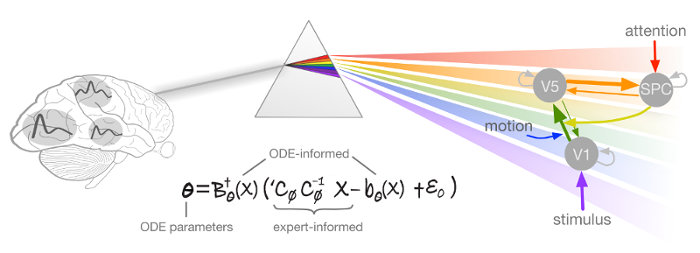
\includegraphics [width=4in]{cover_pic.png}

\end{par} \vspace{1em}
\begin{par}
Authors: \textbf{Nico Stephan Gorbach} and \textbf{Stefan Bauer}, email: \begin{verbatim}nico.gorbach@gmail.com\end{verbatim}
\end{par} \vspace{1em}
\begin{par}
Instructional code for the NIPS (2018) paper " \textbf{Scalable Variational Inference for Dynamical Systems} " by Nico S. Gorbach, Stefan Bauer and Joachim M. Buhmann. The paper is available at \begin{verbatim}https://papers.nips.cc/paper/7066-scalable-variational-inference-for-dynamical-systems.pdf\end{verbatim}. Please cite our paper if you use our program for a further publication. Part of the derivation below is described in Wenk et al. (2018).
\end{par} \vspace{1em}
\begin{par}
Example dynamical system used in this code: Lotka-Volterra system with \textbf{half} of the time points \textbf{unobserved}. The ODE parameters are also unobserved.
\end{par} \vspace{1em}

\subsection*{Contents}

\begin{itemize}
\setlength{\itemsep}{-1ex}
   \item Advantages of Variational Gradient Matching
   \item Simulation Settings
   \item User Input
   \item Import ODEs
   \item Mass Action Dynamical Systems
   \item Simulate Trajectory Observations
   \item Prior on States and State Derivatives
   \item Matching Gradients
   \item State Couplings in ODEs
   \item Rewrite ODEs as Linear Combination in Parameters
   \item Posterior over ODE Parameters
   \item Rewrite ODEs as Linear Combination in Individual States
   \item Posterior over Individual States
   \item Mean-field Variational Inference
   \item Fitting observations of state trajectories
   \item Coordinate Ascent Variational Gradient Matching
   \item Time Taken
   \item References
   \item Subroutines
\end{itemize}


\subsection*{Advantages of Variational Gradient Matching}

\begin{par}
The essential idea of gradient matching (Calderhead et al., 2002) is to match the gradient governed by the ODEs with that inferred from the observations. In contrast to previous approaches gradient matching introduces a prior over states instead of a prior over ODE parameters. The advantages of gradients matching is two-fold:
\end{par} \vspace{1em}
\begin{enumerate}
\setlength{\itemsep}{-1ex}
   \item A prior over the functional form of state dynamics as opposed to ODE parameters facilitates a more expert-aware estimation of ODE parameters since experts can provide a better \textit{a priori} description of state dynamics than ODE parameters.
   \item Gradient matching yields a global gradient as opposed to a local one which offers significant computational advantages and provides access to a rich source of sophisticated optimization tools.
\end{enumerate}
\begin{par}
Clear workspace and close figures
\end{par} \vspace{1em}
\begin{verbatim}
clear all; close all;
\end{verbatim}


\subsection*{Simulation Settings}

\begin{verbatim}
simulation.state_obs_variance = @(mean)(bsxfun(@times,[2,2],...
    ones(size(mean))));              % observation noise
simulation.ode_param = [10,28,8/3];  % true ODE parameters;
simulation.final_time = 20;          % end time for integration
simulation.int_interval = 0.01;      % integration interval
simulation.time_samp = 0:0.1:simulation.final_time; % sample times for observations
simulation.init_val = -7.*ones(1,3); % initial state values

%symbols of observed states that appear in the 'ODEs.txt' file.
simulation.observed_states = {'[x]','[z]'};
\end{verbatim}


\subsection*{User Input}

\begin{par}
\ensuremath{\backslash}subsection\{ Path to ODEs \}
\end{par} \vspace{1em}
\begin{verbatim}
odes_path = 'Lorenz_attractor_ODEs.txt';
\end{verbatim}
\begin{par}
\ensuremath{\backslash}subsection\{ Symbols \} symbols of states and parameters in the '\_ODEs.txt' file
\end{par} \vspace{1em}
\begin{par}
States $\mathbf{x}$:
\end{par} \vspace{1em}
\begin{verbatim}
symbols.state = {'[x]','[y]','[z]'}; % symbols of states in 'ODEs.txt' file
\end{verbatim}
\begin{par}
ODE parameters $\theta$ (symbols of parameters in 'ODEs.txt' file):
\end{par} \vspace{1em}
\begin{verbatim}
symbols.param = {'[\sigma]','[\rho]','[\beta]'};
\end{verbatim}
\begin{par}
\ensuremath{\backslash}subsection\{ Kernel \}
\end{par} \vspace{1em}
\begin{par}
Kernel parameters $\phi$:
\end{par} \vspace{1em}
\begin{verbatim}
kernel.param = [10,0.2];             % set values of rbf kernel parameters
\end{verbatim}
\begin{par}
Error variance on state derivatives (i.e. $\gamma$):
\end{par} \vspace{1em}
\begin{verbatim}
state.derivative_variance = 6*ones(1,length(symbols.state)); % gamma for gradient matching model
\end{verbatim}
\begin{par}
\ensuremath{\backslash}subsection\{ Estimation times \}
\end{par} \vspace{1em}
\begin{verbatim}
time.est = 0:0.1:20;                 % estimation times
\end{verbatim}
\begin{par}
\ensuremath{\backslash}subsection\{ Type of pseudo-inverse \} Type of pseudo inverse; options: 'Moore-Penrose' or 'modified Moore-Penrose'
\end{par} \vspace{1em}
\begin{verbatim}
opt_settings.pseudo_inv_type = 'Moore-Penrose';
\end{verbatim}
\begin{par}
\ensuremath{\backslash}subsection\{ Optimization settings \}
\end{par} \vspace{1em}
\begin{verbatim}
opt_settings.coord_ascent_numb_iter = 40;  % number of coordinate ascent iterations

% The observed state trajectories are clamped to the trajectories
% determined by standard GP regression (Boolean)
opt_settings.clamp_obs_state_to_GP_fit = true;
\end{verbatim}
\begin{par}
Plot settings: layout and size
\end{par} \vspace{1em}
\begin{verbatim}
plot_settings.size = [1600, 800]; plot_settings.layout = [2,2];
\end{verbatim}


\subsection*{Import ODEs}

\begin{verbatim}
ode = import_odes(symbols,odes_path);
\end{verbatim}
\begin{verbatim}
disp('ODEs:'); disp(ode.raw)
\end{verbatim}

        \color{lightgray} \begin{verbatim}ODEs:
    '[\sigma] .* ([y] - [x])'
    '[\rho] .* [x] - [y] - [x] .* [z]'
    '[x] .* [y] - [\beta] .* [z]'

\end{verbatim} \color{black}
    

\subsection*{Mass Action Dynamical Systems}

\begin{par}
A deterministic dynamical system is represented by a set of $K$ ordinary differential equations (ODEs) with model parameters $\theta \in R^d$ that describe the evolution of $K$ states $\mathbf{x}(t) = [x_1(t),\ldots, x_K(t)]^T$ such that:
\end{par} \vspace{1em}
\begin{par}
$\dot{\mathbf{x}}(t) = \frac{d \mathbf{x}(t)}{d t} = \mathbf{f}(\mathbf{x}(t),\theta) \qquad (1)$.
\end{par} \vspace{1em}
\begin{par}
A sequence of observations, $\mathbf{y}(t)$, is usually contaminated by measurement error which we assume to be normally distributed with zero mean and variance for each of the $K$ states, i.e. $\mathbf{E}\sim \mathcal{N}(\mathbf{E};\mathbf{0},\mathbf{D})$, with $\mathbf{D}_{ik}=\sigma_k ^2 \delta_{ik}$. For $N$ distinct time points the overall system may therefore be summarized as:
\end{par} \vspace{1em}
\begin{par}
$\mathbf{Y} = \mathbf{X} + \mathbf{E}$,
\end{par} \vspace{1em}
\begin{par}
where
\end{par} \vspace{1em}
\begin{par}
$\mathbf{X} = [\mathbf{x}(t_1),\ldots,\mathbf{x}(t_N)] = [\mathbf{x}_1,\ldots,\mathbf{x}_K]^T$,
\end{par} \vspace{1em}
\begin{par}
$\mathbf{Y} = [\mathbf{y}(t_1),\ldots,\mathbf{y}(t_N)] = [\mathbf{y}_1,\ldots,\mathbf{y}_K]^T$,
\end{par} \vspace{1em}
\begin{par}
and $\mathbf{x}_k = [x_k(t_1),\ldots,x_k(t_N)]^T$ is the $k$'th state sequence and $\mathbf{y}_k = [y_k(t_1),$ $\ldots,y_k(t_N)]^T$ are the observations. Given the observations $\mathbf{Y}$ and the description of the dynamical system (1), the aim is to estimate both state variables $\mathbf{X}$ and parameters $\theta$.
\end{par} \vspace{1em}
\begin{par}
We consider only dynamical systems that are locally linear with respect to ODE parameters $\theta$ and individual states $\mathbf{x}_u$. Such ODEs include mass-action kinetics and are given by:
\end{par} \vspace{1em}
\begin{par}
$f_{k}(\mathbf{x}(t),\theta) = \sum_{i=1} \theta_{ki} \prod_{j \in \mathcal{M}_{ki}} x_j \qquad (2)$,
\end{par} \vspace{1em}
\begin{par}
with $\mathcal{M}_{ki} \subseteq \{ 1, \dots, K\}$ describing the state variables in each factor of the equation (i.e. the functions are linear in parameters and contain arbitrary large products of monomials of the states).
\end{par} \vspace{1em}


\subsection*{Simulate Trajectory Observations}

\begin{par}
\ensuremath{\backslash}subsection\{ Generate ground truth by numerical integration \}
\end{par} \vspace{1em}
\begin{verbatim}
[state,time,ode] = generate_ground_truth(time,state,ode,symbols,simulation,...
    odes_path);
\end{verbatim}
\begin{par}
\ensuremath{\backslash}subsection\{ Generate state observations \}
\end{par} \vspace{1em}
\begin{verbatim}
if ~iscell(simulation.observed_states)
    ratio_observed = simulation.observed_states;
    state_obs_idx = zeros(1,simulation.numb_odes,'logical');
    idx = randperm(simulation.numb_odes);
    idx = idx(1:floor(simulation.numb_odes * ratio_observed));
    state_obs_idx(idx) = 1;
    simulation.observed_states = symbols.state(state_obs_idx);
end

[state,time,obs_to_state_relation] = generate_state_obs(state,time,simulation,...
    symbols);
\end{verbatim}
\begin{par}
\ensuremath{\backslash}subsection\{ Symbols \}
\end{par} \vspace{1em}
\begin{verbatim}
state.sym.mean = sym('x%d%d',[length(time.est),length(ode.system)]);
state.sym.variance = sym('sigma%d%d',[length(time.est),length(ode.system)]);
ode_param.sym.mean = sym('param%d',[length(symbols.param),1]);
assume(ode_param.sym.mean,'real');
\end{verbatim}
\begin{par}
\ensuremath{\backslash}subsection\{ Setup plots \}
\end{par} \vspace{1em}
\begin{par}
Only the state dynamics are (partially) observed.
\end{par} \vspace{1em}
\begin{verbatim}
[h_states,h_param,p] = setup_plots(state,time,simulation,symbols,plot_settings);

tic; %start timer
\end{verbatim}


\subsection*{Prior on States and State Derivatives}

\begin{par}
Gradient matching with Gaussian processes assumes a joint Gaussian process prior on states and their derivatives:
\end{par} \vspace{1em}
\begin{par}
$\left(\begin{array}{c} \mathbf{X} \\ \dot{\mathbf{X}} \end{array}\right)  \sim \mathcal{N} \left( \begin{array}{c} \mathbf{X} \\ \dot{\mathbf{X}} \end{array}; \begin{array}{c}  \mathbf{0} \\ \mathbf{0}  \end{array}, \begin{array}{cc}  \mathbf{C}_{\phi} & \mathbf{C}_{\phi}' \\ '\mathbf{C}_{\phi} &  \mathbf{C}_{\phi}'' \end{array} \right) \qquad (3)$,
\end{par} \vspace{1em}
\begin{par}
$\mathrm{cov}(x_k(t), x_k(t)) = C_{\phi_k}(t,t')$
\end{par} \vspace{1em}
\begin{par}
$\mathrm{cov}(\dot{x}_k(t), x_k(t)) = \frac{\partial C_{\phi_k}(t,t') }{\partial t} =: C_{\phi_k}'(t,t')$
\end{par} \vspace{1em}
\begin{par}
$\mathrm{cov}(x_k(t), \dot{x}_k(t)) = \frac{\partial C_{\phi_k}(t,t') }{\partial t'} =: {'C_{\phi_k}(t,t')}$
\end{par} \vspace{1em}
\begin{par}
$\mathrm{cov}(\dot{x}_k(t), \dot{x}_k(t)) = \frac{\partial C_{\phi_k}(t,t') }{\partial t \partial t'} =: C_{\phi_k}''(t,t')$.
\end{par} \vspace{1em}


\subsection*{Matching Gradients}

\begin{par}
Given the joint distribution over states and their derivatives (3) as well as the ODEs (2), we therefore have two expressions for the state derivatives:
\end{par} \vspace{1em}
\begin{par}
$\dot{\mathbf{X}} = \mathbf{F} + \epsilon_1, \epsilon_1 \sim \mathcal{N}\left(\epsilon_1;\mathbf{0}, \mathbf{I}\gamma \right)$
\end{par} \vspace{1em}
\begin{par}
$\dot{\mathbf{X}} = {'\mathbf{C}_{\phi}} \mathbf{C}_{\phi}^{-1} ~\mathbf{X} + \epsilon_2, \epsilon_2 \sim \mathcal{N}\left(\epsilon_2;\mathbf{0}, \mathbf{A} \right)$
\end{par} \vspace{1em}
\begin{par}
where $\mathbf{F} := \mathbf{f}(\mathbf{X},\theta)$, $\mathbf{A} := \mathbf{C}_{\phi}'' -  {'\mathbf{C}_{\phi}} \mathbf{C}_{\phi}^{-1} \mathbf{C}_{\phi}'$ and $\gamma$ is the error variance in the ODEs. Note that, in a deterministic system, the output of the ODEs $\mathbf{F}$ should equal the state derivatives $\dot{\mathbf{X}}$. However, in the first equation above we relax this contraint by adding stochasticity to the state derivatives $\dot{\mathbf{X}}$ in order to compensate for a potential model mismatch. The second equation above is obtained by deriving the conditional distribution for $\dot{\mathbf{X}}$ from the joint distribution in equation (3). Equating the two expressions in the equations above we can eliminate the unknown state derivatives $\dot{\mathbf{X}}$:
\end{par} \vspace{1em}
\begin{par}
$\mathbf{F} = {'\mathbf{C}_{\phi}} \mathbf{C}_{\phi}^{-1} ~\mathbf{X} + \epsilon_0 \qquad (4)$,
\end{par} \vspace{1em}
\begin{par}
with $\epsilon_0 := \epsilon_2 - \epsilon_1$.
\end{par} \vspace{1em}
\begin{verbatim}
[dC_times_invC,inv_C,A_plus_gamma_inv] = kernel_function(kernel,state,time.est);
\end{verbatim}


\subsection*{State Couplings in ODEs}

\begin{verbatim}
coupling_idx = find_state_couplings_in_odes(ode,symbols);
\end{verbatim}


\subsection*{Rewrite ODEs as Linear Combination in Parameters}

\begin{par}
We rewrite the ODEs in equation (2) as a linear combination in the parameters:
\end{par} \vspace{1em}
\begin{par}
$\mathbf{B}_{\theta k} \theta + \mathbf{b}_{\theta k} \stackrel{!}{=} \mathbf{f}_k(\mathbf{X},\theta) \qquad (5)$,
\end{par} \vspace{1em}
\begin{par}
where matrices $\mathbf{B}_{\theta k}$ and $\mathbf{b}_{\theta k}$ are defined such that the ODEs $\mathbf{f}_k(\mathbf{X},\theta)$ are expressed as a linear combination in $\theta$.
\end{par} \vspace{1em}
\begin{verbatim}
[ode_param.lin_comb.B,ode_param.lin_comb.b] = ...
    rewrite_odes_as_linear_combination_in_parameters(ode,symbols);
\end{verbatim}


\subsection*{Posterior over ODE Parameters}

\begin{par}
Inserting (5) into (4) and solving for $\theta$ yields:
\end{par} \vspace{1em}
\begin{par}
$\theta = \mathbf{B}_{\theta}^+ \left( {'\mathbf{C}_{\phi}} \mathbf{C}_{\phi}^{-1} \mathbf{X} - \mathbf{b}_{\theta} + \epsilon_0 \right)$,
\end{par} \vspace{1em}
\begin{par}
where $\mathbf{B}_{\theta}^+$ denotes the pseudo-inverse of $\mathbf{B}_{\theta}$.
\end{par} \vspace{1em}
\begin{par}
Since $\mathbf{C}_{\phi}$ is block diagonal we can rewrite the expression above as:
\end{par} \vspace{1em}
\begin{par}
$\theta = \left( \mathbf{B}_{\theta}^T \mathbf{B}_{\theta} \right)^{-1} \mathbf{B}_{\theta}^T  \left( \sum_k {'\mathbf{C}_{\phi_k}} \mathbf{C}_{\boldmath\phi_k}^{-1} \mathbf{X}_k - \mathbf{b}_{\theta k} + \boldmath\epsilon_0^{(k)} \right)$,
\end{par} \vspace{1em}
\begin{par}
$= \left( \mathbf{B}_{\theta}^T \mathbf{B}_{\theta} \right)^{-1} \left( \sum_k \mathbf{B}_{\theta k}^T \left( {'\mathbf{C}_{\phi_k}} \mathbf{C}_{\boldmath\phi_k}^{-1} \mathbf{X}_k - \mathbf{b}_{\theta k} + \boldmath\epsilon_0^{(k)} \right) \right)$,
\end{par} \vspace{1em}
\begin{par}
where we subsitute the Moore-Penrose inverse for the pseudo-inverse (i.e. $\mathbf{B}_{\theta}^+ = \left( \mathbf{B}_{\theta}^T \mathbf{B}_{\theta} \right)^{-1} \mathbf{B}_{\theta}^T$).
\end{par} \vspace{1em}
\begin{par}
We can therefore derive the posterior distribution over ODE parameters:
\end{par} \vspace{1em}
\begin{par}
$p(\theta \mid \mathbf{X}, \phi, \gamma) = \mathcal{N}\left(\theta ; \mathbf{B}_{\theta}^+ ~ \left( {'\mathbf{C}_{\phi}} \mathbf{C}_{\phi}^{-1} \mathbf{X} - \mathbf{b}_{\theta} \right), ~ \mathbf{B}_{\theta}^+ ~ (\mathbf{A} + \mathbf{I}\gamma) ~ \mathbf{B}_{\theta}^{+T} \right)$
\end{par} \vspace{1em}
\begin{par}
$= \mathcal{N}\left(\theta ; \left( \mathbf{B}_{\theta}^T \mathbf{B}_{\theta} \right)^{-1} \left( \sum_k \mathbf{B}_{\theta k}^T ~ \left( {'\mathbf{C}_{\phi k}} \mathbf{C}_{\phi k}^{-1} \mathbf{X}_k - \mathbf{b}_{\theta k} \right) \right), ~ \mathbf{B}_{\theta}^+ ~ (\mathbf{A} + \mathbf{I}\gamma) ~ \mathbf{B}_{\theta}^{+T} \right)$
\end{par} \vspace{1em}
\begin{par}
$= \prod_k \mathcal{N}\left(\theta ; \left( \mathbf{B}_{\theta}^T \mathbf{B}_{\theta} \right)^{-1} \left( \mathbf{B}_{\theta k}^T ~ \left( {'\mathbf{C}_{\phi k}} \mathbf{C}_{\phi k}^{-1} \mathbf{X}_k - \mathbf{b}_{\theta k} \right) \right), ~ \mathbf{B}_{\theta k}^+ ~ (\mathbf{A}_k + \mathbf{I}\gamma) ~ \mathbf{B}_{\theta k}^{+T} \right) \qquad (6)$
\end{par} \vspace{1em}


\subsection*{Rewrite ODEs as Linear Combination in Individual States}

\begin{par}
We rewrite the expression $\mathbf{f}(\mathbf{X},\theta) - {'\mathbf{C}}_{\phi} \mathbf{C}_{\phi}^{-1} \mathbf{X}$ in equation (4) as a linear combination in the individual state $\mathbf{x}_u$:
\end{par} \vspace{1em}
\begin{par}
$\mathbf{R}_{uk} \mathbf{x}_u + \mathbf{r}_{uk} \stackrel{!}{=} \mathbf{f}_k(\mathbf{X},\theta)$.
\end{par} \vspace{1em}
\begin{par}
where matrices $\mathbf{R}_{uk}$ and $\mathbf{r}_{uk}$ are defined such that the ODE $\mathbf{f}_k(\mathbf{X},\theta)$ is expressed as a linear combination in the individual state $\mathbf{x}_u$.
\end{par} \vspace{1em}
\begin{verbatim}
[state.lin_comb.R,state.lin_comb.r] = ...
    rewrite_odes_as_linear_combination_in_ind_states(ode,symbols,coupling_idx.states);
\end{verbatim}


\subsection*{Posterior over Individual States}

\begin{par}
Given the linear combination of the ODEs w.r.t. an individual state, we define the matrices $\mathbf{B}_u$ and $\mathbf{b}_u$ such that the expression $\mathbf{f}(\mathbf{X},\theta) - {'\mathbf{C}}_{\phi} \mathbf{C}_{\phi}^{-1} \mathbf{X}$ is rewritten as a linear combination in an individual state:
\end{par} \vspace{1em}
\begin{par}
$\mathbf{B}_{u} \mathbf{x}_u + \mathbf{b}_{u} \stackrel{!}{=} \mathbf{f}(\mathbf{X},\theta) \qquad (7)$.
\end{par} \vspace{1em}
\begin{par}
Inserting (7) into (4) and solving for $\mathbf{x}_u$ yields:
\end{par} \vspace{1em}
\begin{par}
$\mathbf{x}_u = \mathbf{B}_{u}^+ \left( \epsilon_0 -\mathbf{b}_{u} \right)$,
\end{par} \vspace{1em}
\begin{par}
Since $\mathbf{C}_{\phi}$ is block diagonal we can rewrite the expression above as:
\end{par} \vspace{1em}
\begin{par}
$\mathbf{x}_u = \left( \mathbf{B}_{u} \mathbf{B}_{u}^T \right)^{-1} \mathbf{B}_{u}^T \sum_k \left(\epsilon_0^{(k)} -\mathbf{b}_{uk} \right)$
\end{par} \vspace{1em}
\begin{par}
$= \left( \mathbf{B}_{u} \mathbf{B}_{u}^T \right)^{-1} \sum_k \mathbf{B}_{uk}^T \left(\epsilon_0^{(k)} -\mathbf{b}_{uk} \right)$,
\end{par} \vspace{1em}
\begin{par}
where $\mathbf{B}_{u}^+$ denotes the pseudo-inverse of $\mathbf{B}_{u}$. We can therefore derive the posterior distribution over an individual state $\mathbf{x}_u$:
\end{par} \vspace{1em}
\begin{par}
$p(\mathbf{x}_u \mid \mathbf{X}_{-u}, \phi, \gamma) = \mathcal{N}\left(\mathbf{x}_u ; -\mathbf{B}_{u}^+ \mathbf{b}_u, ~\mathbf{B}_u^{+} ~ (\mathbf{A} + \mathbf{I}\gamma) ~ \mathbf{B}_u^{+T} \right)$
\end{par} \vspace{1em}
\begin{par}
$= \mathcal{N}\left(\mathbf{x}_u ; \left( \mathbf{B}_{u} \mathbf{B}_{u}^T \right)^{-1} \left( - \sum_k \mathbf{B}_{uk}^T \mathbf{b}_{uk} \right), ~\mathbf{B}_{u}^{+} ~ (\mathbf{A} + \mathbf{I}\gamma) ~ \mathbf{B}_u^{+T} \right) \qquad (8)$,
\end{par} \vspace{1em}
\begin{par}
with $\mathbf{X}_{-u}$ denoting the set of all states except state $\mathbf{x}_u$.
\end{par} \vspace{1em}


\subsection*{Mean-field Variational Inference}

\begin{par}
To infer the parameters $\theta$, we want to find the maximum a posteriori estimate (MAP):
\end{par} \vspace{1em}
\begin{par}
$\theta^* := arg \max_{\theta} ~ \ln p(\theta \mid \mathbf{Y},\phi,\gamma, \sigma)$
\end{par} \vspace{1em}
\begin{par}
$= arg\max_{\theta} ~ \ln \int  p(\theta,\mathbf{X} \mid \mathbf{Y},\phi,\gamma,\boldmath\sigma) d\mathbf{X}$
\end{par} \vspace{1em}
\begin{par}
$= arg\max_{\theta} ~ \ln \int p(\theta \mid \mathbf{X},\phi,\gamma) p(\mathbf{X} \mid \mathbf{Y}, \phi,\boldmath\sigma) d\mathbf{X} \qquad (9)$.
\end{par} \vspace{1em}
\begin{par}
However, the integral above is intractable due to the strong couplings induced by the nonlinear ODEs $\mathbf{f}$ which appear in the term $p(\theta \mid \mathbf{X},\phi,\gamma)$.
\end{par} \vspace{1em}
\begin{par}
We use mean-field variational inference to establish variational lower bounds that are analytically tractable by decoupling state variables from the ODE parameters as well as decoupling the state variables from each other. Note that, since the ODEs described by equation (2) are \textbf{locally linear}, both conditional distributions $p(\theta \mid \mathbf{X},\mathbf{Y},\phi,\gamma,\boldmath\sigma)$ (equation (6)) and $p(\mathbf{x}_u \mid \theta, \mathbf{X}_{-u},\mathbf{Y},\phi,\gamma,\boldmath\sigma)$ (equation (8)) are analytically tractable and Gaussian distributed as mentioned previously.
\end{par} \vspace{1em}
\begin{par}
The decoupling is induced by designing a variational distribution $Q(\theta,\mathbf{X})$ which is restricted to the family of factorial distributions:
\end{par} \vspace{1em}
\begin{par}
$\mathcal{Q} := \bigg{\{} Q : Q(\theta,\mathbf{X}) = q(\theta) \prod_u q(\mathbf{x}_u) \bigg{\}}$.
\end{par} \vspace{1em}
\begin{par}
The particular form of $q(\theta)$ and $q(\mathbf{x}_u)$ are designed to be Gaussian distributed which places them in the same family as the true full conditional distributions. To find the optimal factorial distribution we minimize the Kullback-Leibler divergence between the variational and the true posterior distribution:
\end{par} \vspace{1em}
\begin{par}
$\hat{Q} := arg \min_{Q(\theta,\mathbf{X}) \in \mathcal{Q}} \mathrm{KL} \left[ Q(\theta,\mathbf{X}) \mid \mid p(\theta,\mathbf{X} \mid \mathbf{Y},\phi, \gamma,\boldmath\sigma) \right] \qquad (10)$,
\end{par} \vspace{1em}
\begin{par}
where $\hat{Q}$ is the proxy distribution. The proxy distribution that minimizes the KL-divergence (10) depends on the true full conditionals and is given by:
\end{par} \vspace{1em}
\begin{par}
$\hat{q}({\theta}) \propto \exp \left(~ E_{Q_{-\theta}} \ln p(\theta \mid \mathbf{X},\mathbf{Y},\phi,\gamma,\boldmath\sigma) ~\right) \qquad (11)$
\end{par} \vspace{1em}
\begin{par}
$\hat{q}(\mathbf{x}_u) \propto \exp\left( ~ E_{Q_{-u}} \ln p(\mathbf{x}_u \mid \theta, \mathbf{X}_{-u},\mathbf{Y},\phi,\gamma,\sigma) ~ \right) \qquad (12)$.
\end{par} \vspace{1em}


\subsection*{Fitting observations of state trajectories}

\begin{par}
We fit the observations of state trajectories by standard GP regression. The data-informed distribution $p(\mathbf{X} \mid \mathbf{Y}, \phi,\boldmath\sigma)$ in euqation (9) can be determined analytically using Gaussian process regression with the GP prior $p(\mathbf{X} \mid \phi) = \prod_k \mathcal{N}(\mathbf{x}_k ; \mathbf{0},\mathbf{C}_{\phi})$:
\end{par} \vspace{1em}
\begin{par}
$p(\mathbf{X} \mid \mathbf{Y}, \phi,\gamma) = \prod_k \mathcal{N}(\mathbf{x}_k ; \boldmath\mu_k(\mathbf{y}_k),\boldmath\Sigma_k)$,
\end{par} \vspace{1em}
\begin{par}
where $\boldmath\mu_k(\mathbf{y}_k) := \sigma_k^{-2} \left(\sigma_k^{-2} \mathbf{I} + \mathbf{C}_{\boldmath\phi_k}^{-1} \right)^{-1} \mathbf{y}_k$ and $\boldmath\Sigma_k ^{-1}:=\sigma_k^{-2} \mathbf{I} + \mathbf{C}_{\boldmath\phi_k}^{-1}$.
\end{par} \vspace{1em}
\begin{verbatim}
[mu,inv_sigma] = fitting_state_observations(state,inv_C,obs_to_state_relation,simulation);
\end{verbatim}


\subsection*{Coordinate Ascent Variational Gradient Matching}

\begin{par}
We minimize the KL-divergence in equation (10) by coordinate descent (where each step is analytically tractable) by iterating between determining the proxy for the distribution over ODE parameters $\hat{q}(\theta)$ and the proxies for the distribution over individual states $\hat{q}(\mathbf{x}_u)$.
\end{par} \vspace{1em}
\begin{verbatim}
state.proxy.mean = mu;  % Initialize the state estimation by the GP regression posterior
for i = 1:opt_settings.coord_ascent_numb_iter
\end{verbatim}
\begin{par}
\ensuremath{\backslash}subsection\{ Proxy for ODE parameters \}
\end{par} \vspace{1em}
\begin{par}
Expanding the proxy distribution in equation (11) for $\theta$ yields:
\end{par} \vspace{1em}
\begin{par}
$\hat{q}(\theta) \stackrel{(a)}{\propto} \exp \left( ~E_{Q_{-\theta}} \ln p(\theta \mid \mathbf{X},\mathbf{Y},\phi,\gamma,\sigma) ~ \right)$
\end{par} \vspace{1em}
\begin{par}
$\stackrel{(b)}{\propto} \exp \left( ~E_{Q_{-\theta}}  \ln \mathcal{N} \left( \theta; \mathbf{B}_{\theta}^+ ~ \left( '\mathbf{C}_{\phi} \mathbf{C}_{\phi}^{-1} \mathbf{X} - \mathbf{b}_{\theta} \right), ~ \mathbf{B}_{\theta}^+ ~ (\mathbf{A} + \mathbf{I}\gamma) ~ \mathbf{B}_{\theta}^{+T} \right) ~\right)$
\end{par} \vspace{1em}
\begin{par}
$= \exp \left( ~E_{Q_{-\theta}} \mathcal{N}\left(\theta ; \left( \mathbf{B}_{\theta}^T \mathbf{B}_{\theta} \right)^{-1} \left( \sum_k \mathbf{B}_{\theta k}^T ~ \left( {'\mathbf{C}_{\phi k}} \mathbf{C}_{\phi k}^{-1} \mathbf{X}_k - \mathbf{b}_{\theta k} \right) \right), ~ \mathbf{B}_{\theta}^+ ~ (\mathbf{A} + \mathbf{I}\gamma) ~ \mathbf{B}_{\theta}^{+T} \right) ~\right)$,
\end{par} \vspace{1em}
\begin{par}
which can be normalized analytically due to its exponential quadratic form. In (a) we recall that the ODE parameters depend only indirectly on the observations $\mathbf{Y}$ through the states $\mathbf{X}$ and in (b) we substitute $p(\theta \mid \mathbf{X},\phi,\gamma)$ by its density given in equation (6).
\end{par} \vspace{1em}
\begin{verbatim}
    [param_proxy_mean,param_proxy_inv_cov] = proxy_for_ode_parameters(state.proxy.mean,...
        dC_times_invC,ode_param.lin_comb,symbols,A_plus_gamma_inv,opt_settings);

    if i==1 || ~mod(i,1)
        plot_results(h_states,h_param,state,time,simulation,param_proxy_mean,...
            p,symbols,'not_final');
    end
\end{verbatim}

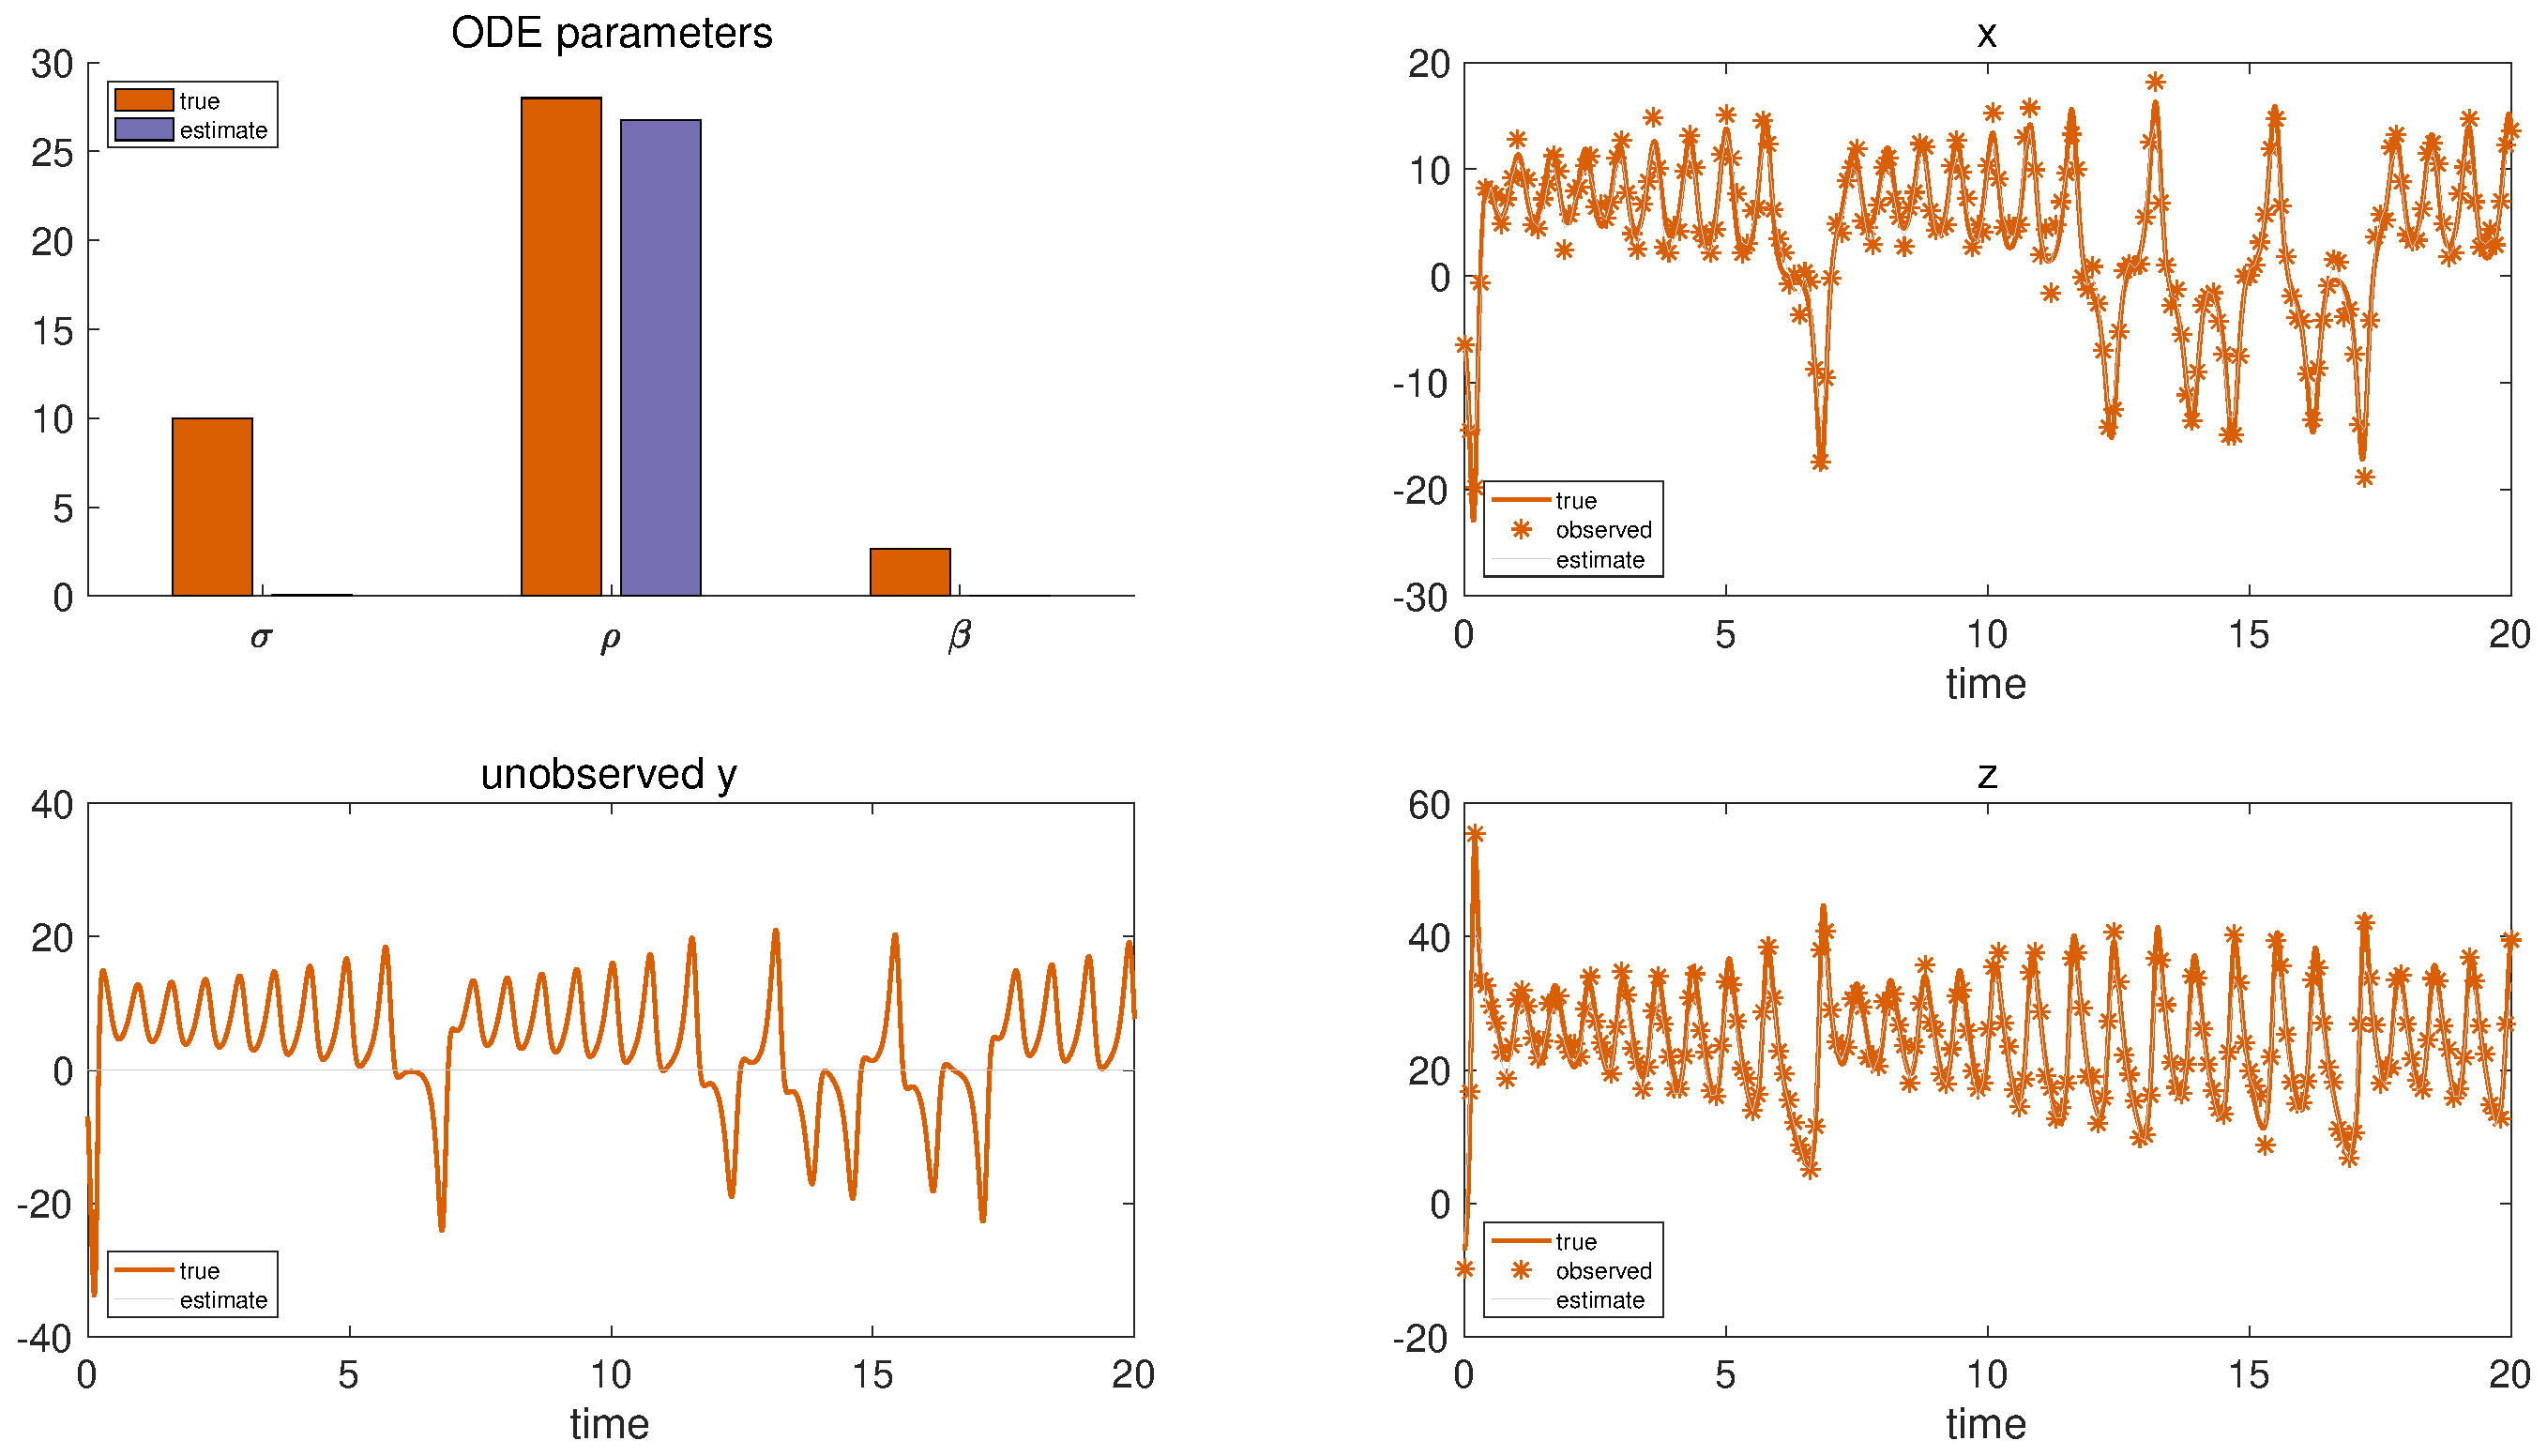
\includegraphics [width=4in]{Lorenz_attractor_4_05.eps}

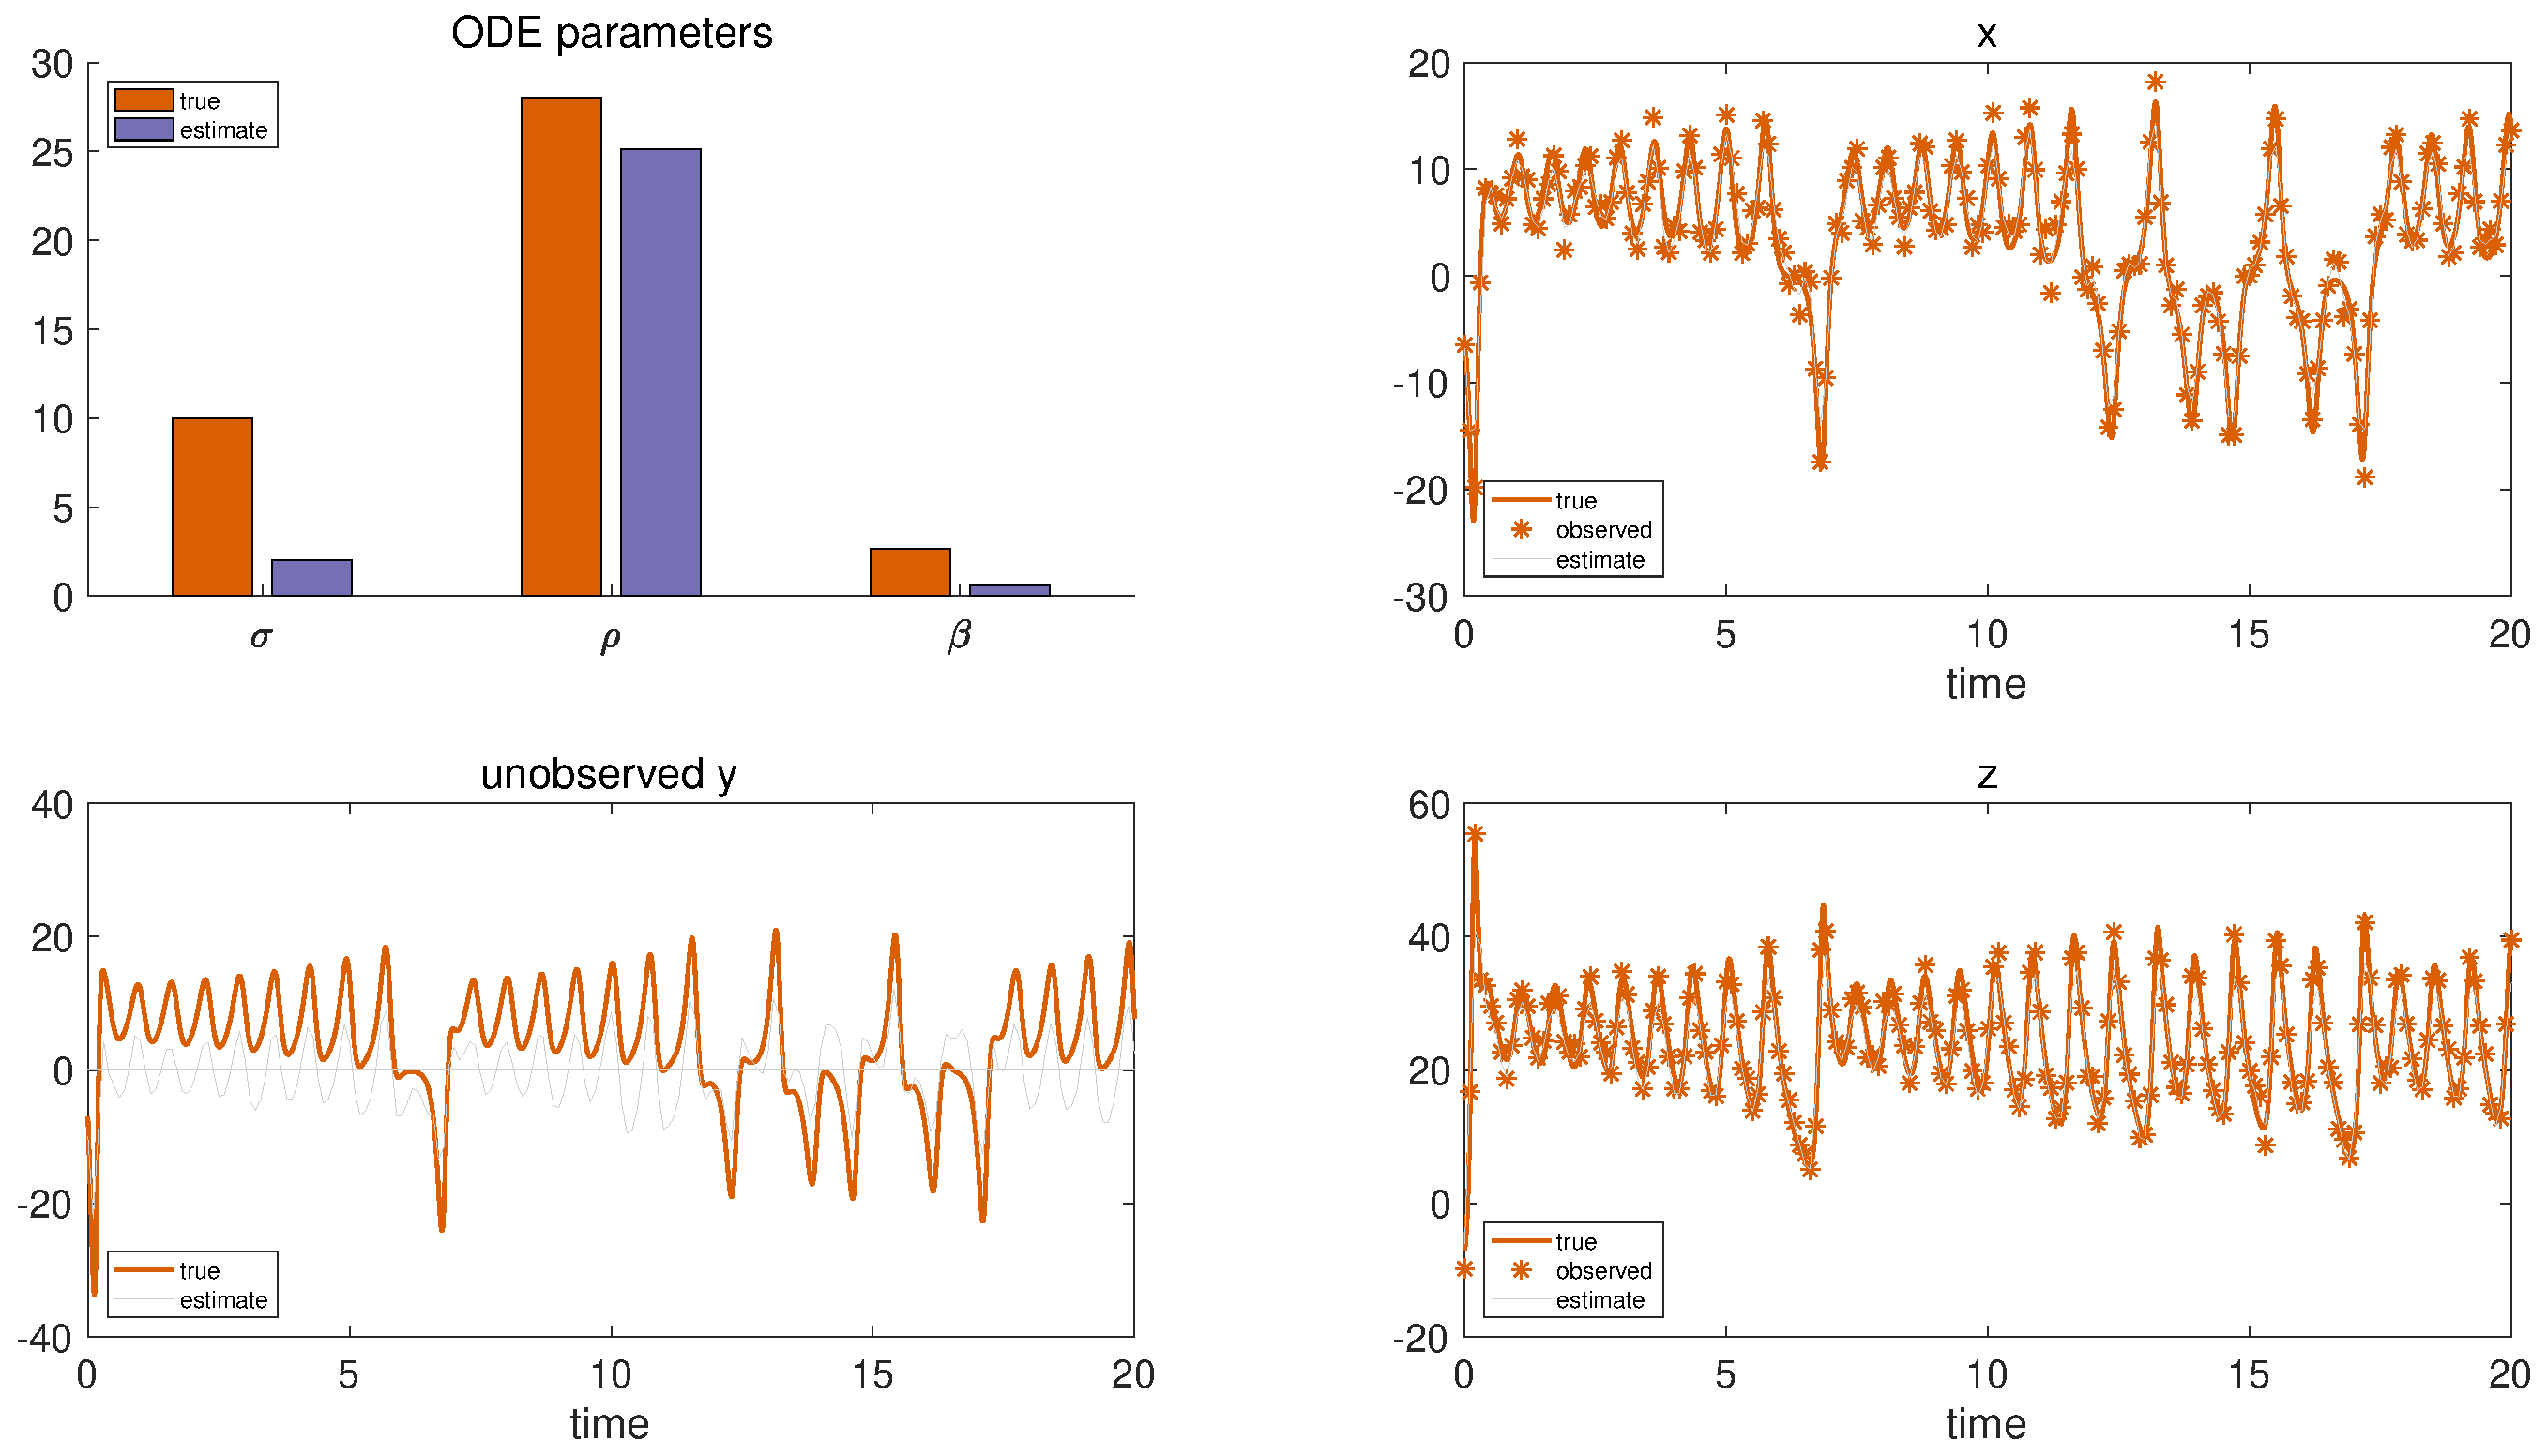
\includegraphics [width=4in]{Lorenz_attractor_4_06.eps}

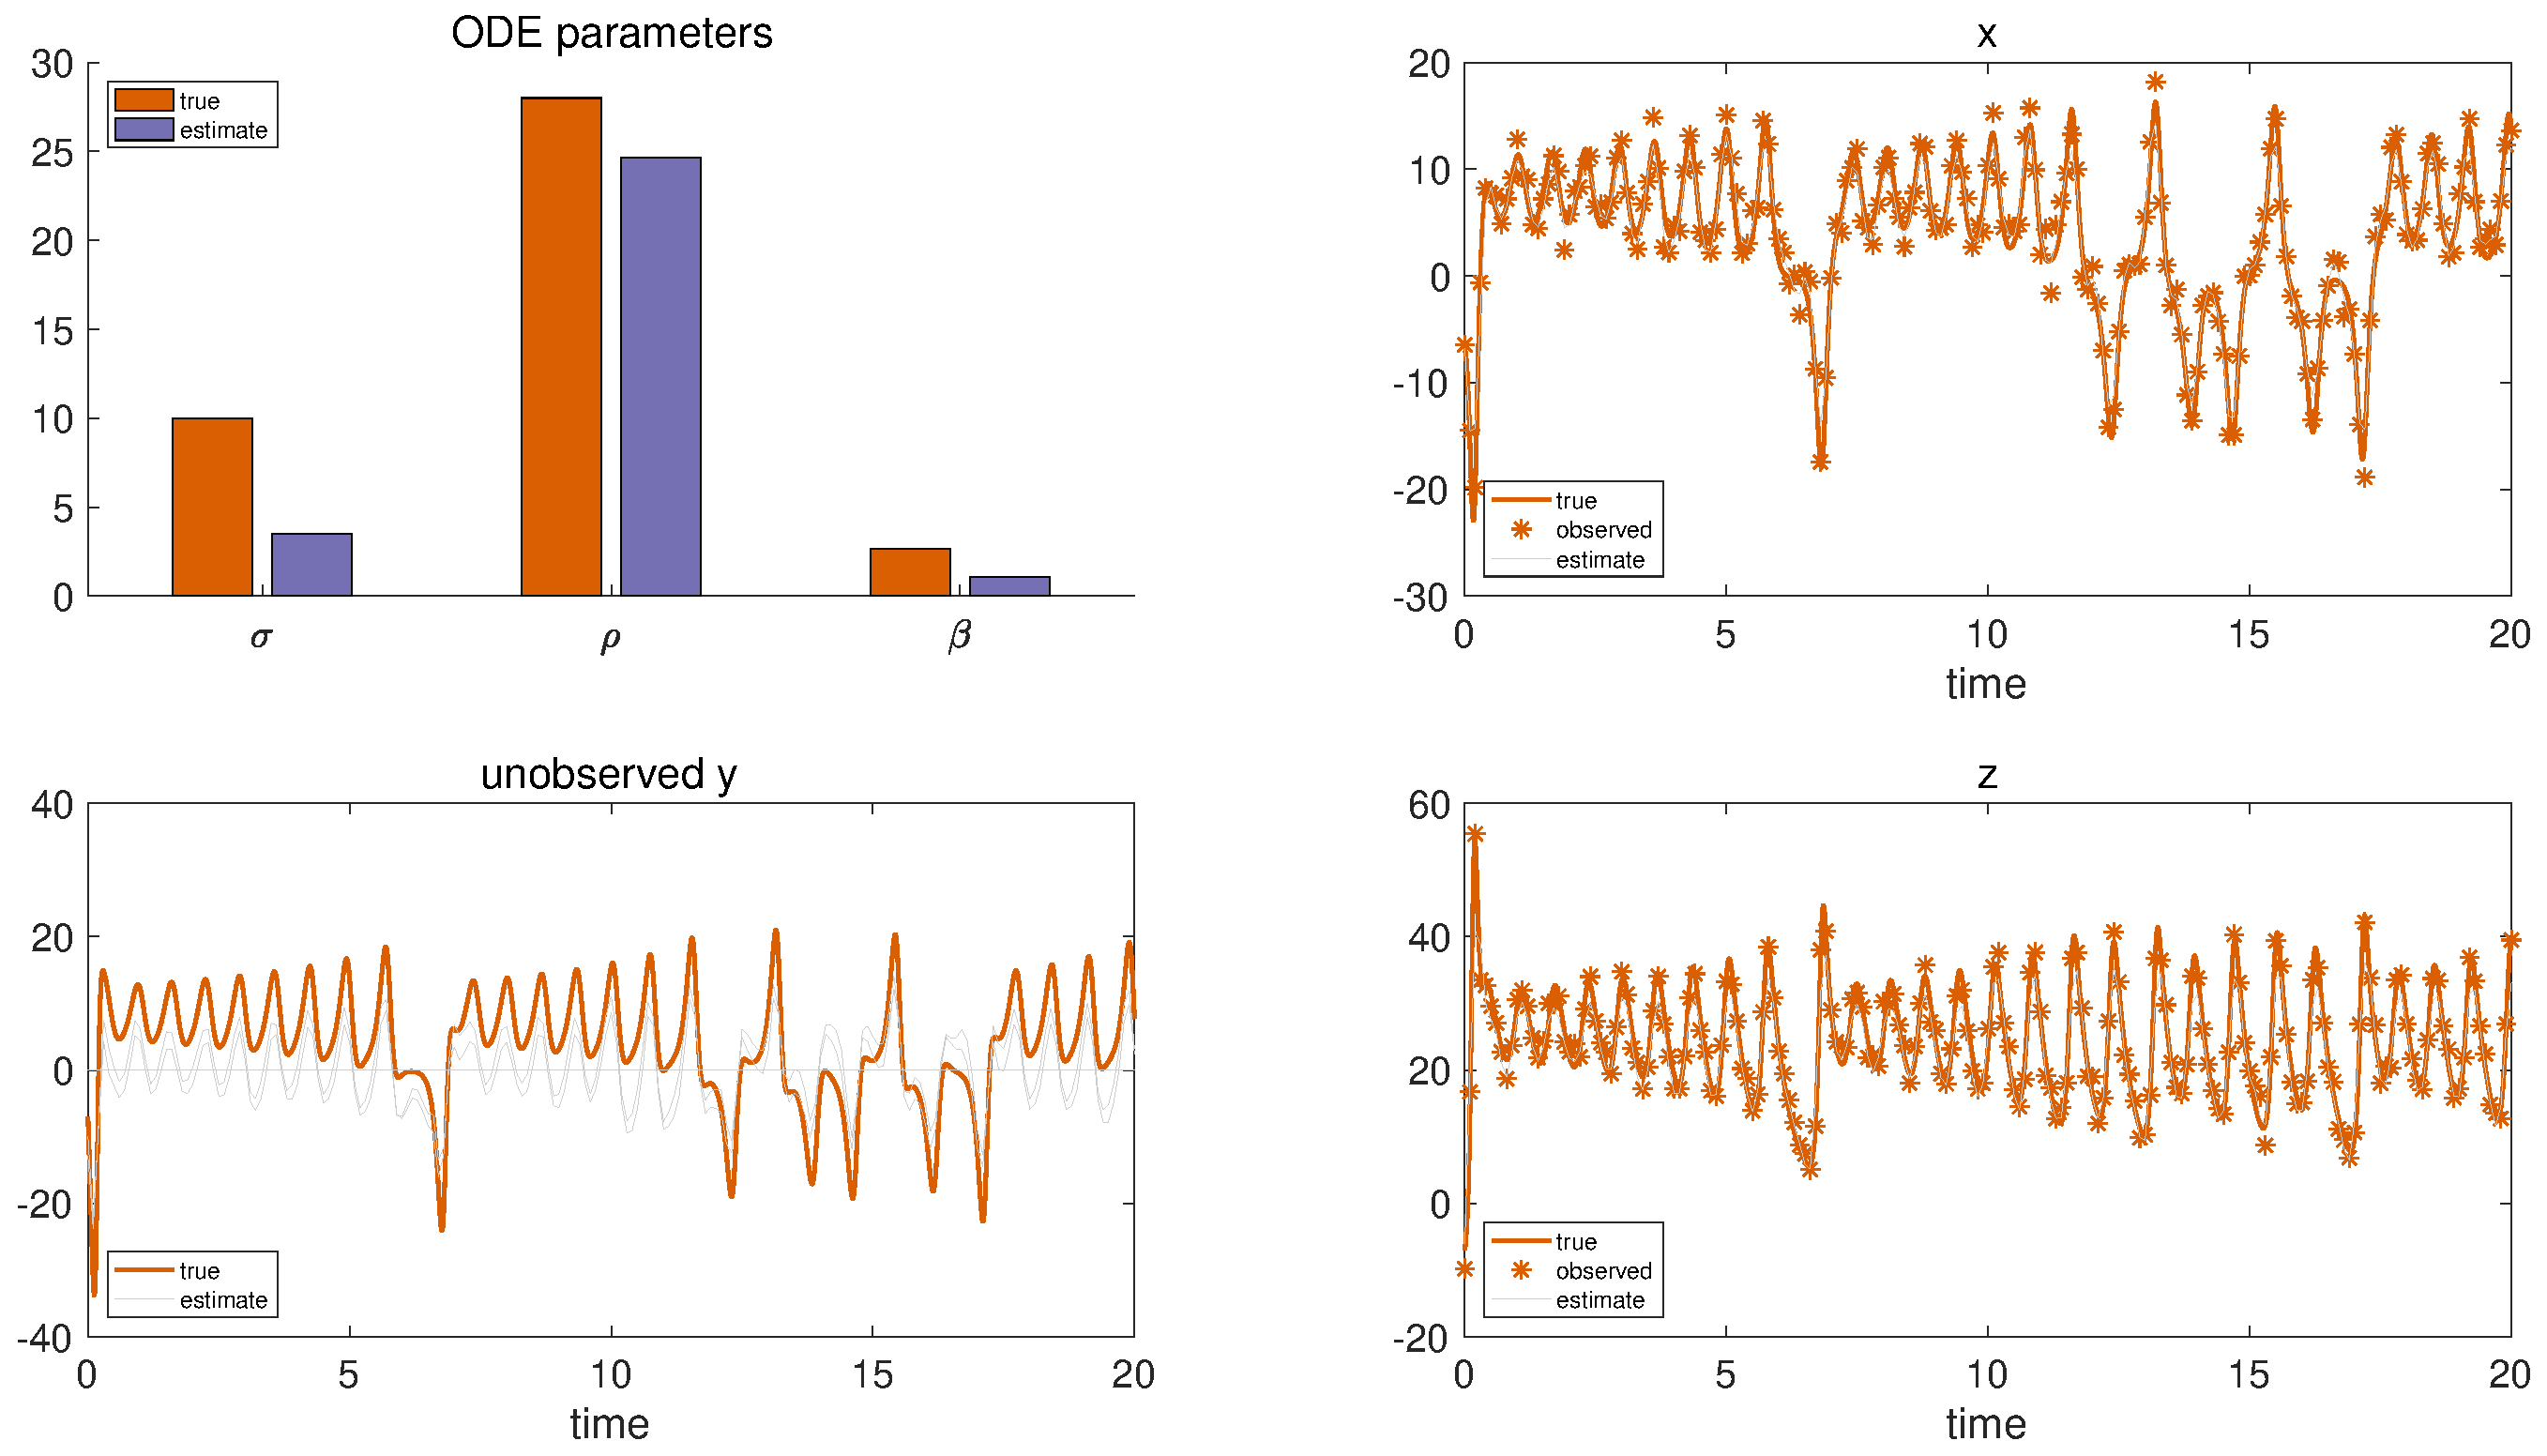
\includegraphics [width=4in]{Lorenz_attractor_4_07.eps}

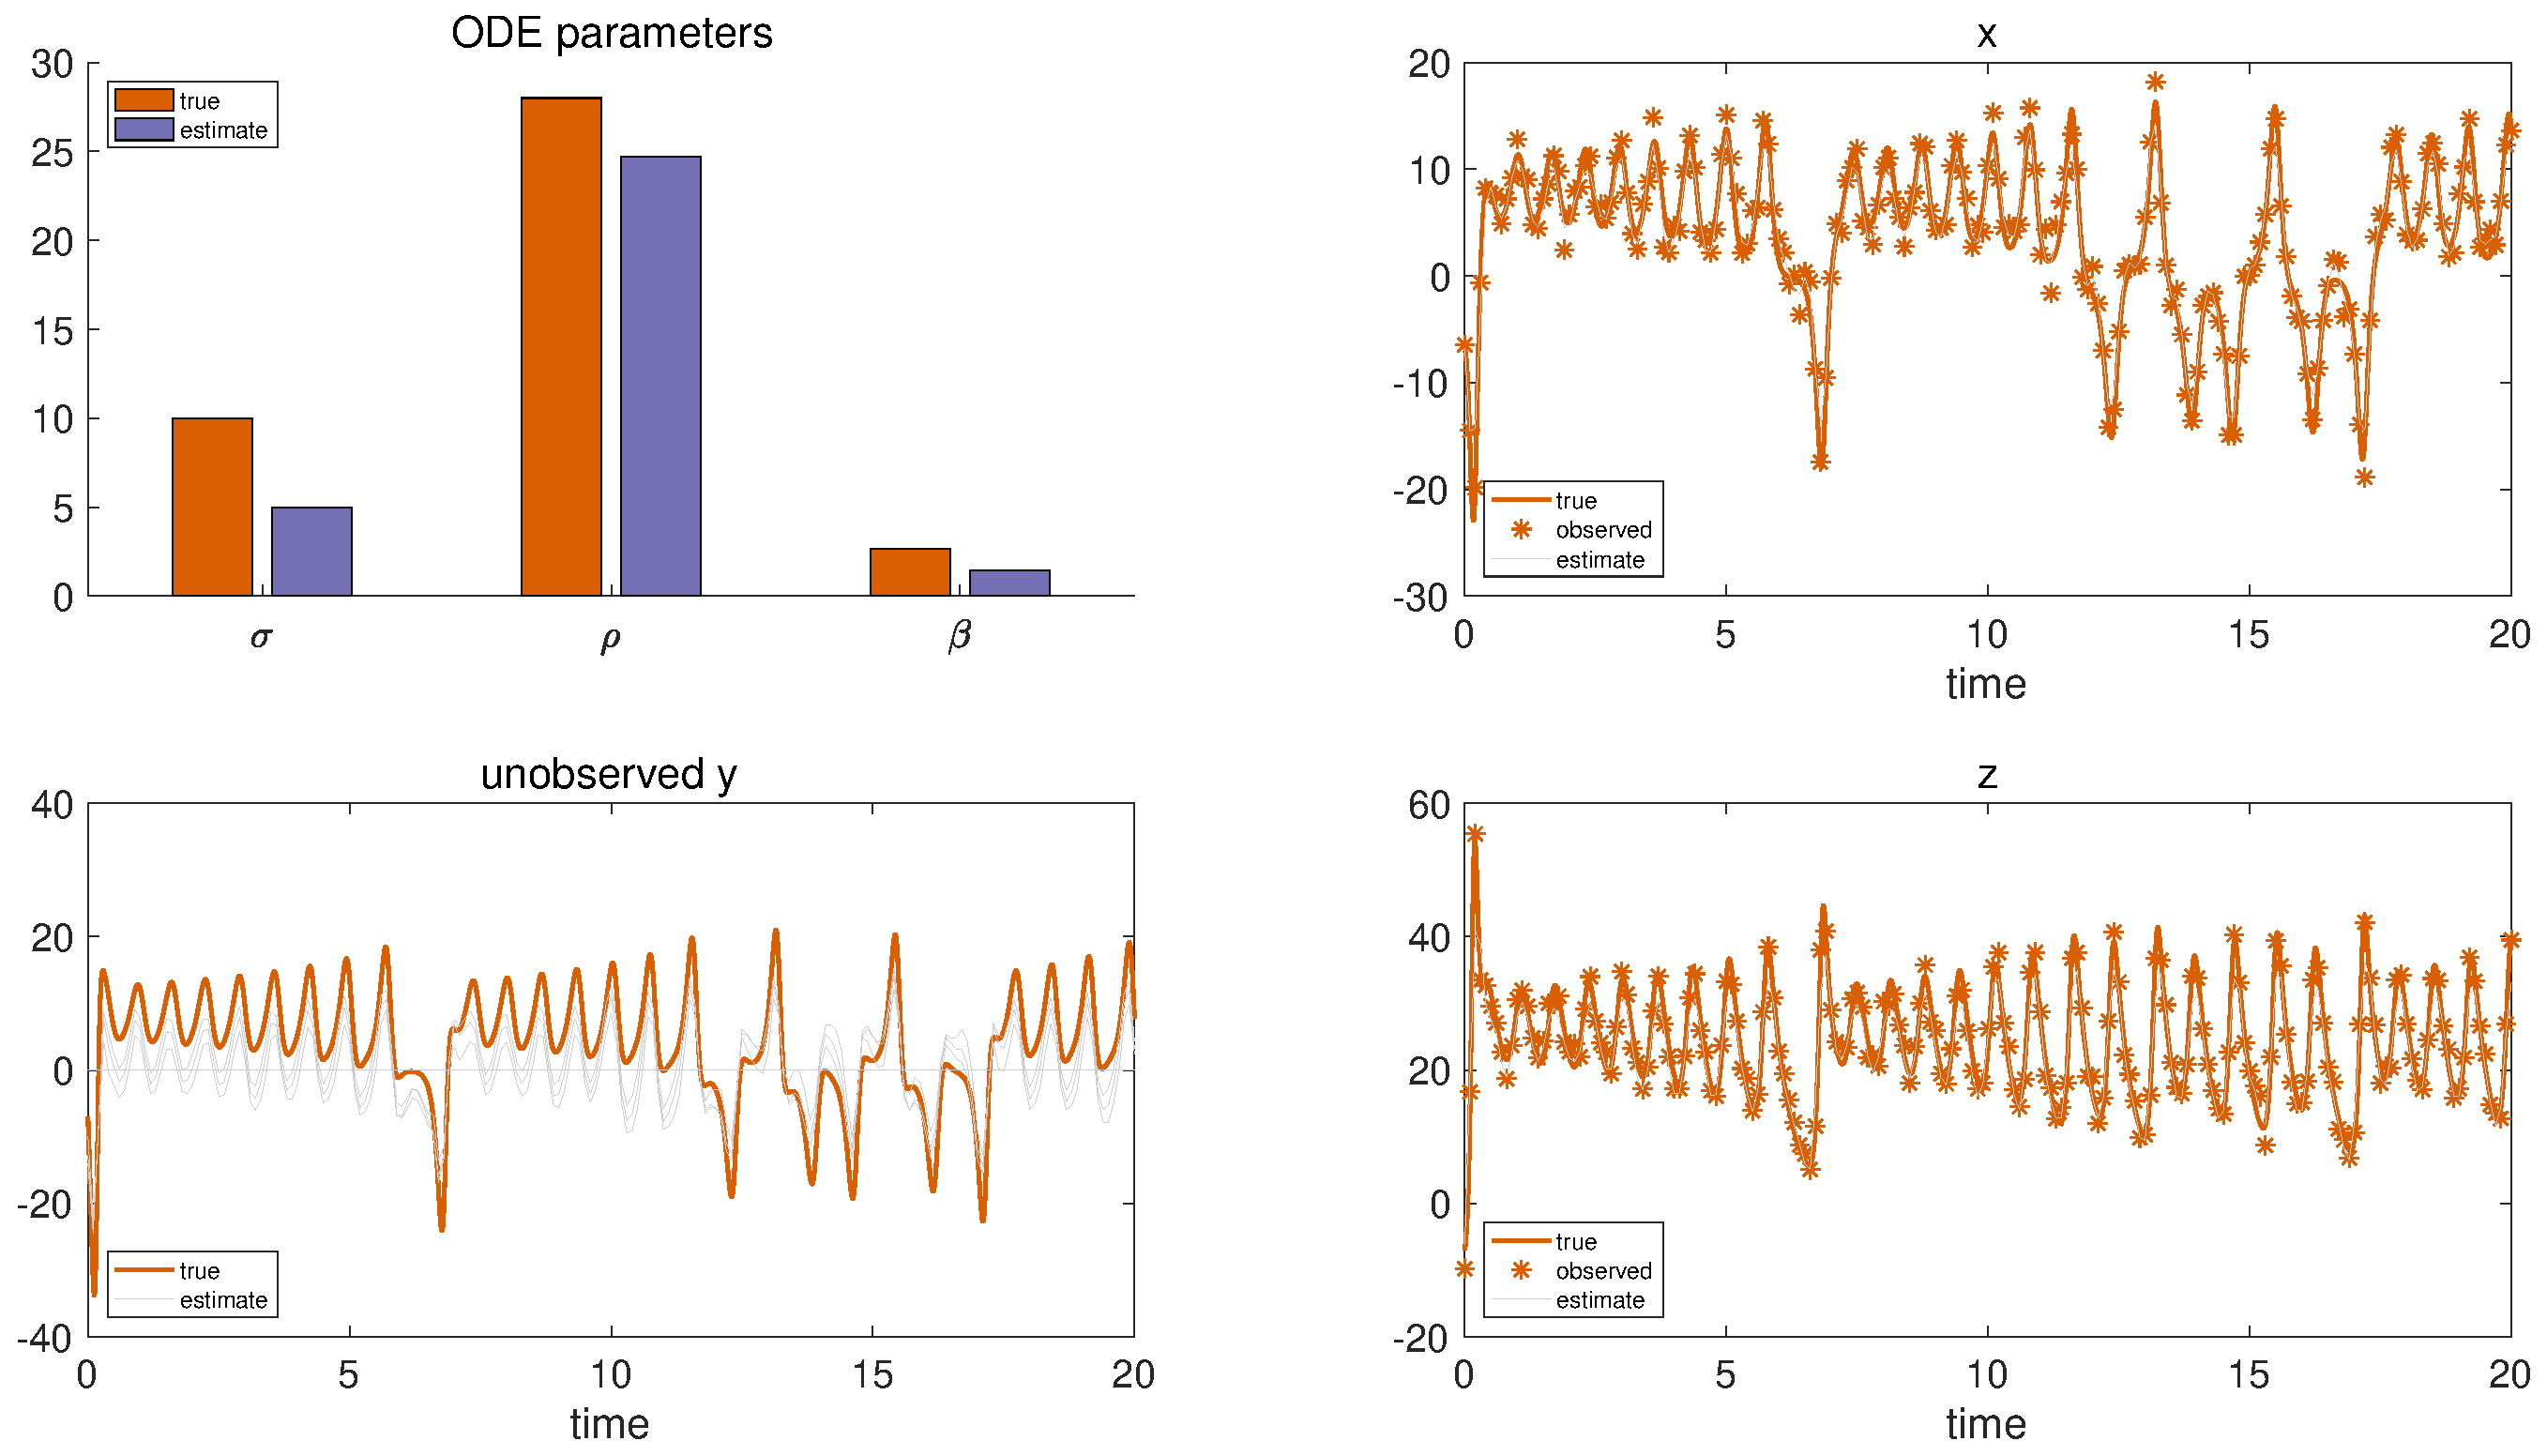
\includegraphics [width=4in]{Lorenz_attractor_4_08.eps}

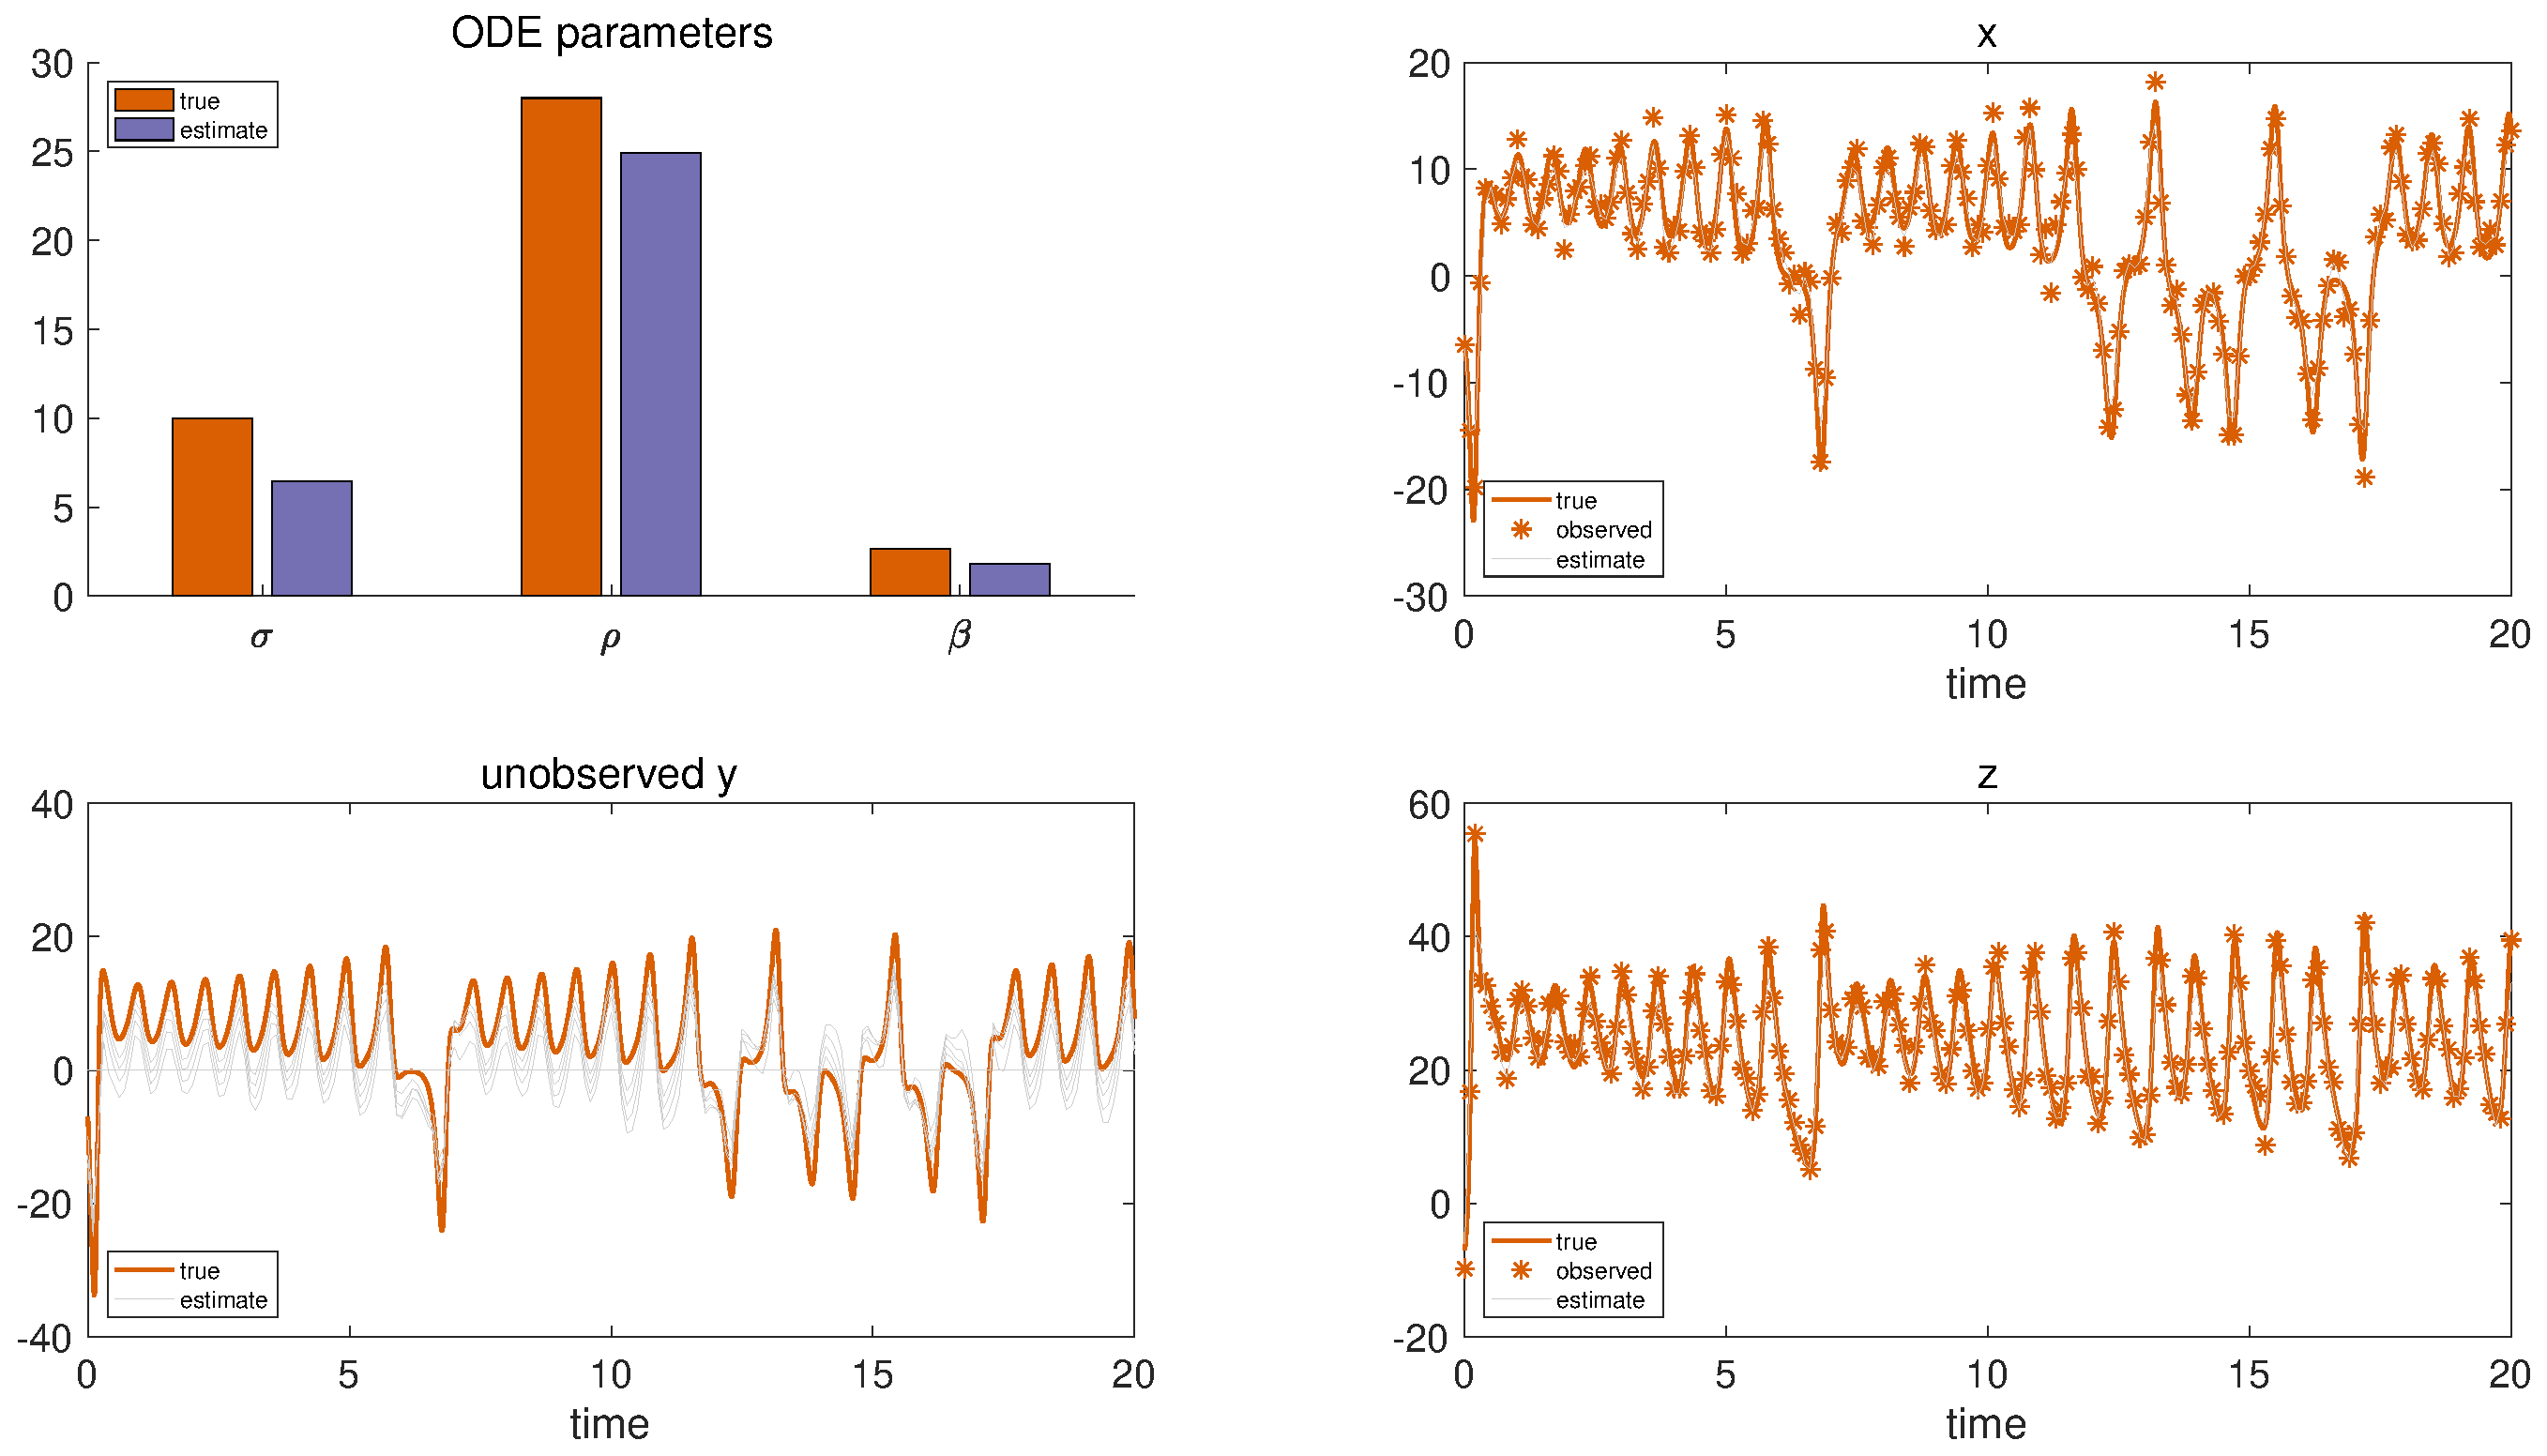
\includegraphics [width=4in]{Lorenz_attractor_4_09.eps}

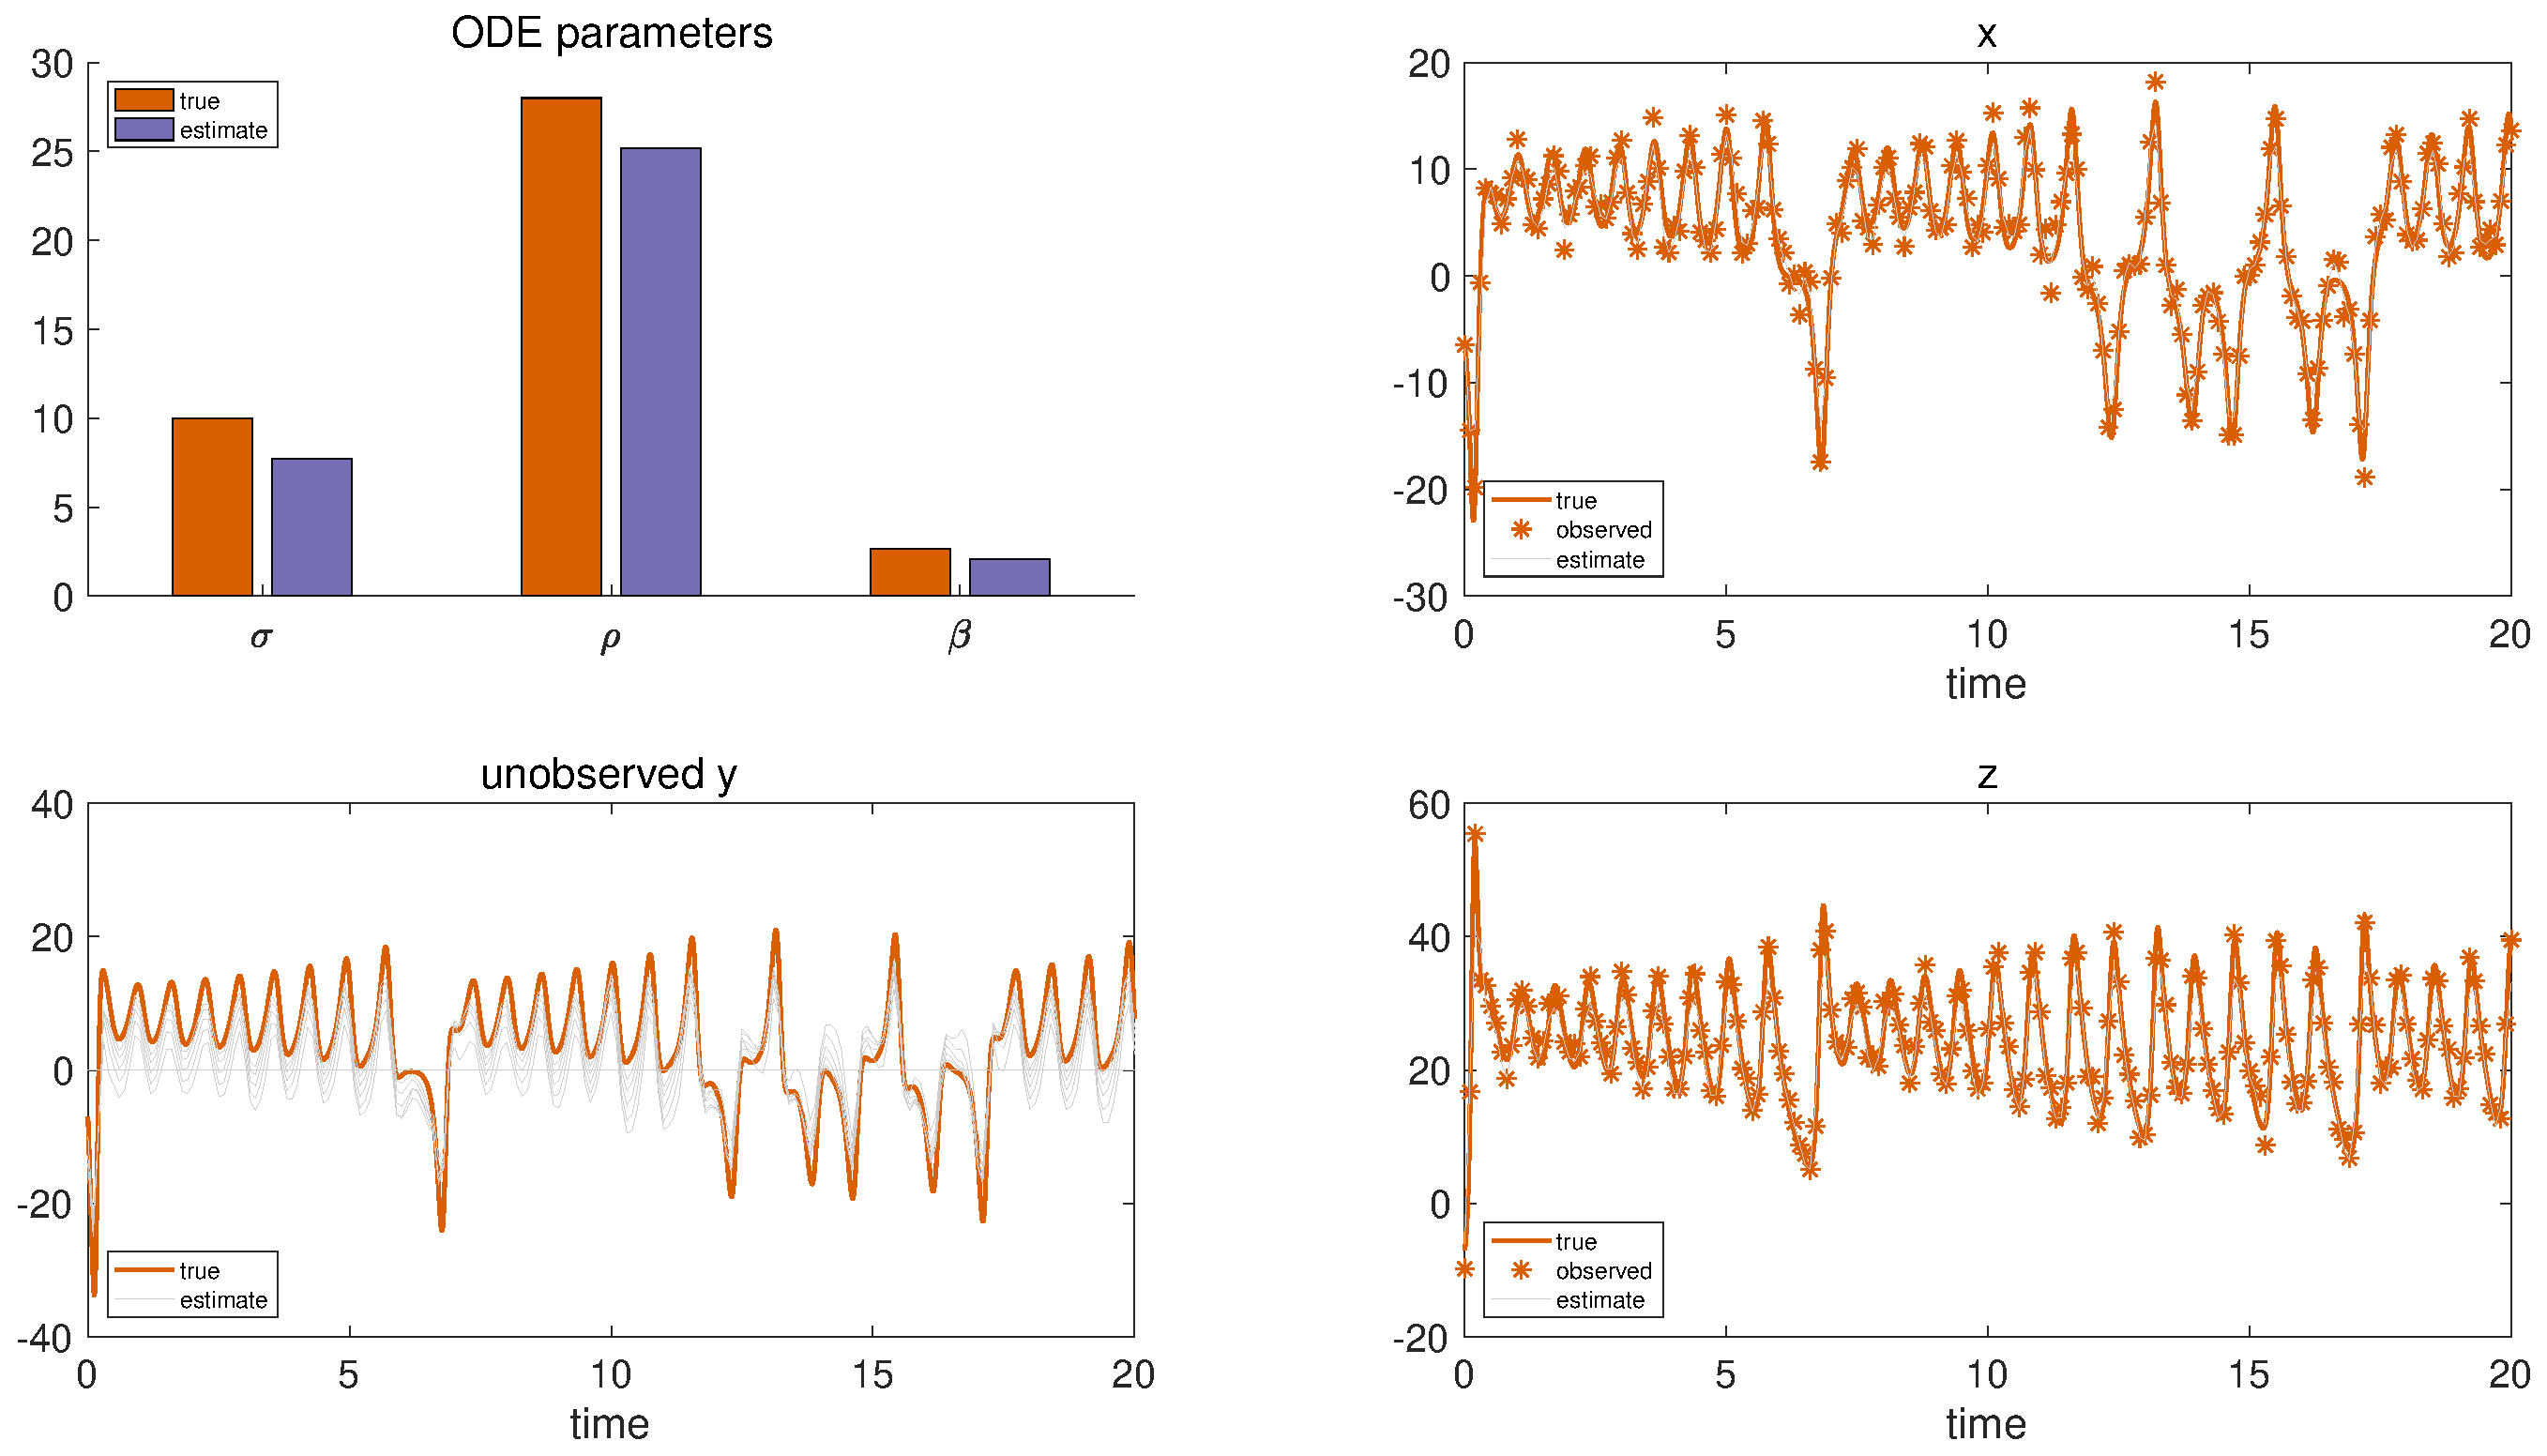
\includegraphics [width=4in]{Lorenz_attractor_4_10.eps}

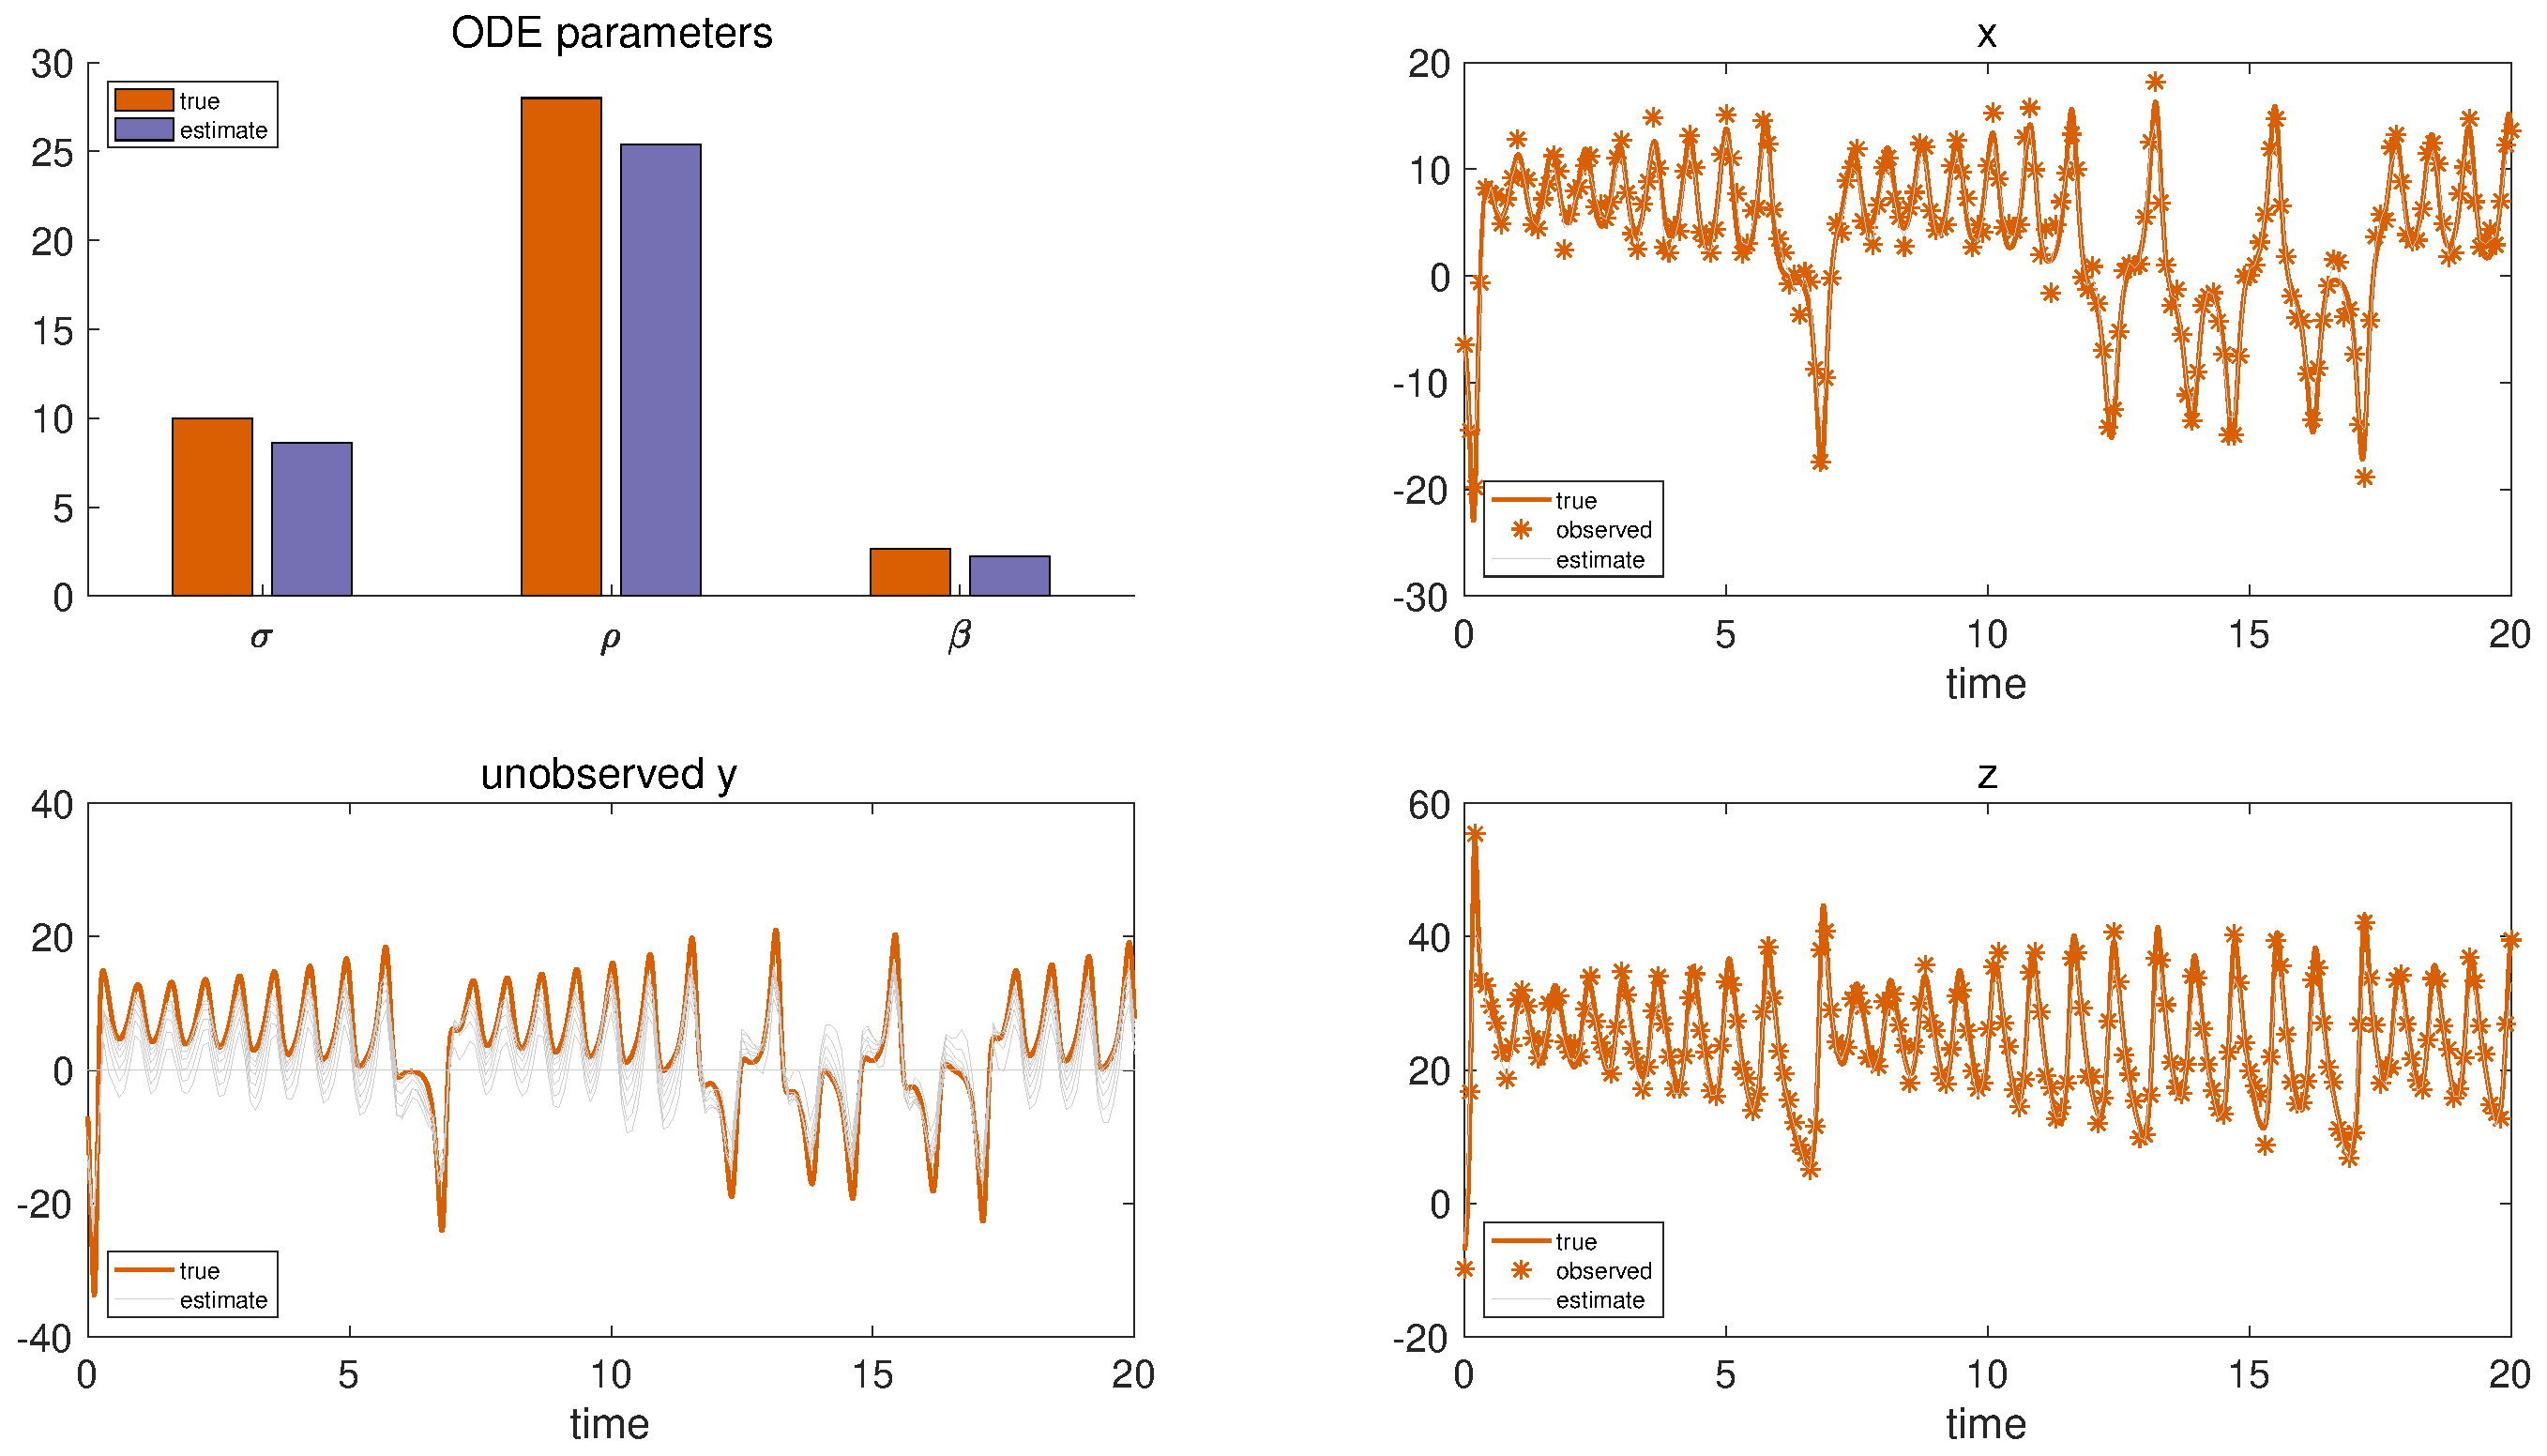
\includegraphics [width=4in]{Lorenz_attractor_4_11.eps}

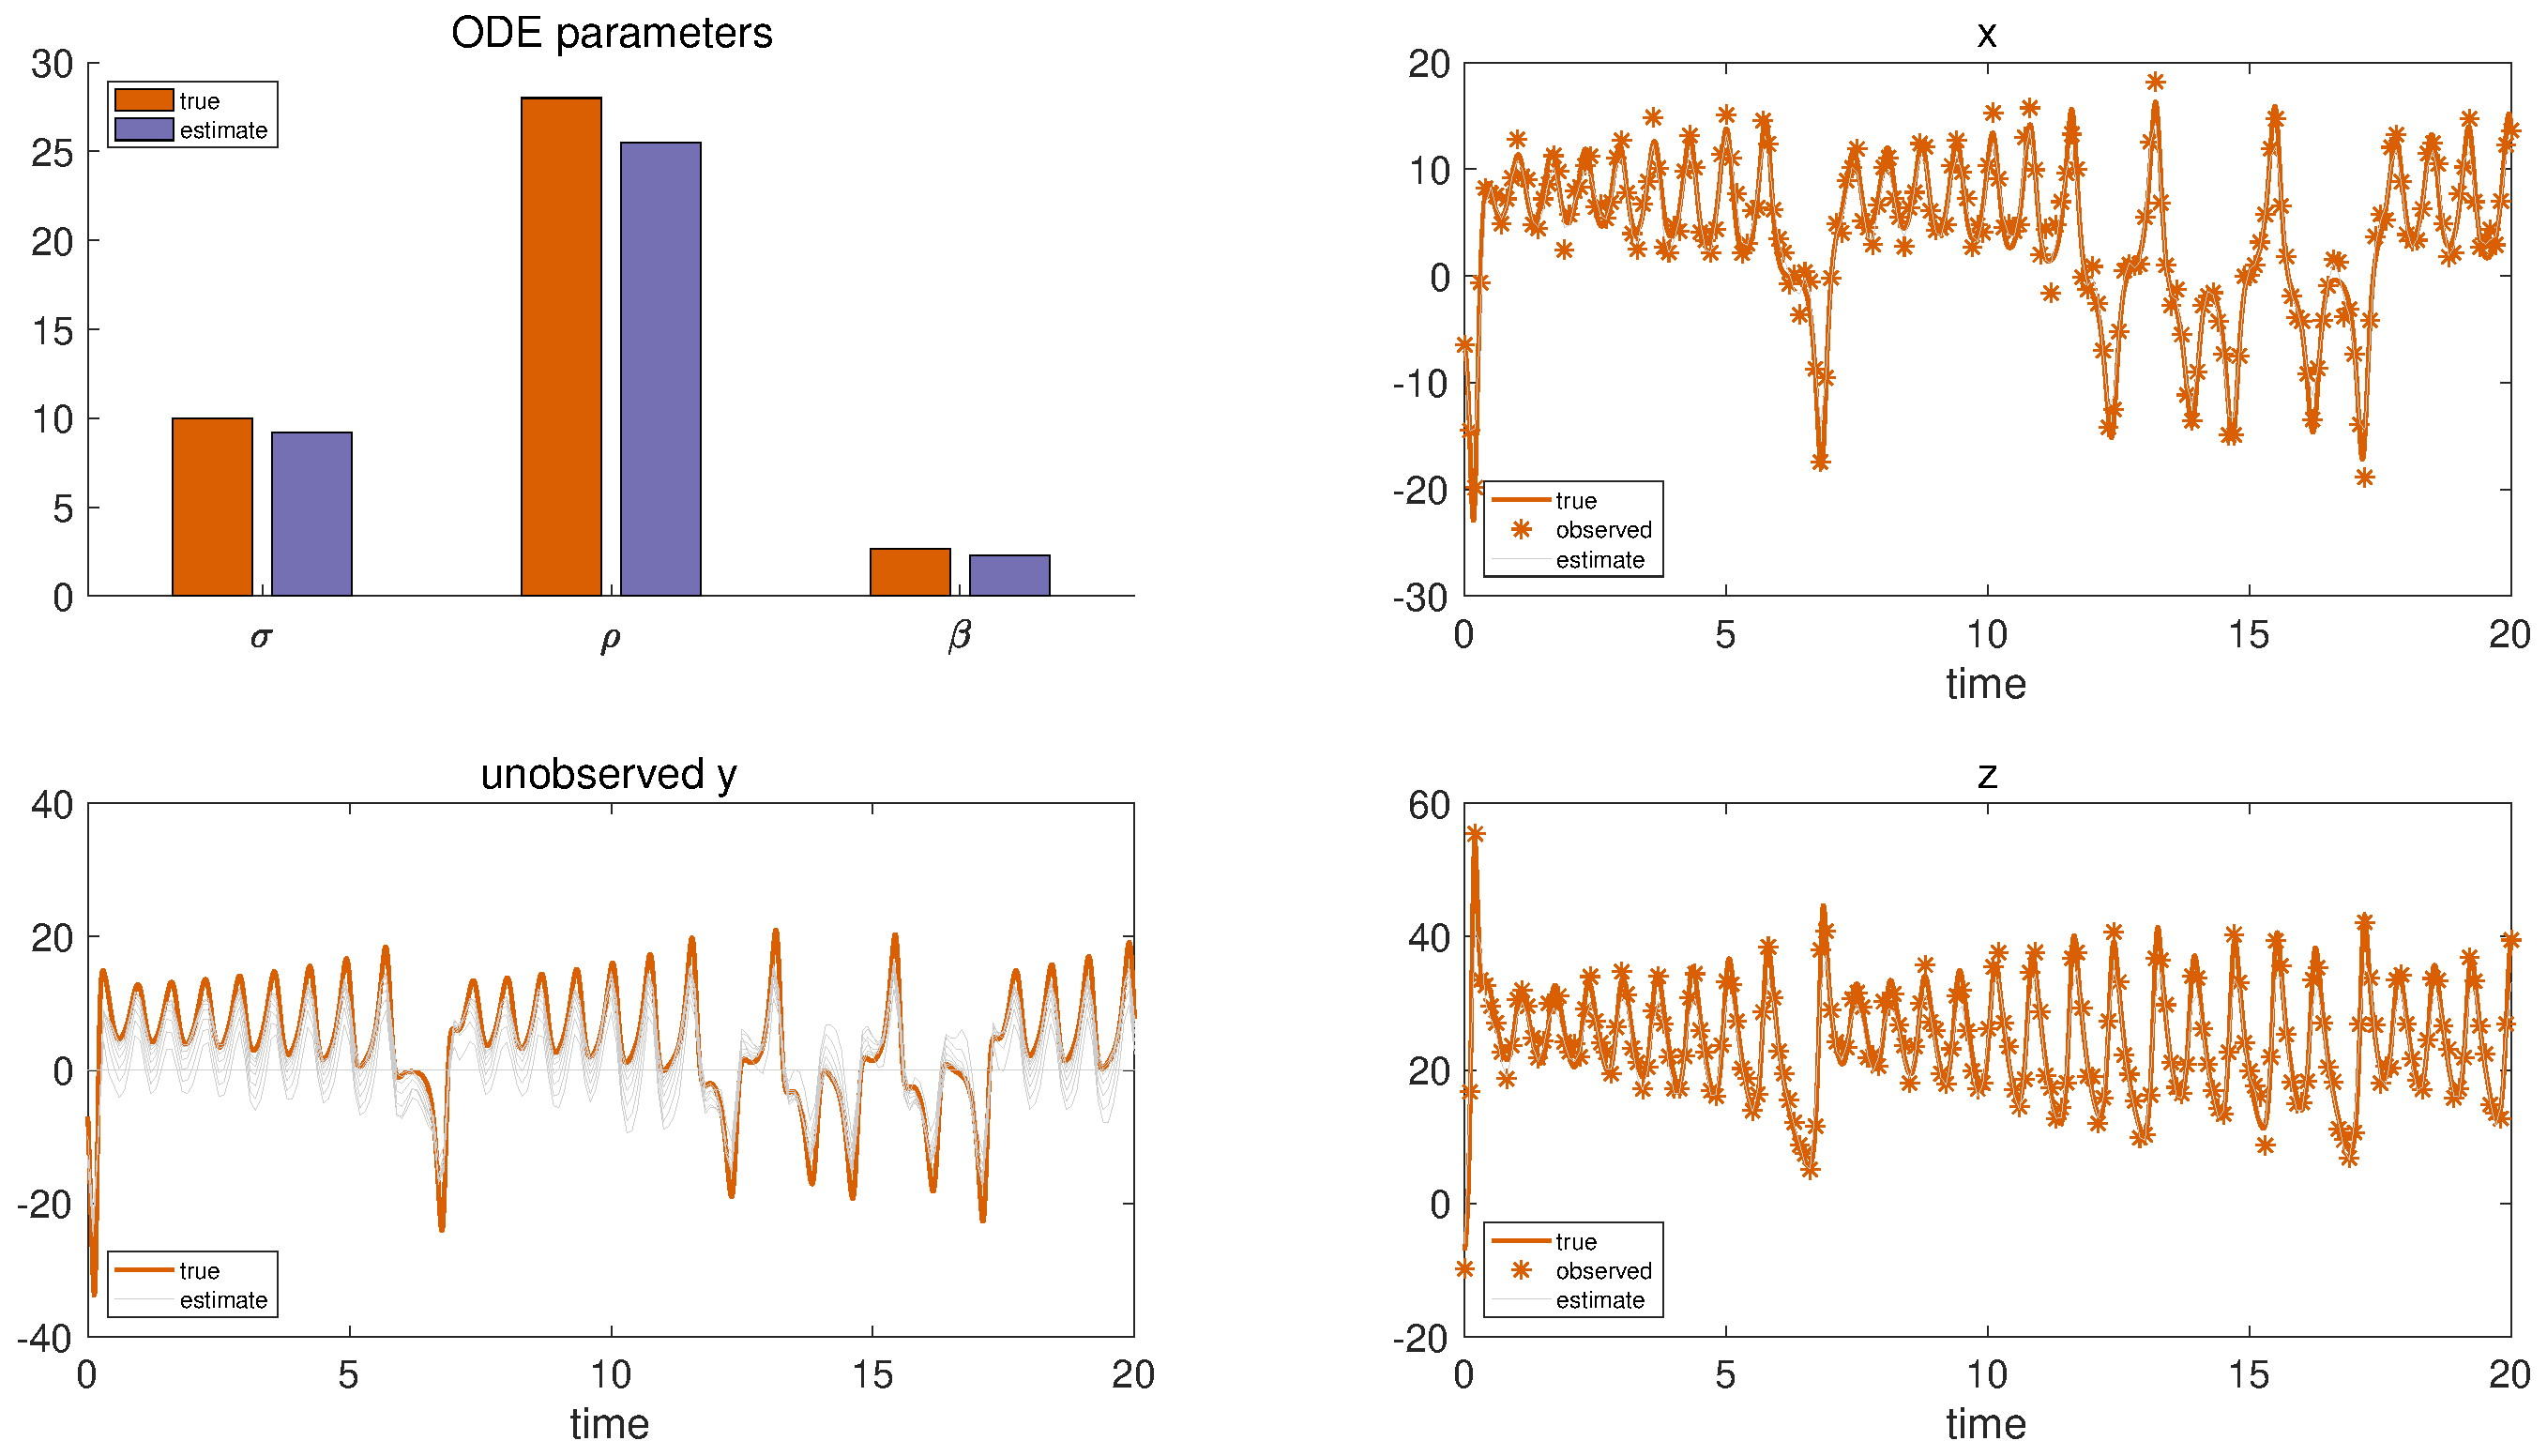
\includegraphics [width=4in]{Lorenz_attractor_4_12.eps}

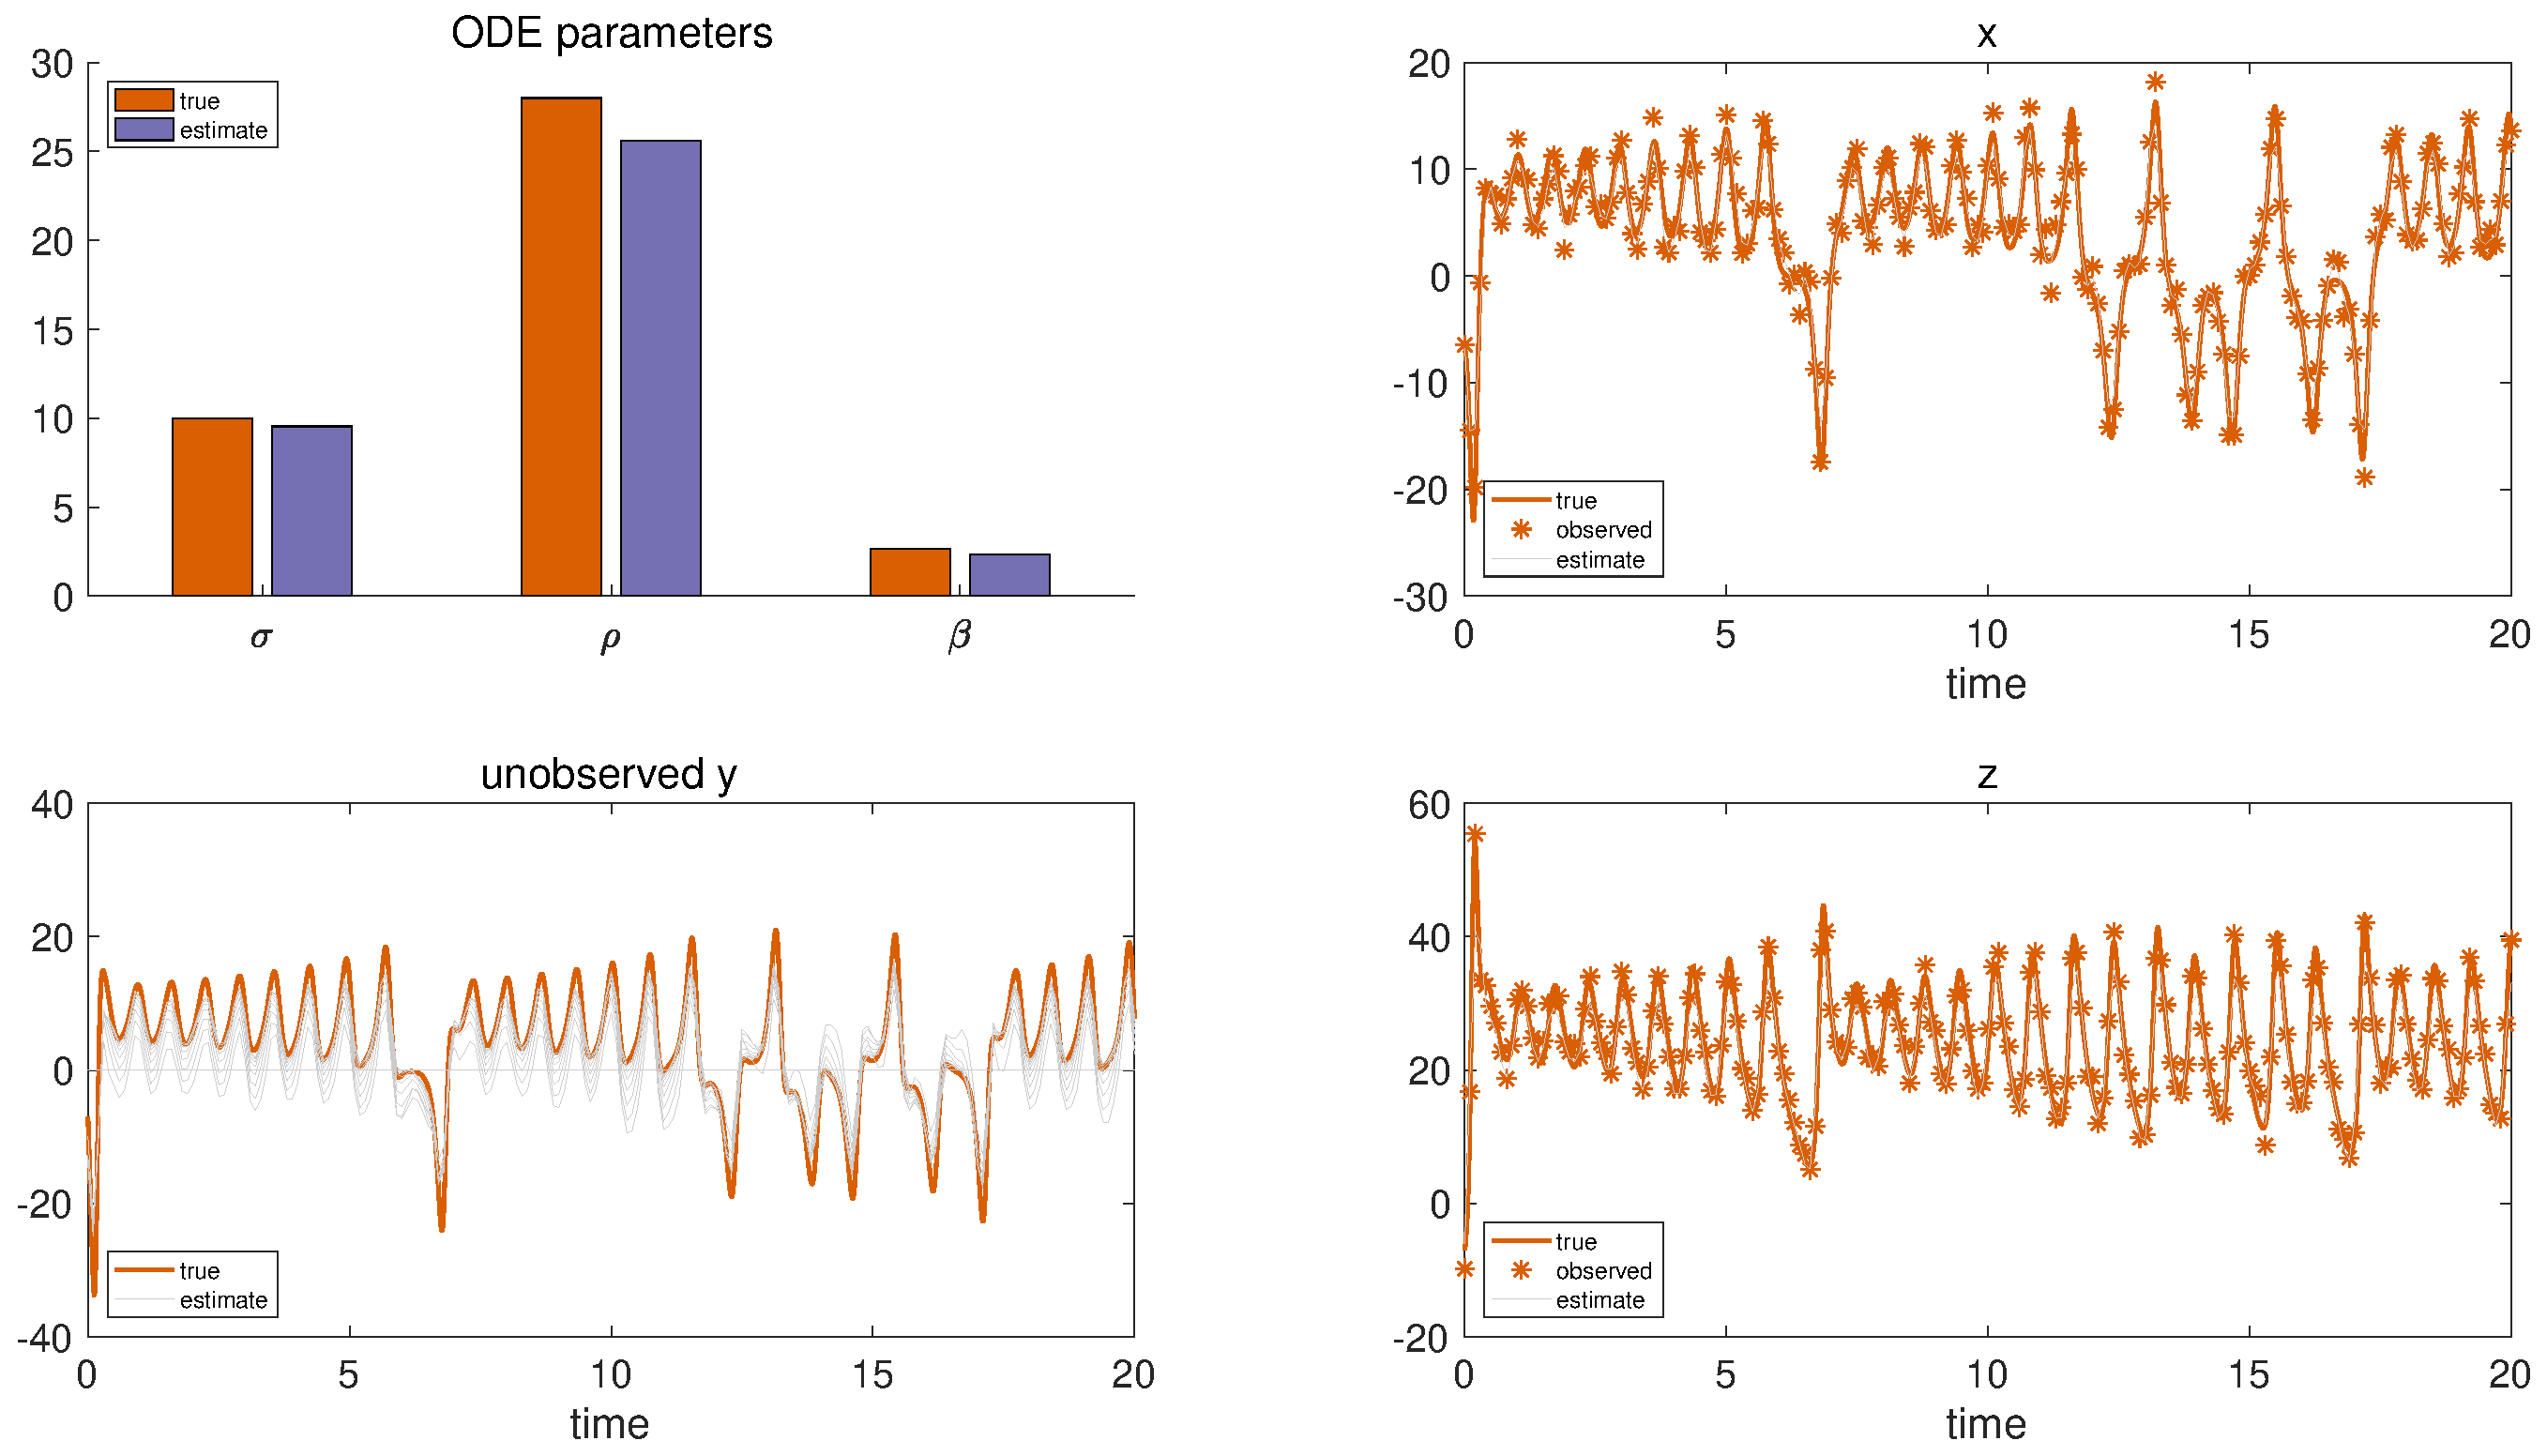
\includegraphics [width=4in]{Lorenz_attractor_4_13.eps}

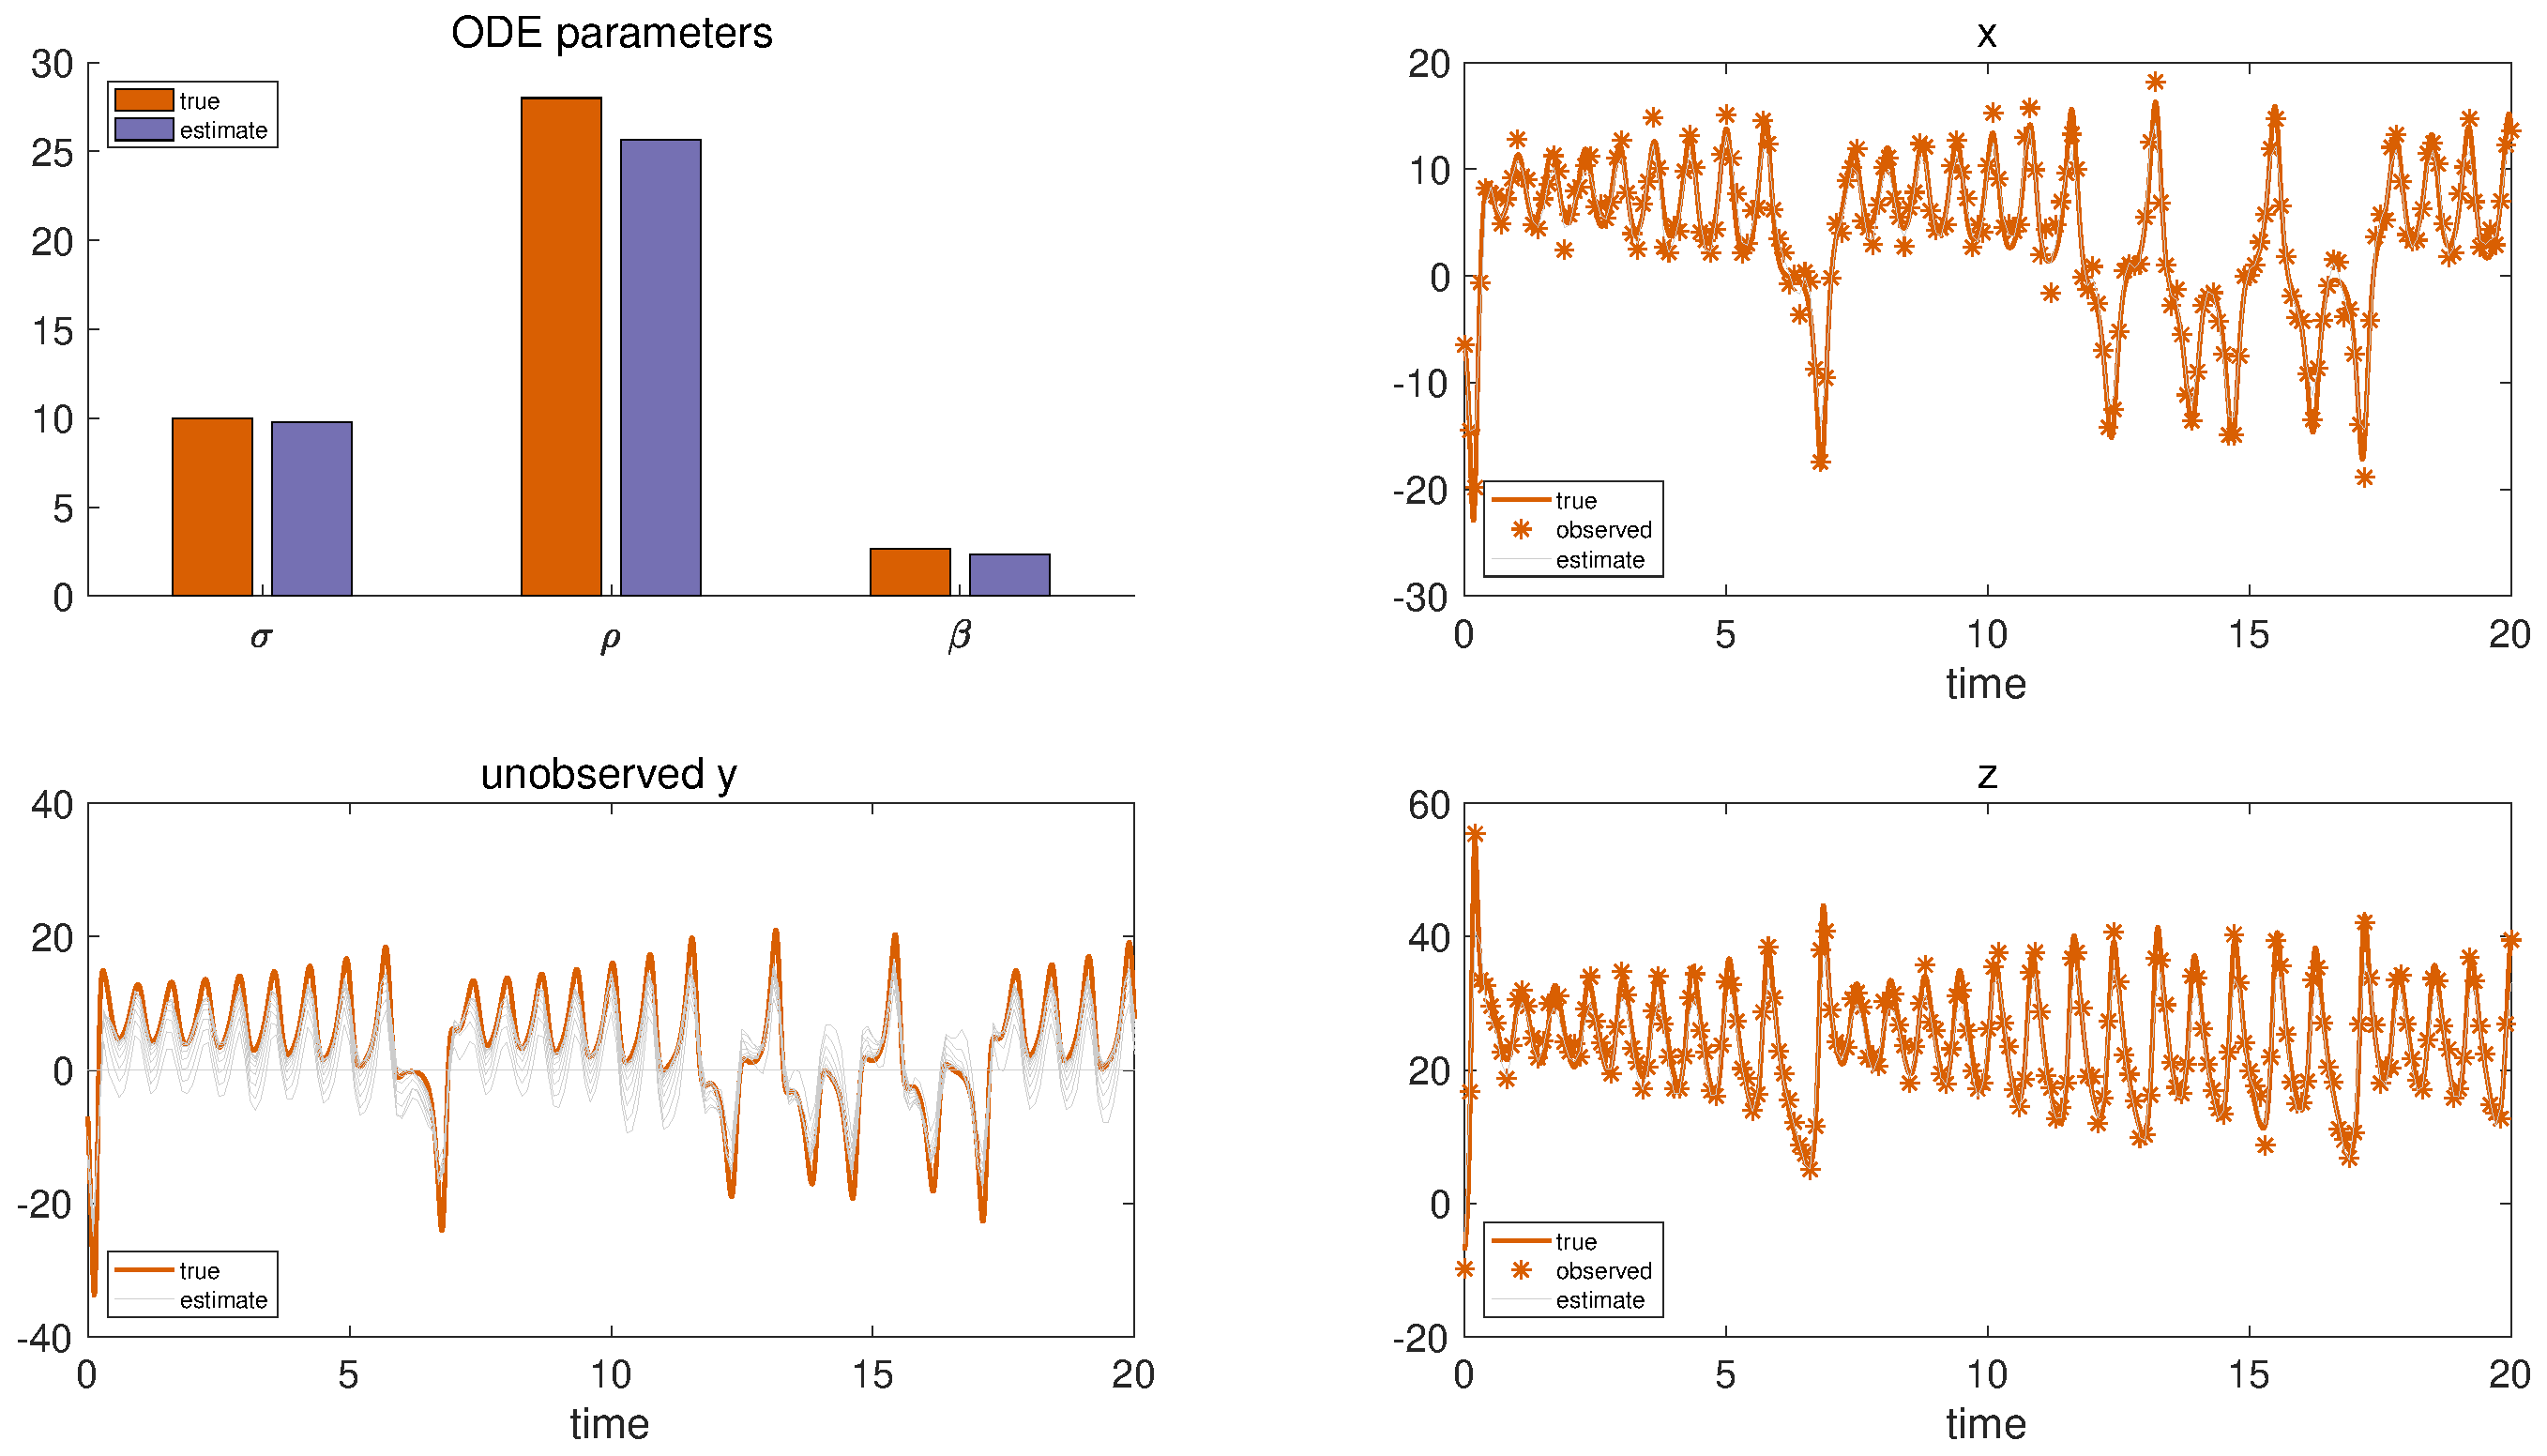
\includegraphics [width=4in]{Lorenz_attractor_4_14.eps}

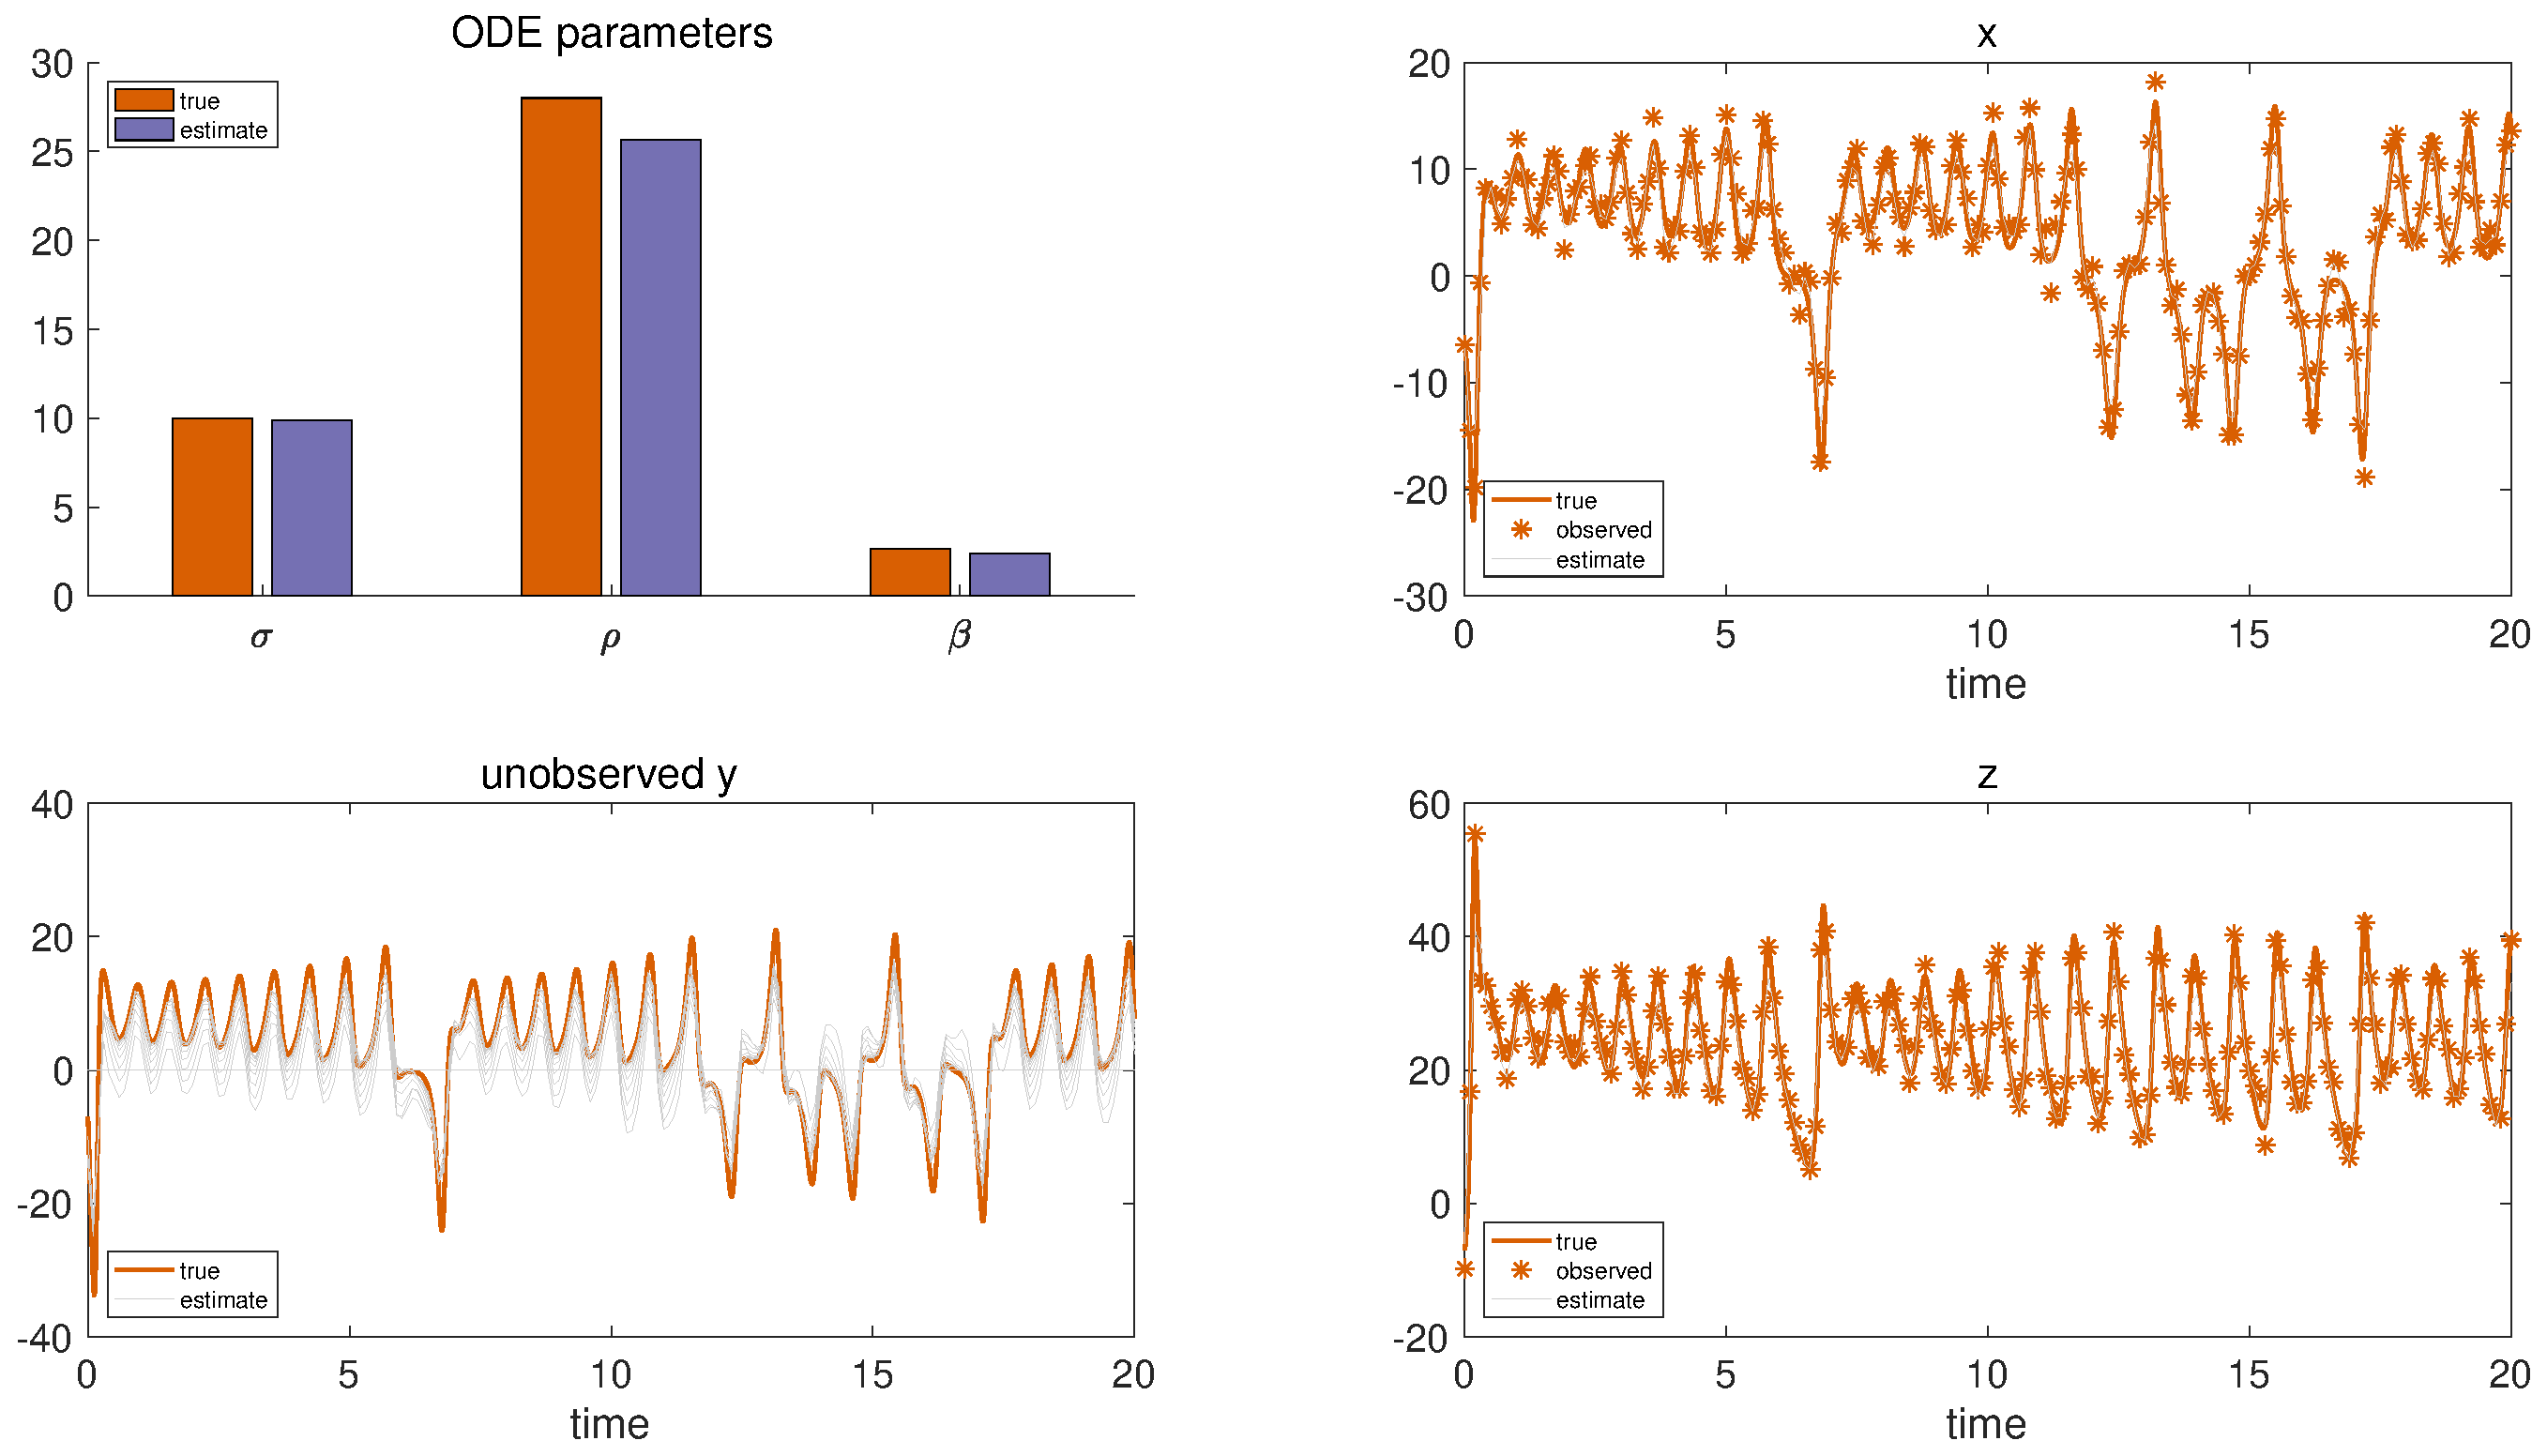
\includegraphics [width=4in]{Lorenz_attractor_4_15.eps}

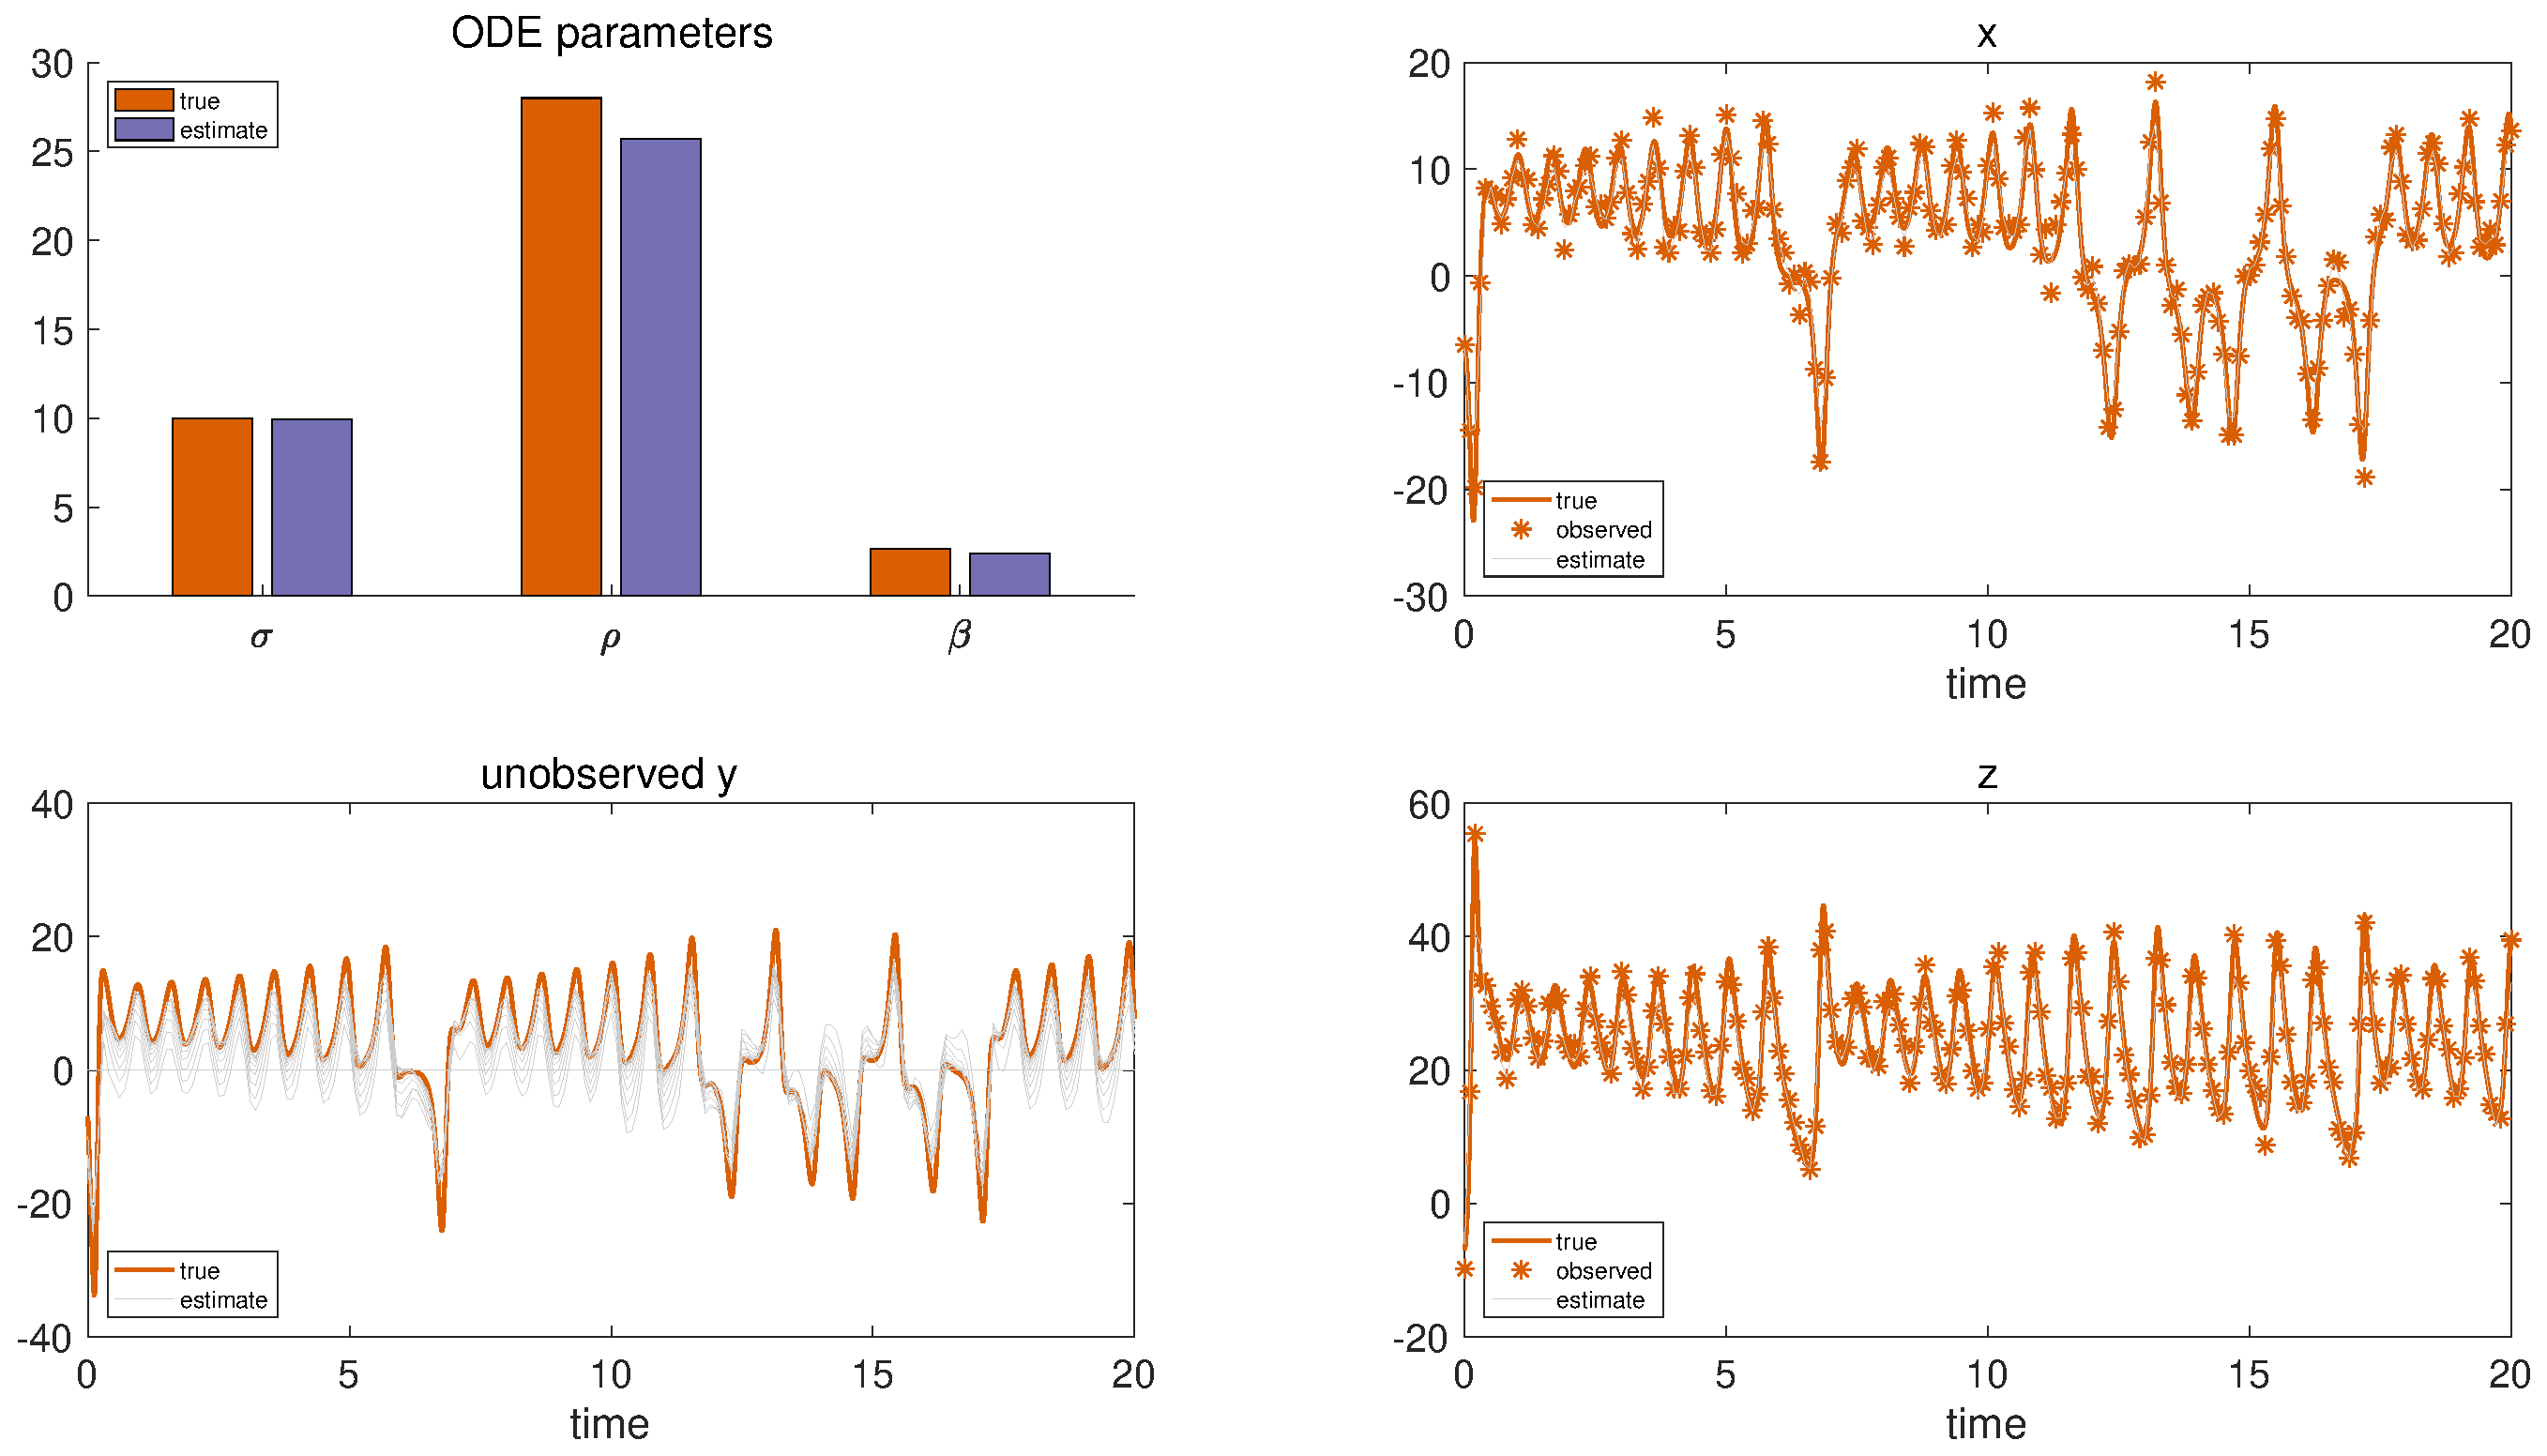
\includegraphics [width=4in]{Lorenz_attractor_4_16.eps}

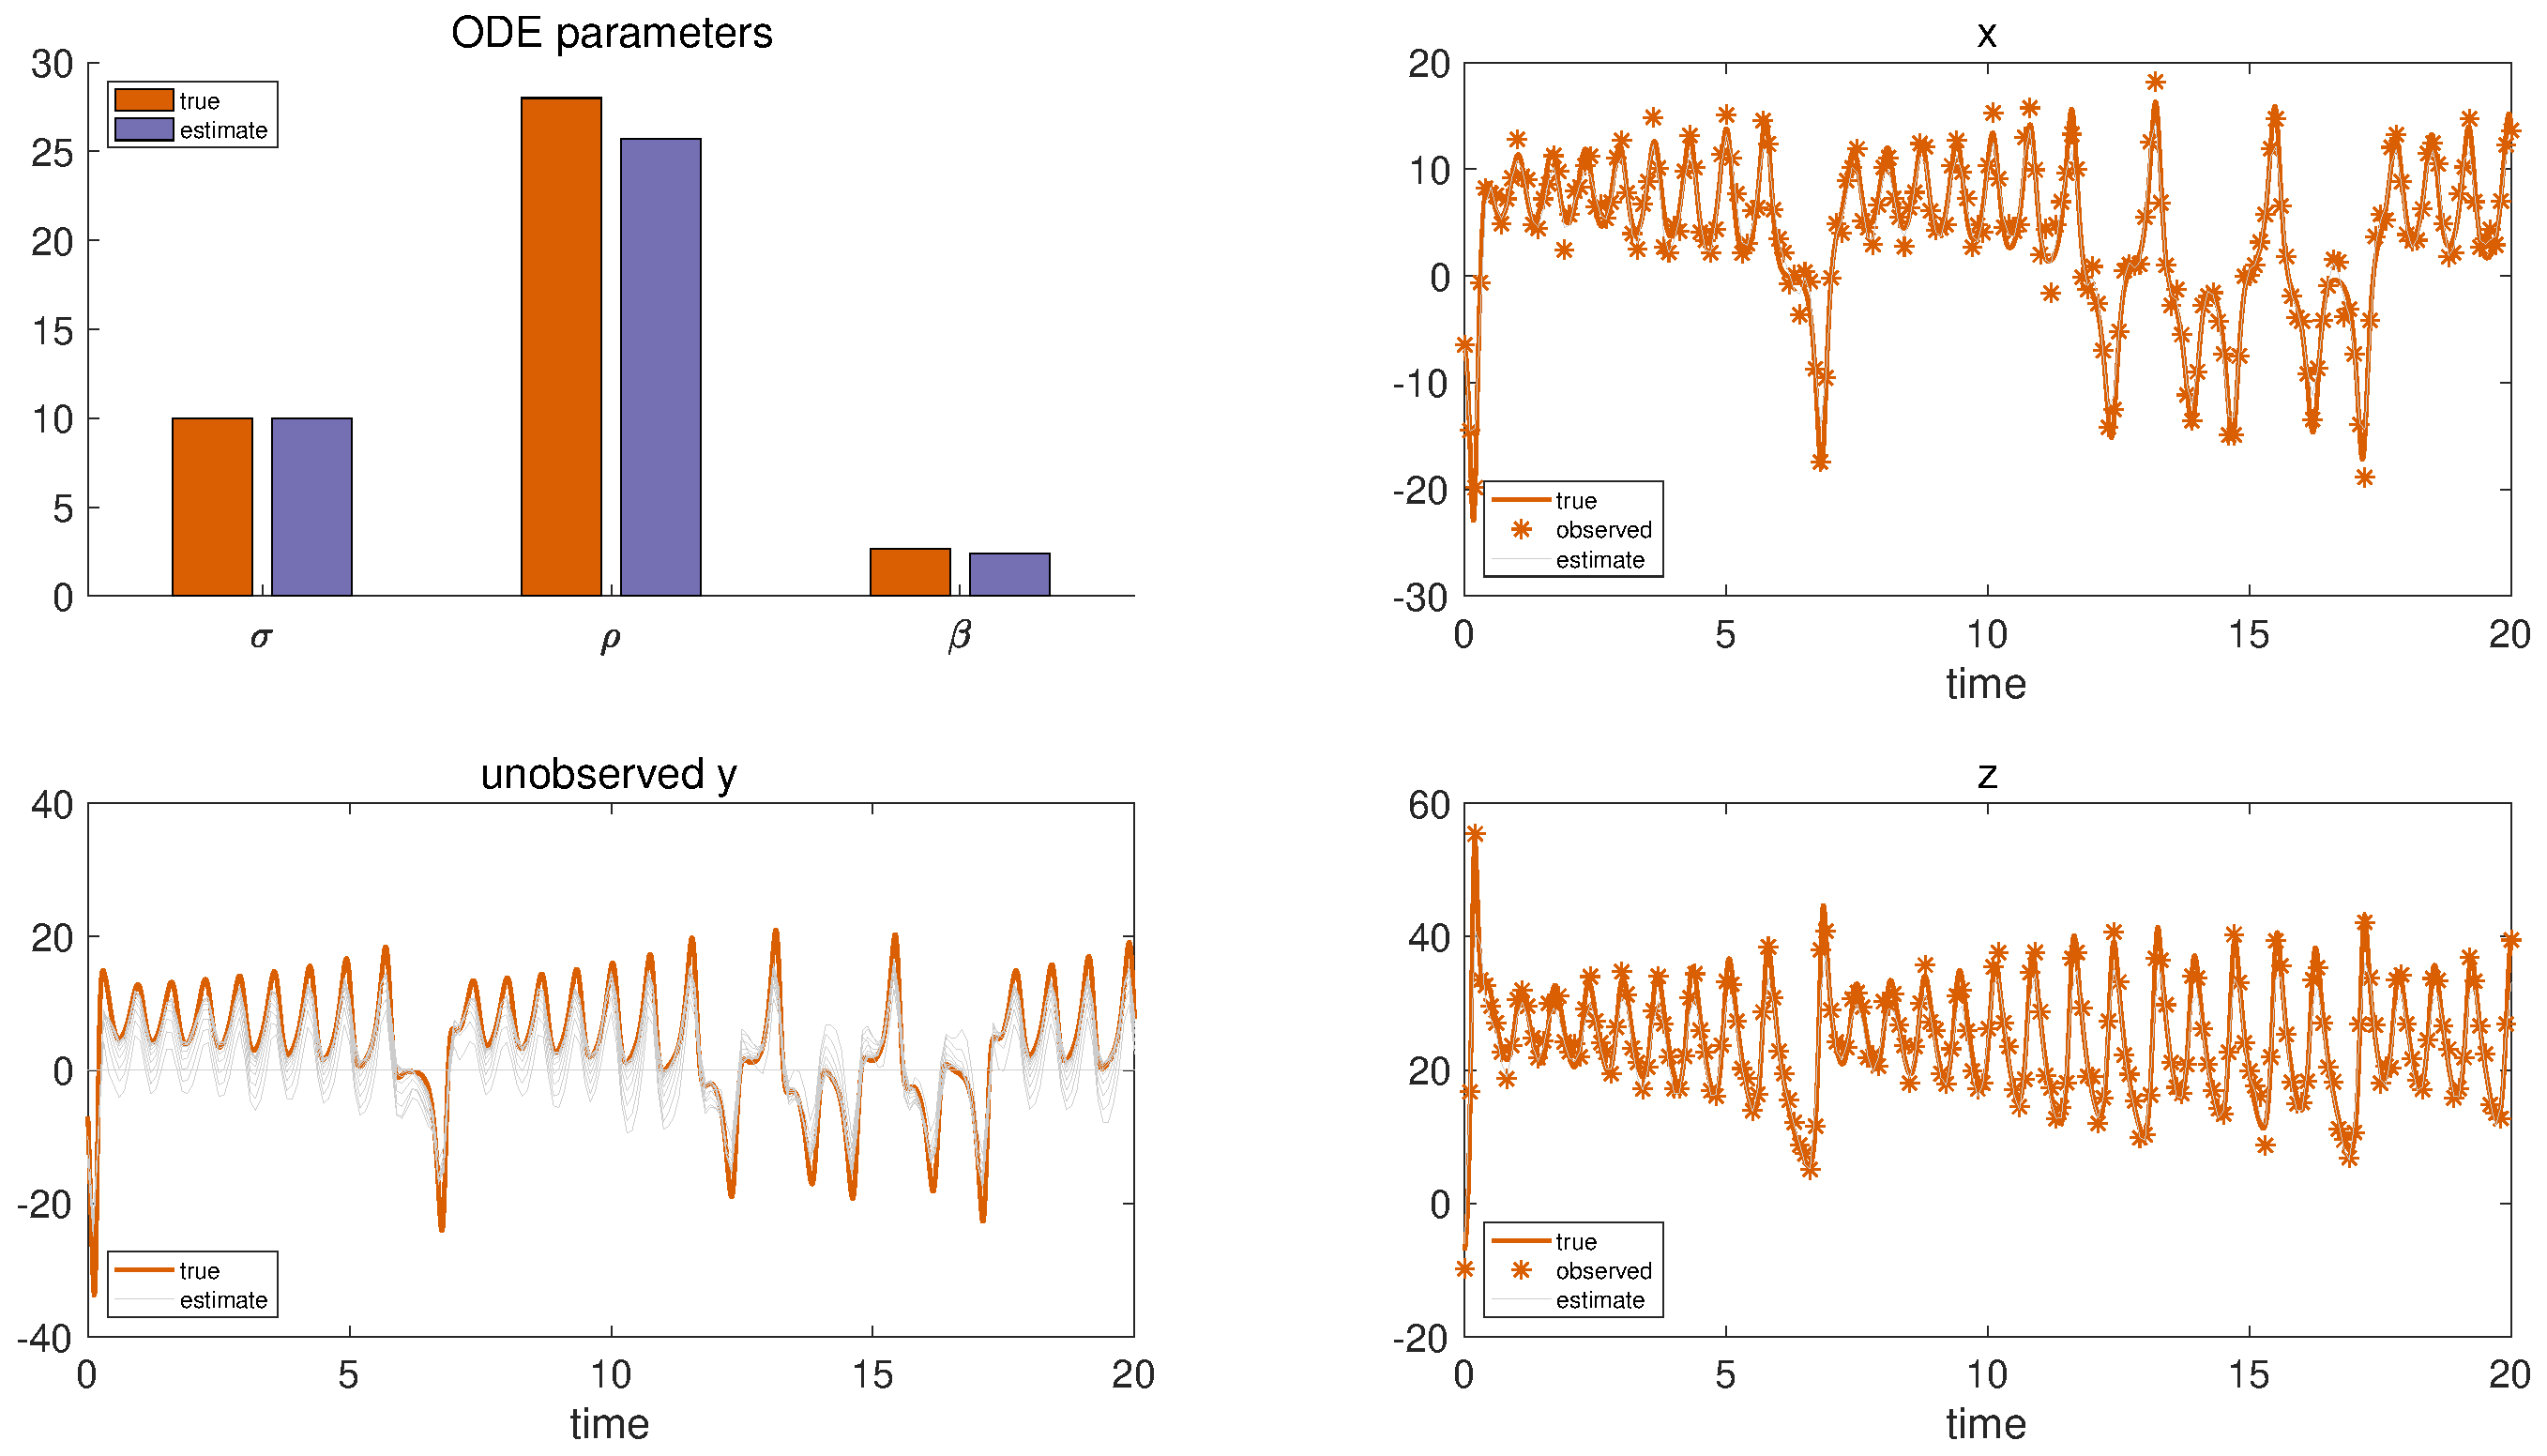
\includegraphics [width=4in]{Lorenz_attractor_4_17.eps}

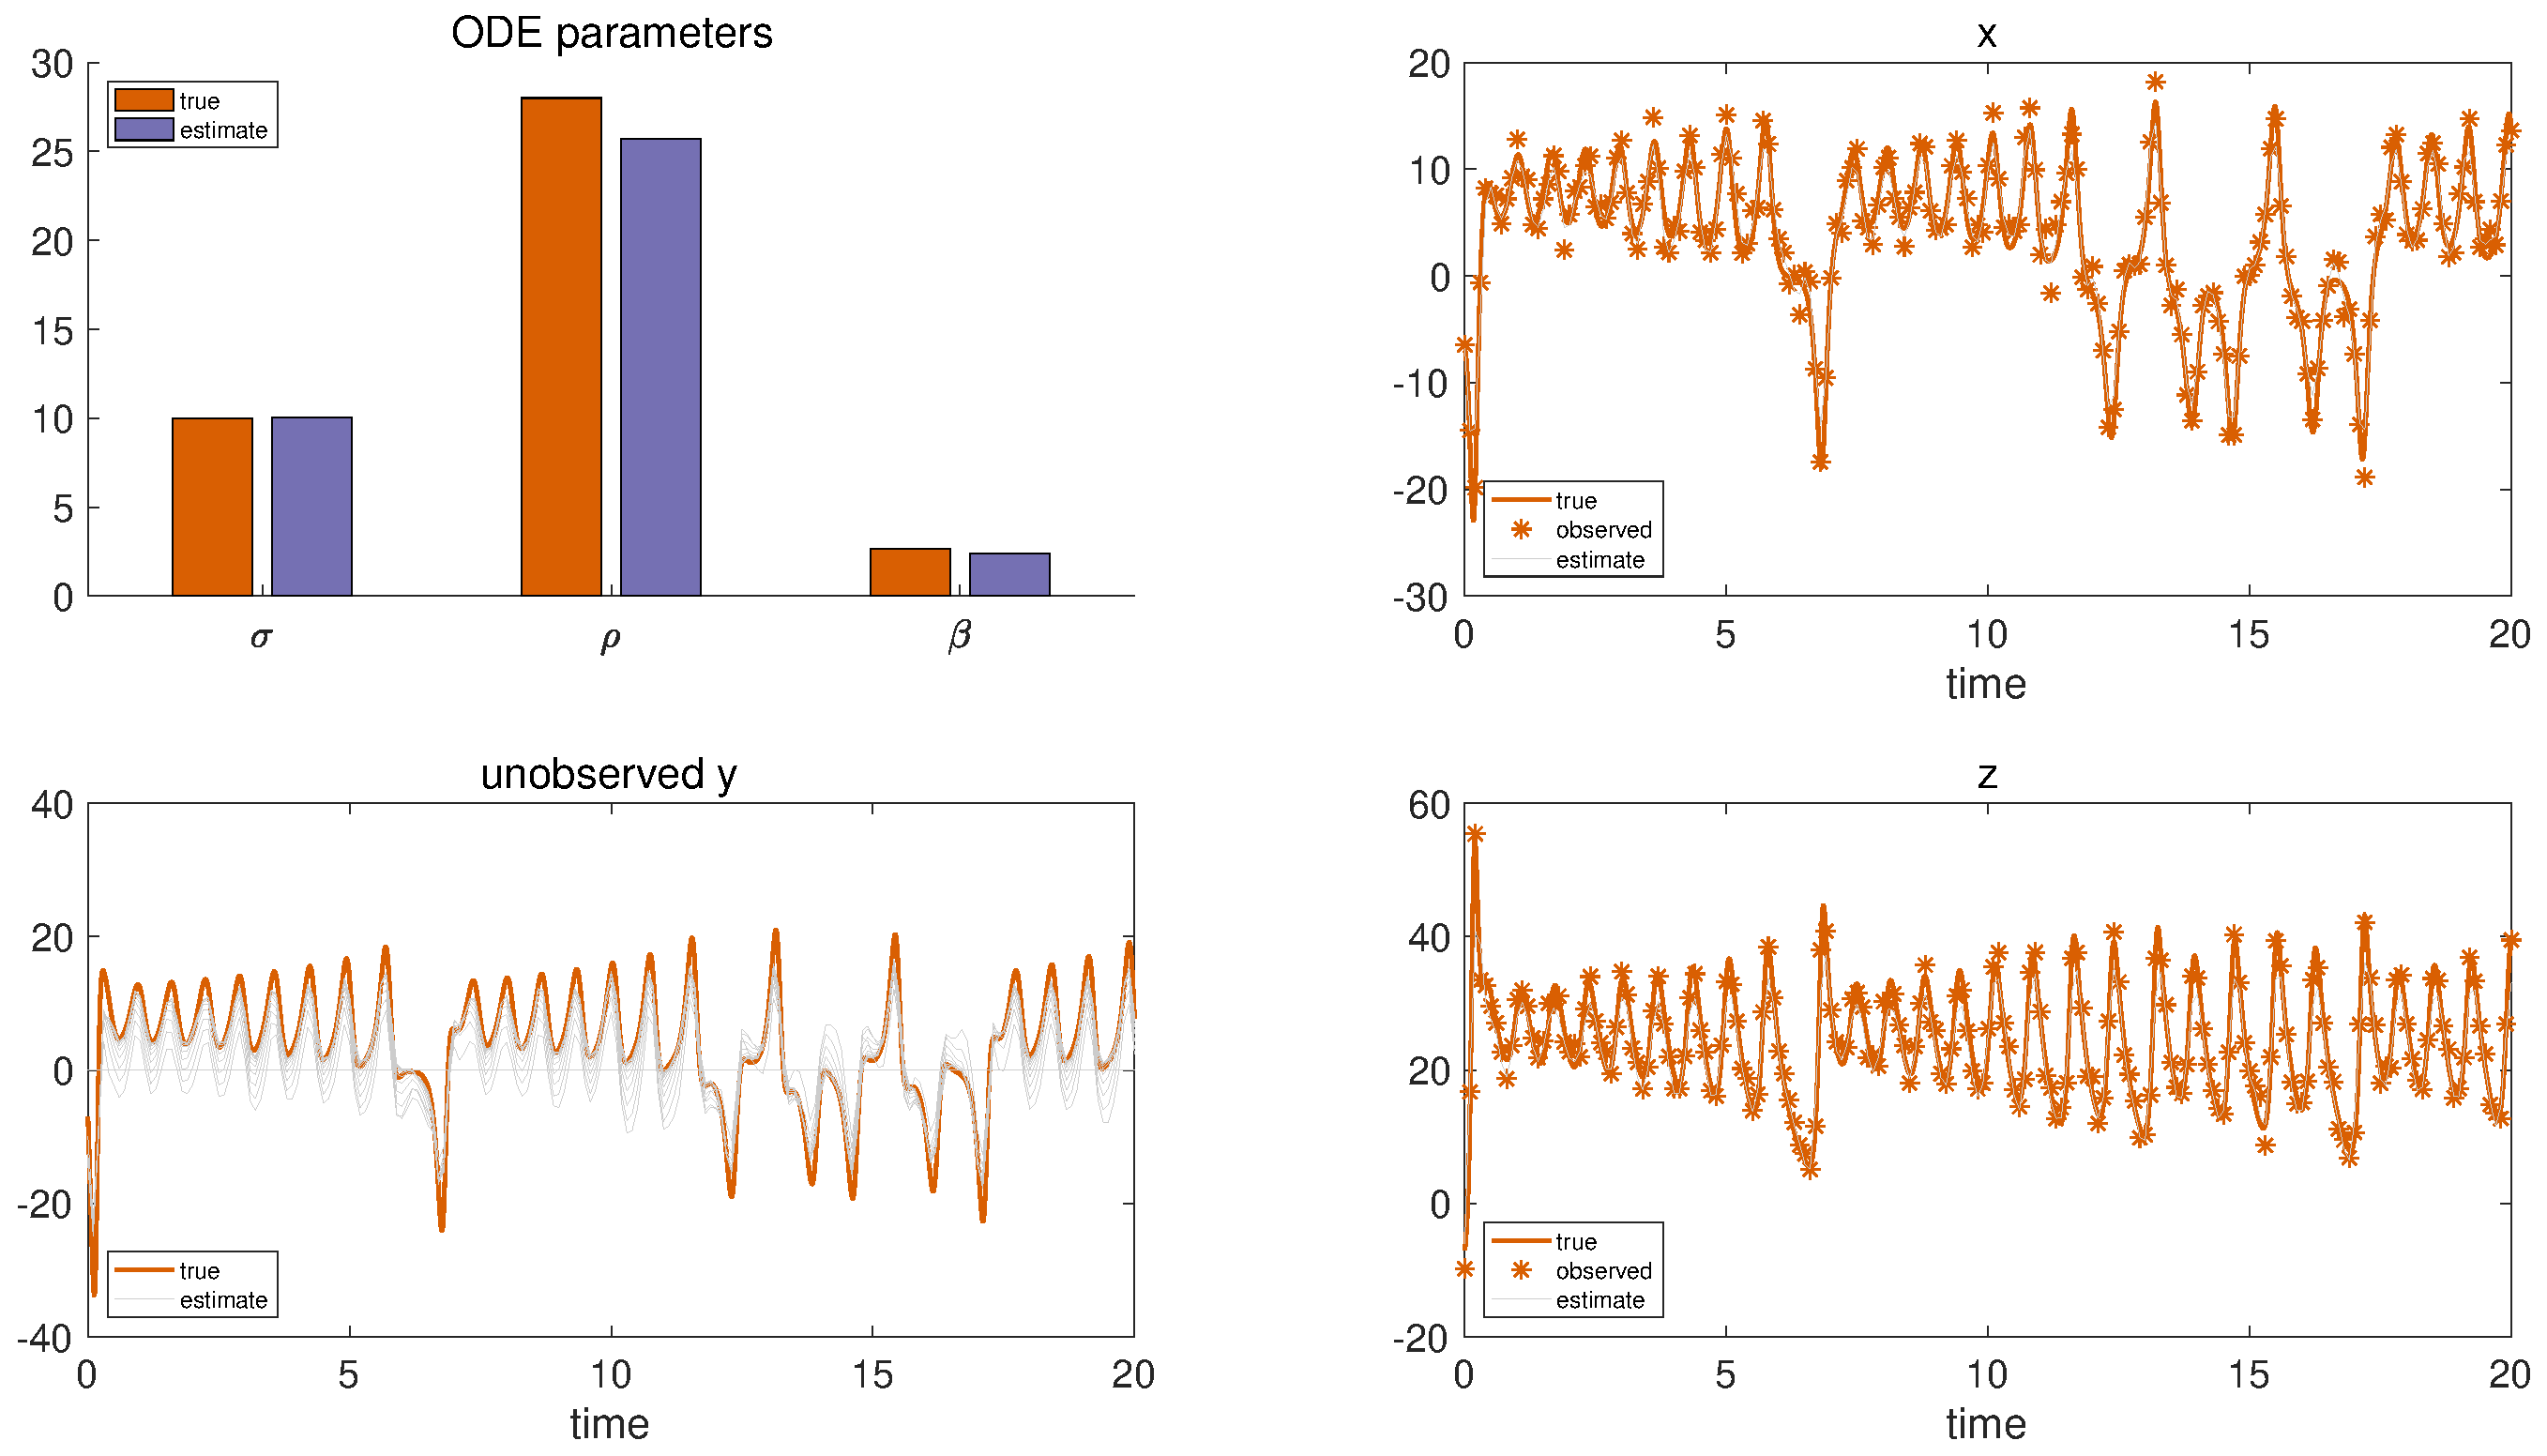
\includegraphics [width=4in]{Lorenz_attractor_4_18.eps}

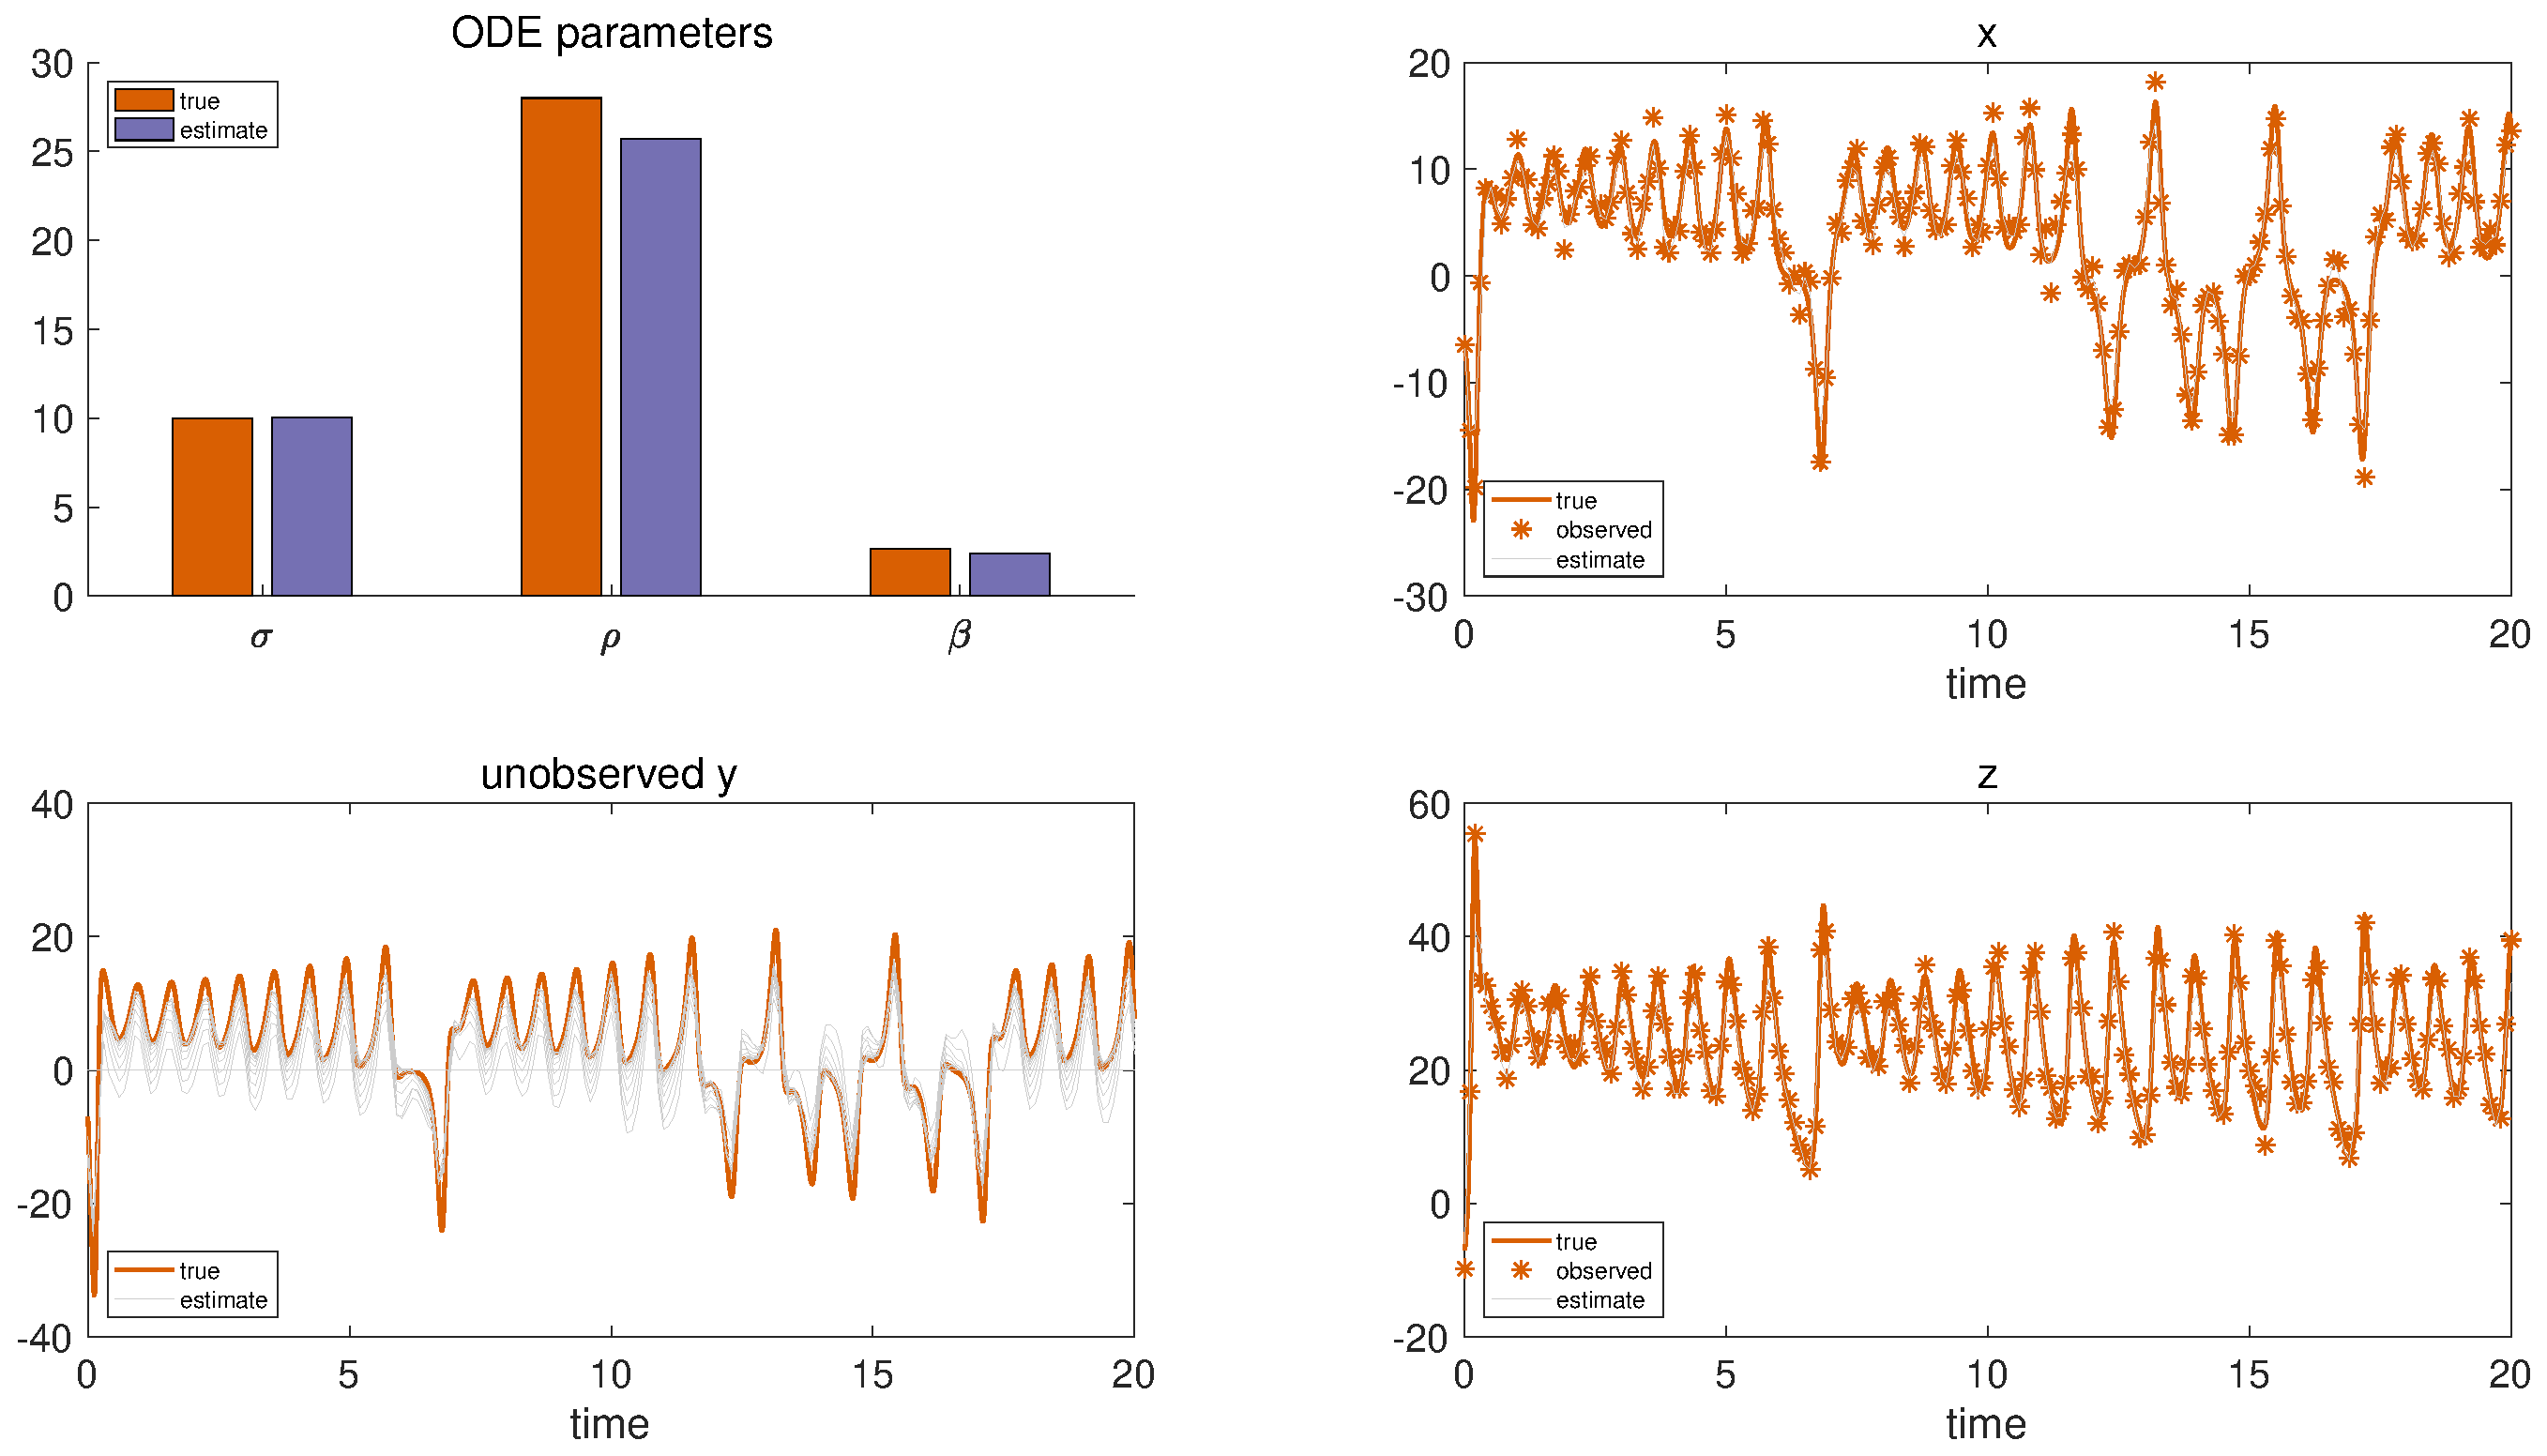
\includegraphics [width=4in]{Lorenz_attractor_4_19.eps}

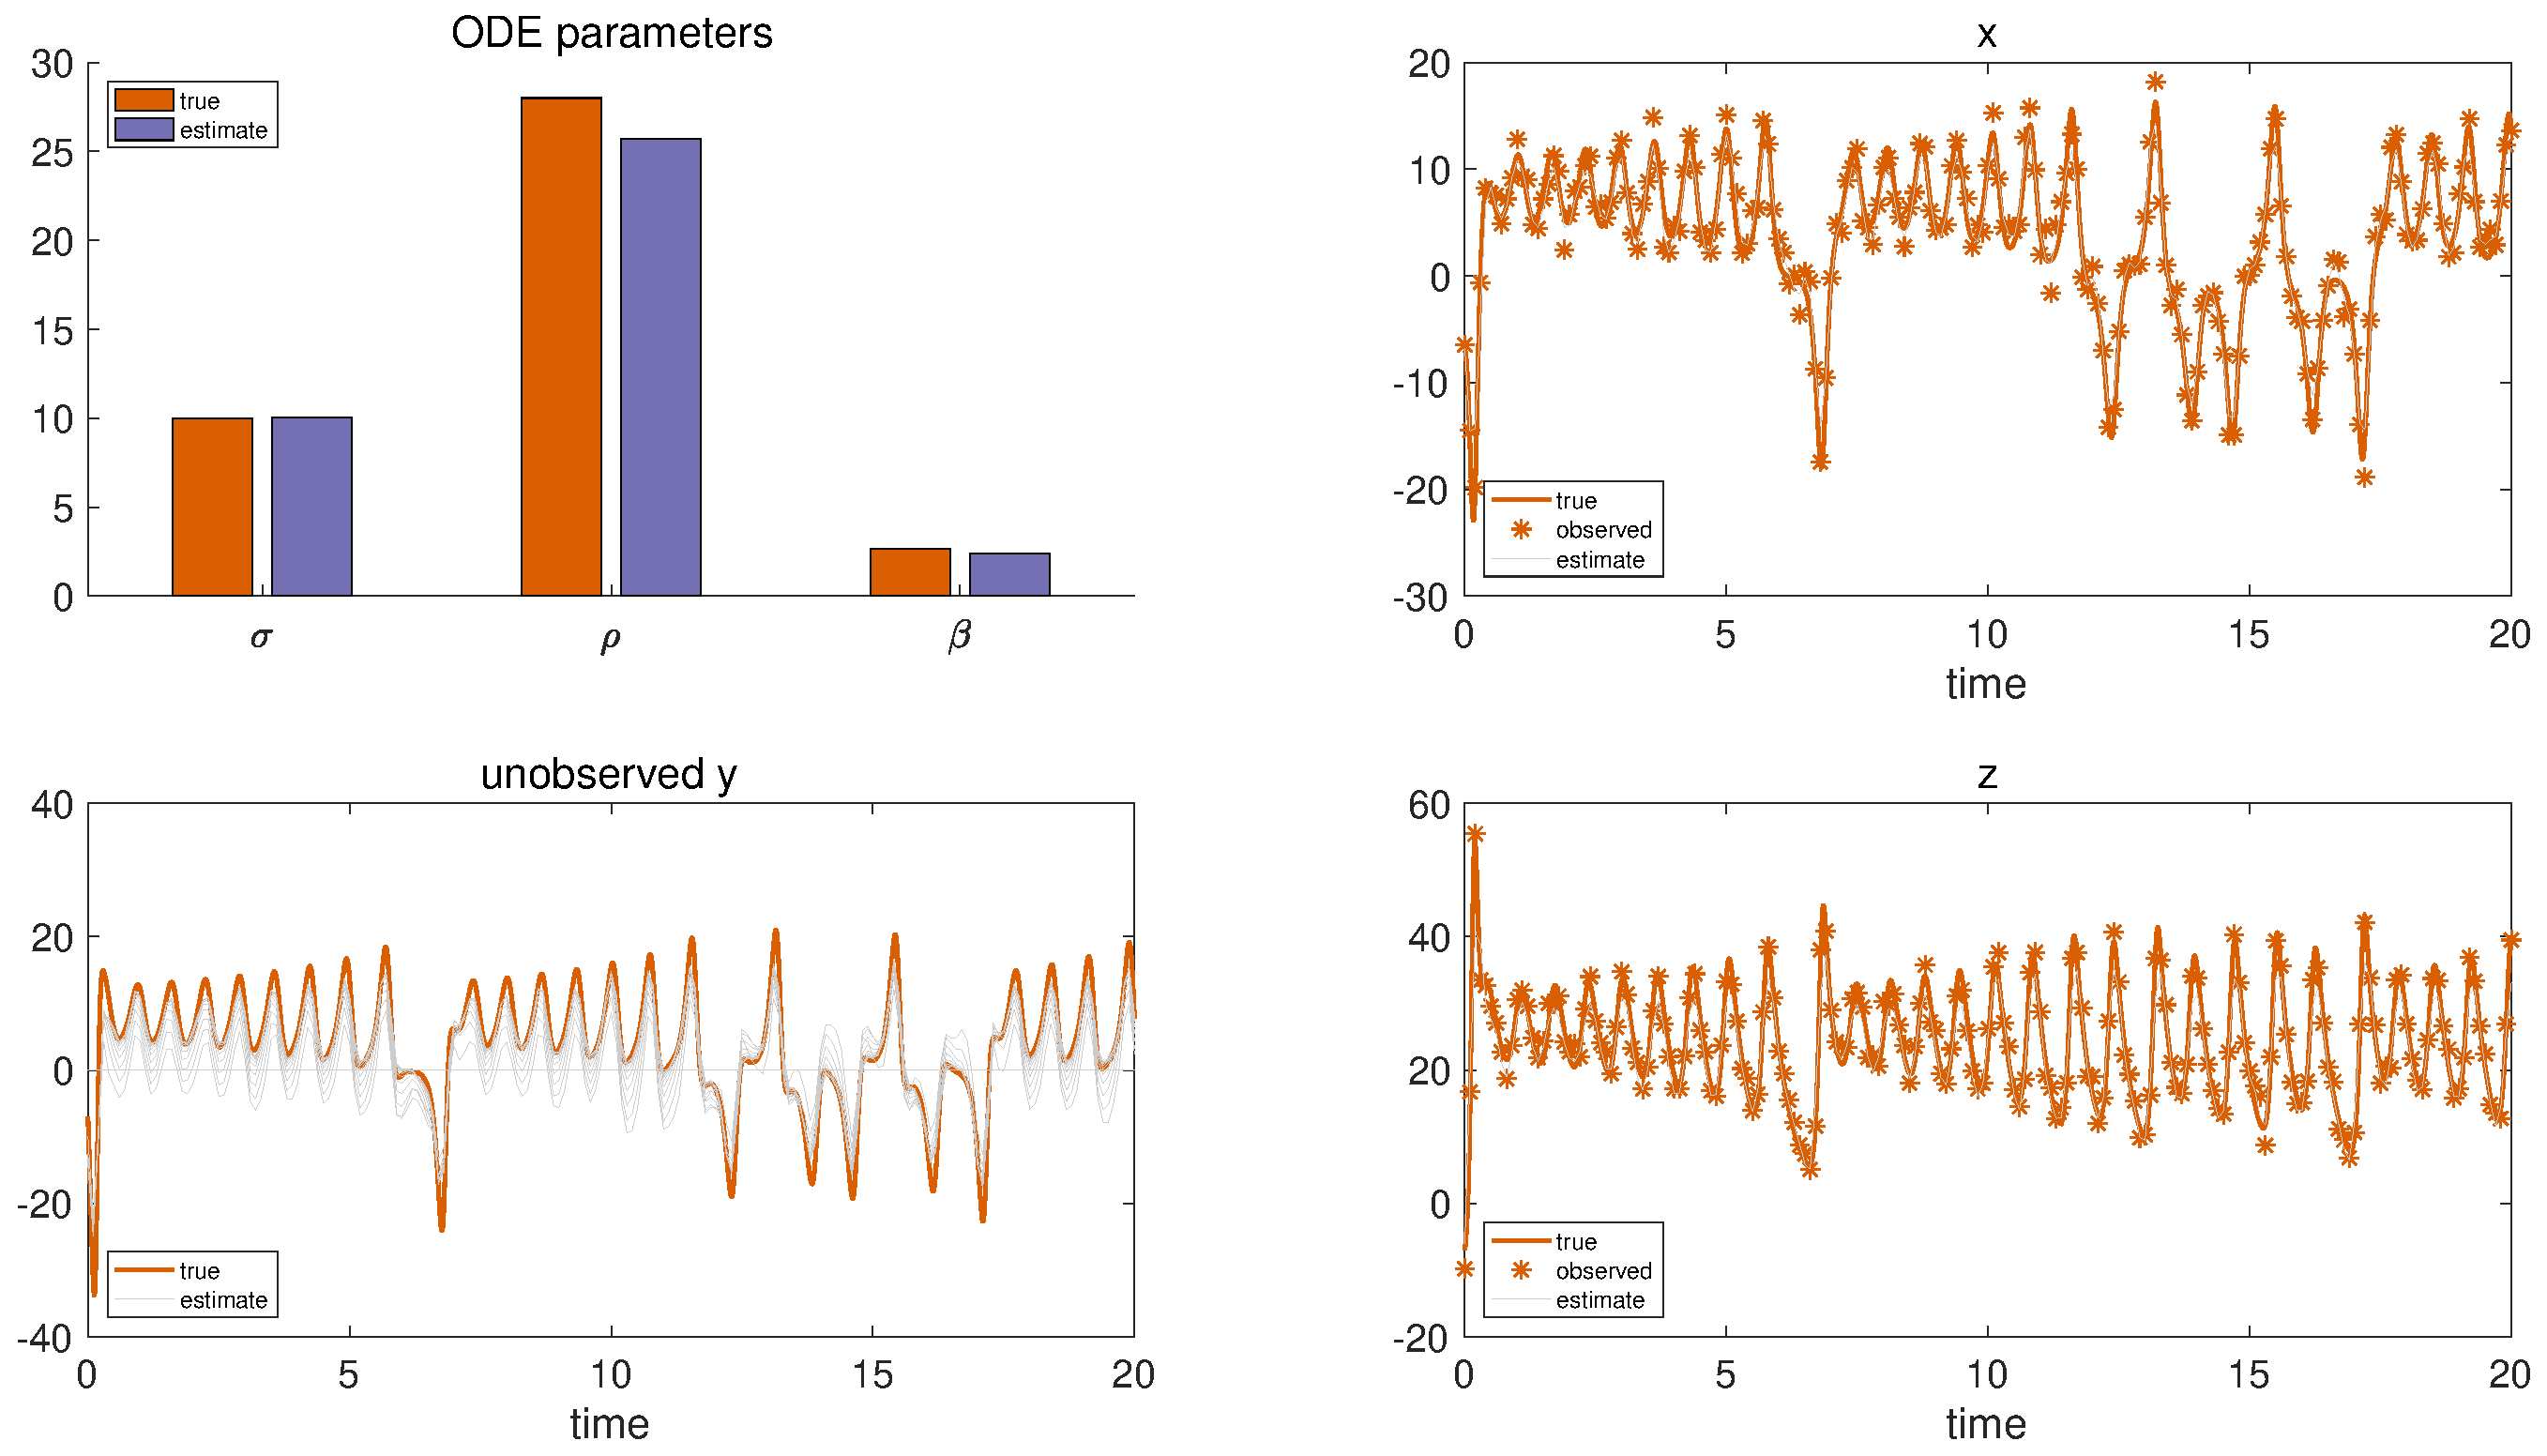
\includegraphics [width=4in]{Lorenz_attractor_4_20.eps}

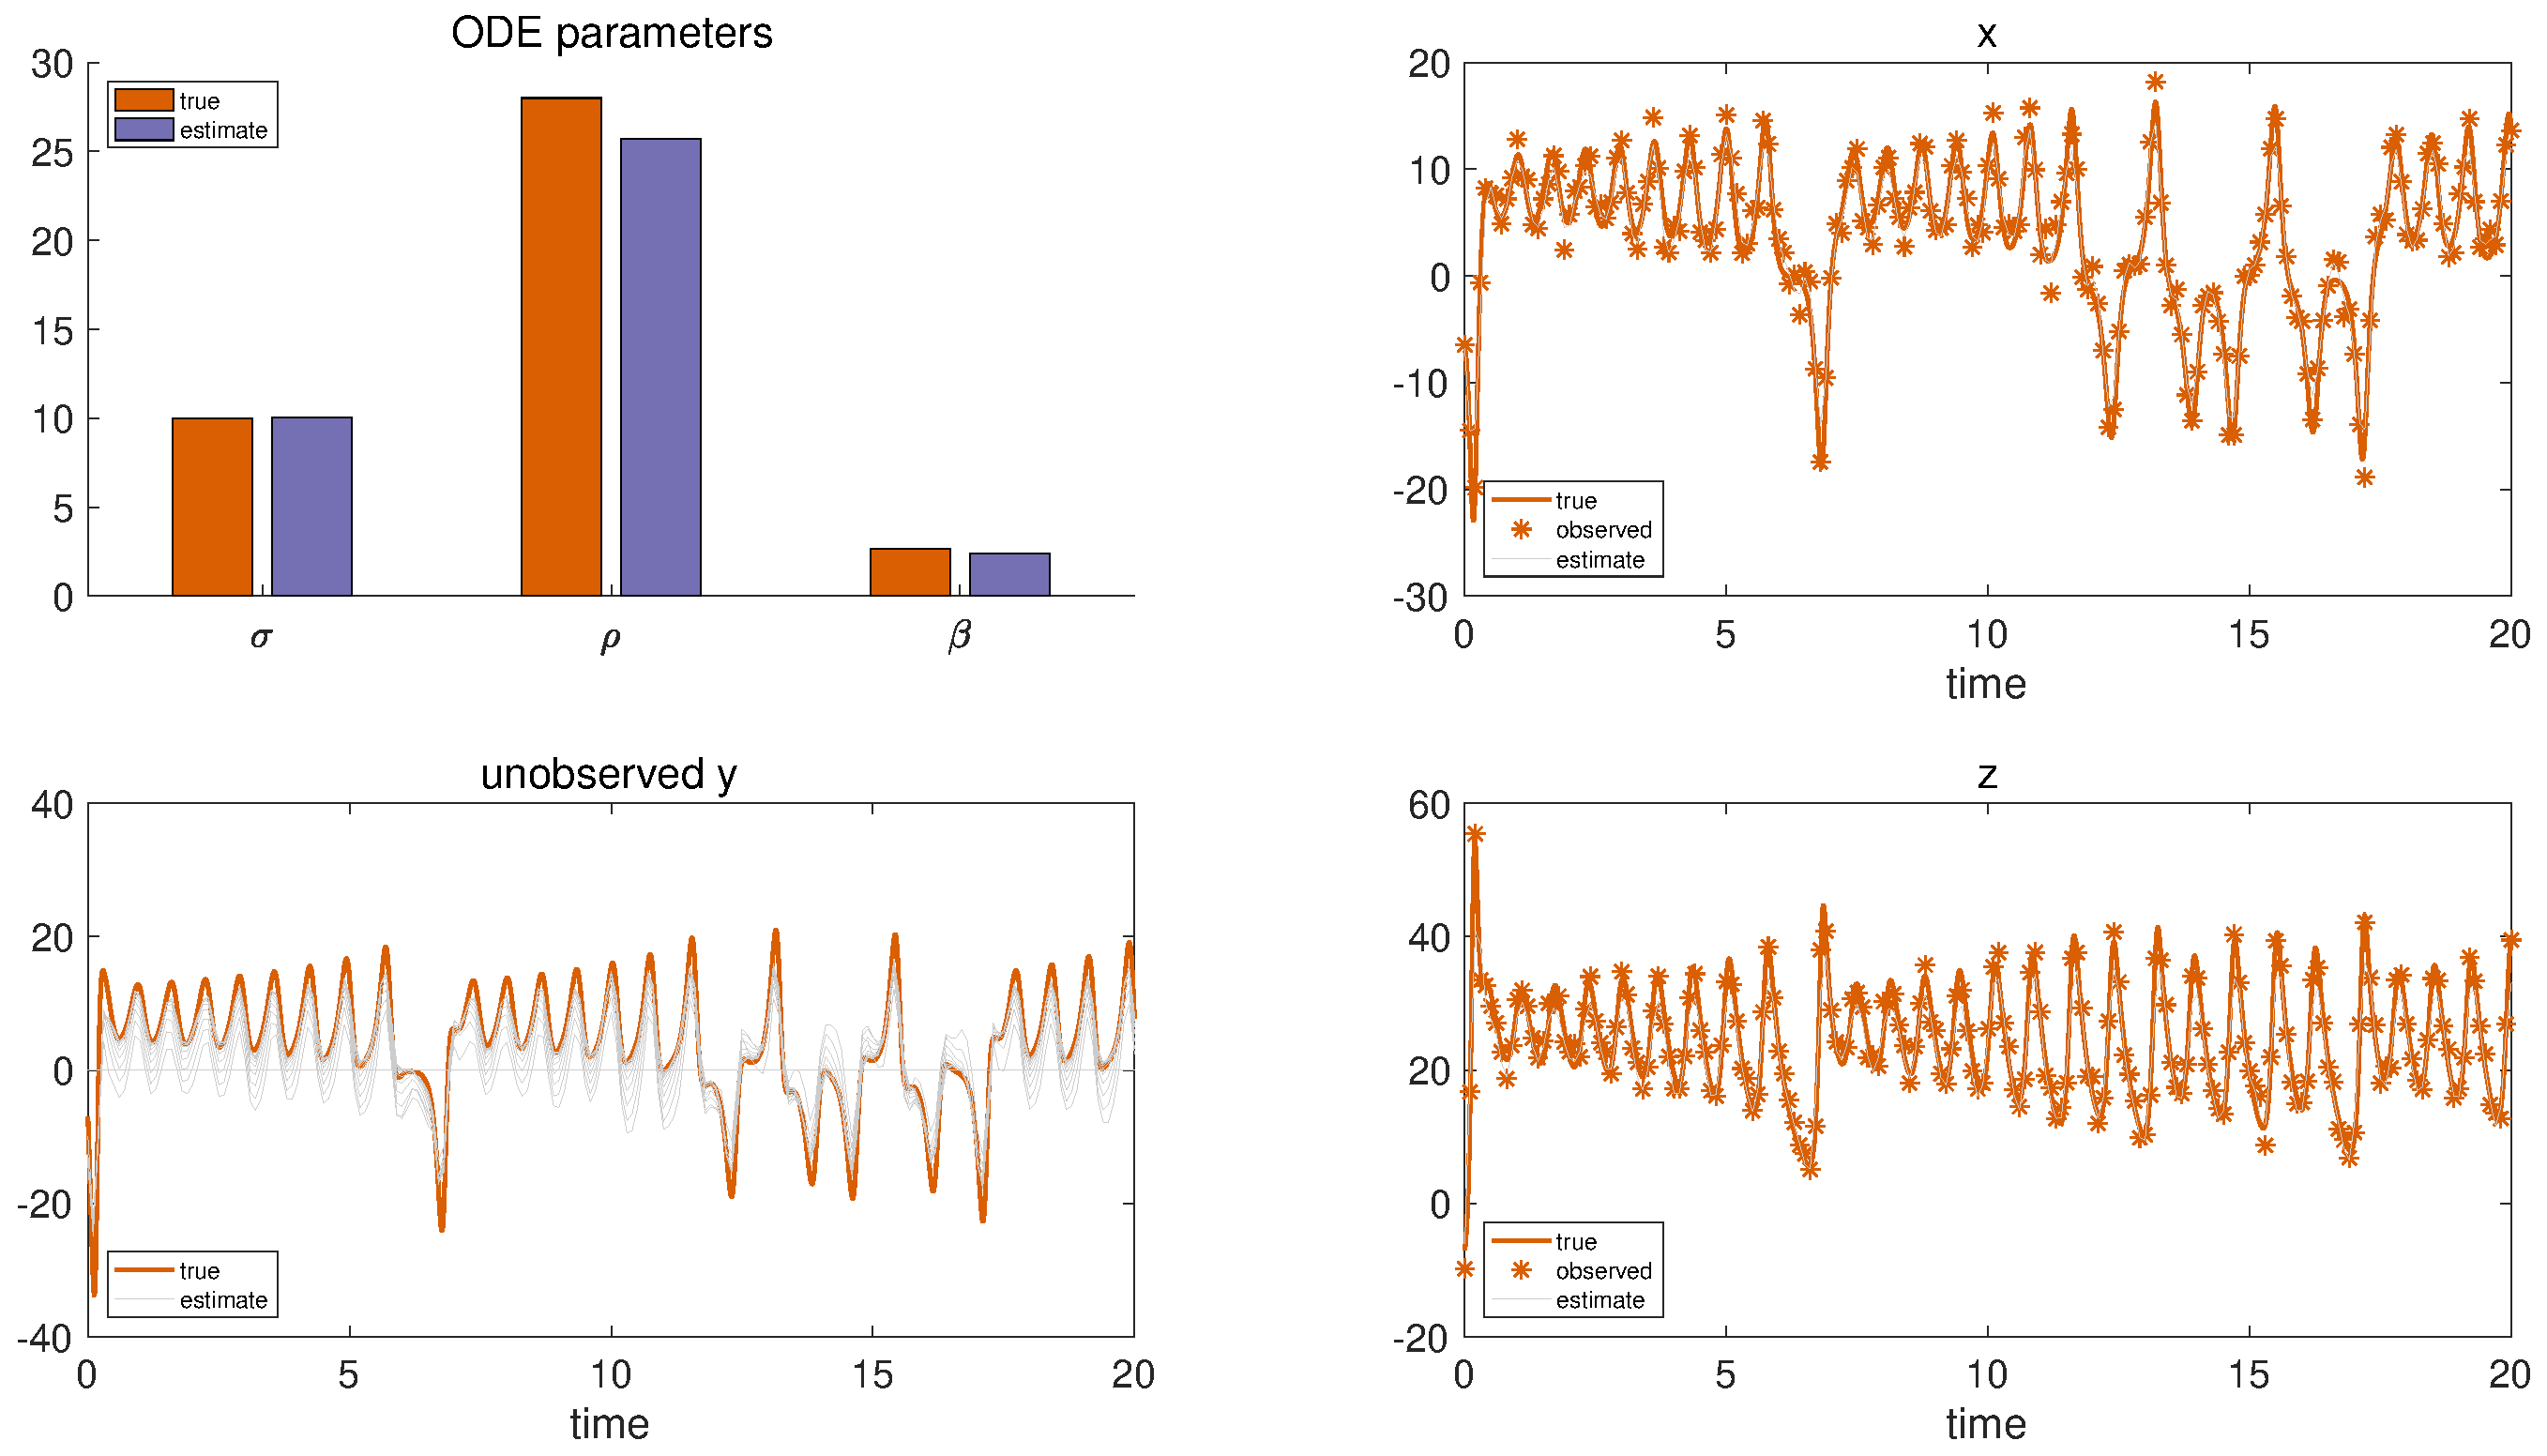
\includegraphics [width=4in]{Lorenz_attractor_4_21.eps}

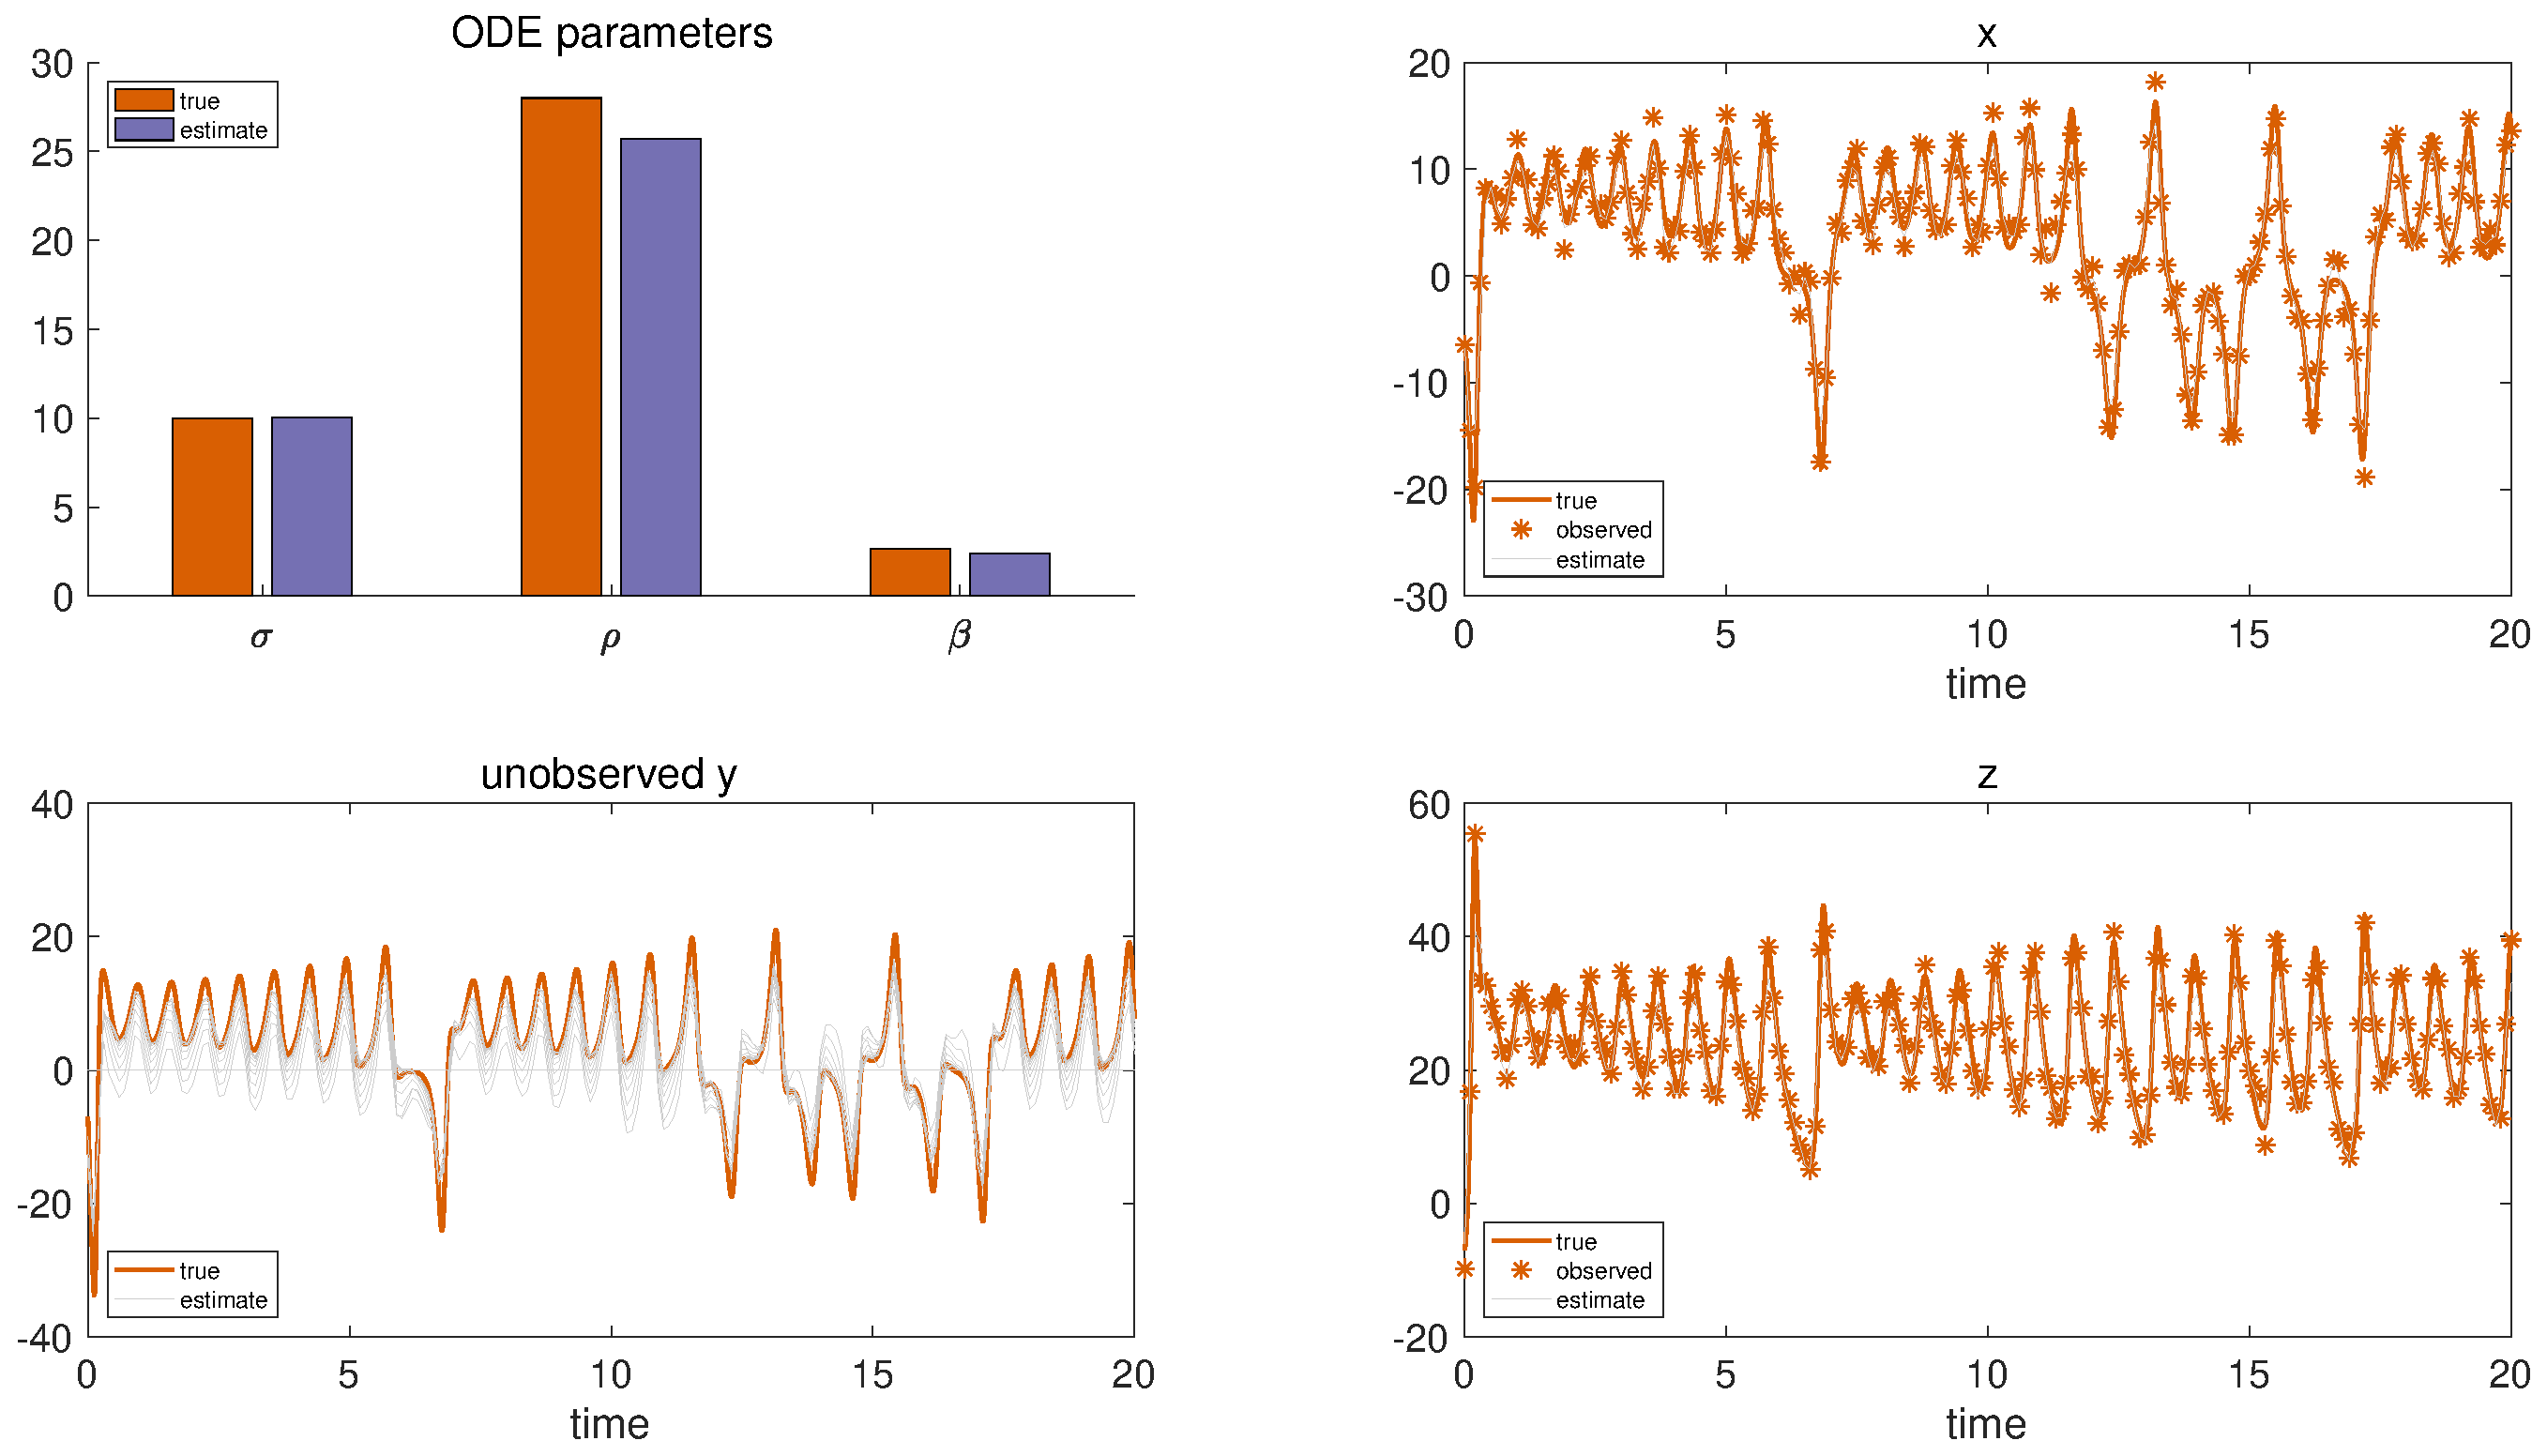
\includegraphics [width=4in]{Lorenz_attractor_4_22.eps}

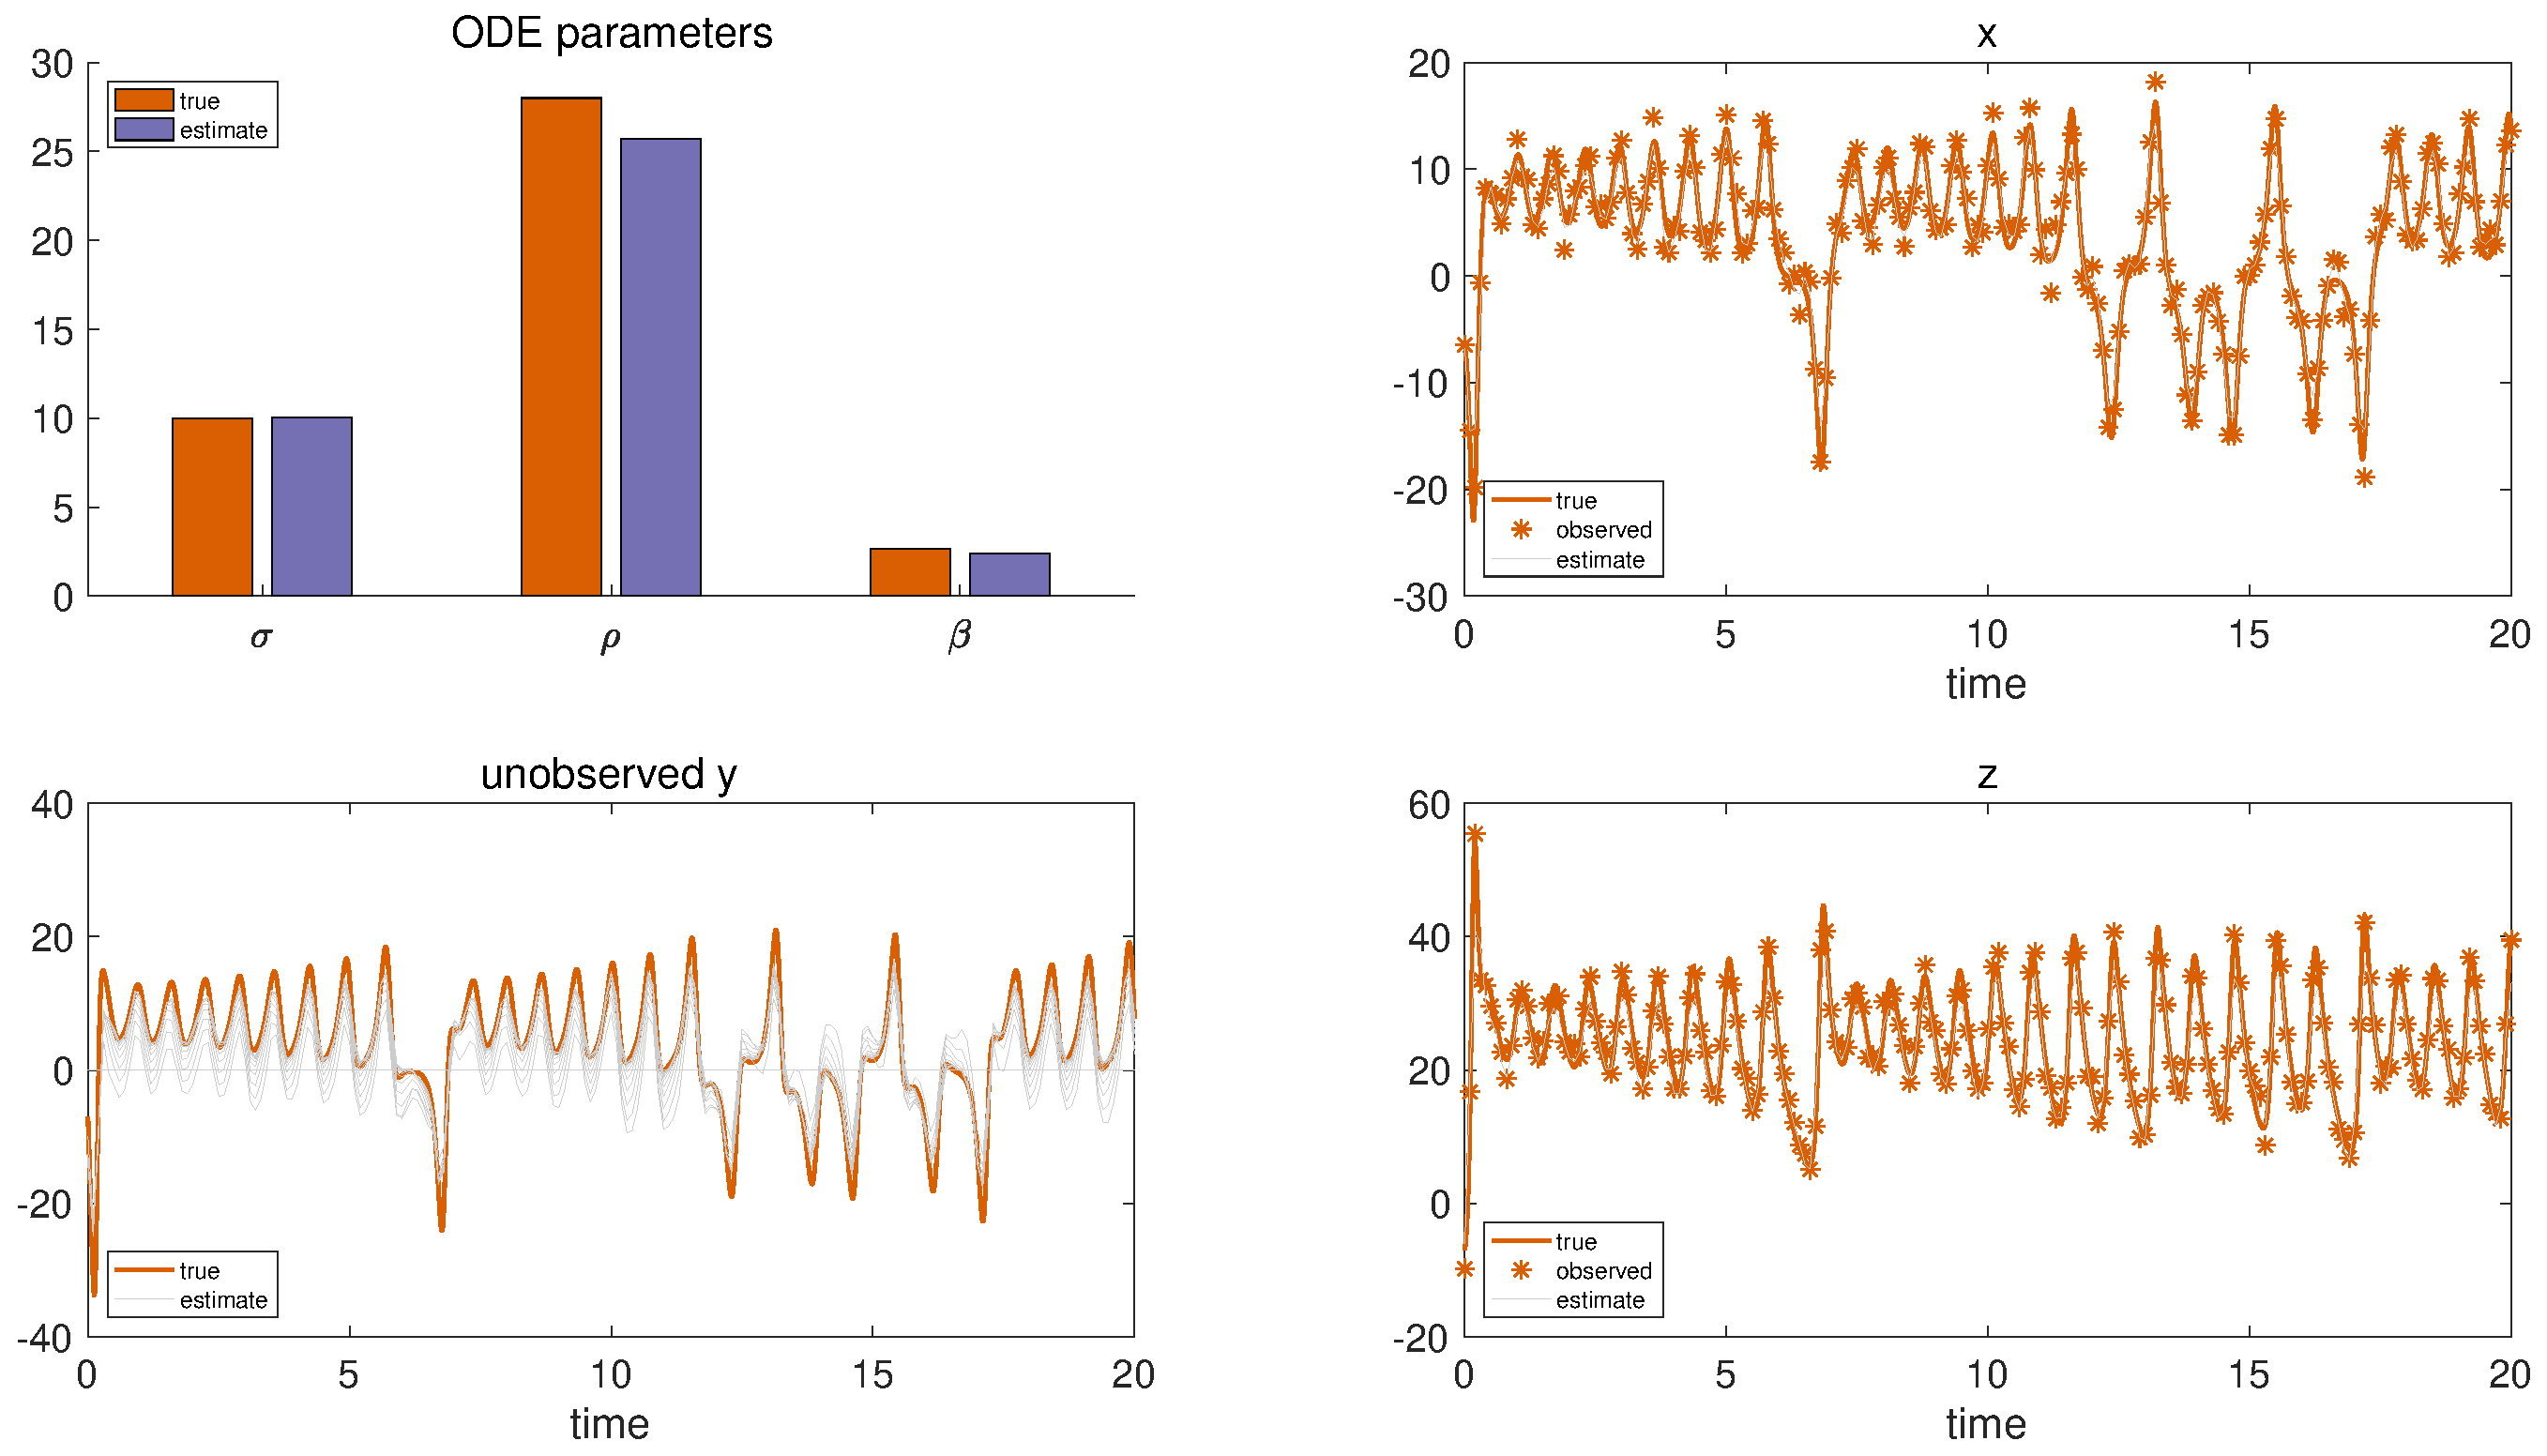
\includegraphics [width=4in]{Lorenz_attractor_4_23.eps}

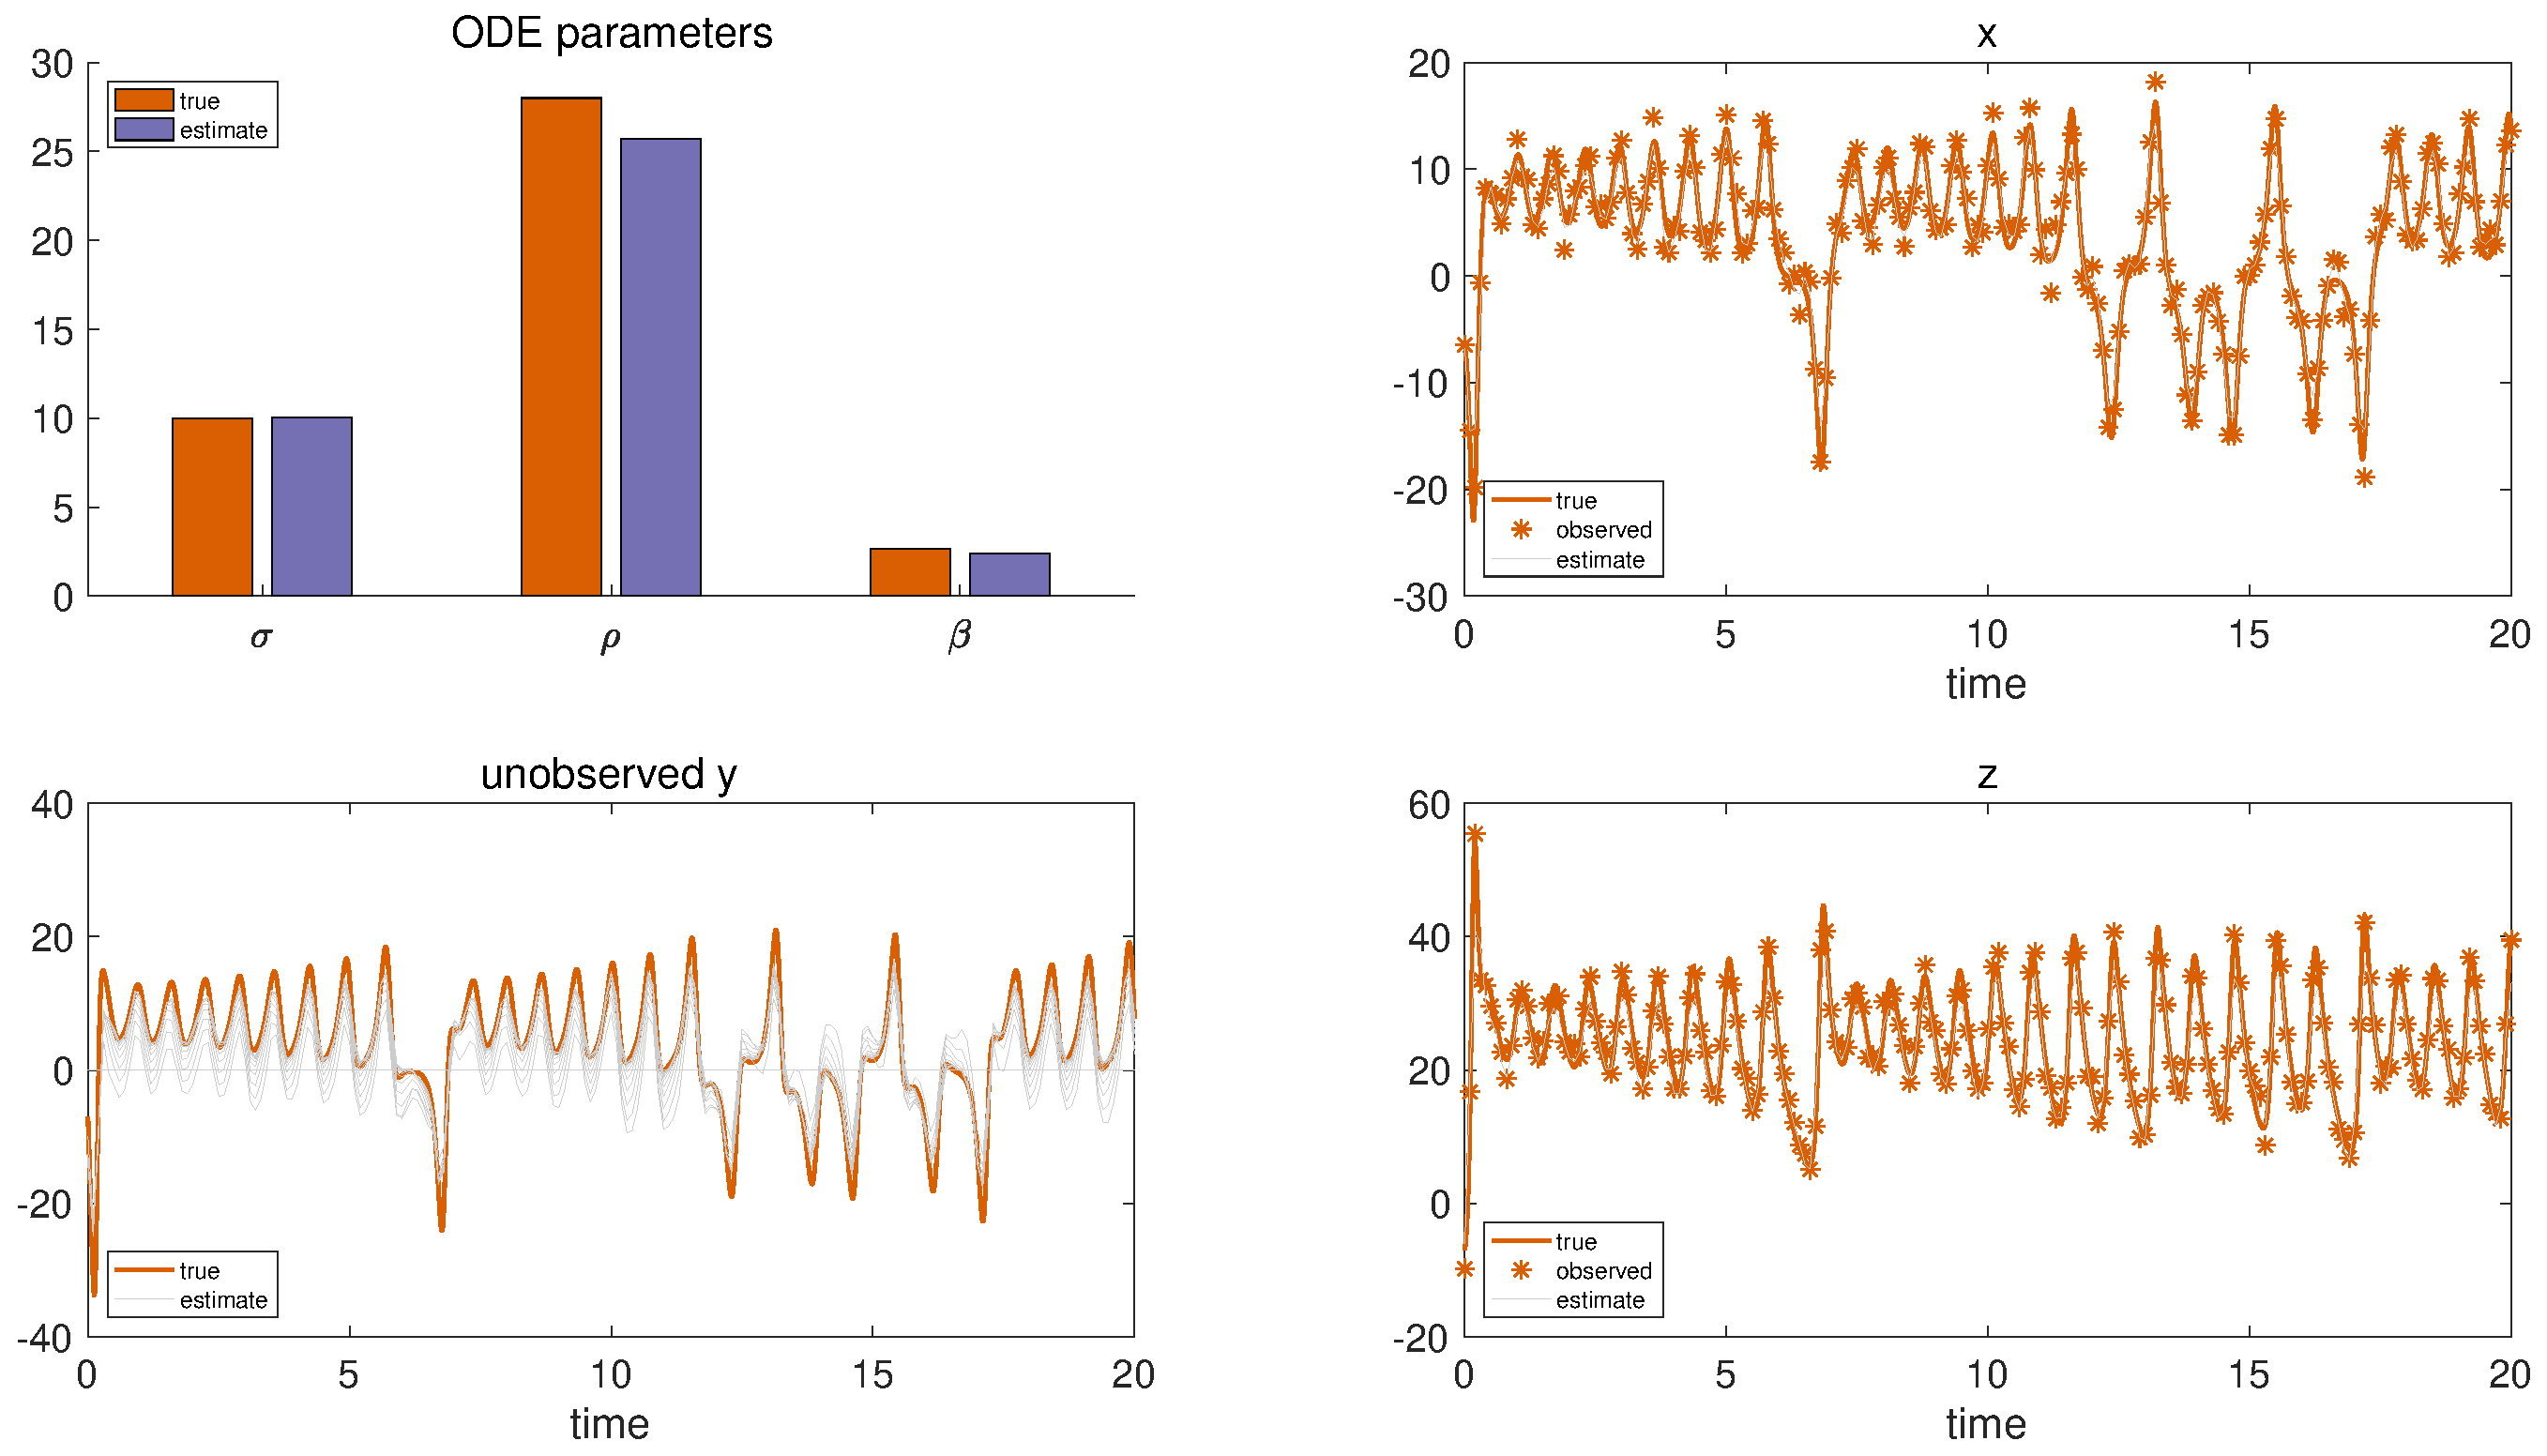
\includegraphics [width=4in]{Lorenz_attractor_4_24.eps}

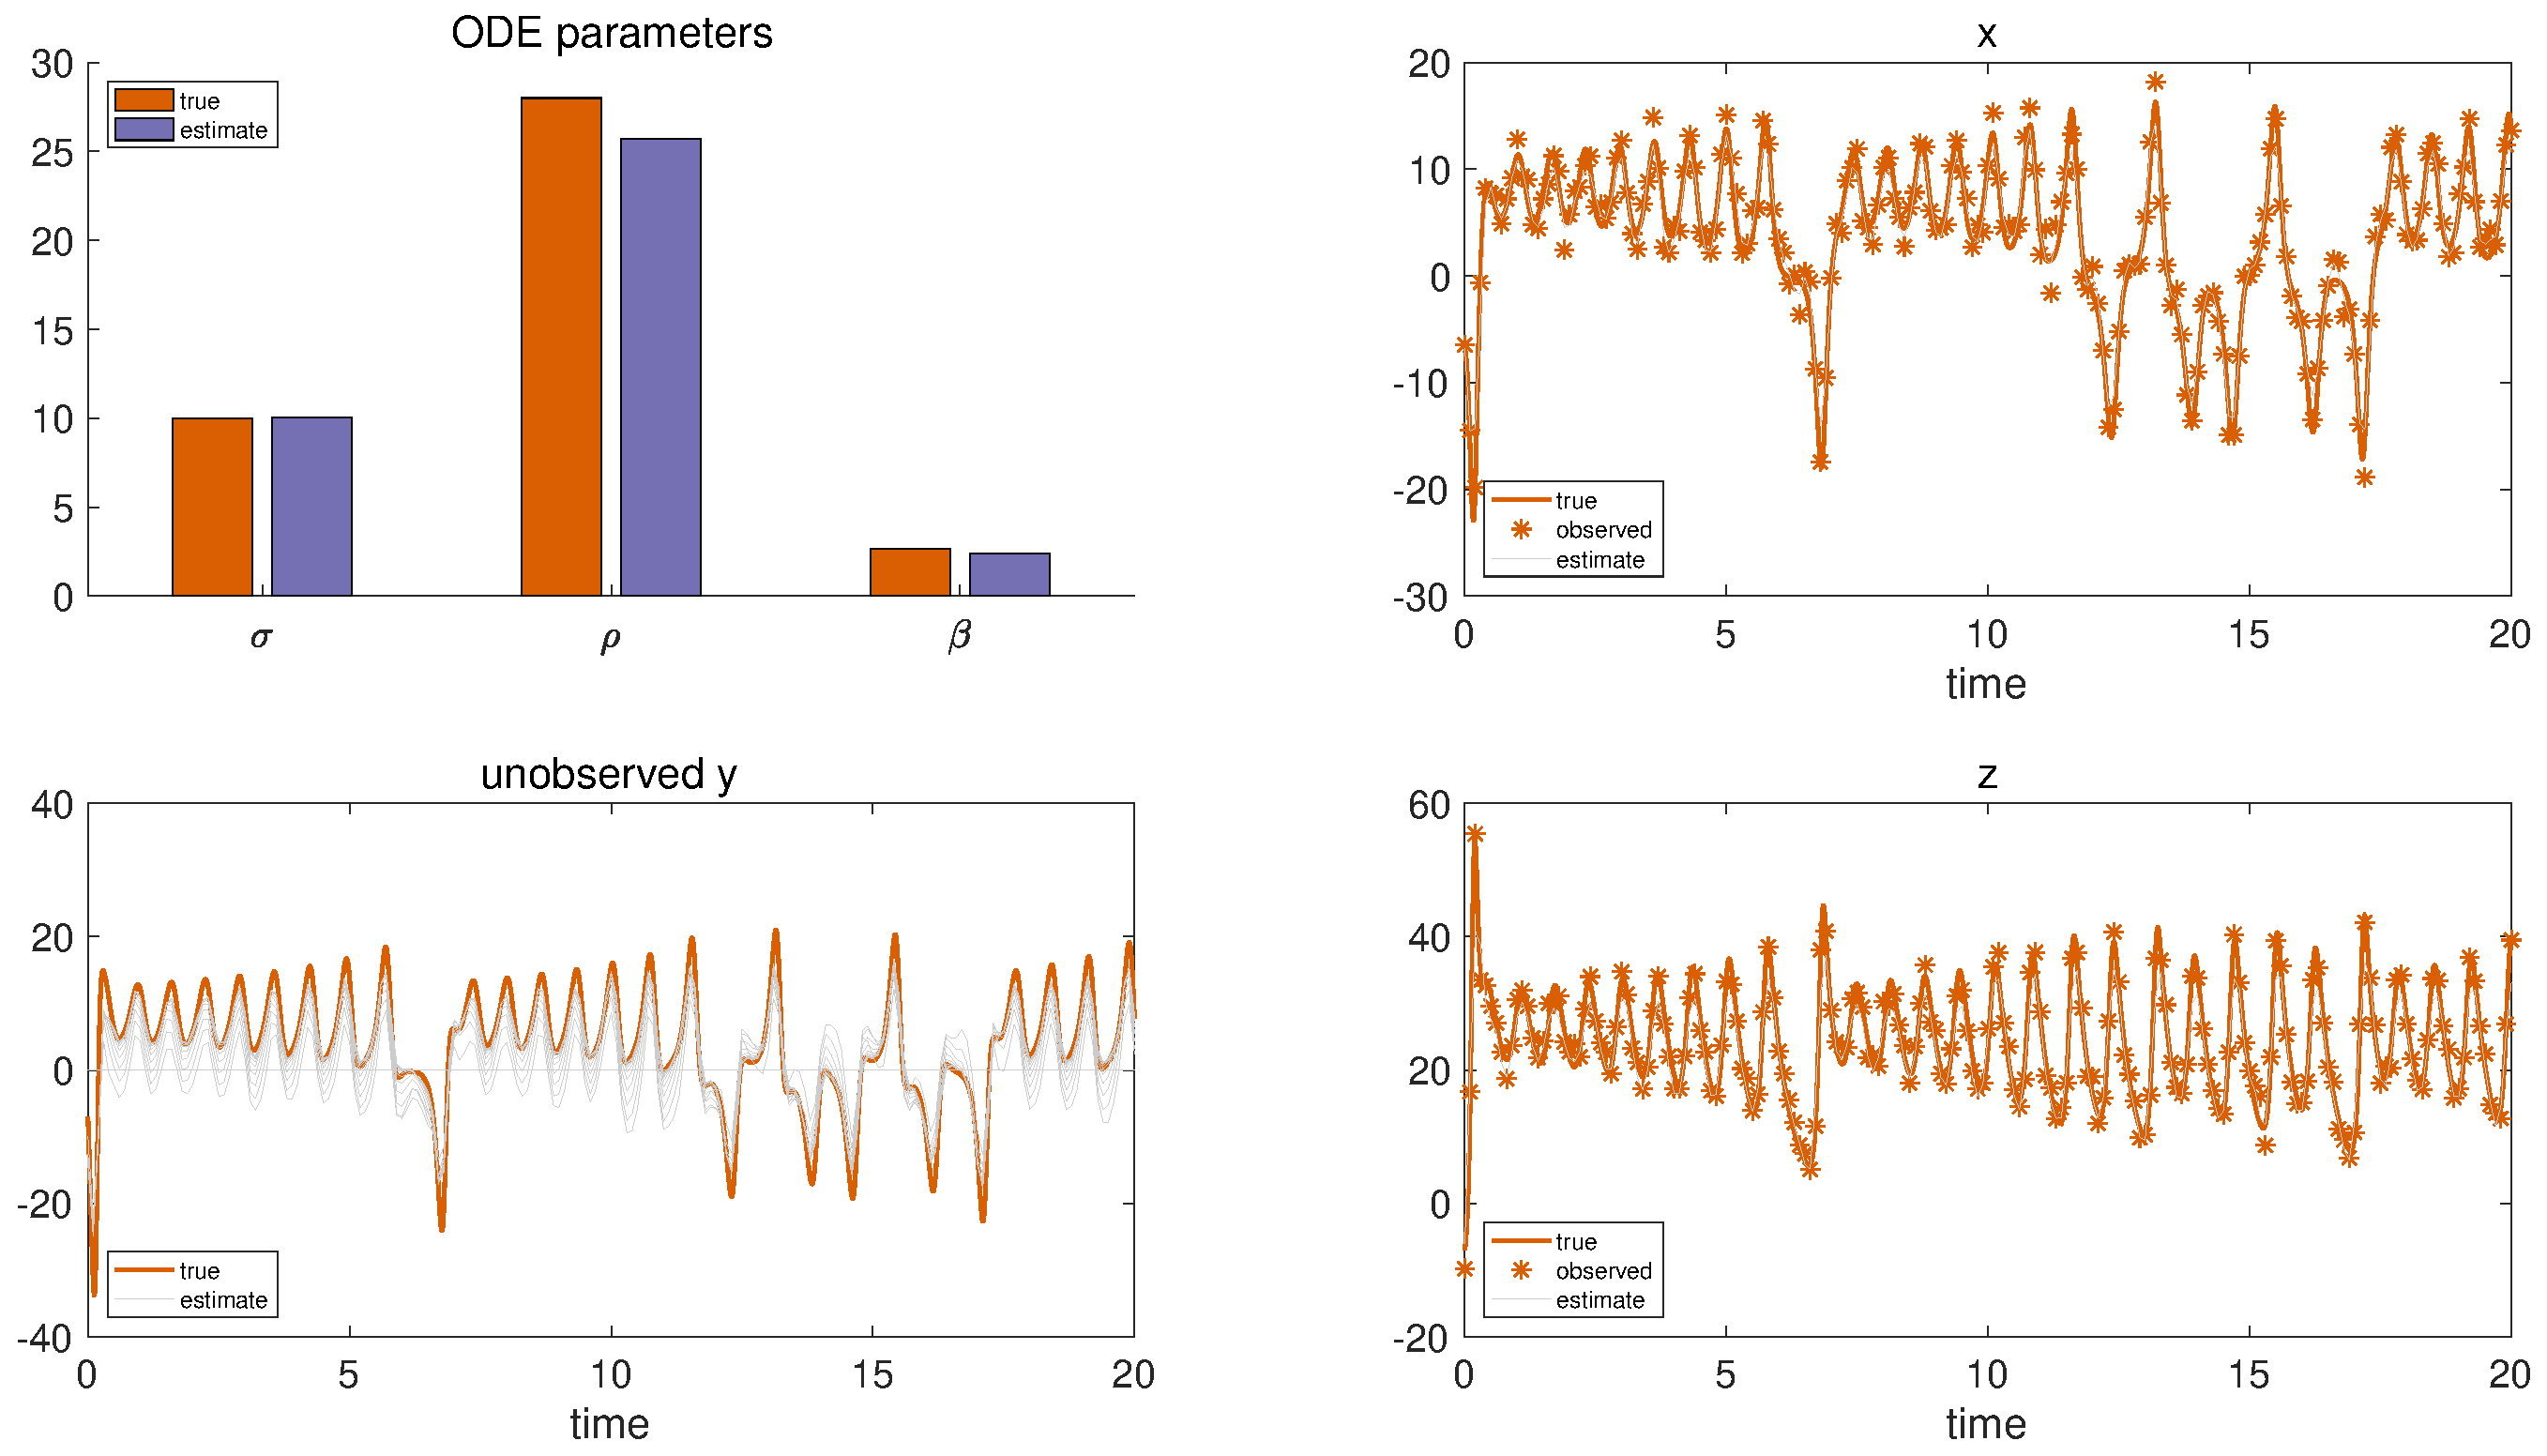
\includegraphics [width=4in]{Lorenz_attractor_4_25.eps}

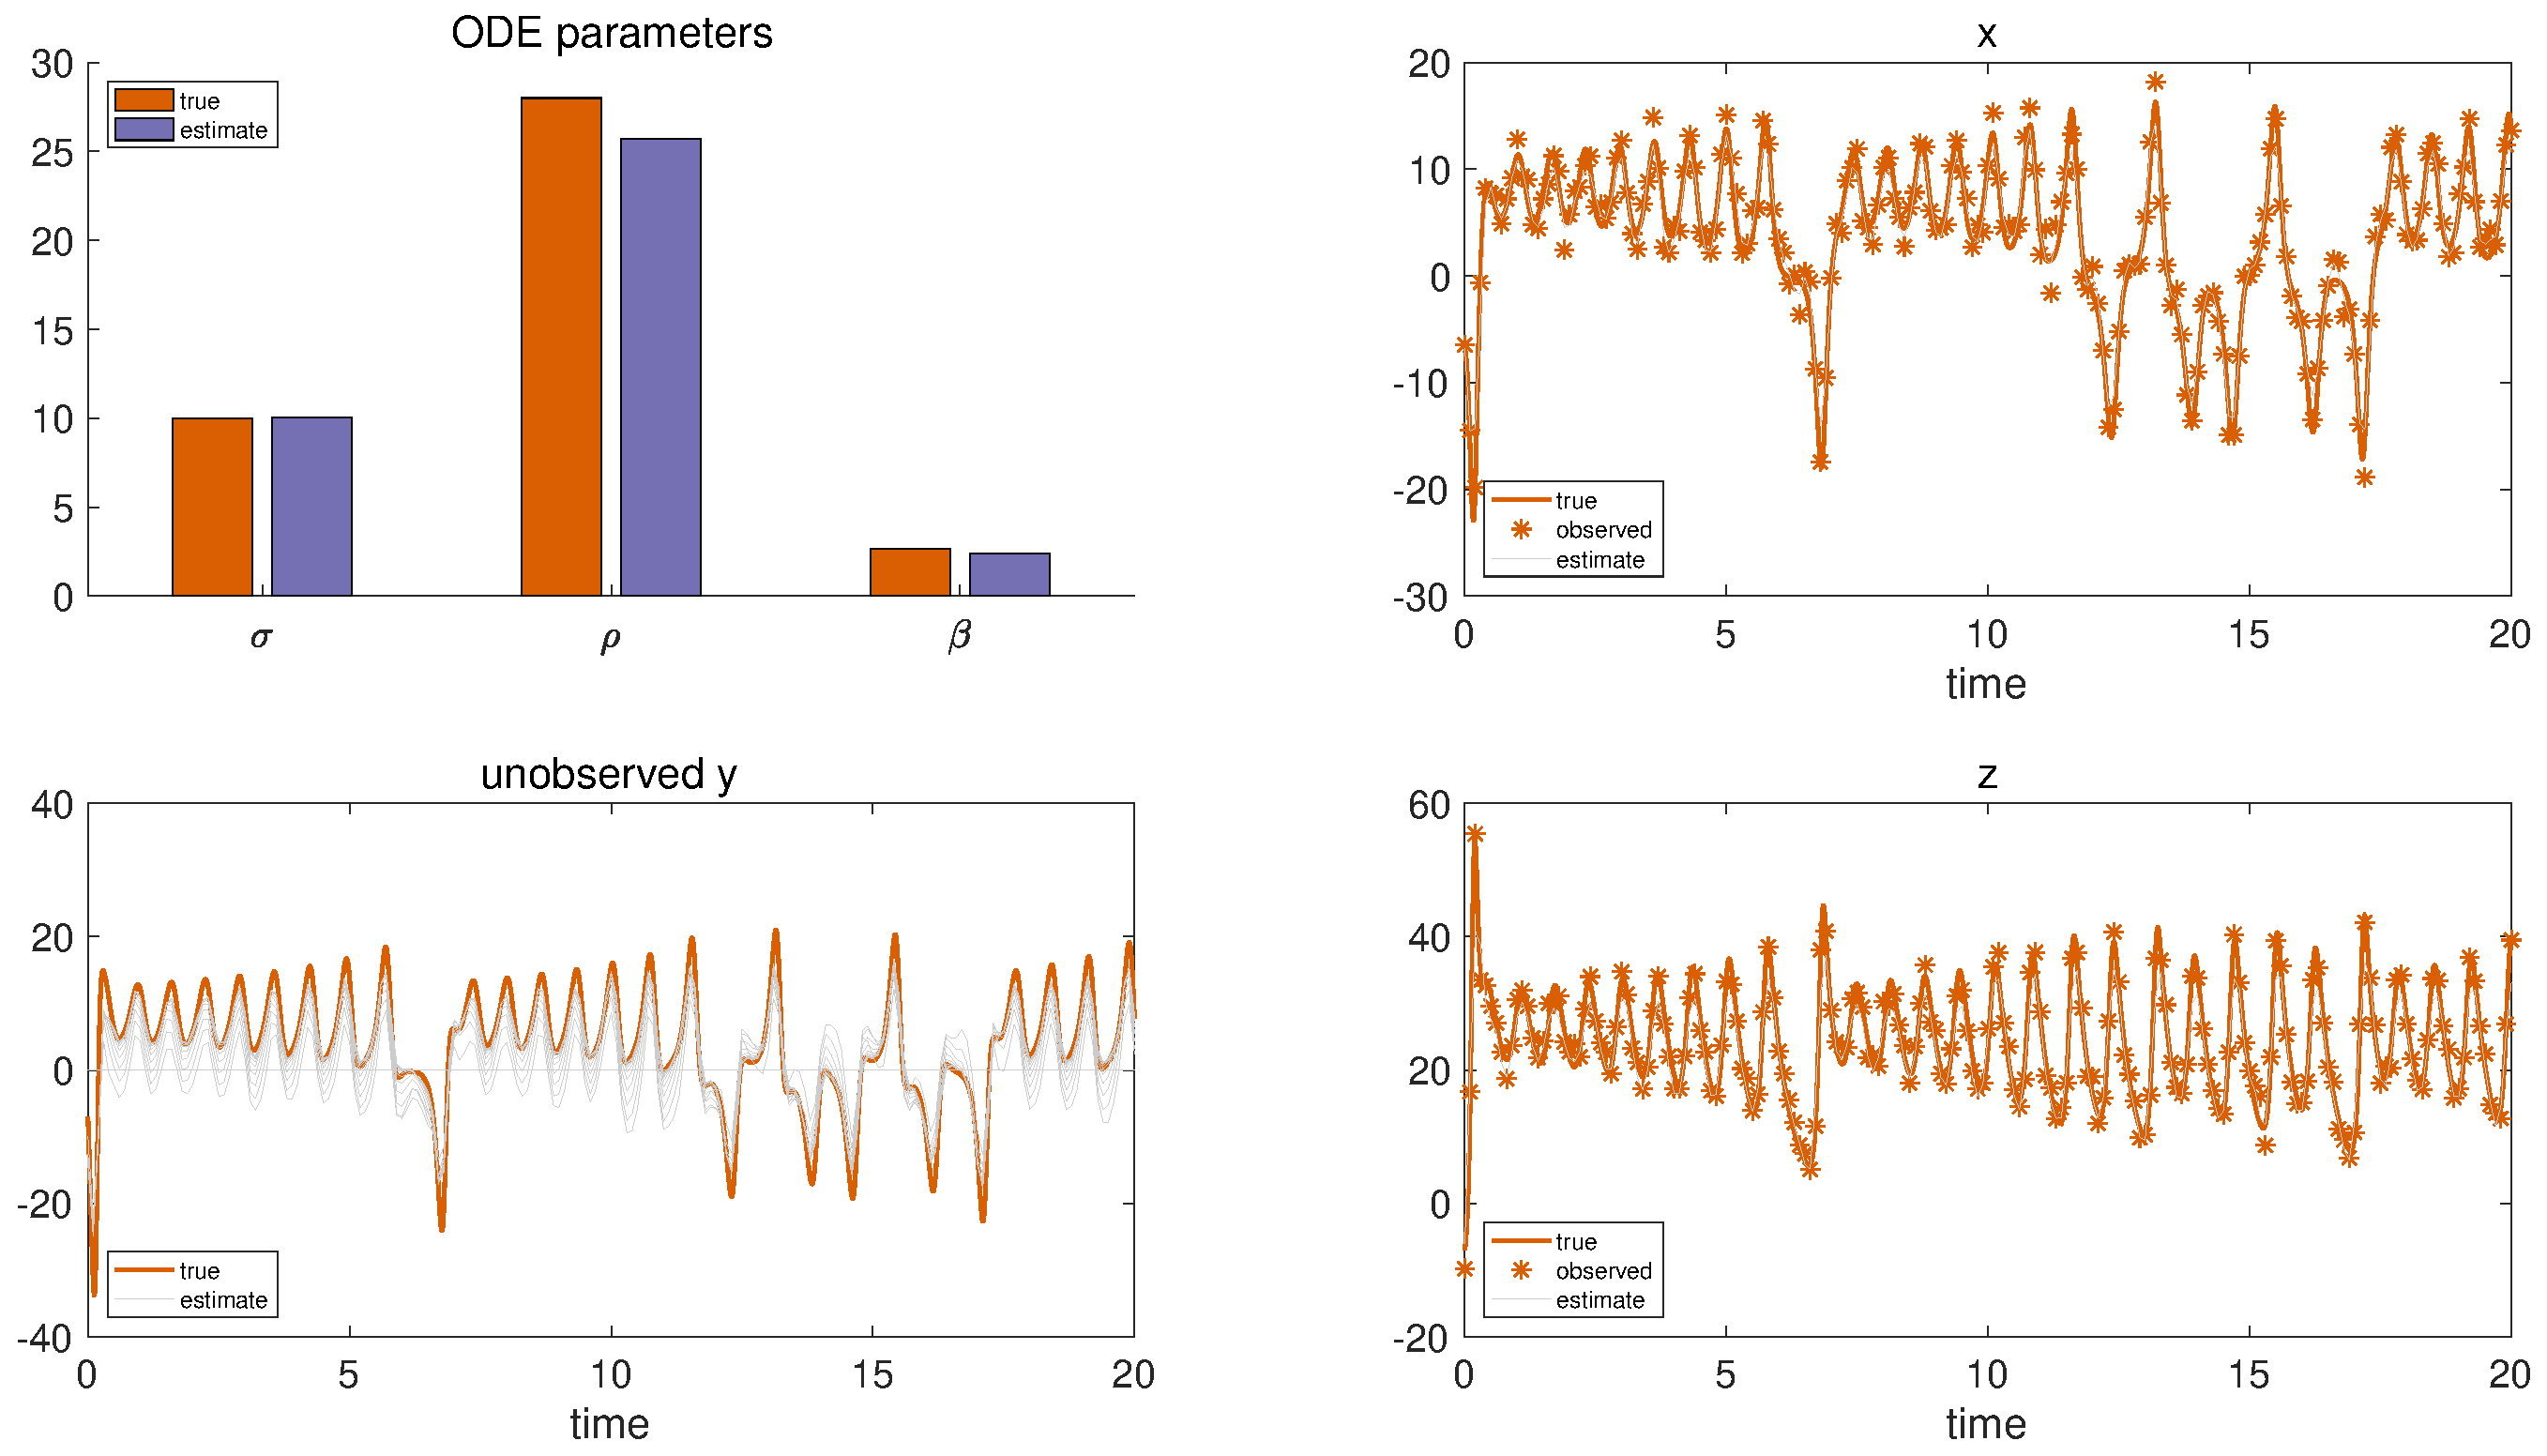
\includegraphics [width=4in]{Lorenz_attractor_4_26.eps}

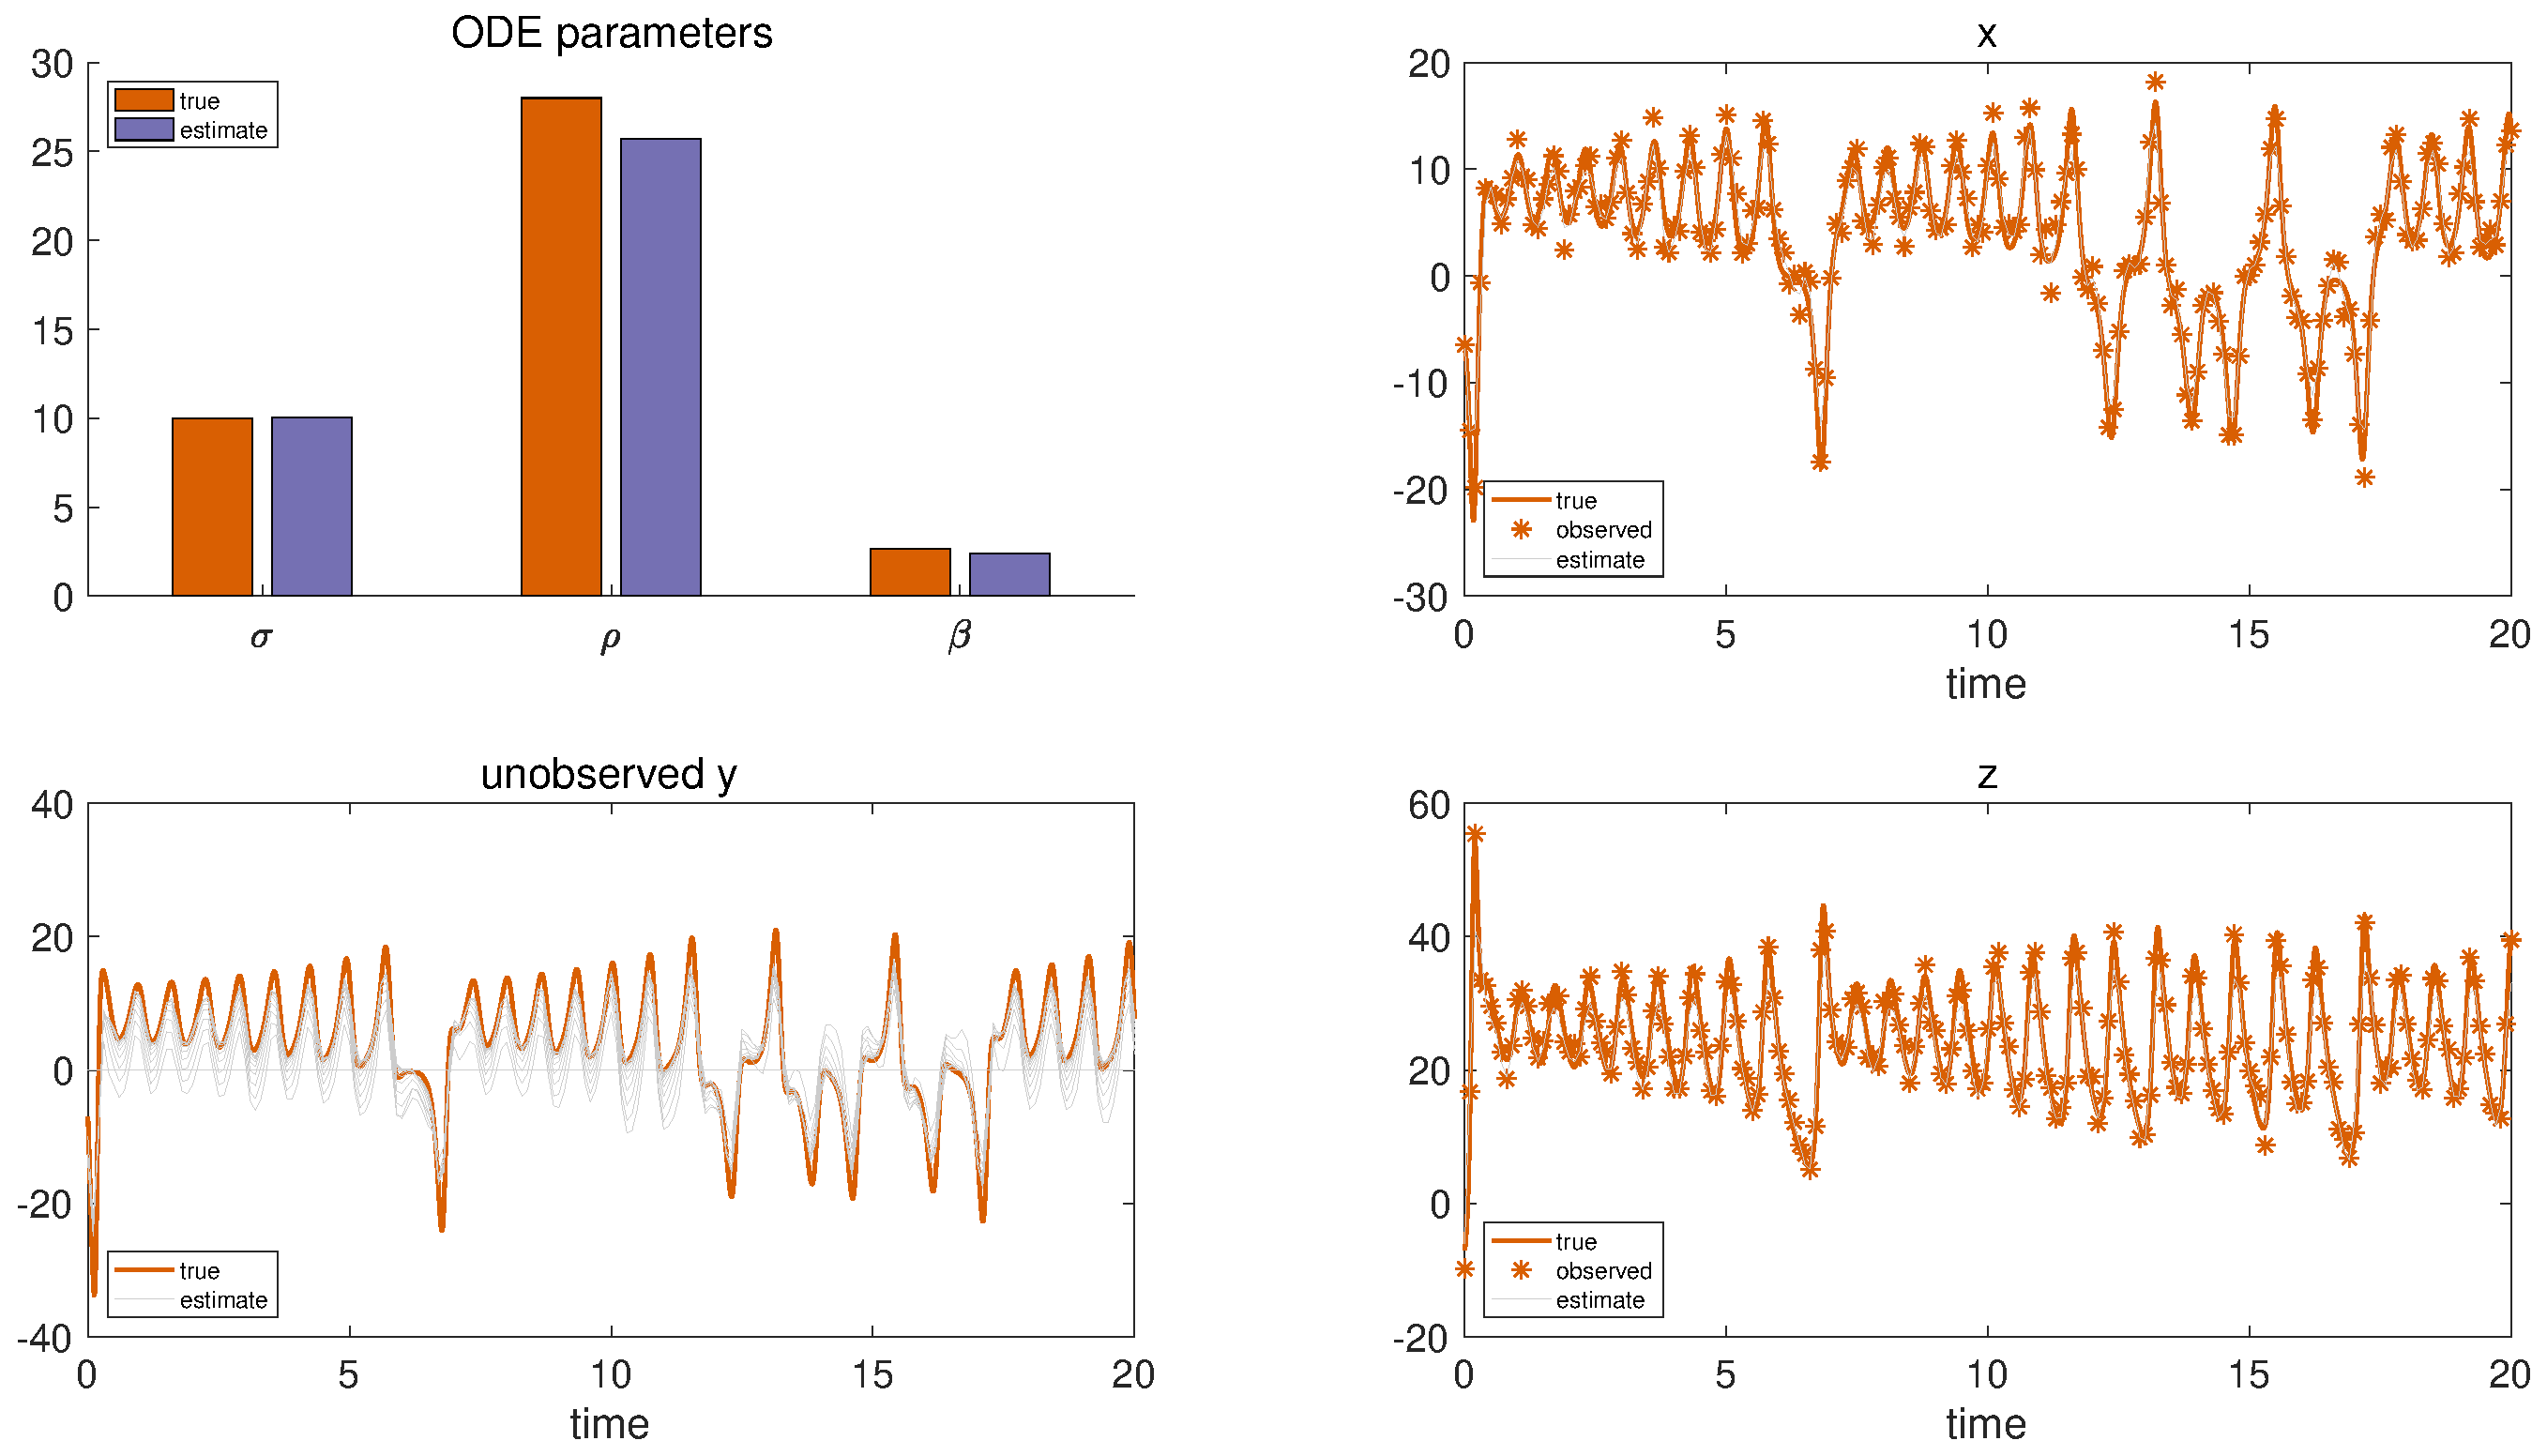
\includegraphics [width=4in]{Lorenz_attractor_4_27.eps}

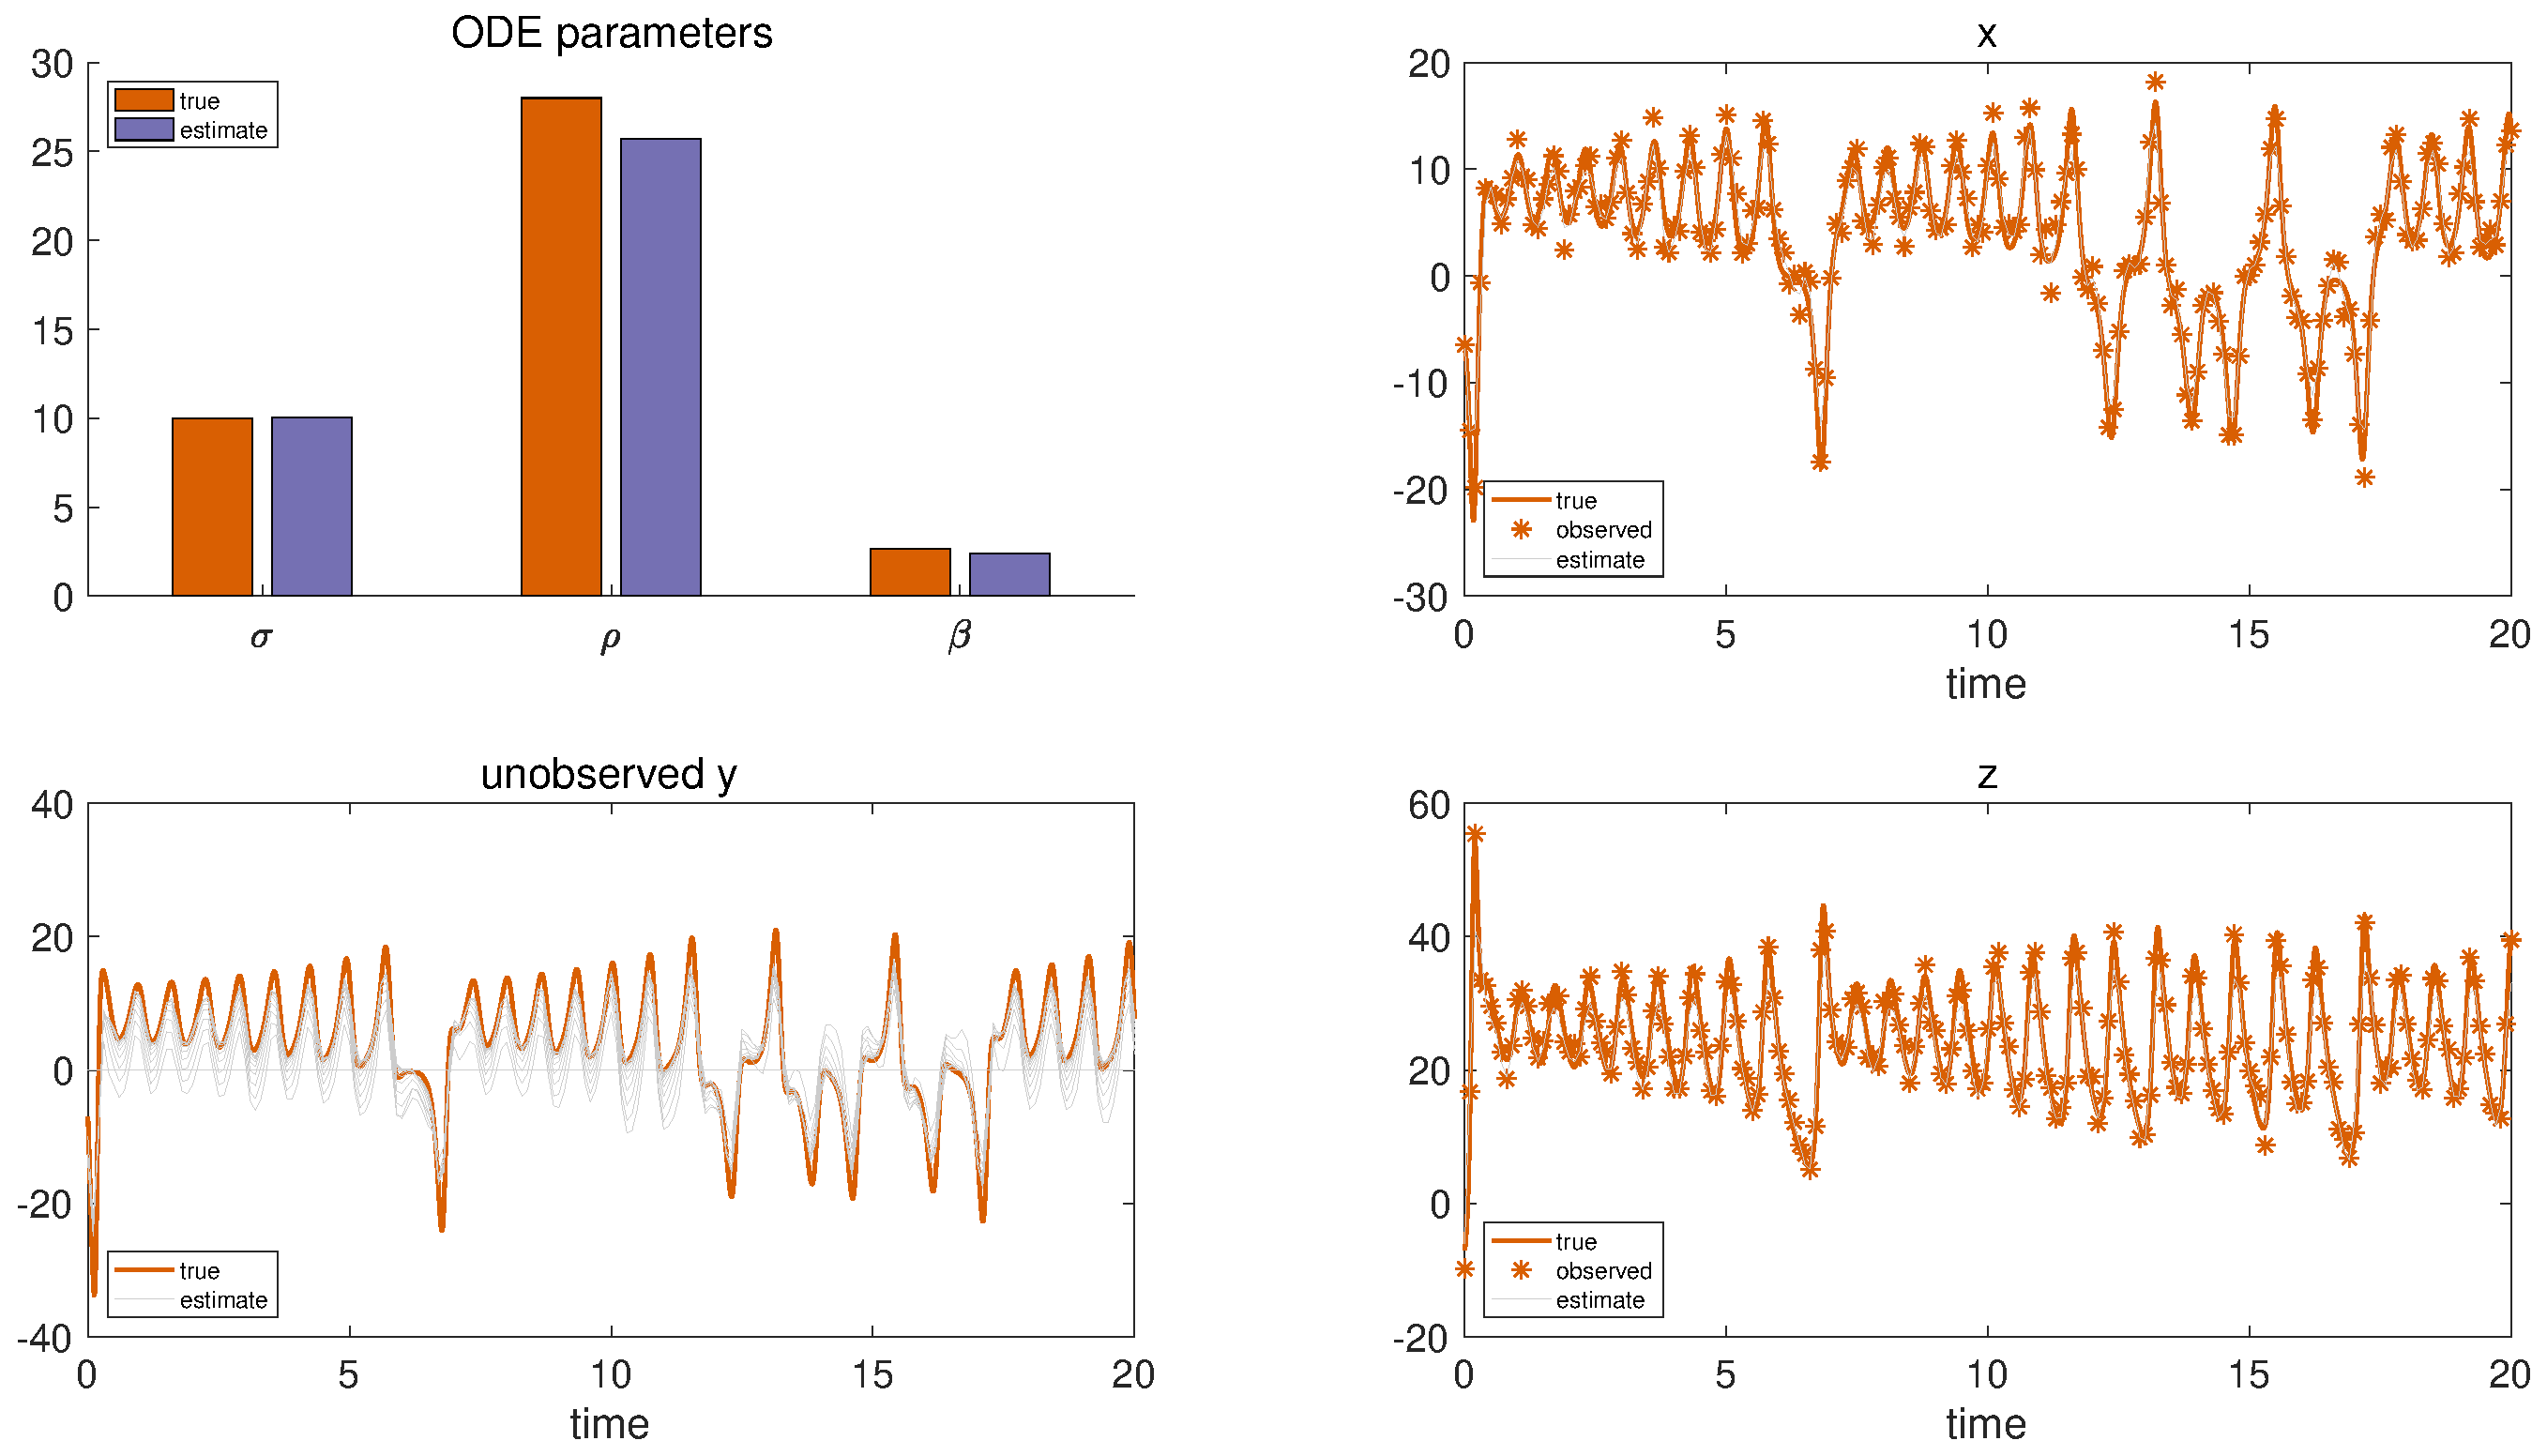
\includegraphics [width=4in]{Lorenz_attractor_4_28.eps}

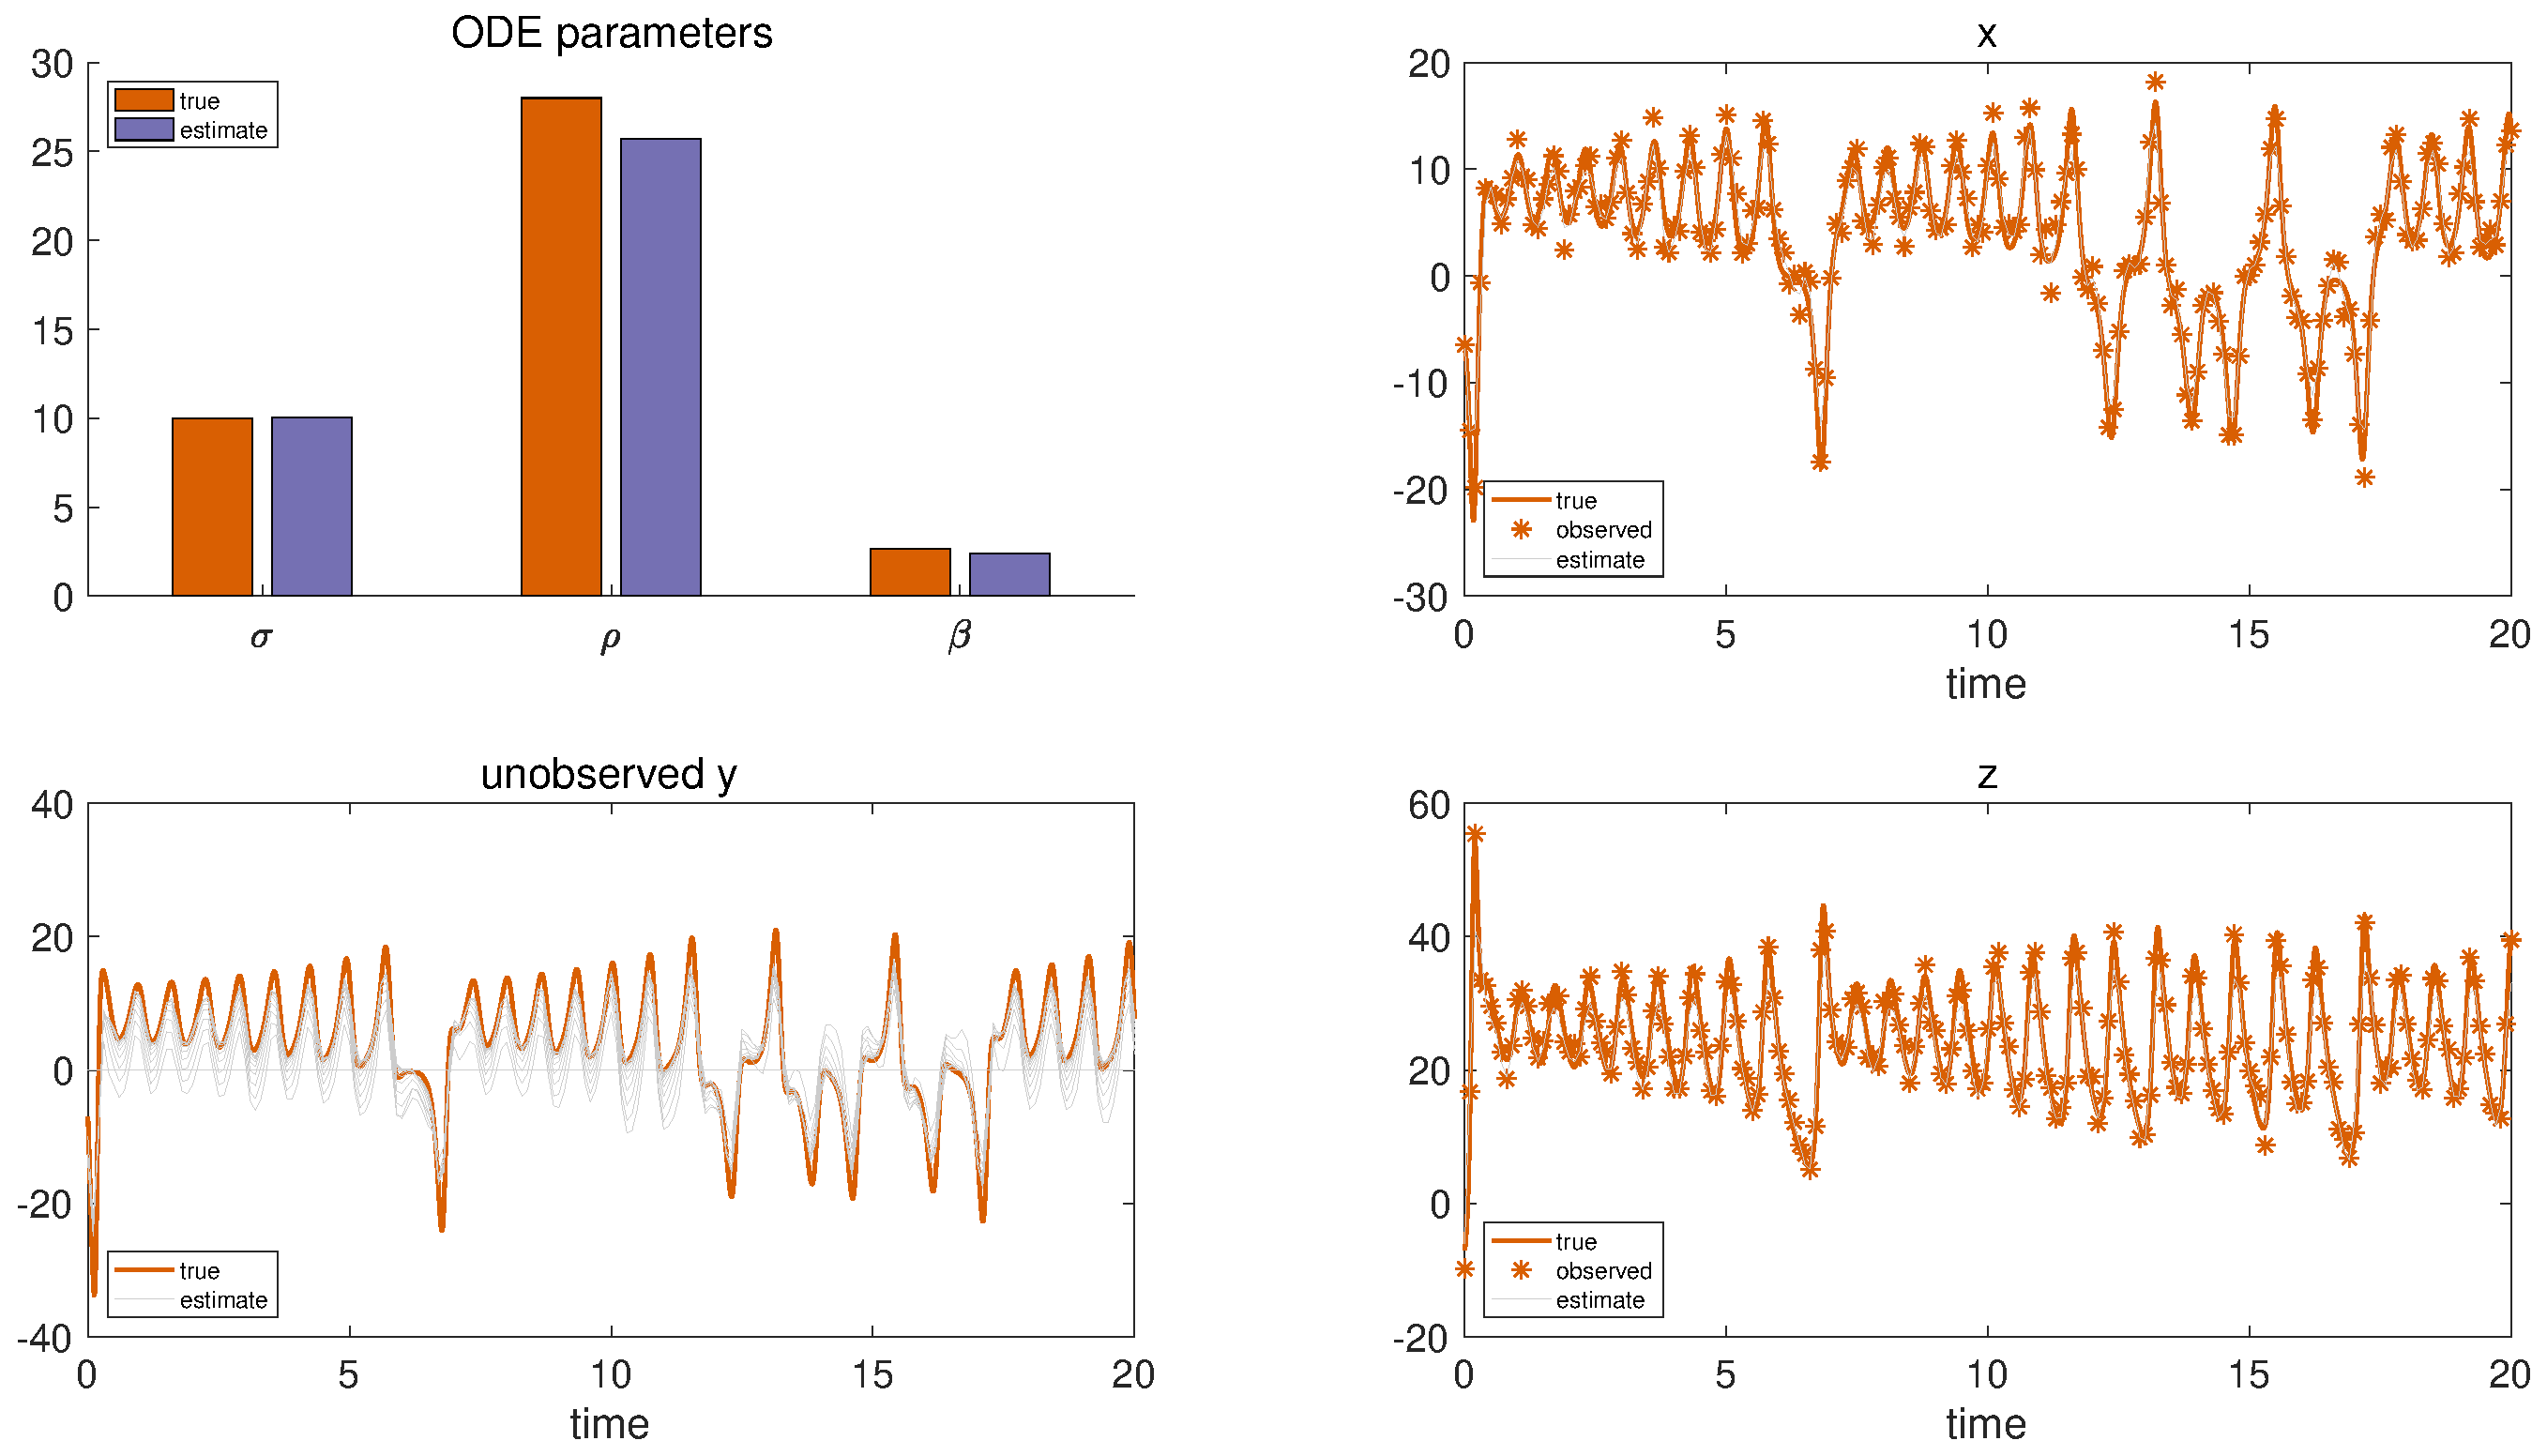
\includegraphics [width=4in]{Lorenz_attractor_4_29.eps}

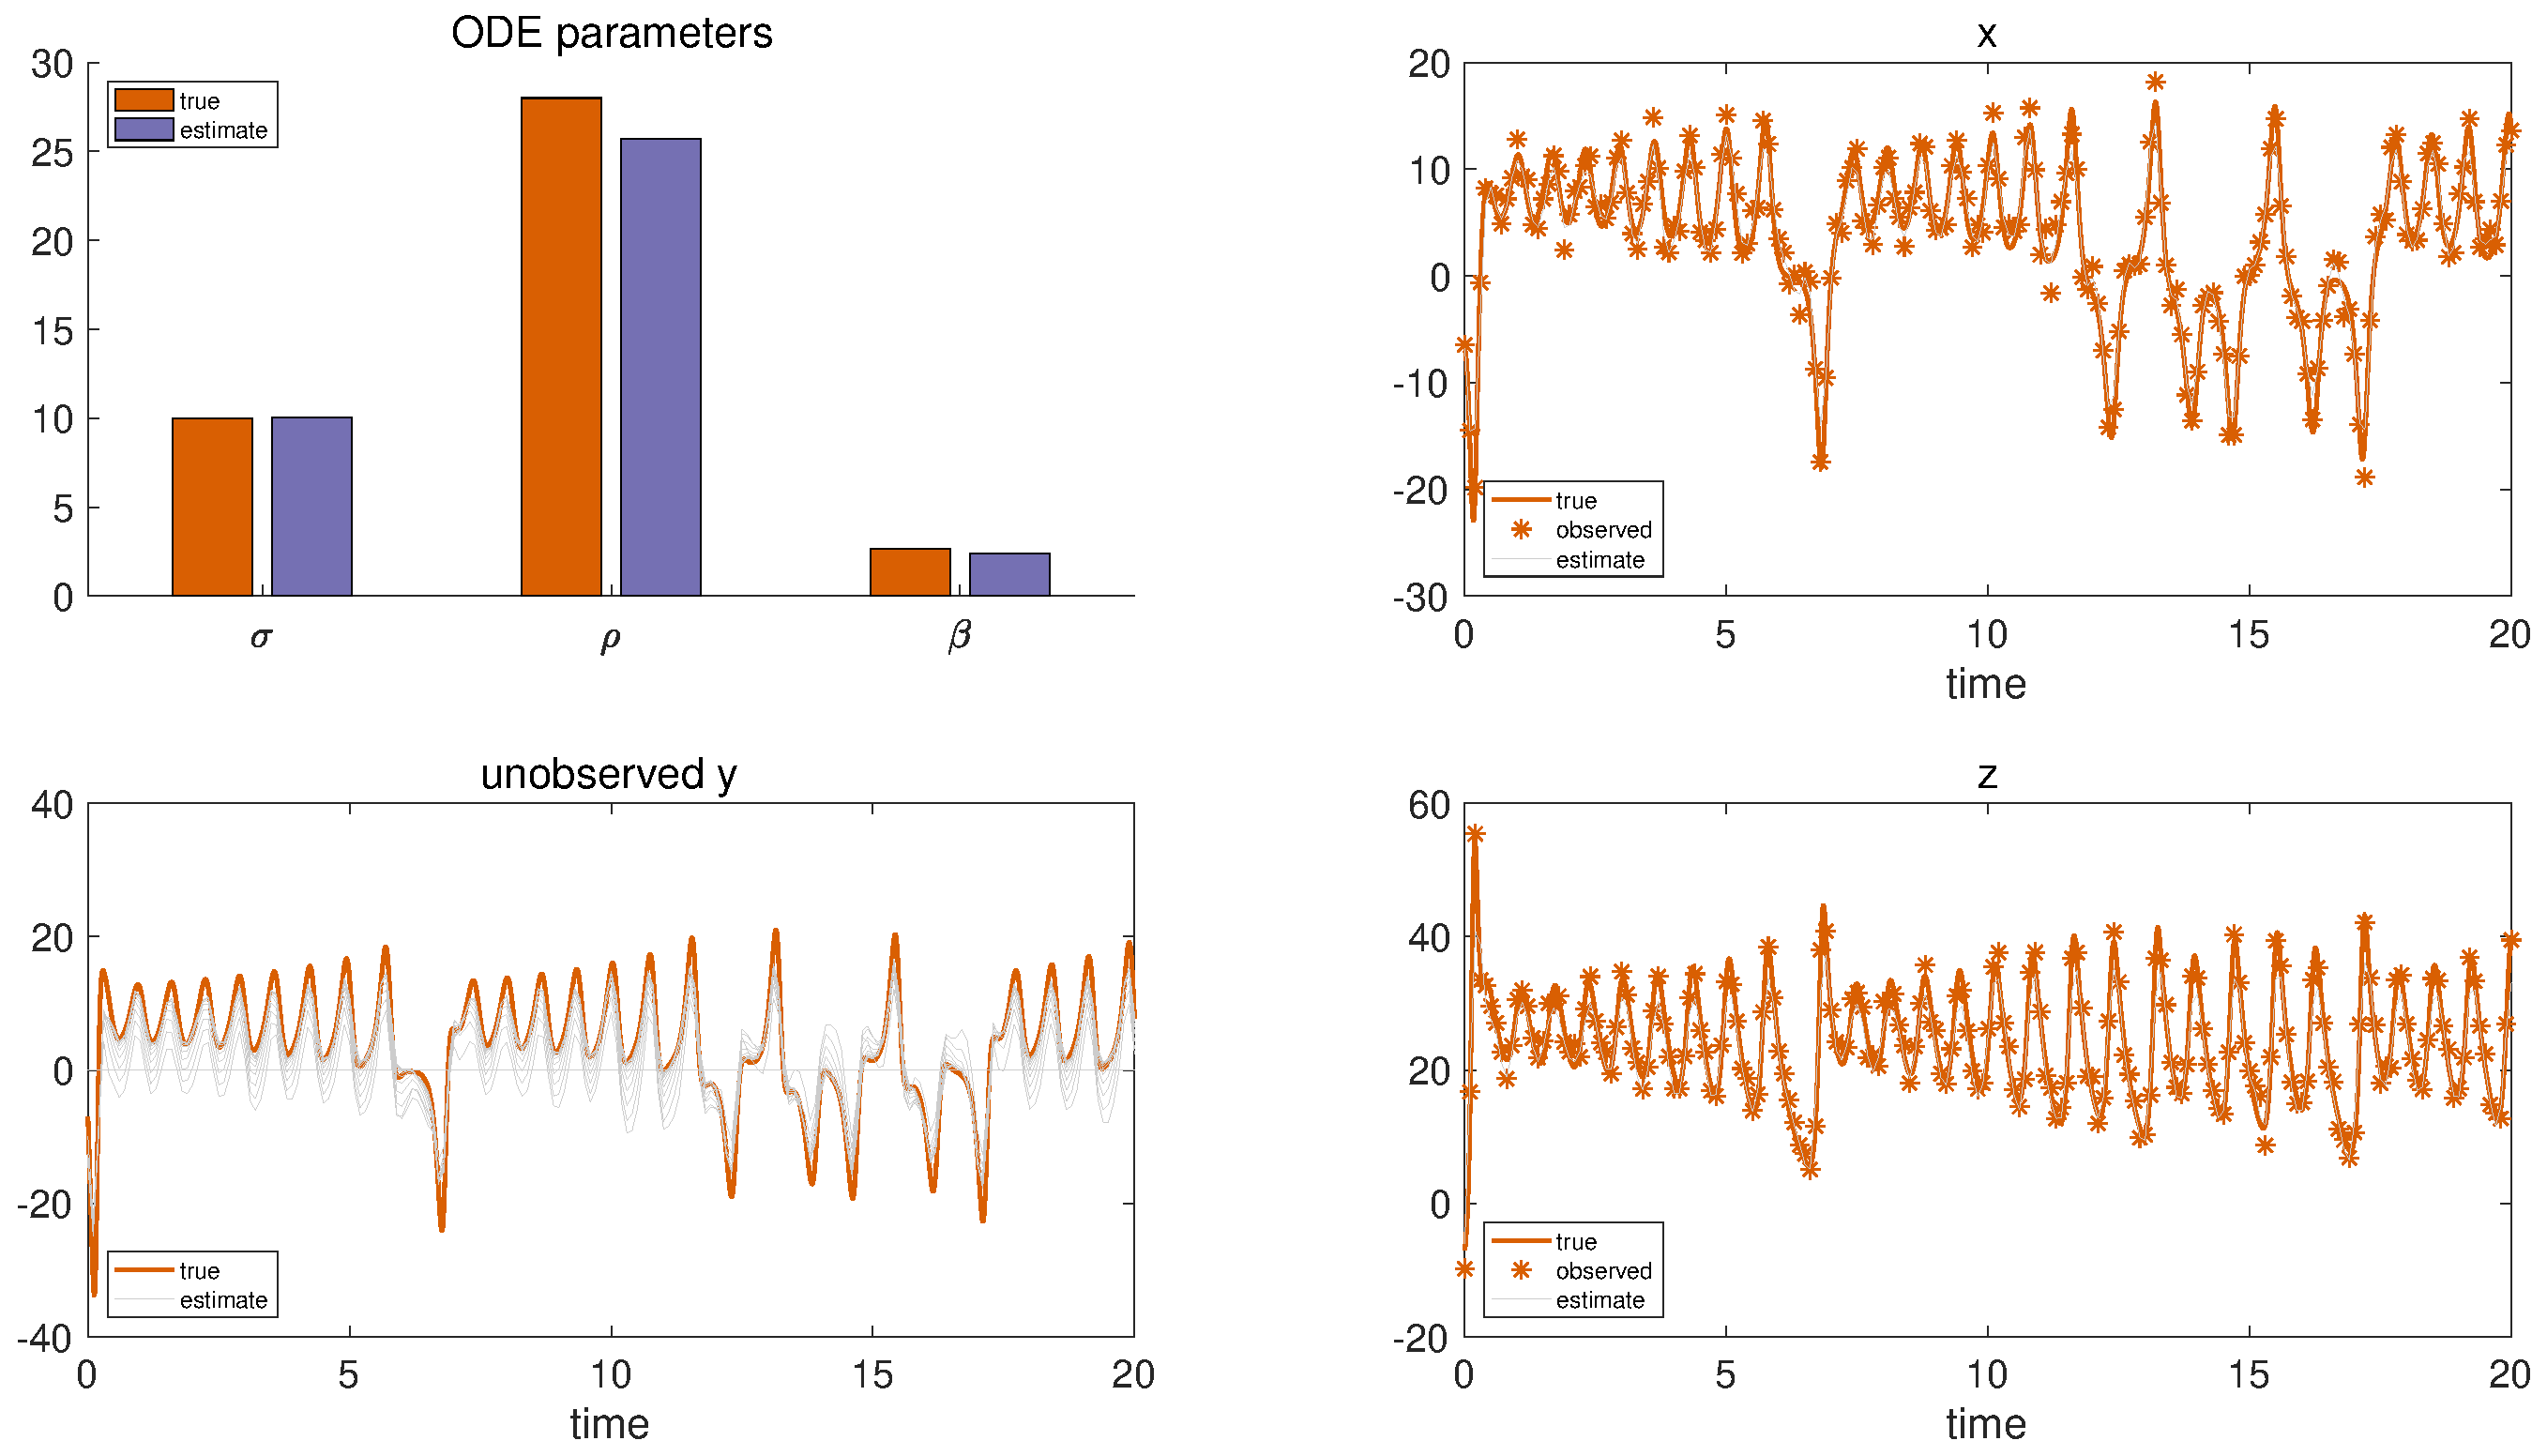
\includegraphics [width=4in]{Lorenz_attractor_4_30.eps}

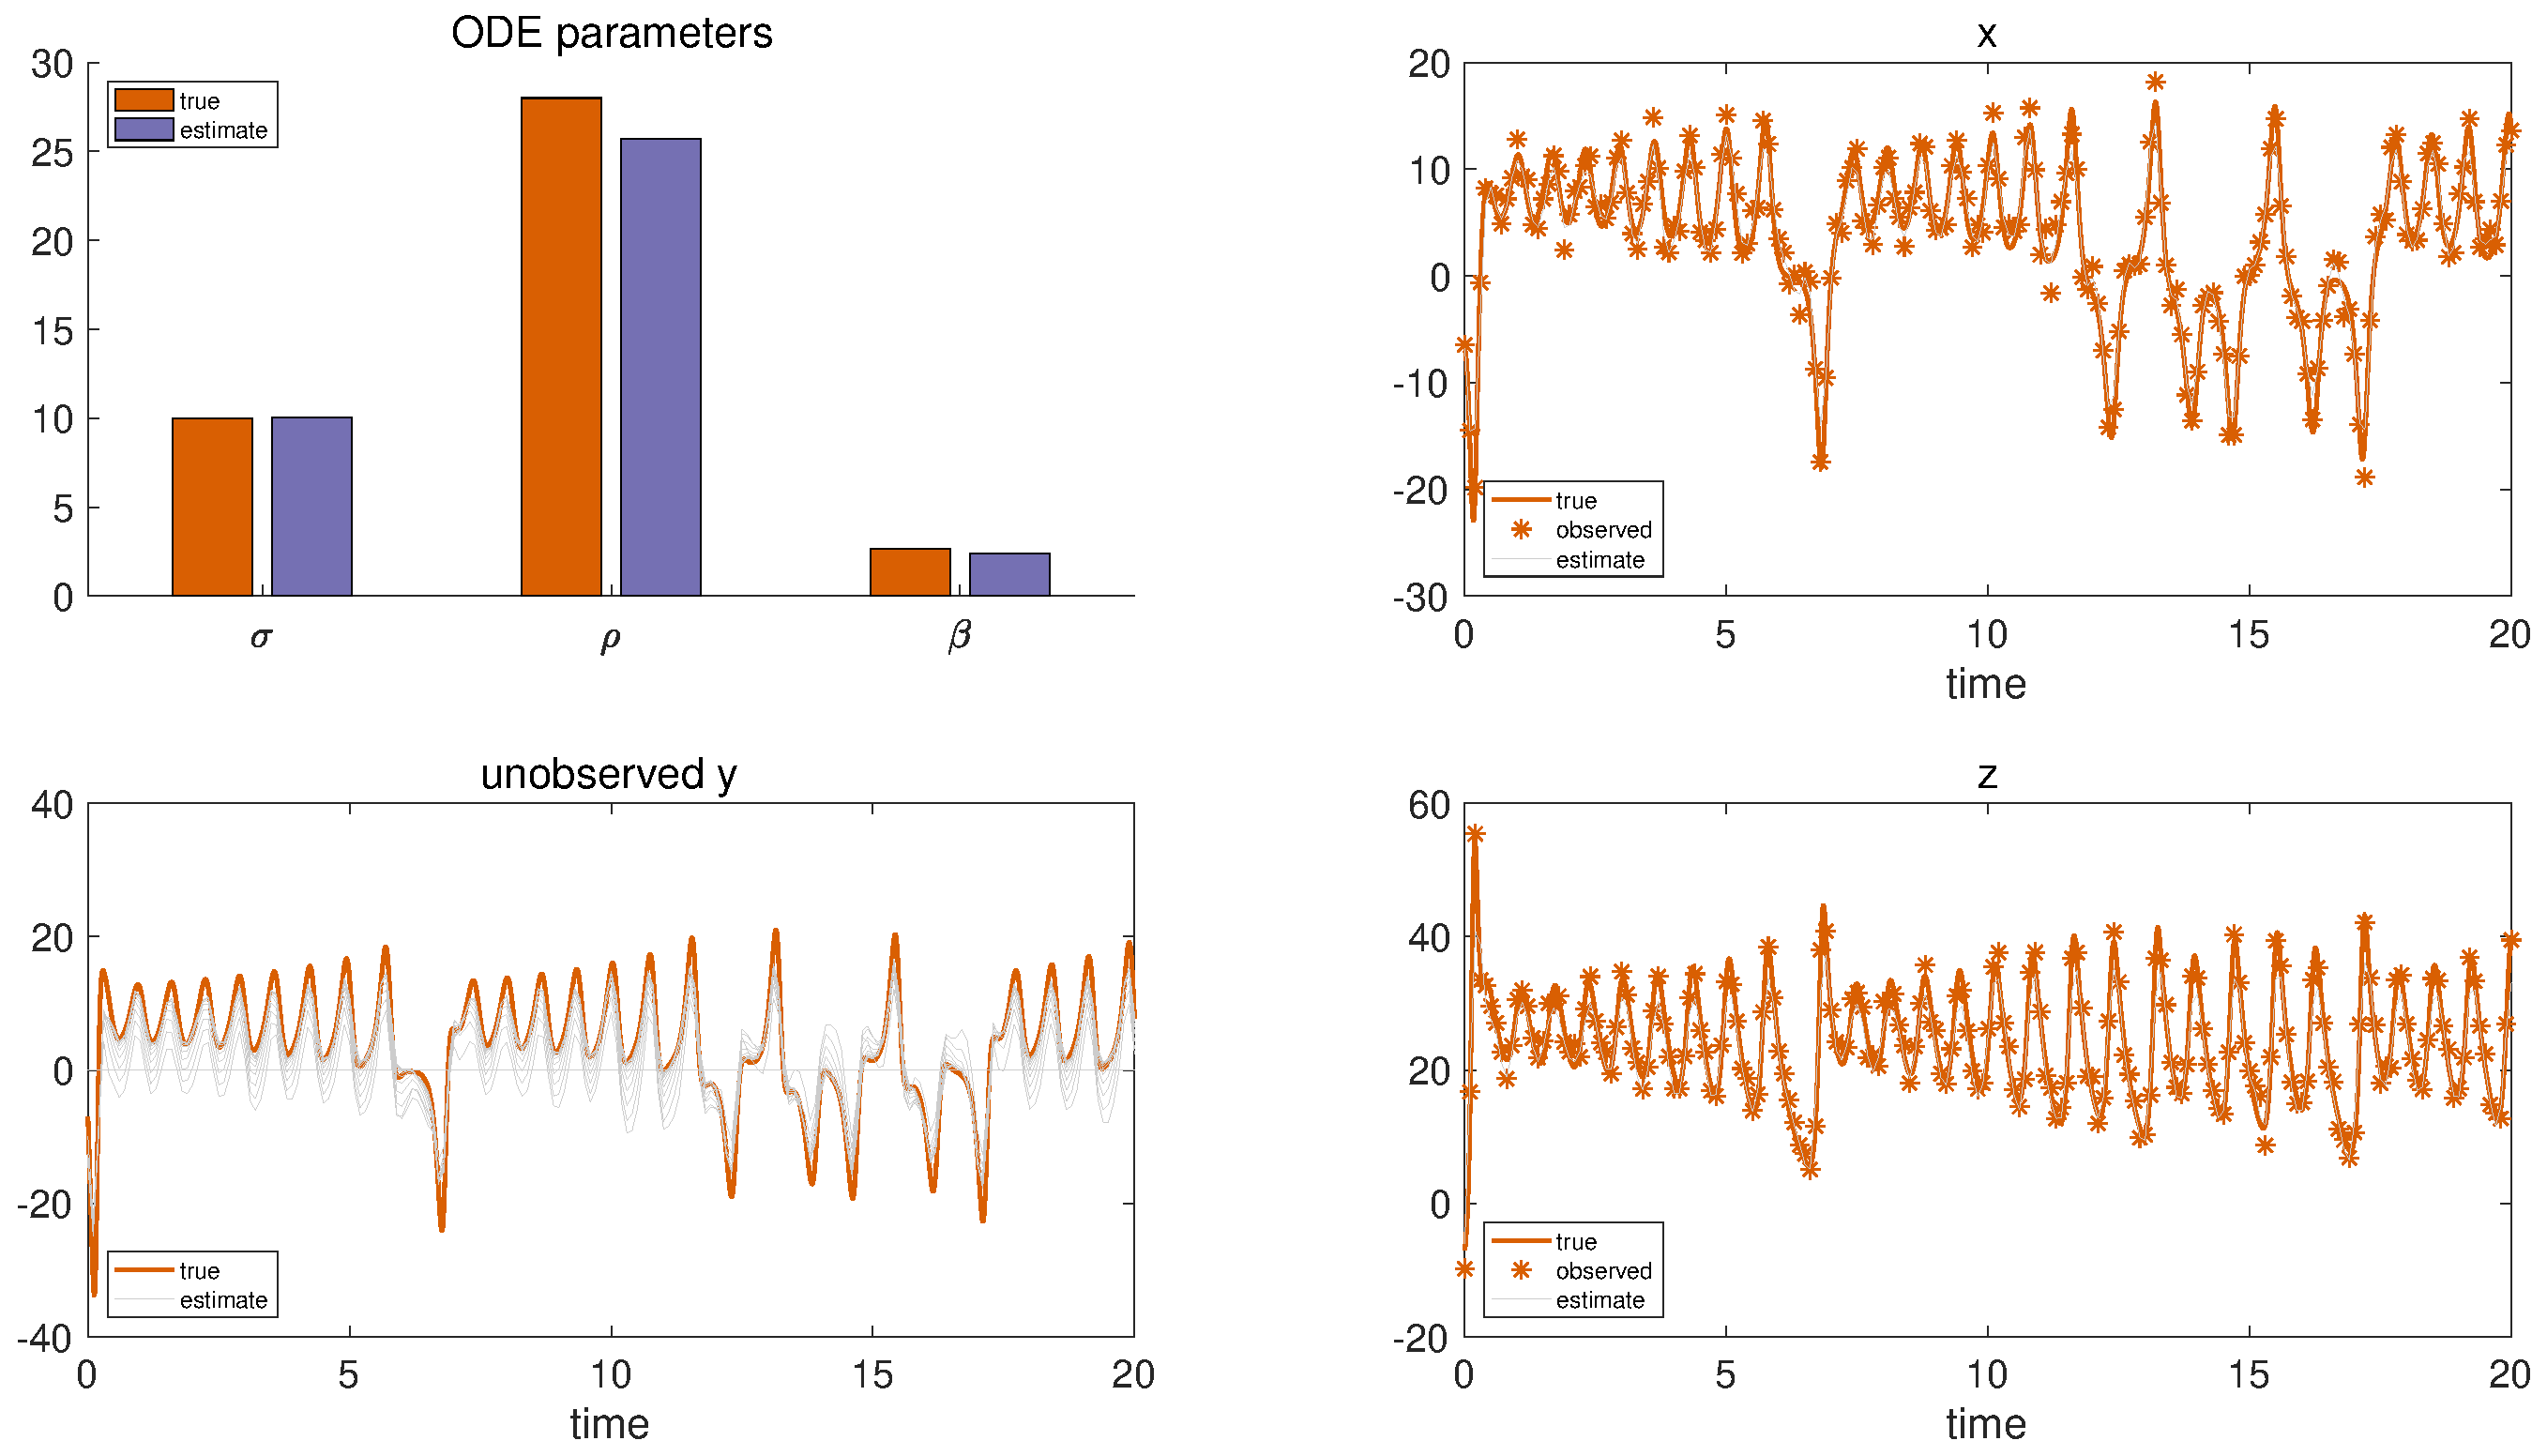
\includegraphics [width=4in]{Lorenz_attractor_4_31.eps}

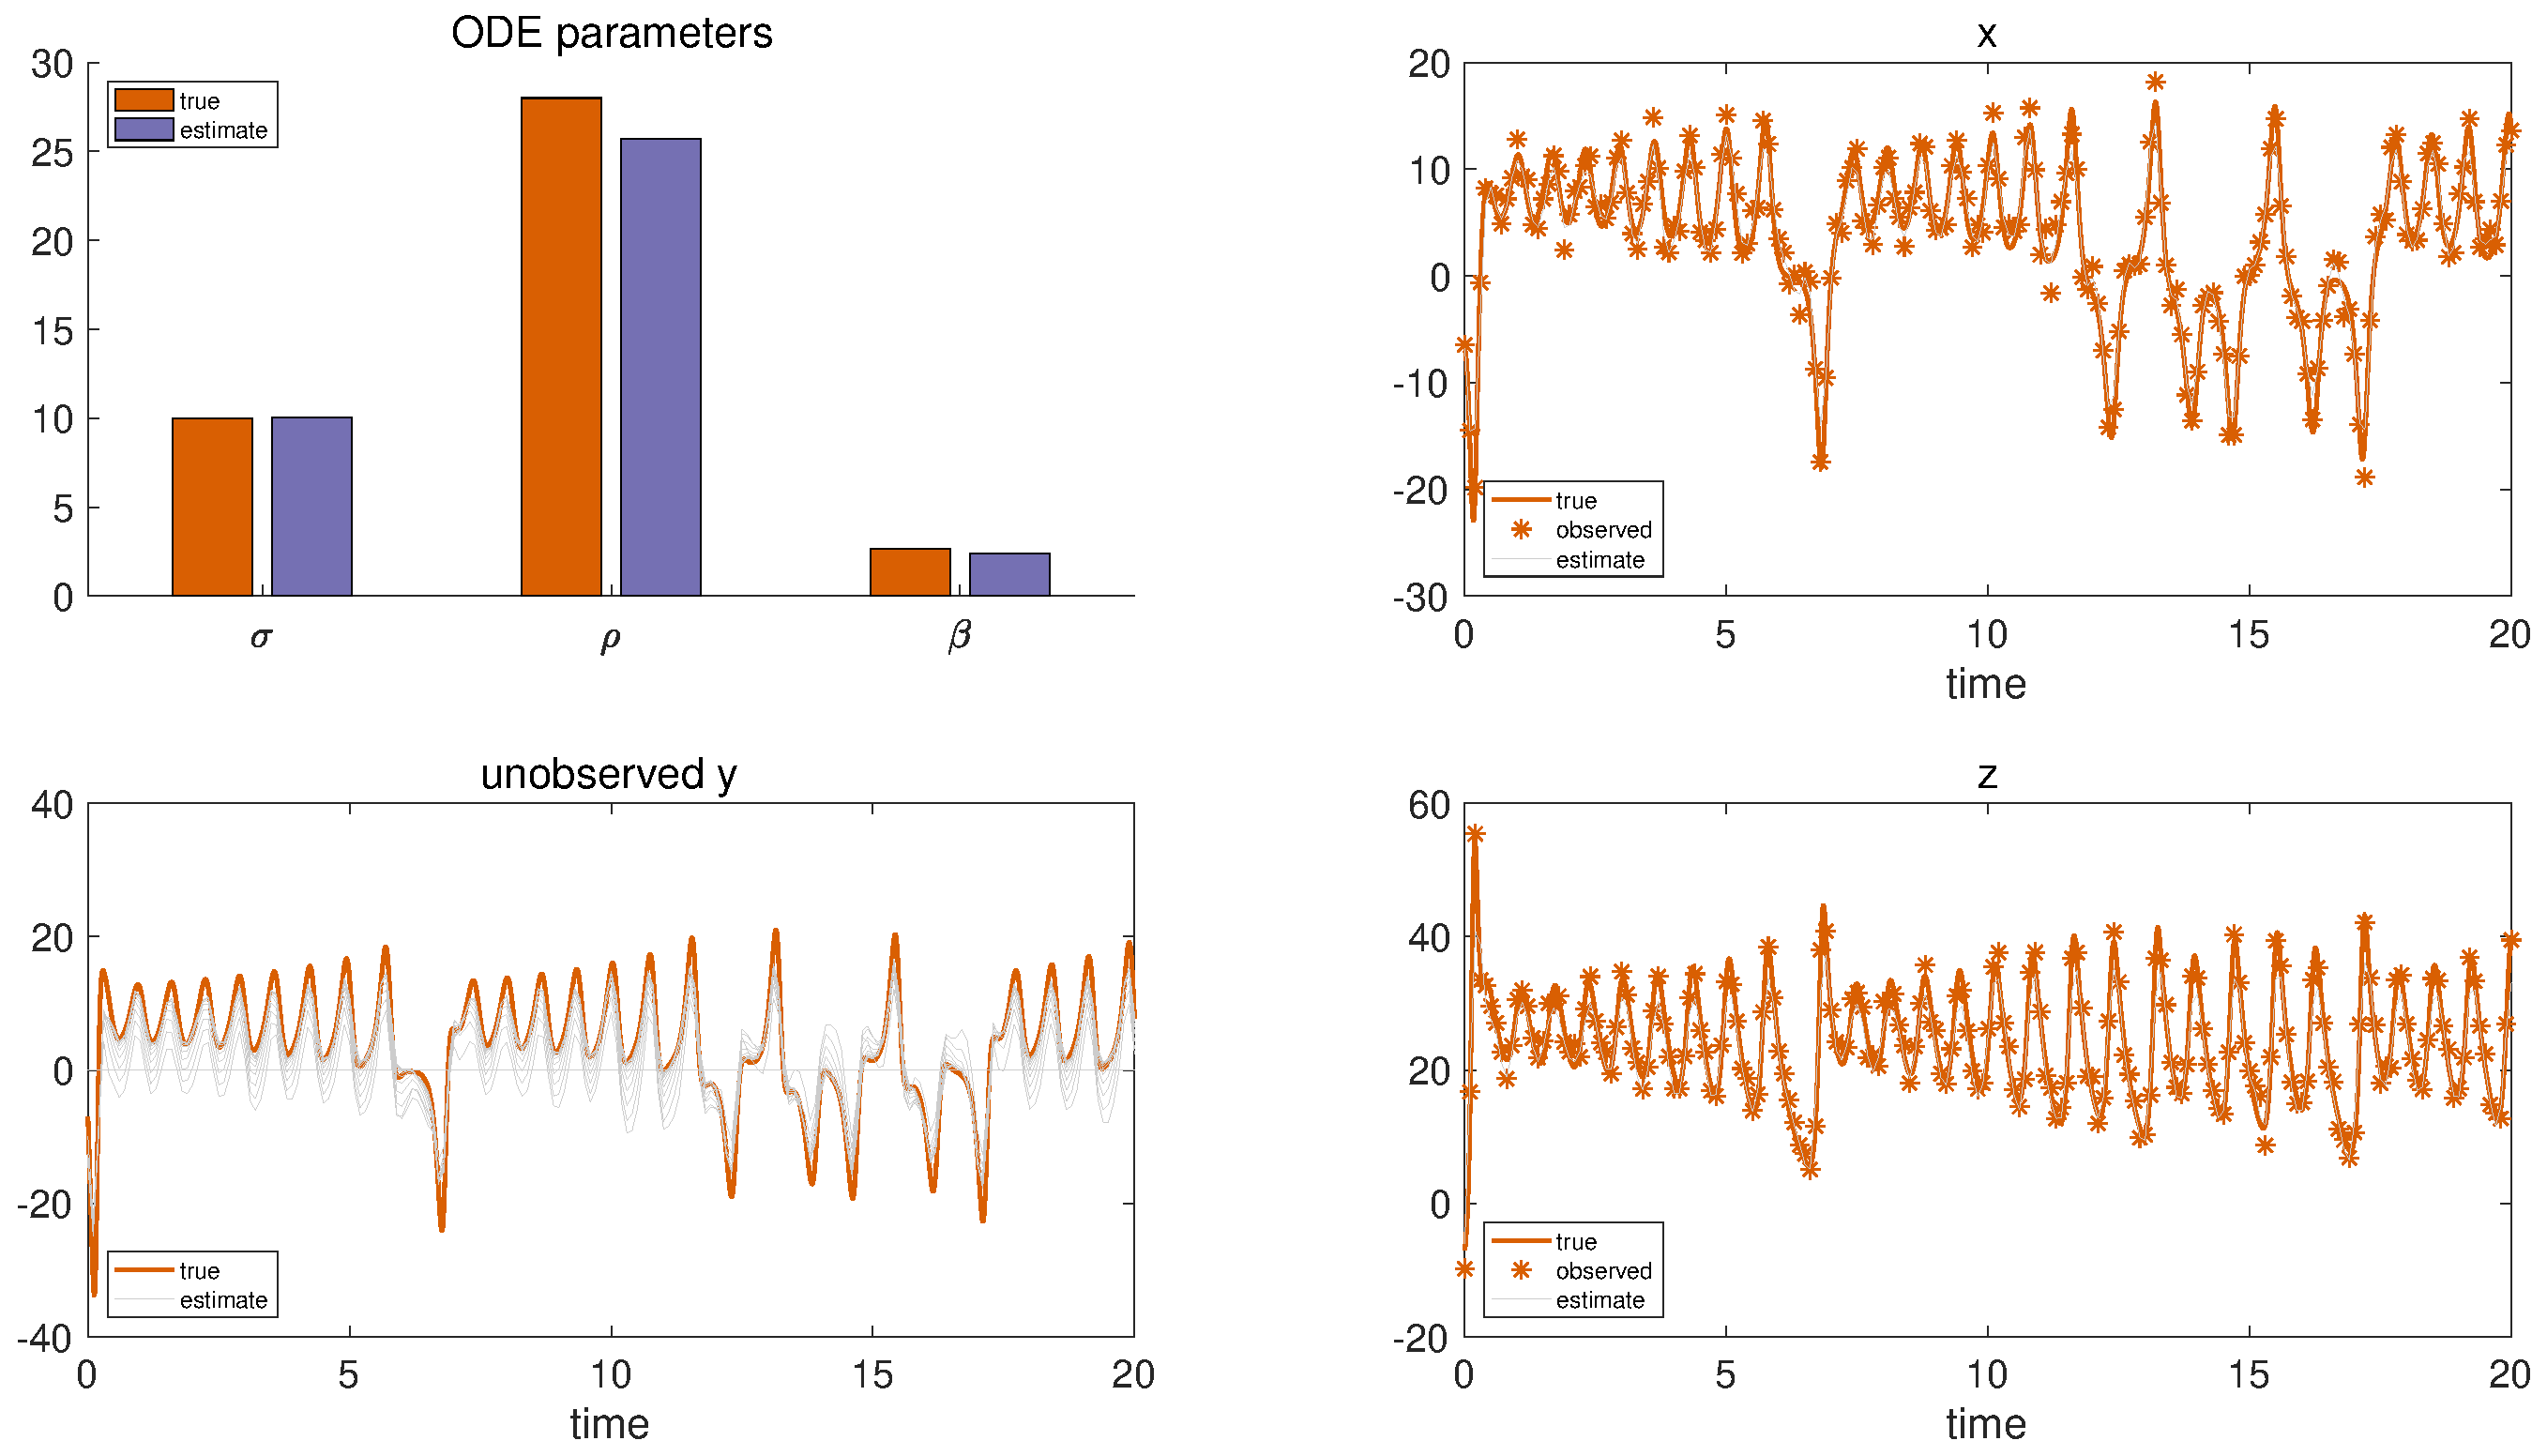
\includegraphics [width=4in]{Lorenz_attractor_4_32.eps}

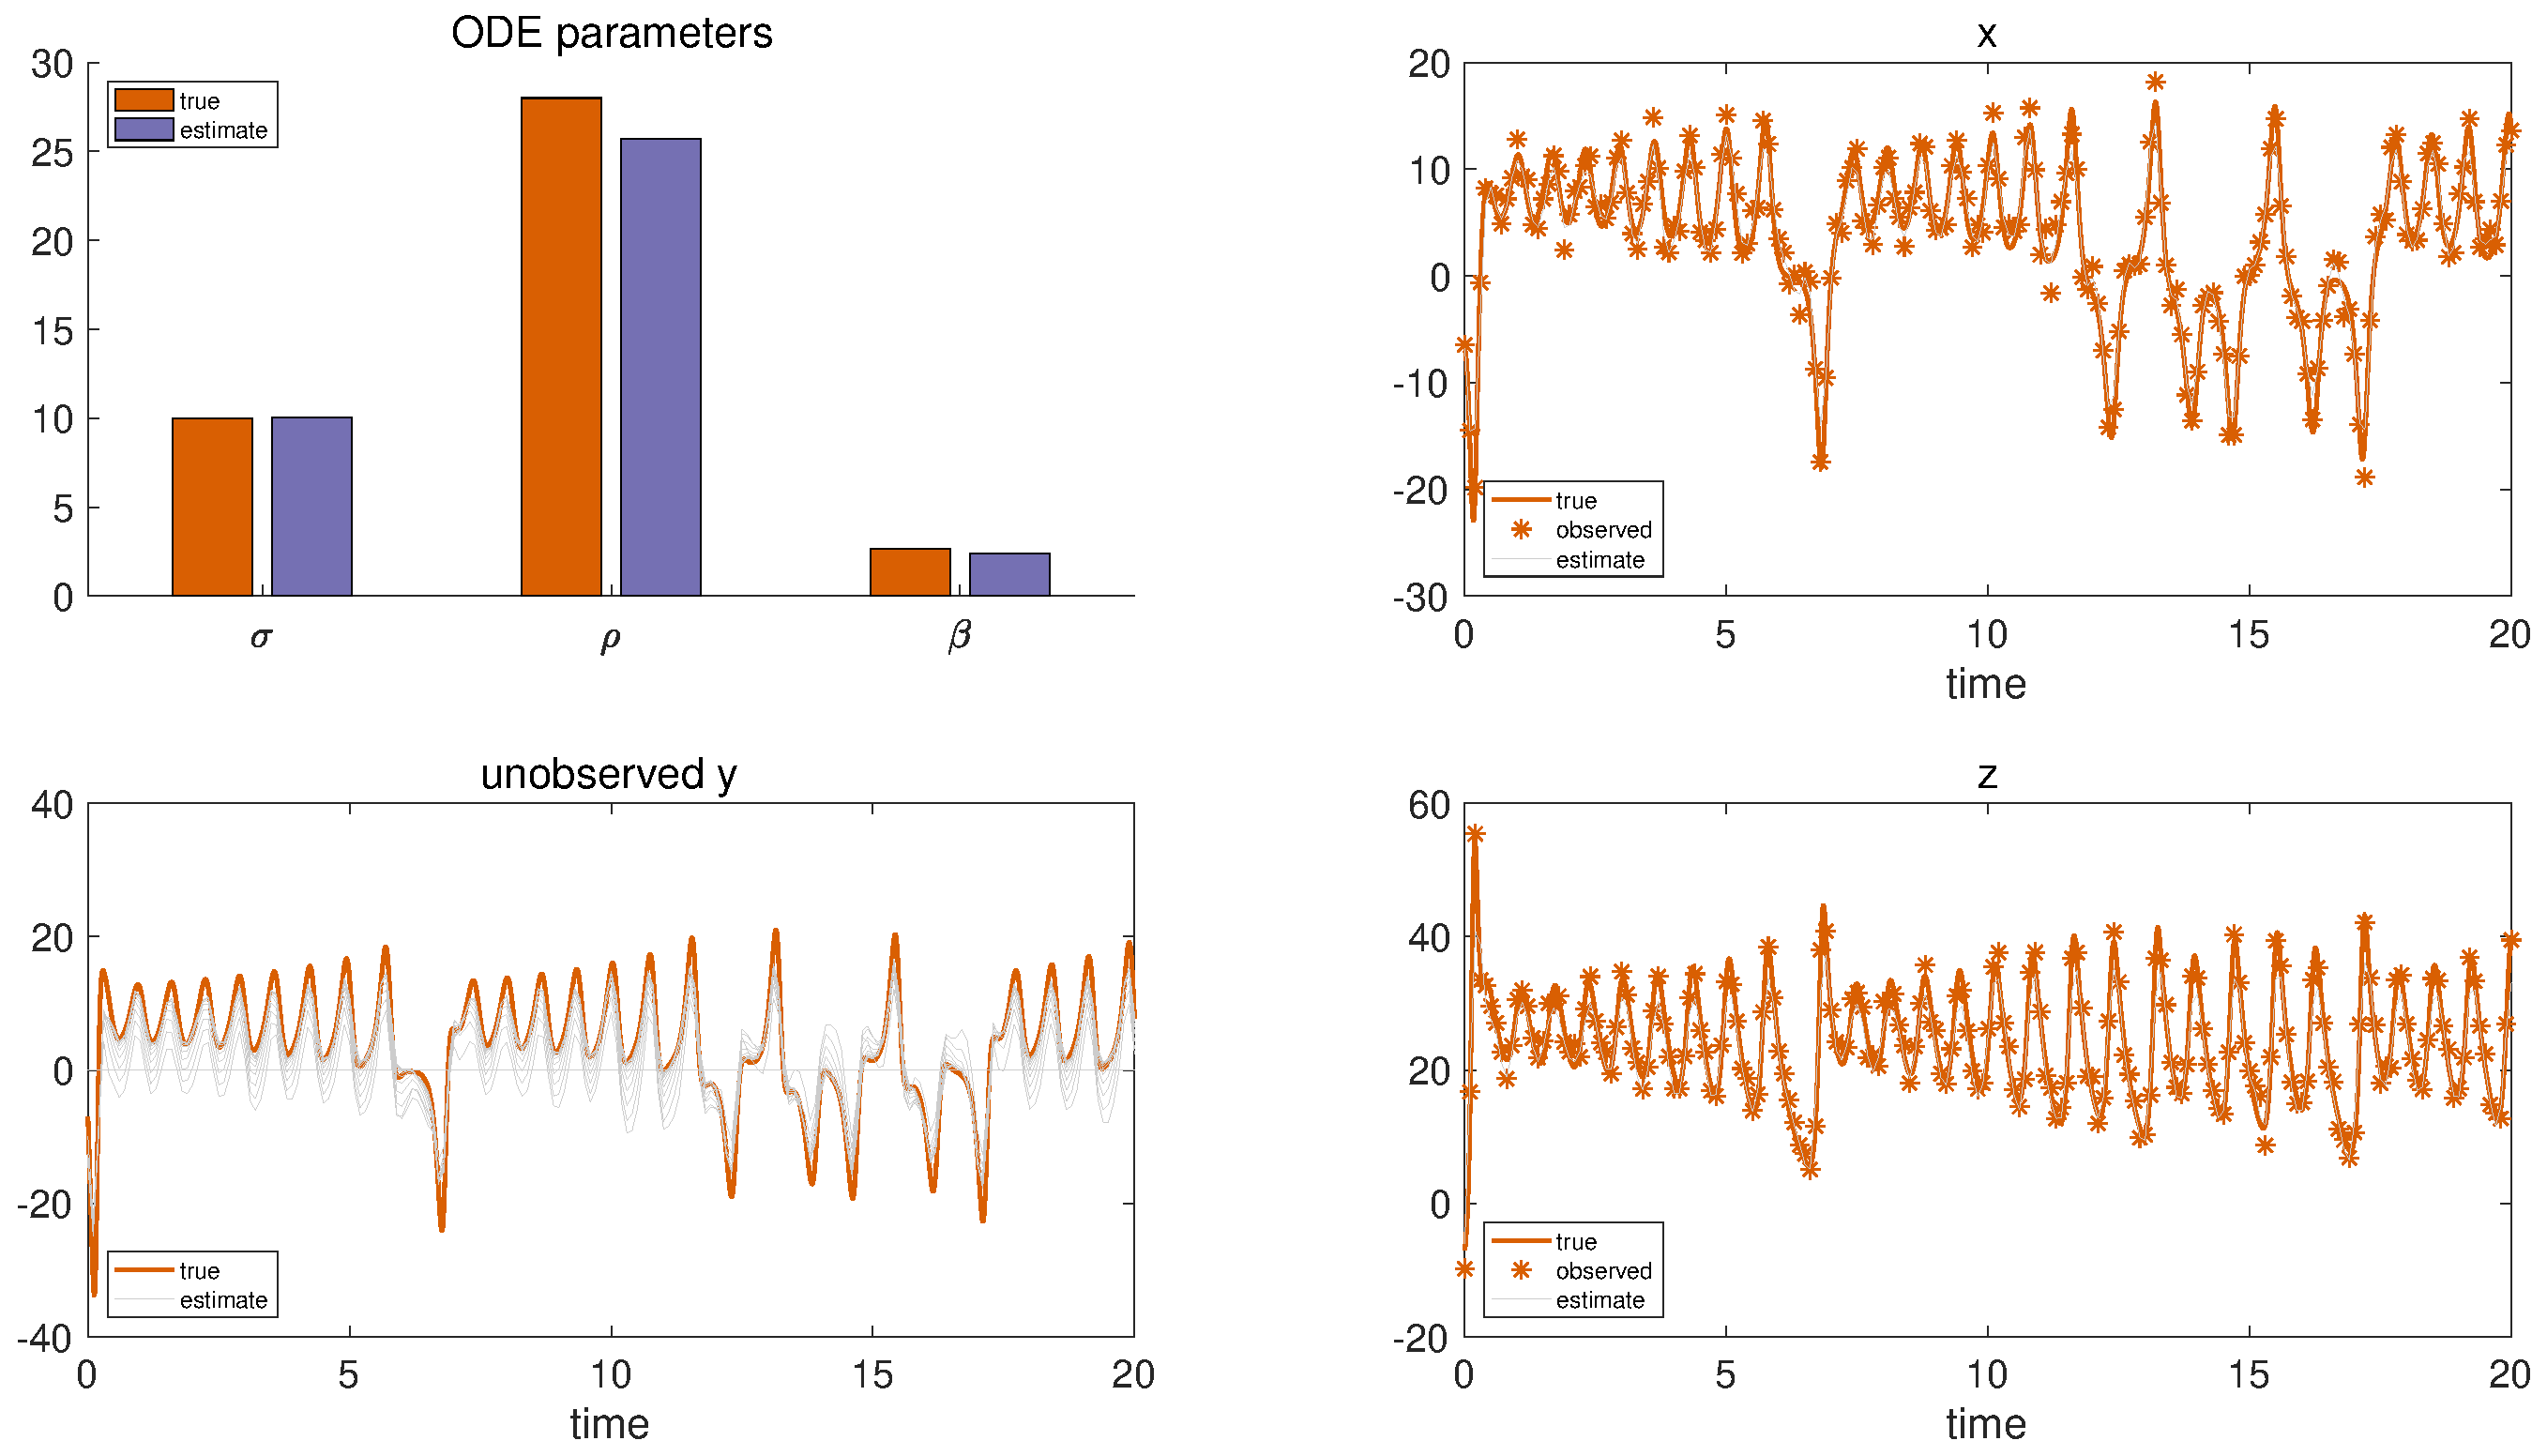
\includegraphics [width=4in]{Lorenz_attractor_4_33.eps}

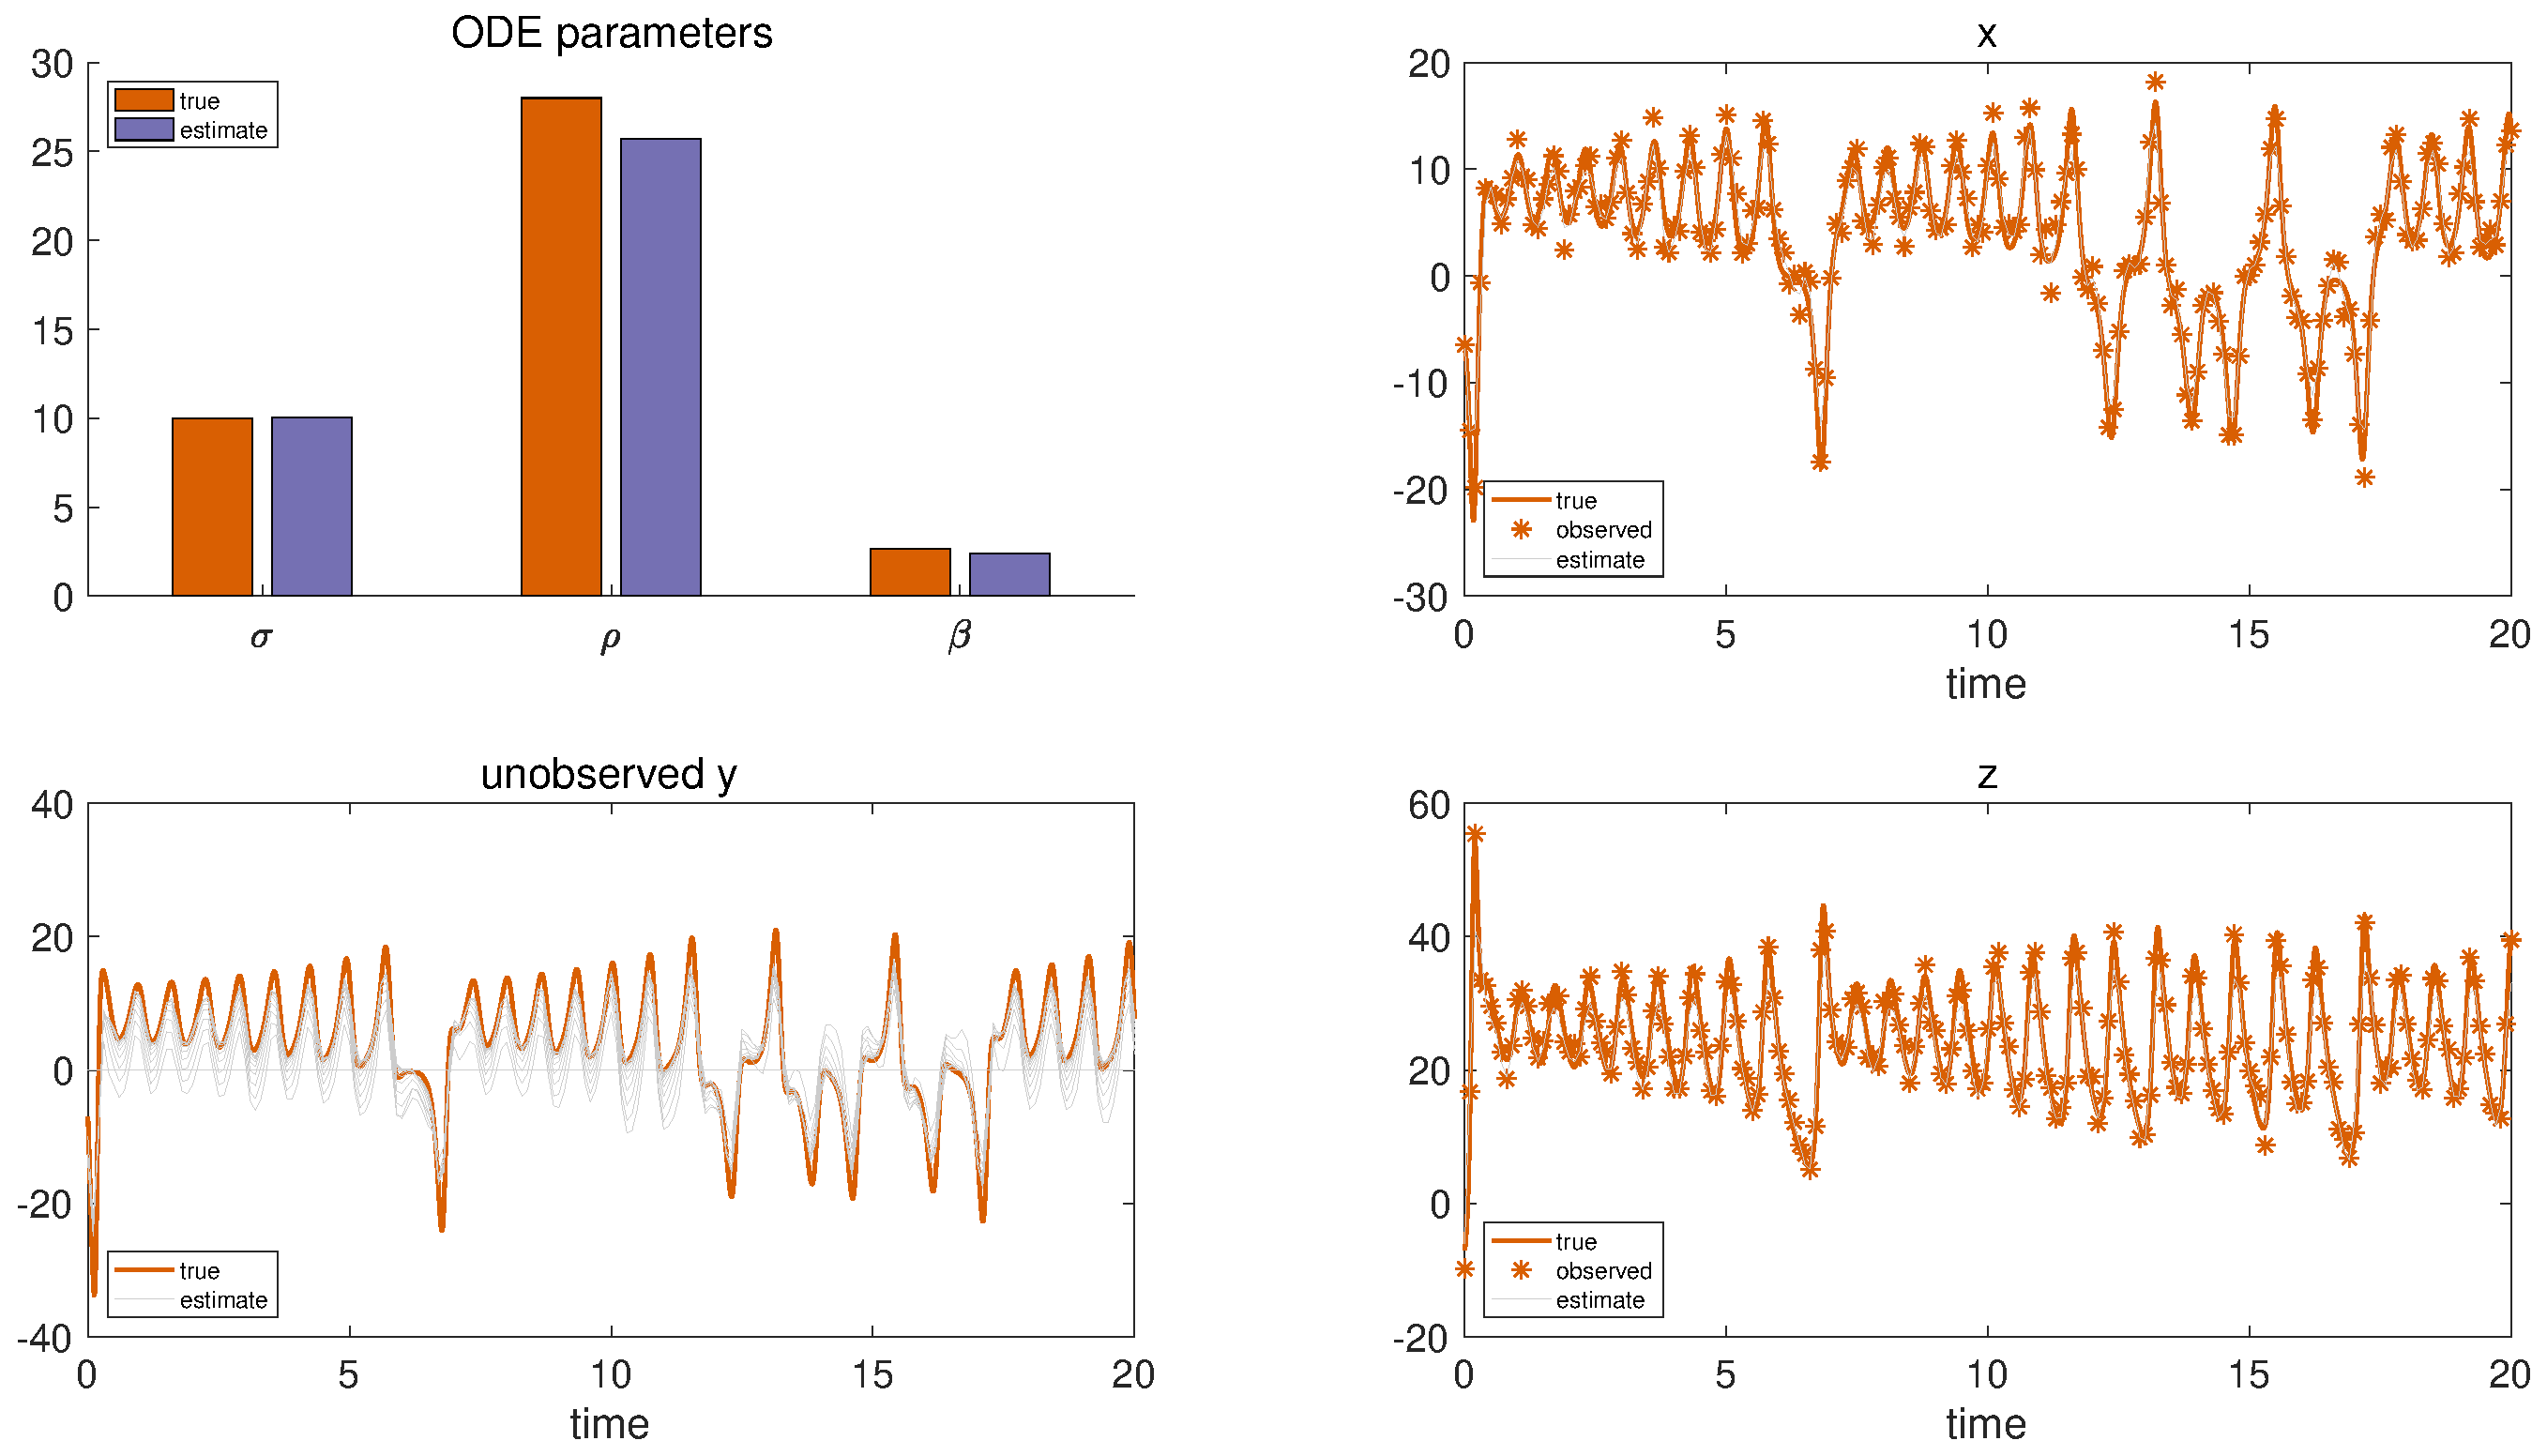
\includegraphics [width=4in]{Lorenz_attractor_4_34.eps}

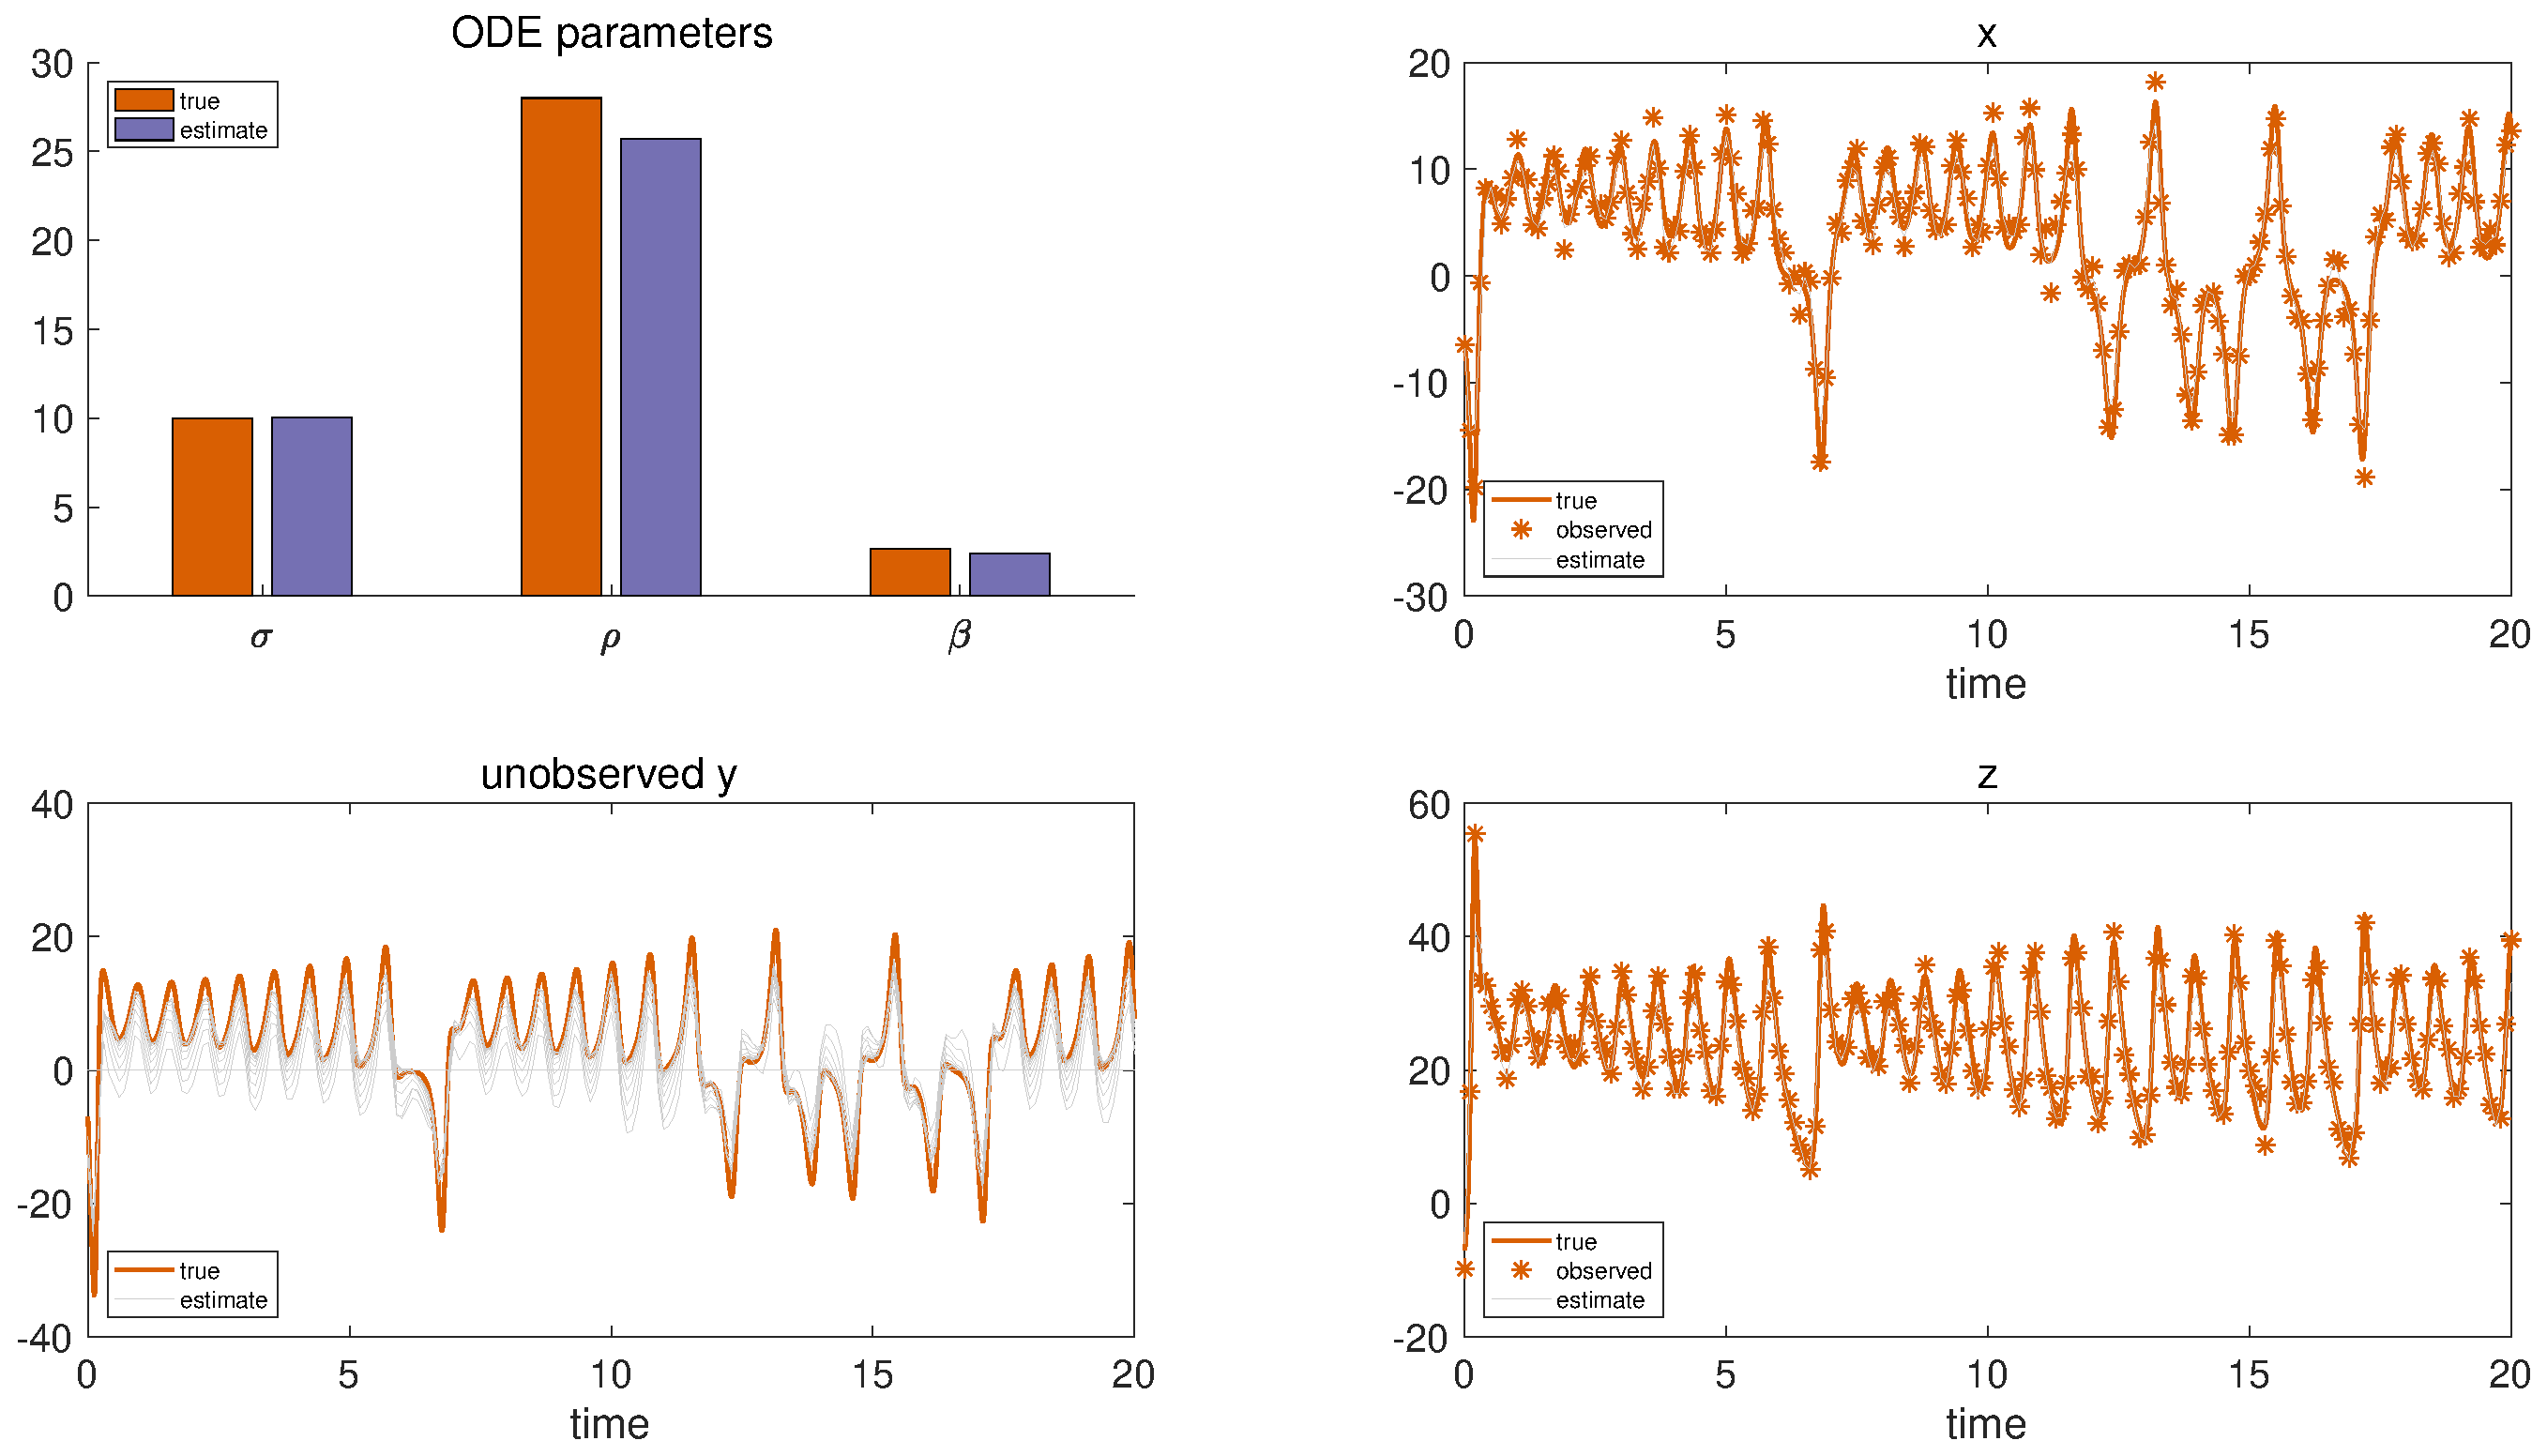
\includegraphics [width=4in]{Lorenz_attractor_4_35.eps}

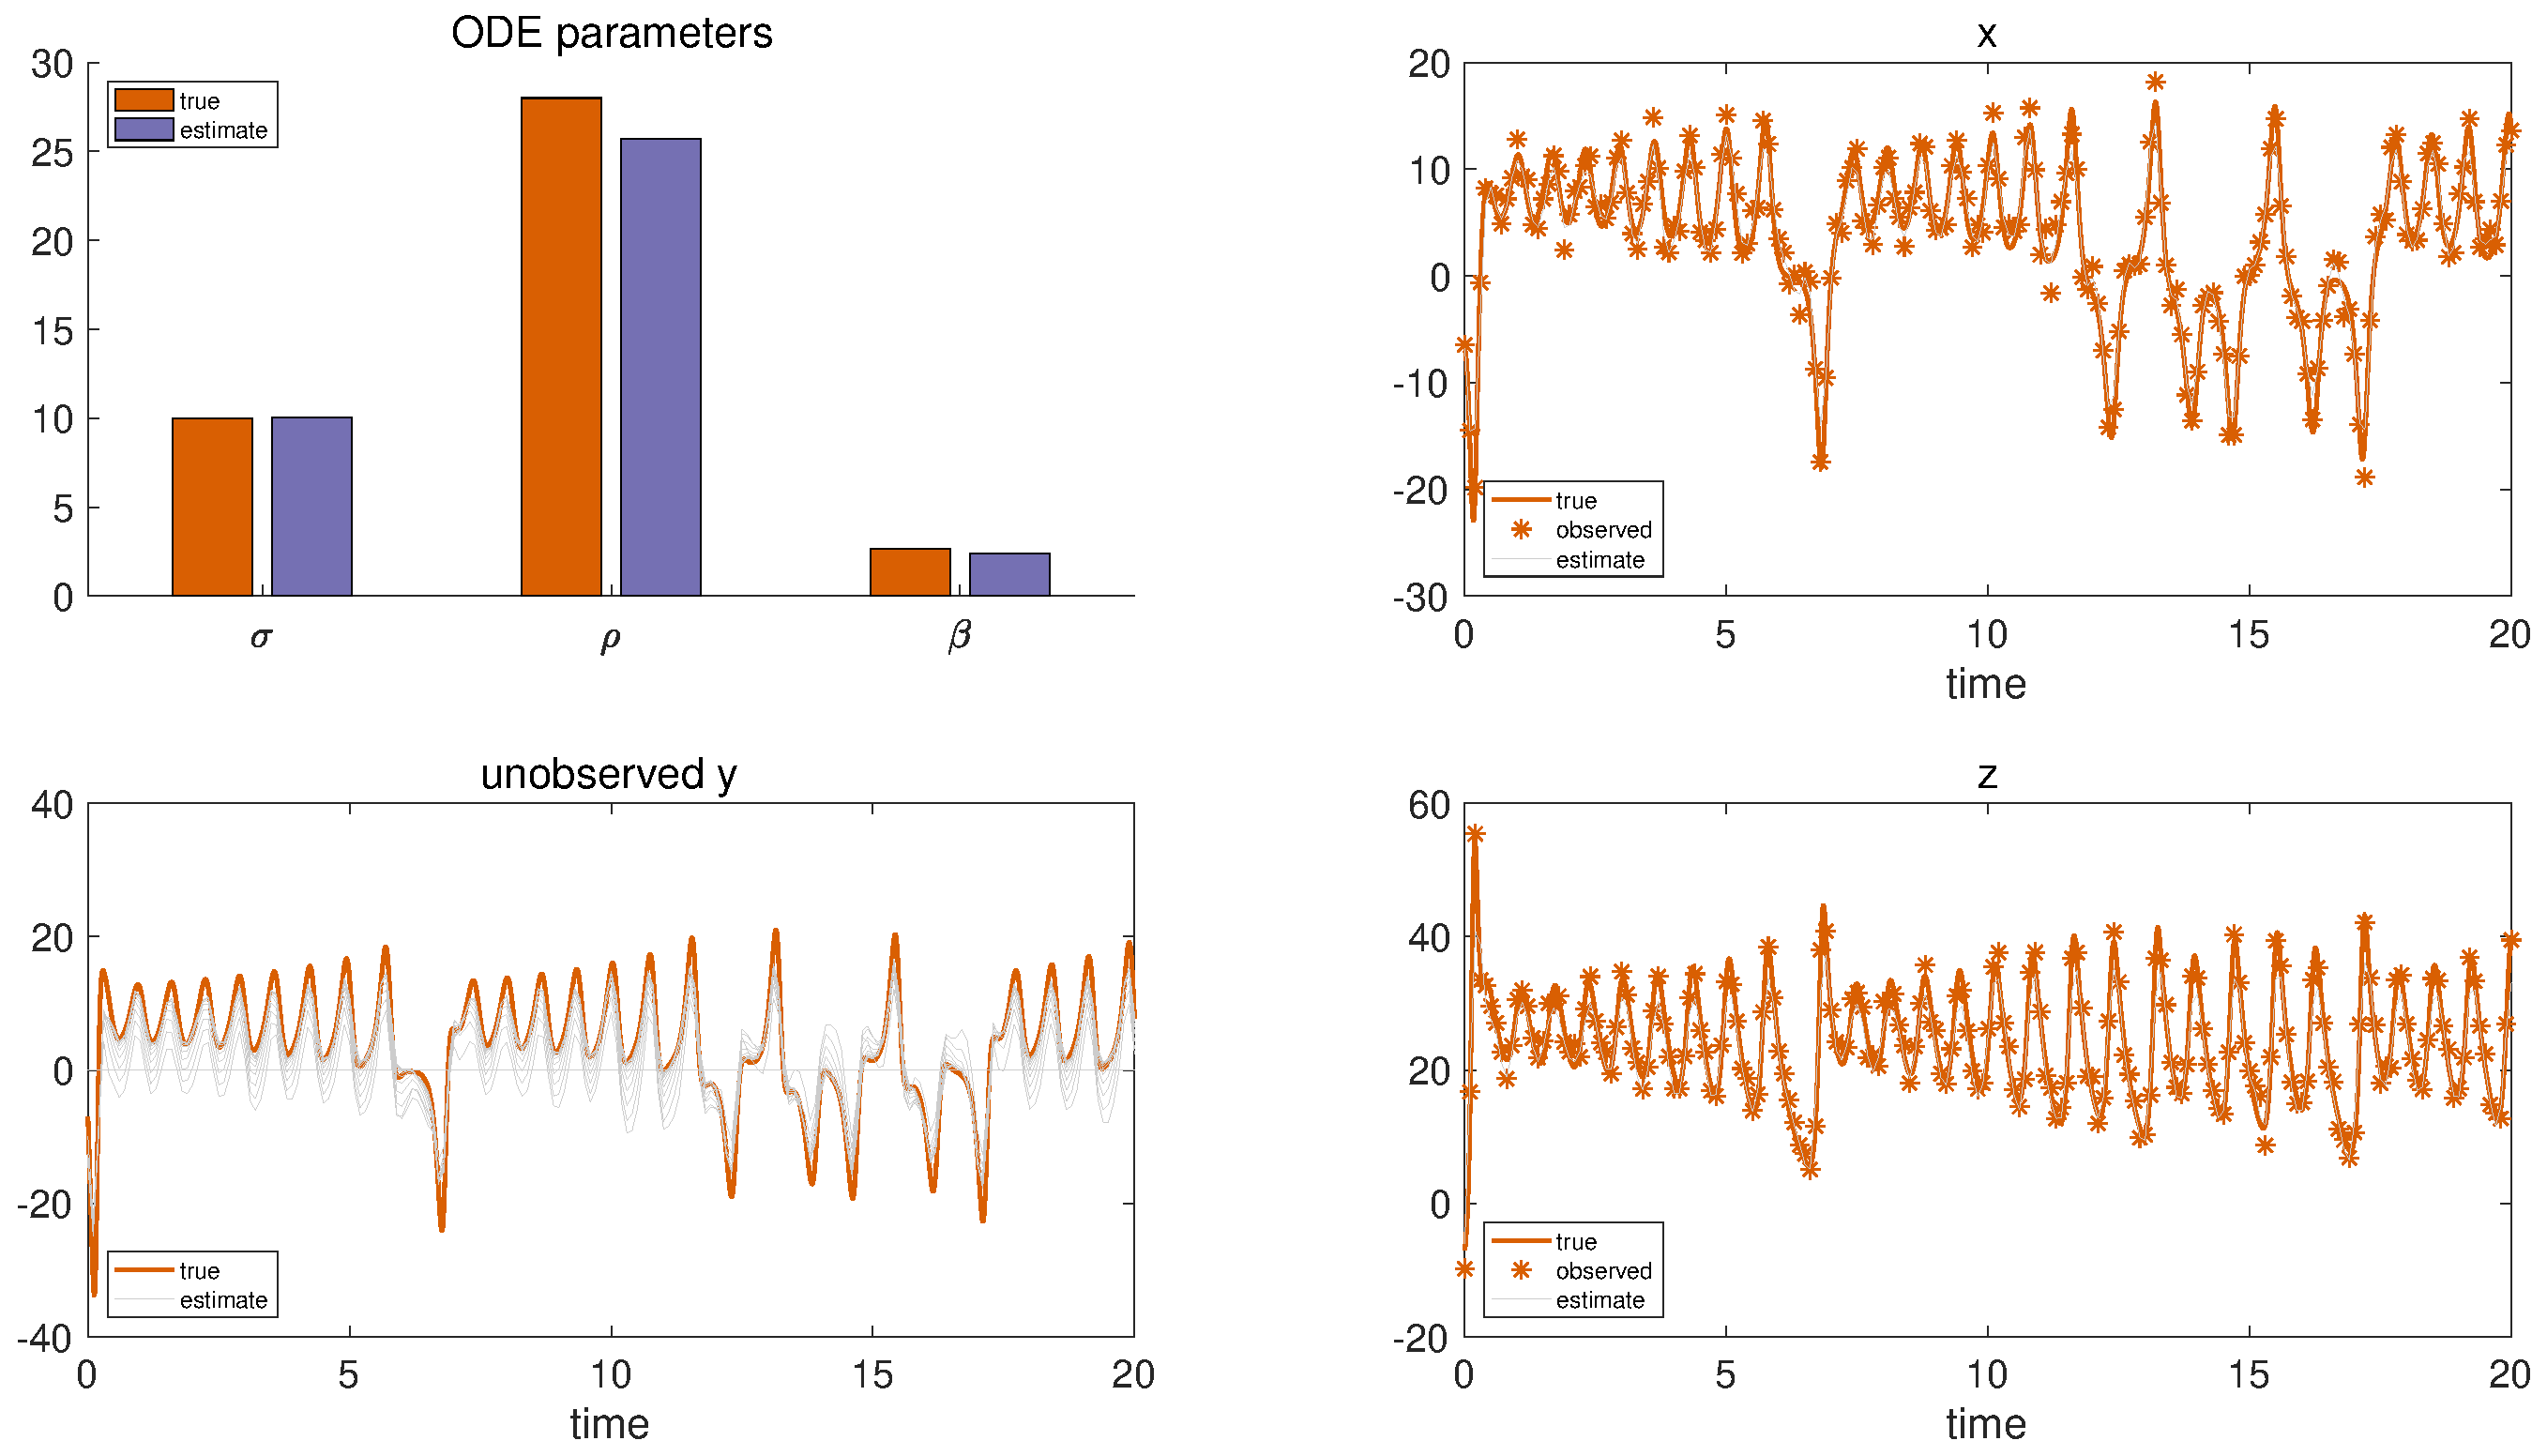
\includegraphics [width=4in]{Lorenz_attractor_4_36.eps}

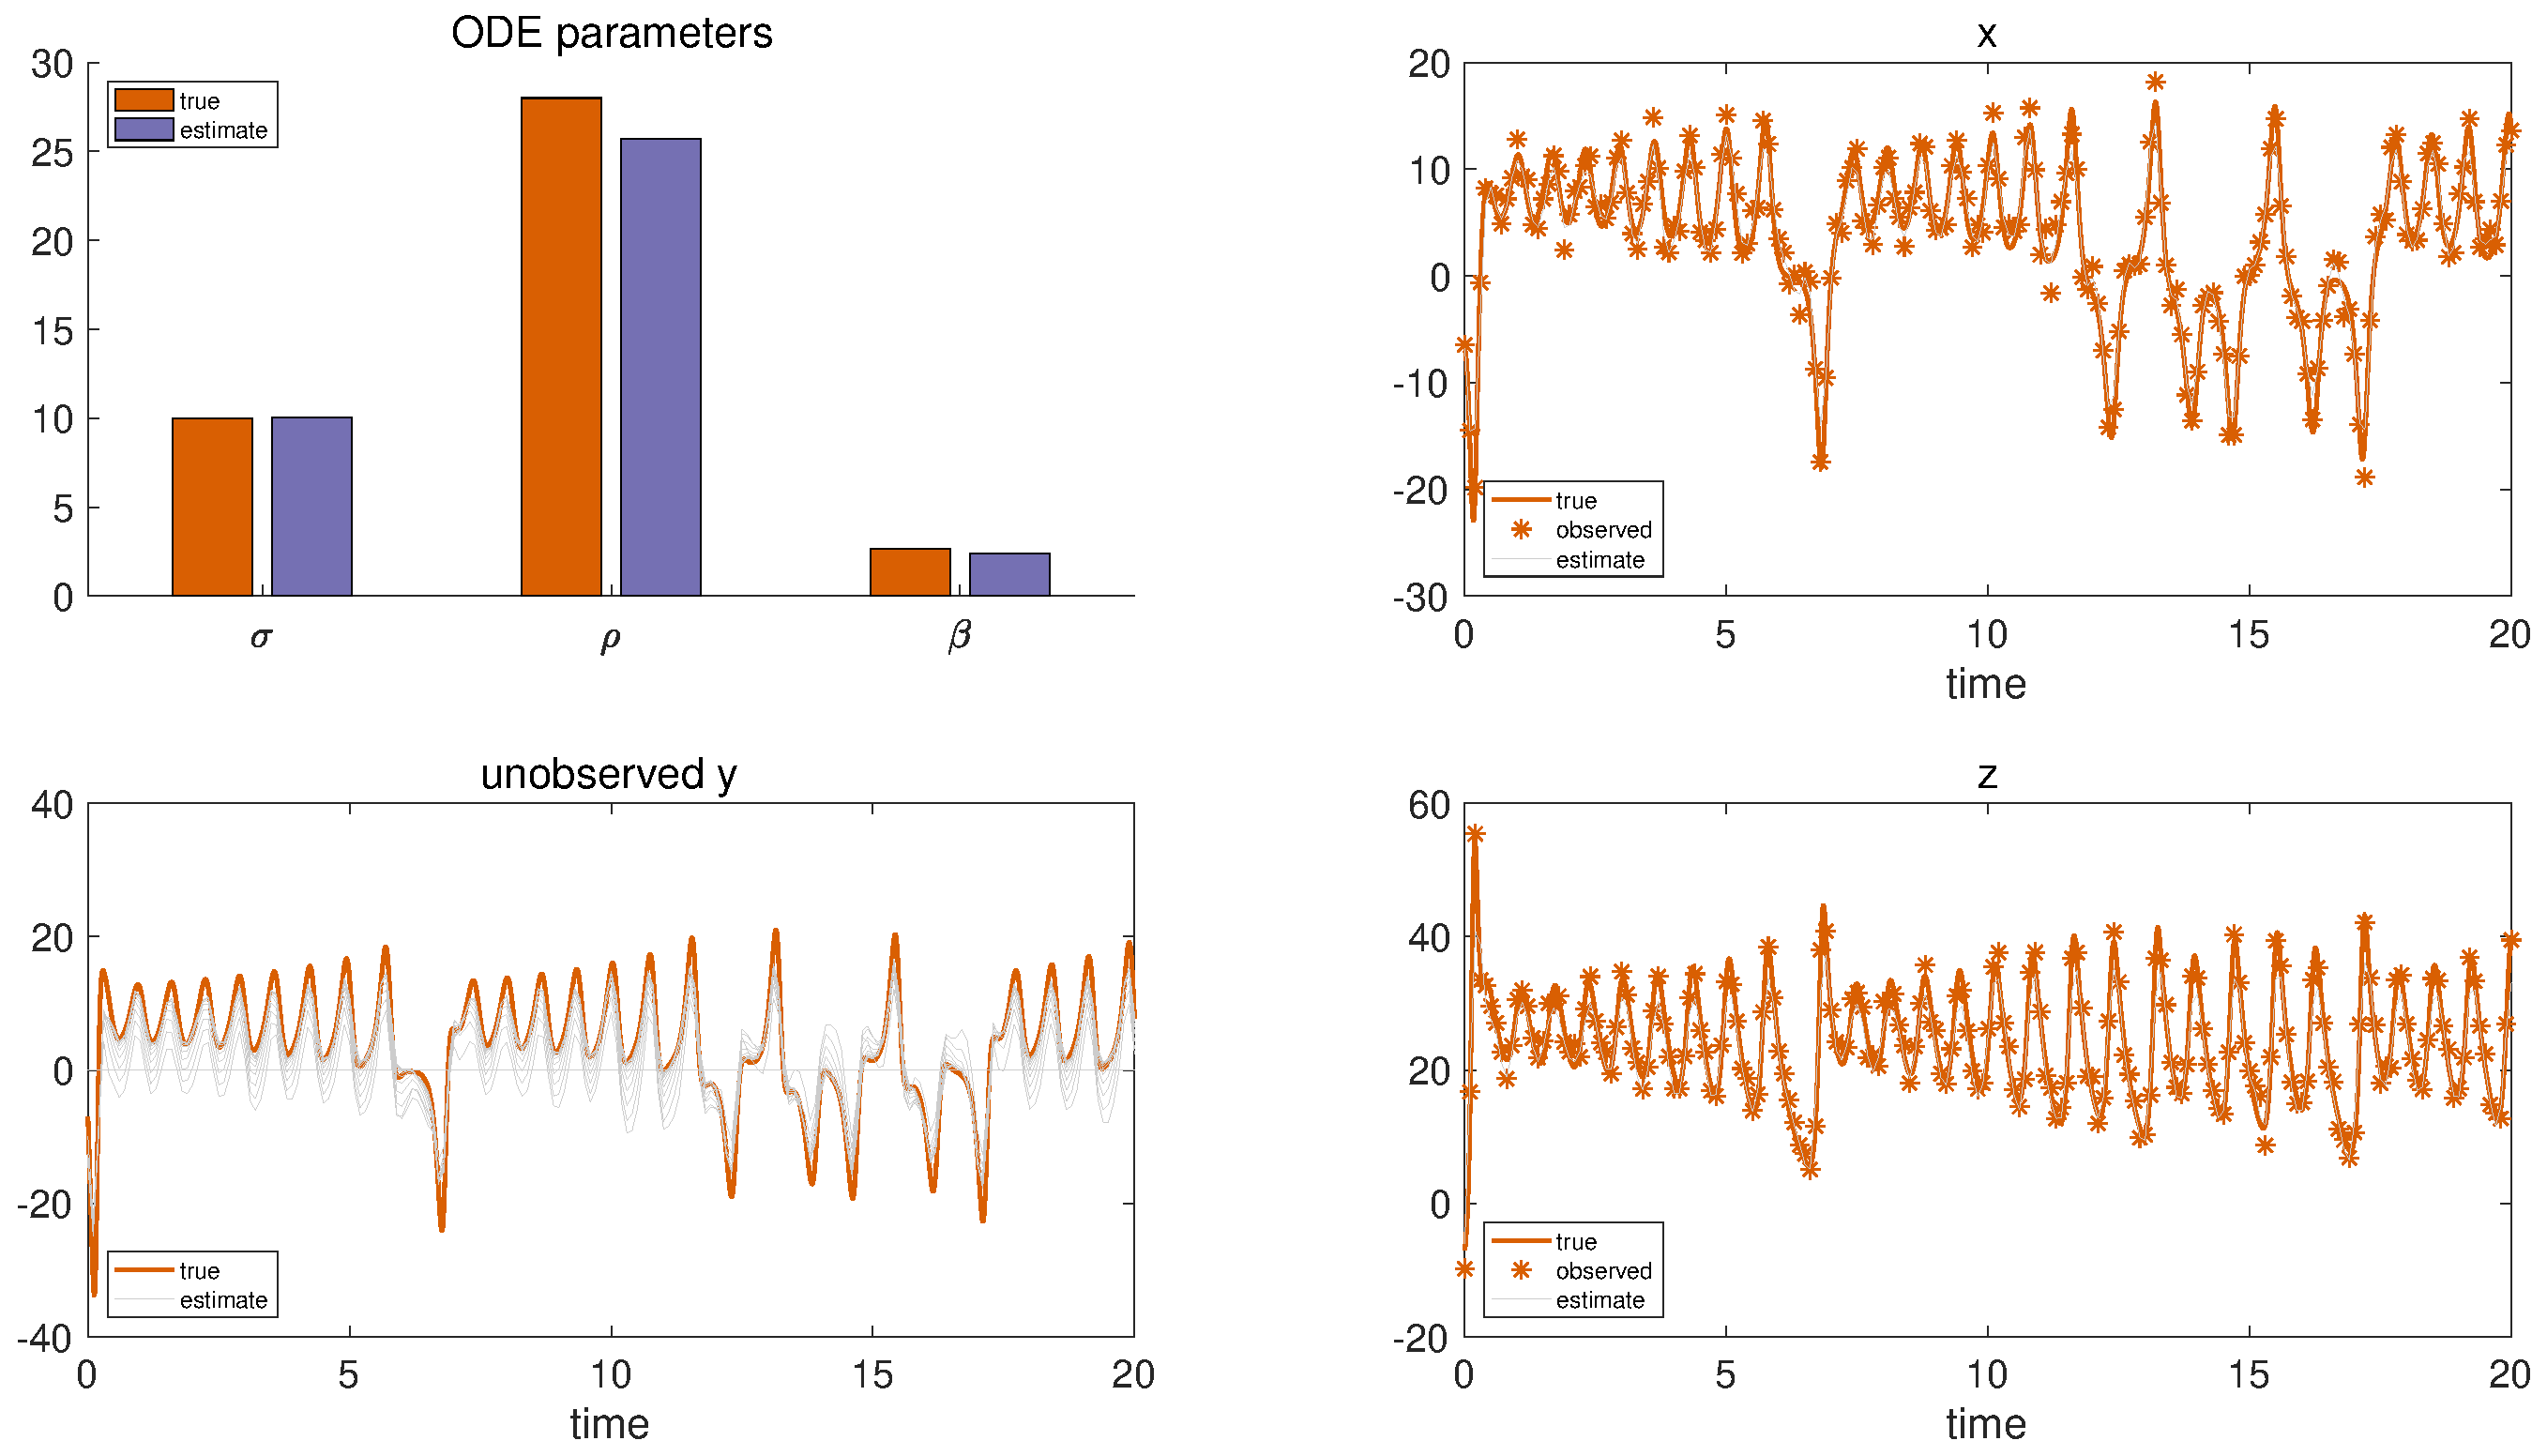
\includegraphics [width=4in]{Lorenz_attractor_4_37.eps}

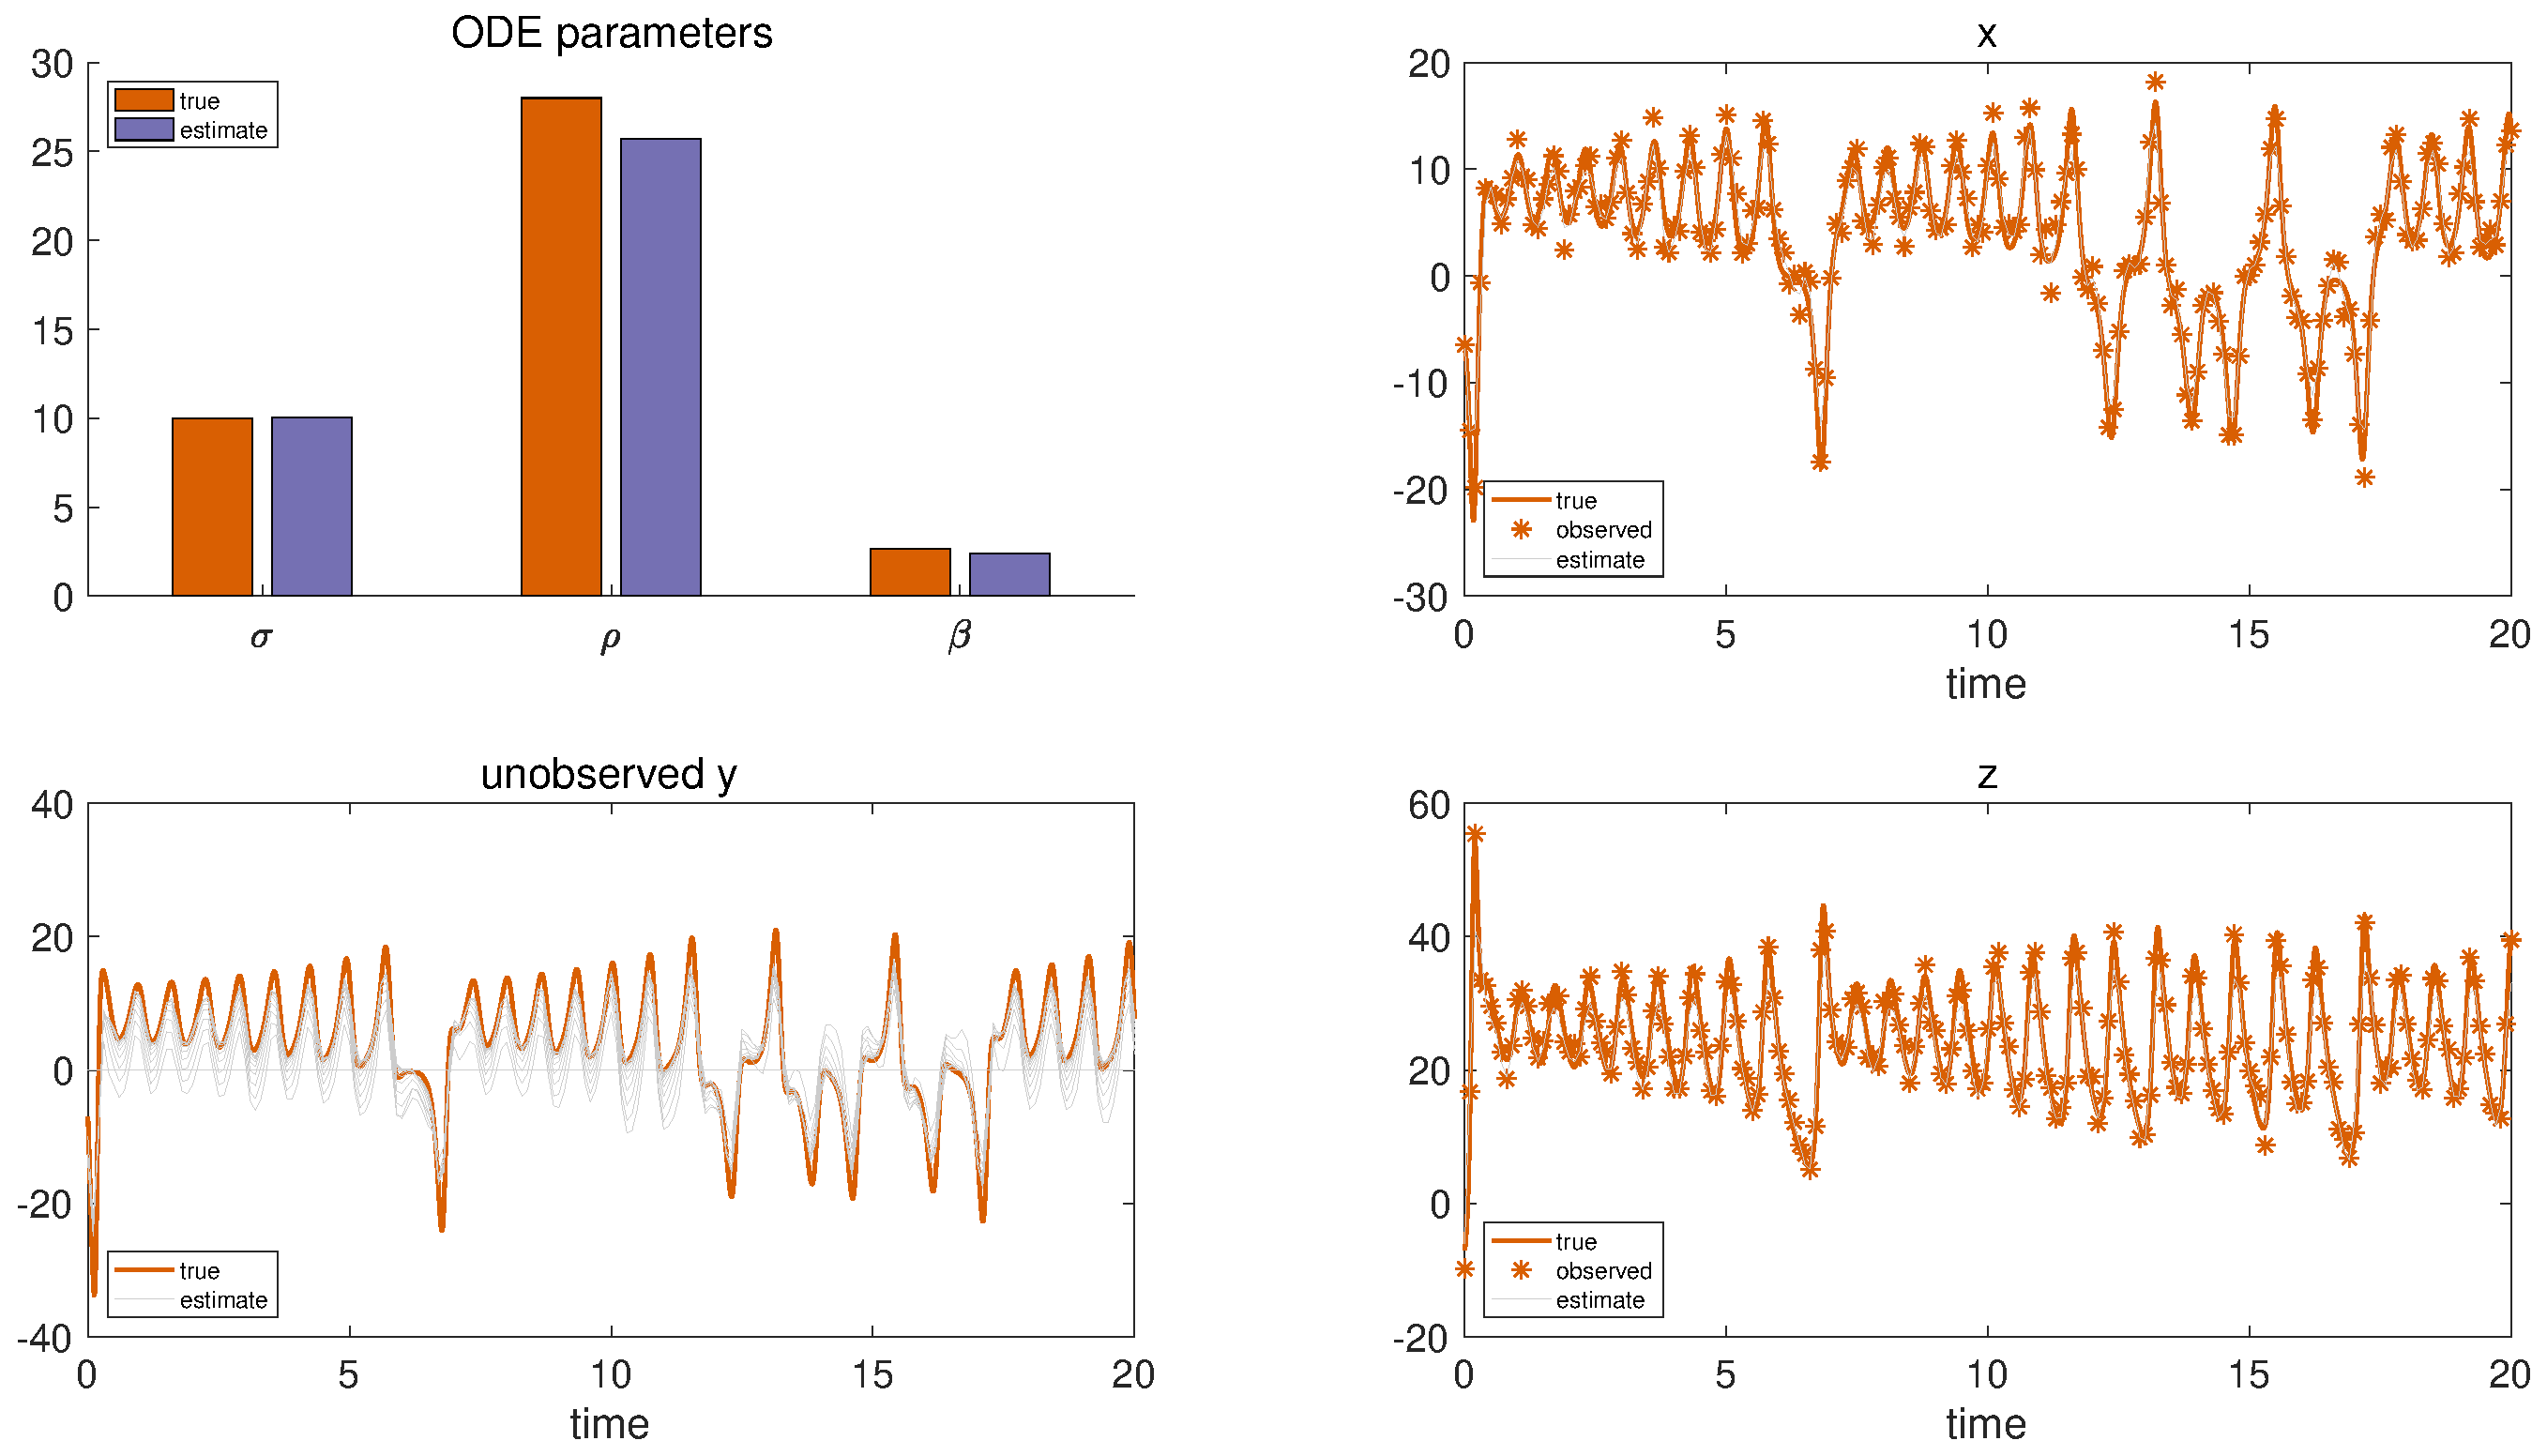
\includegraphics [width=4in]{Lorenz_attractor_4_38.eps}

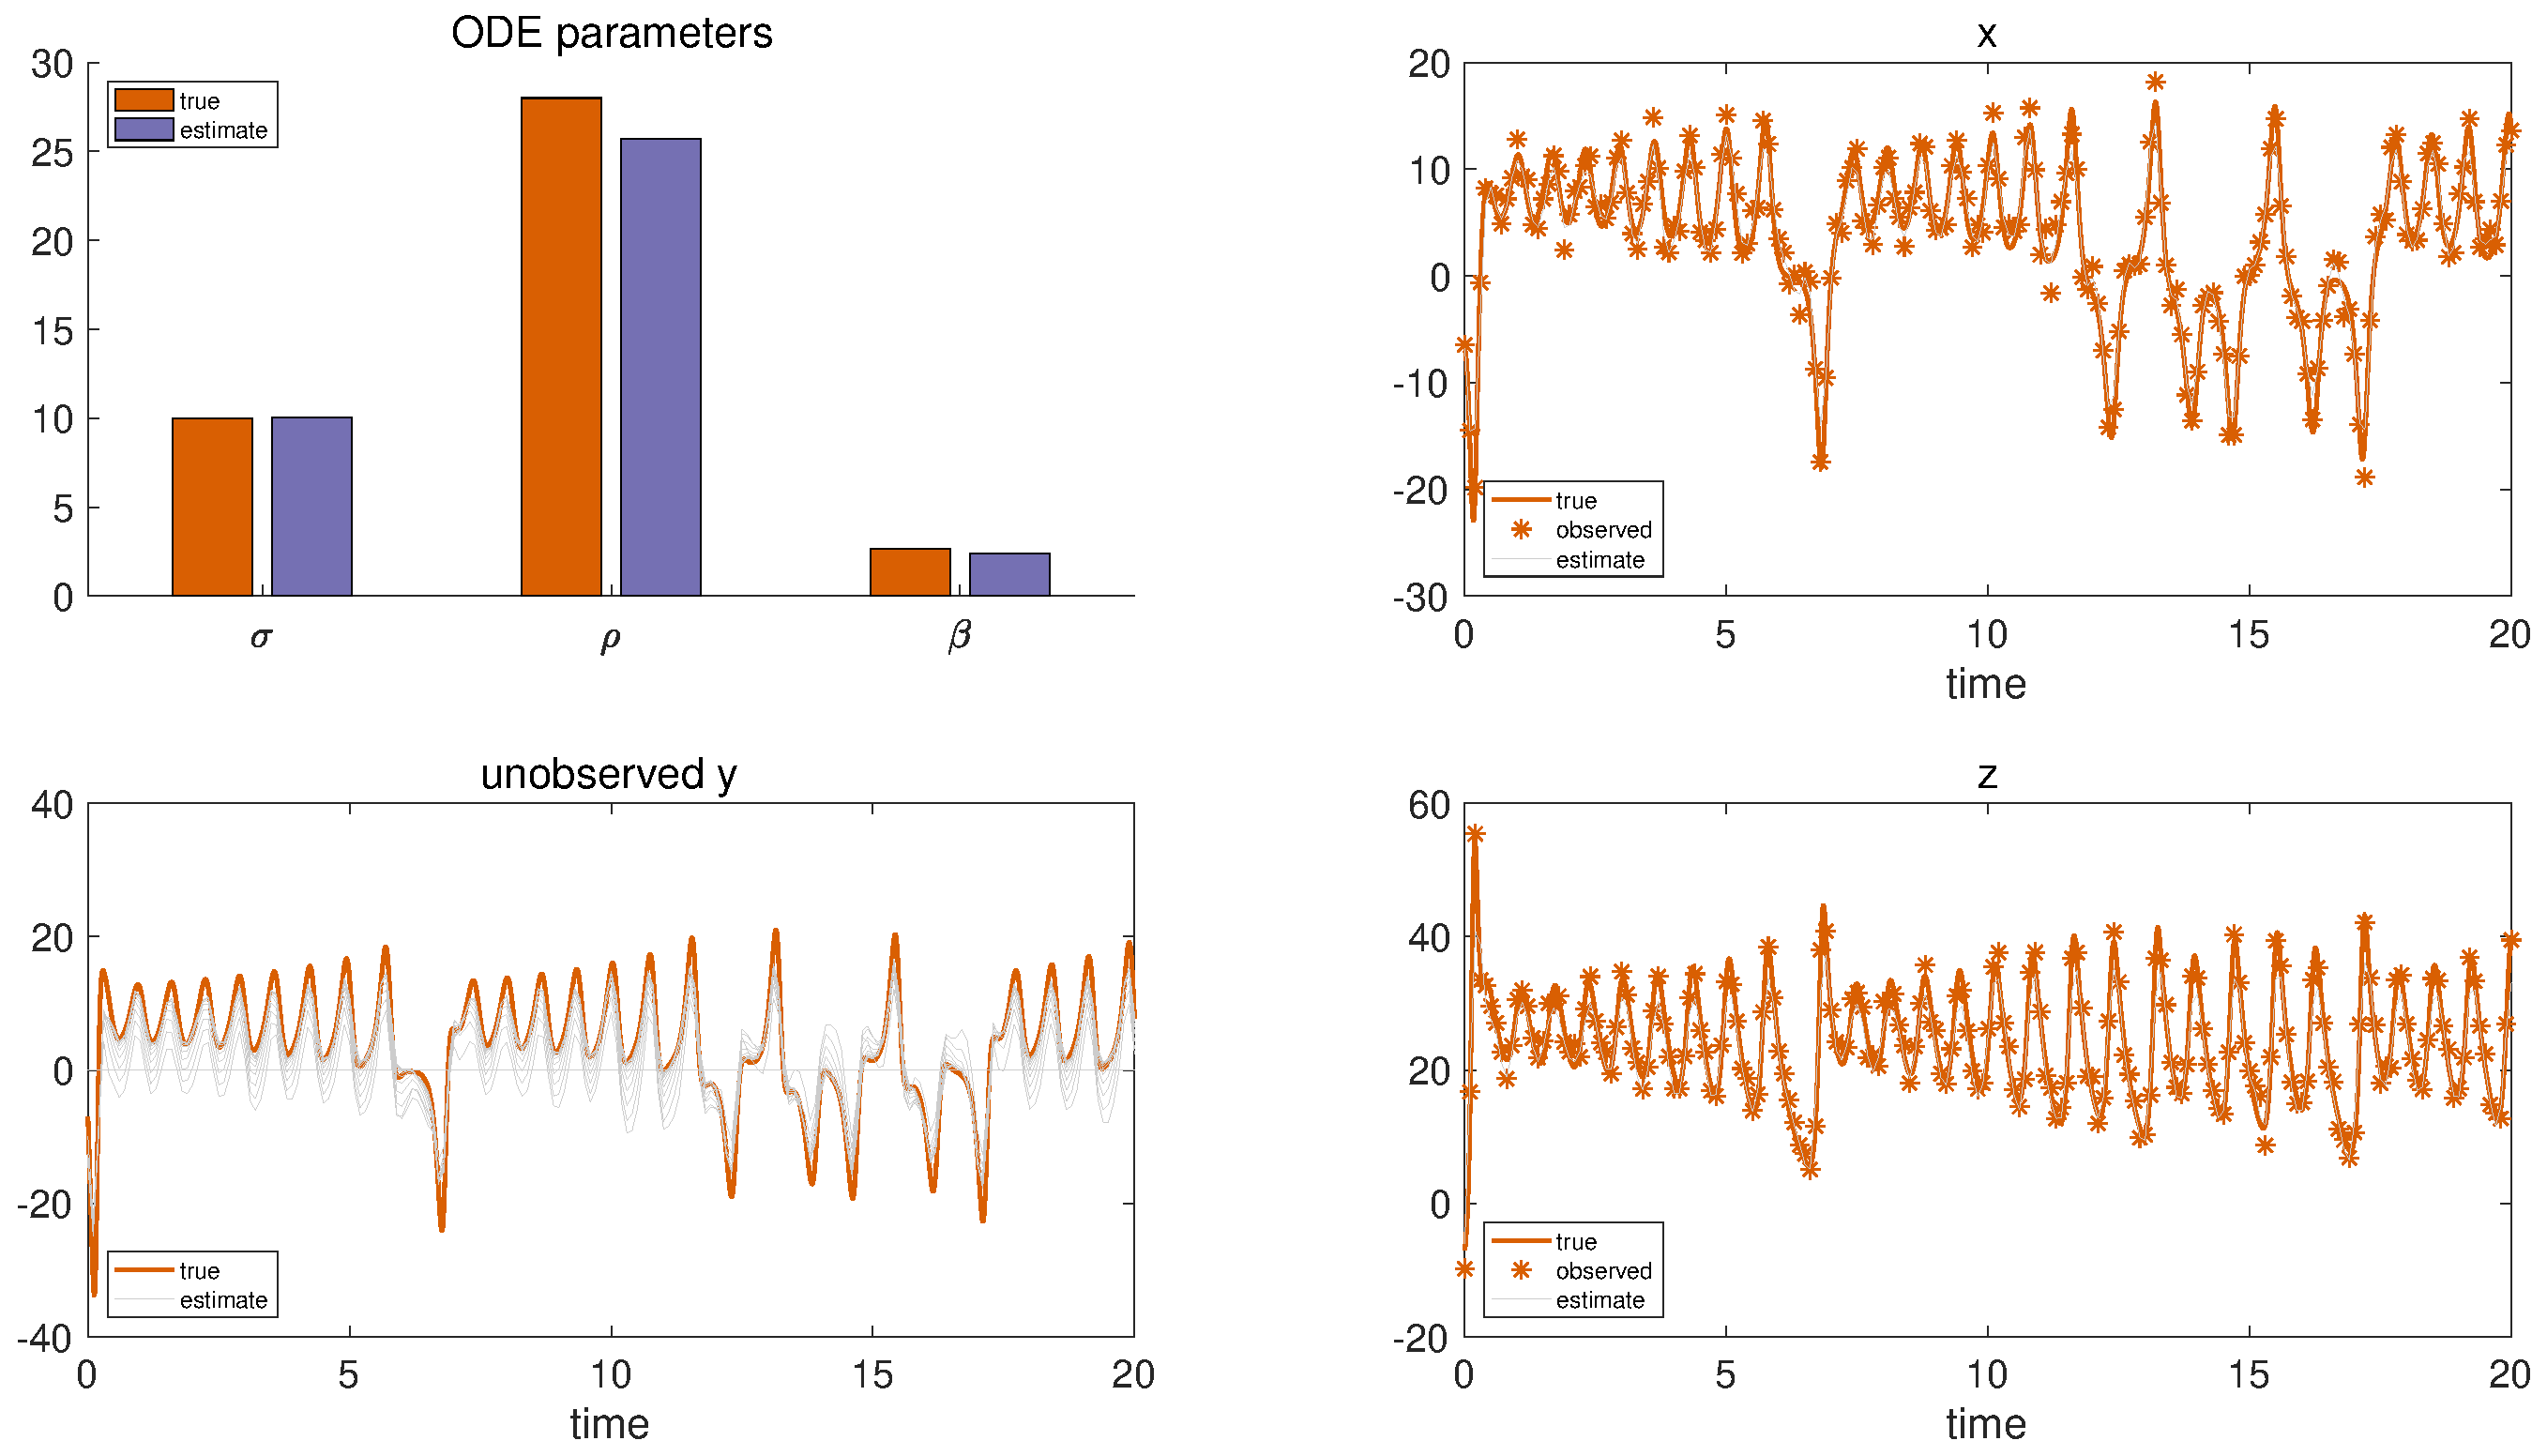
\includegraphics [width=4in]{Lorenz_attractor_4_39.eps}

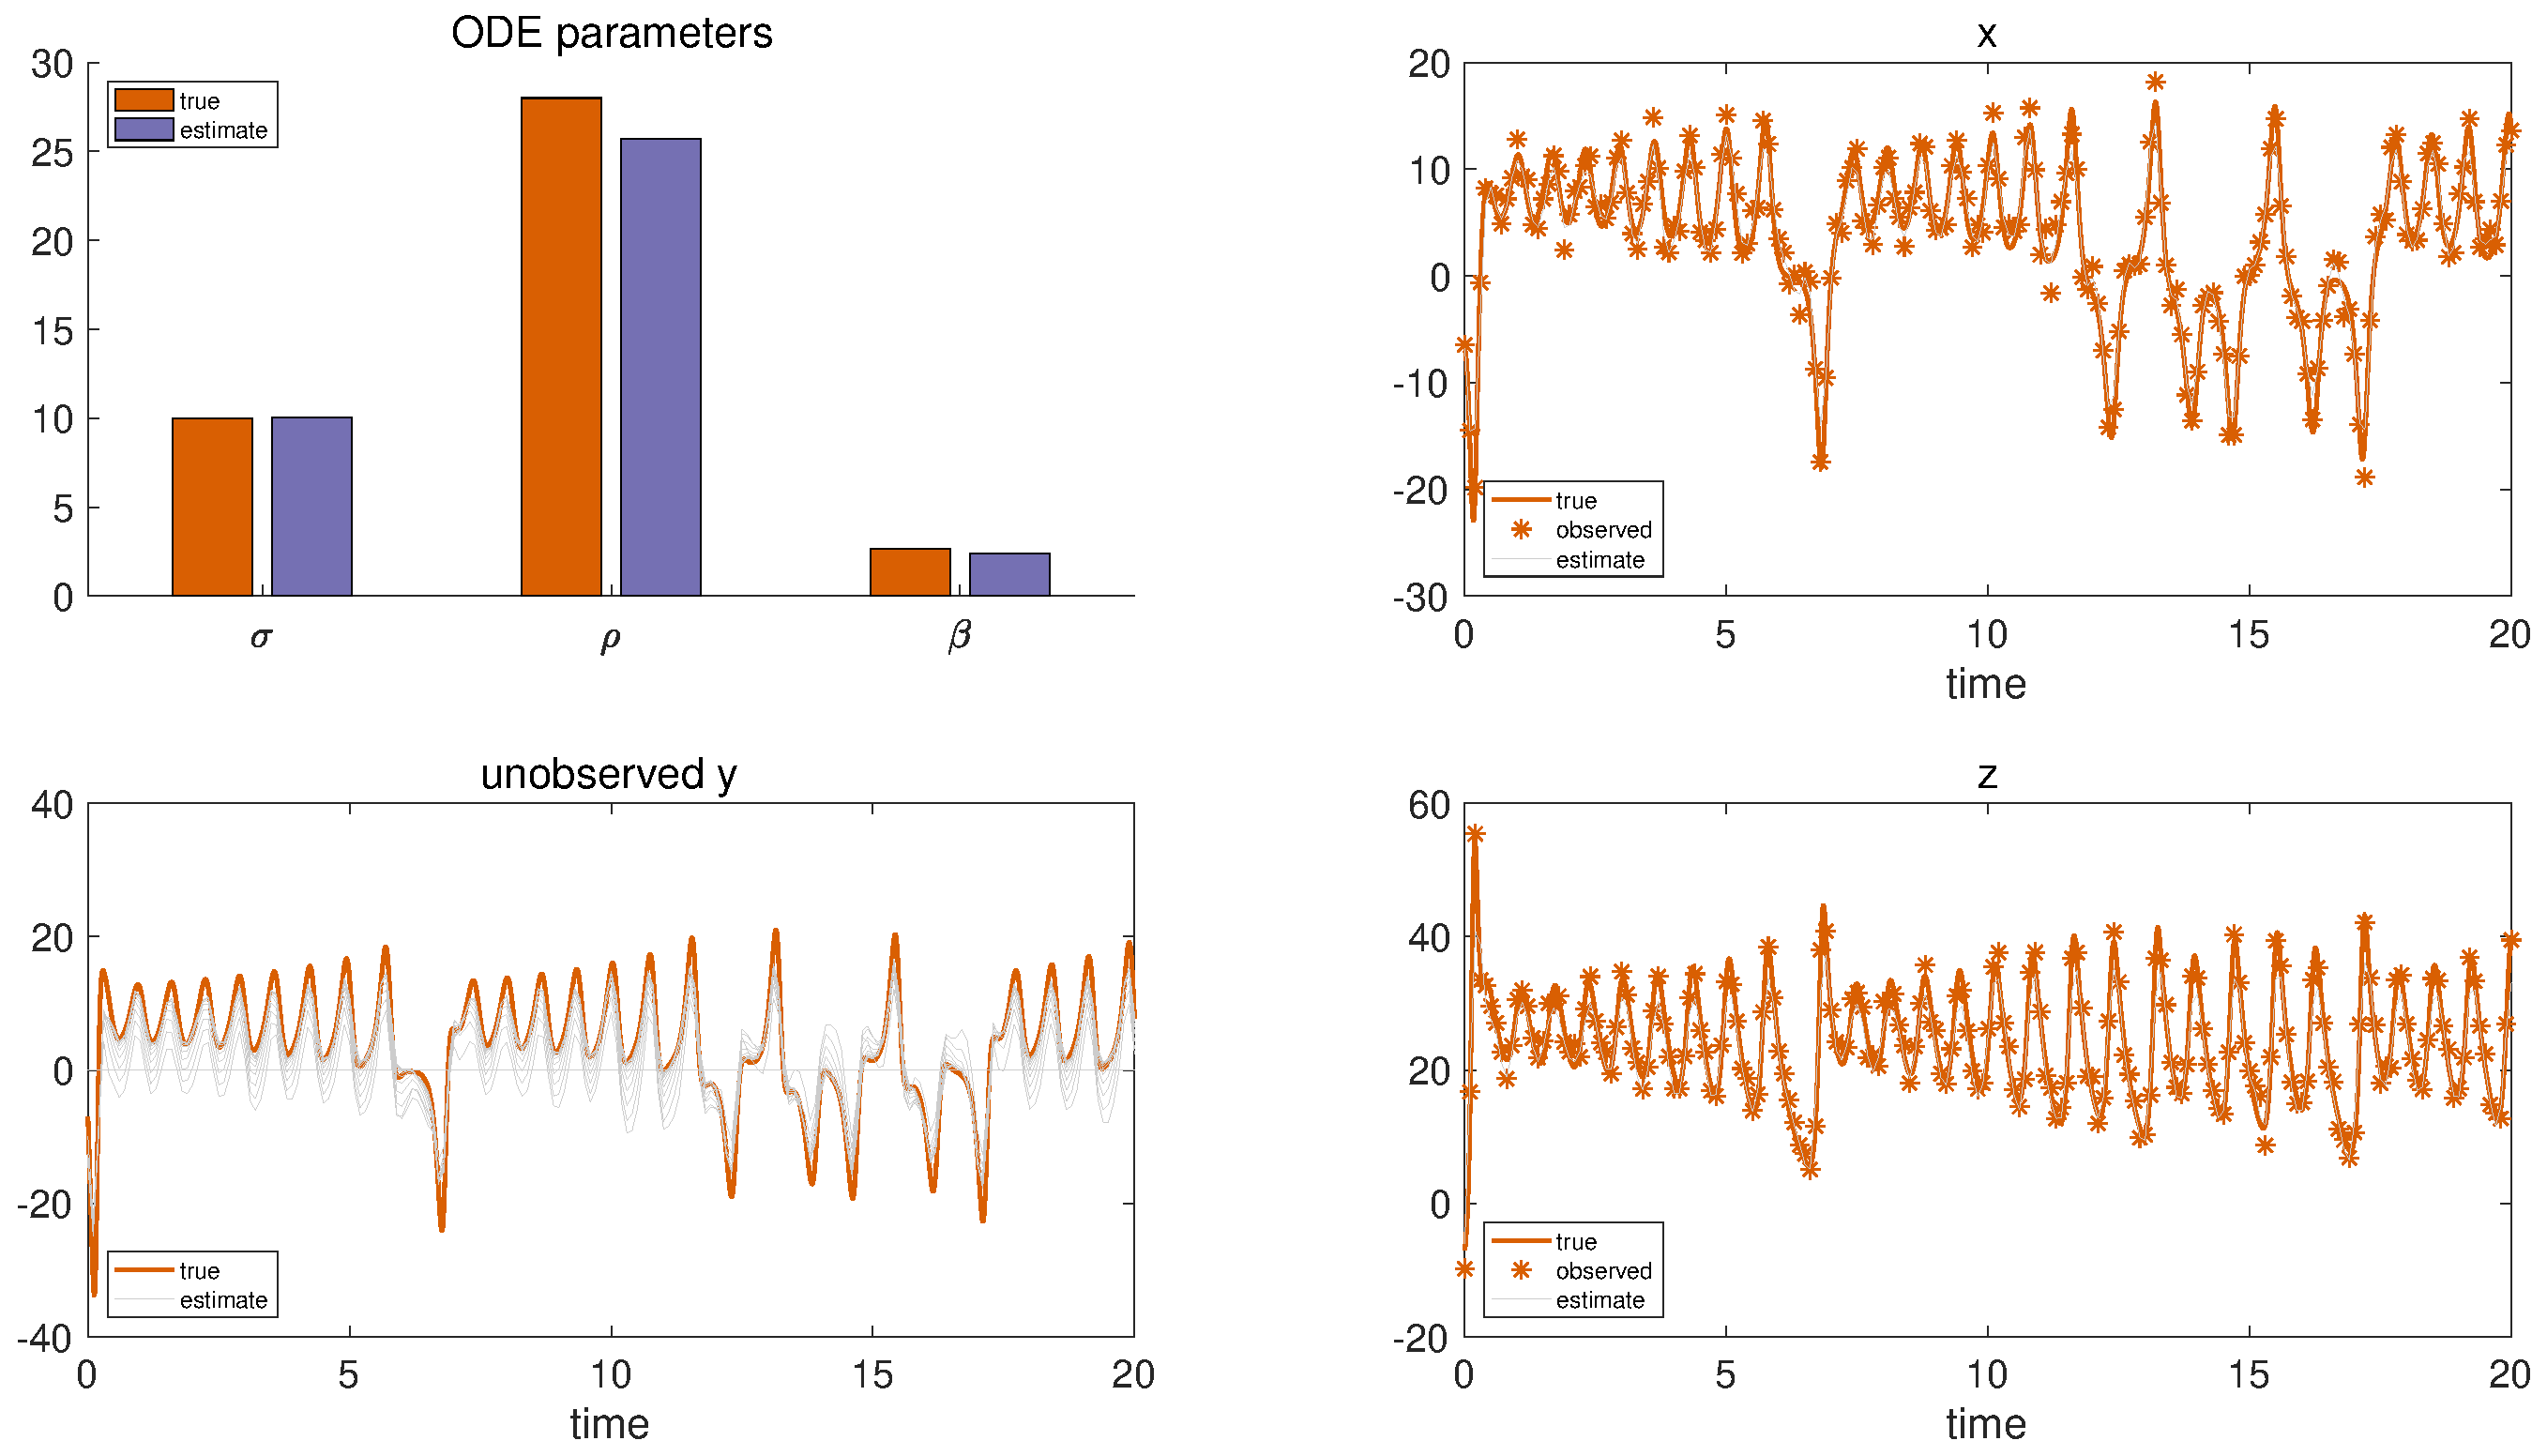
\includegraphics [width=4in]{Lorenz_attractor_4_40.eps}

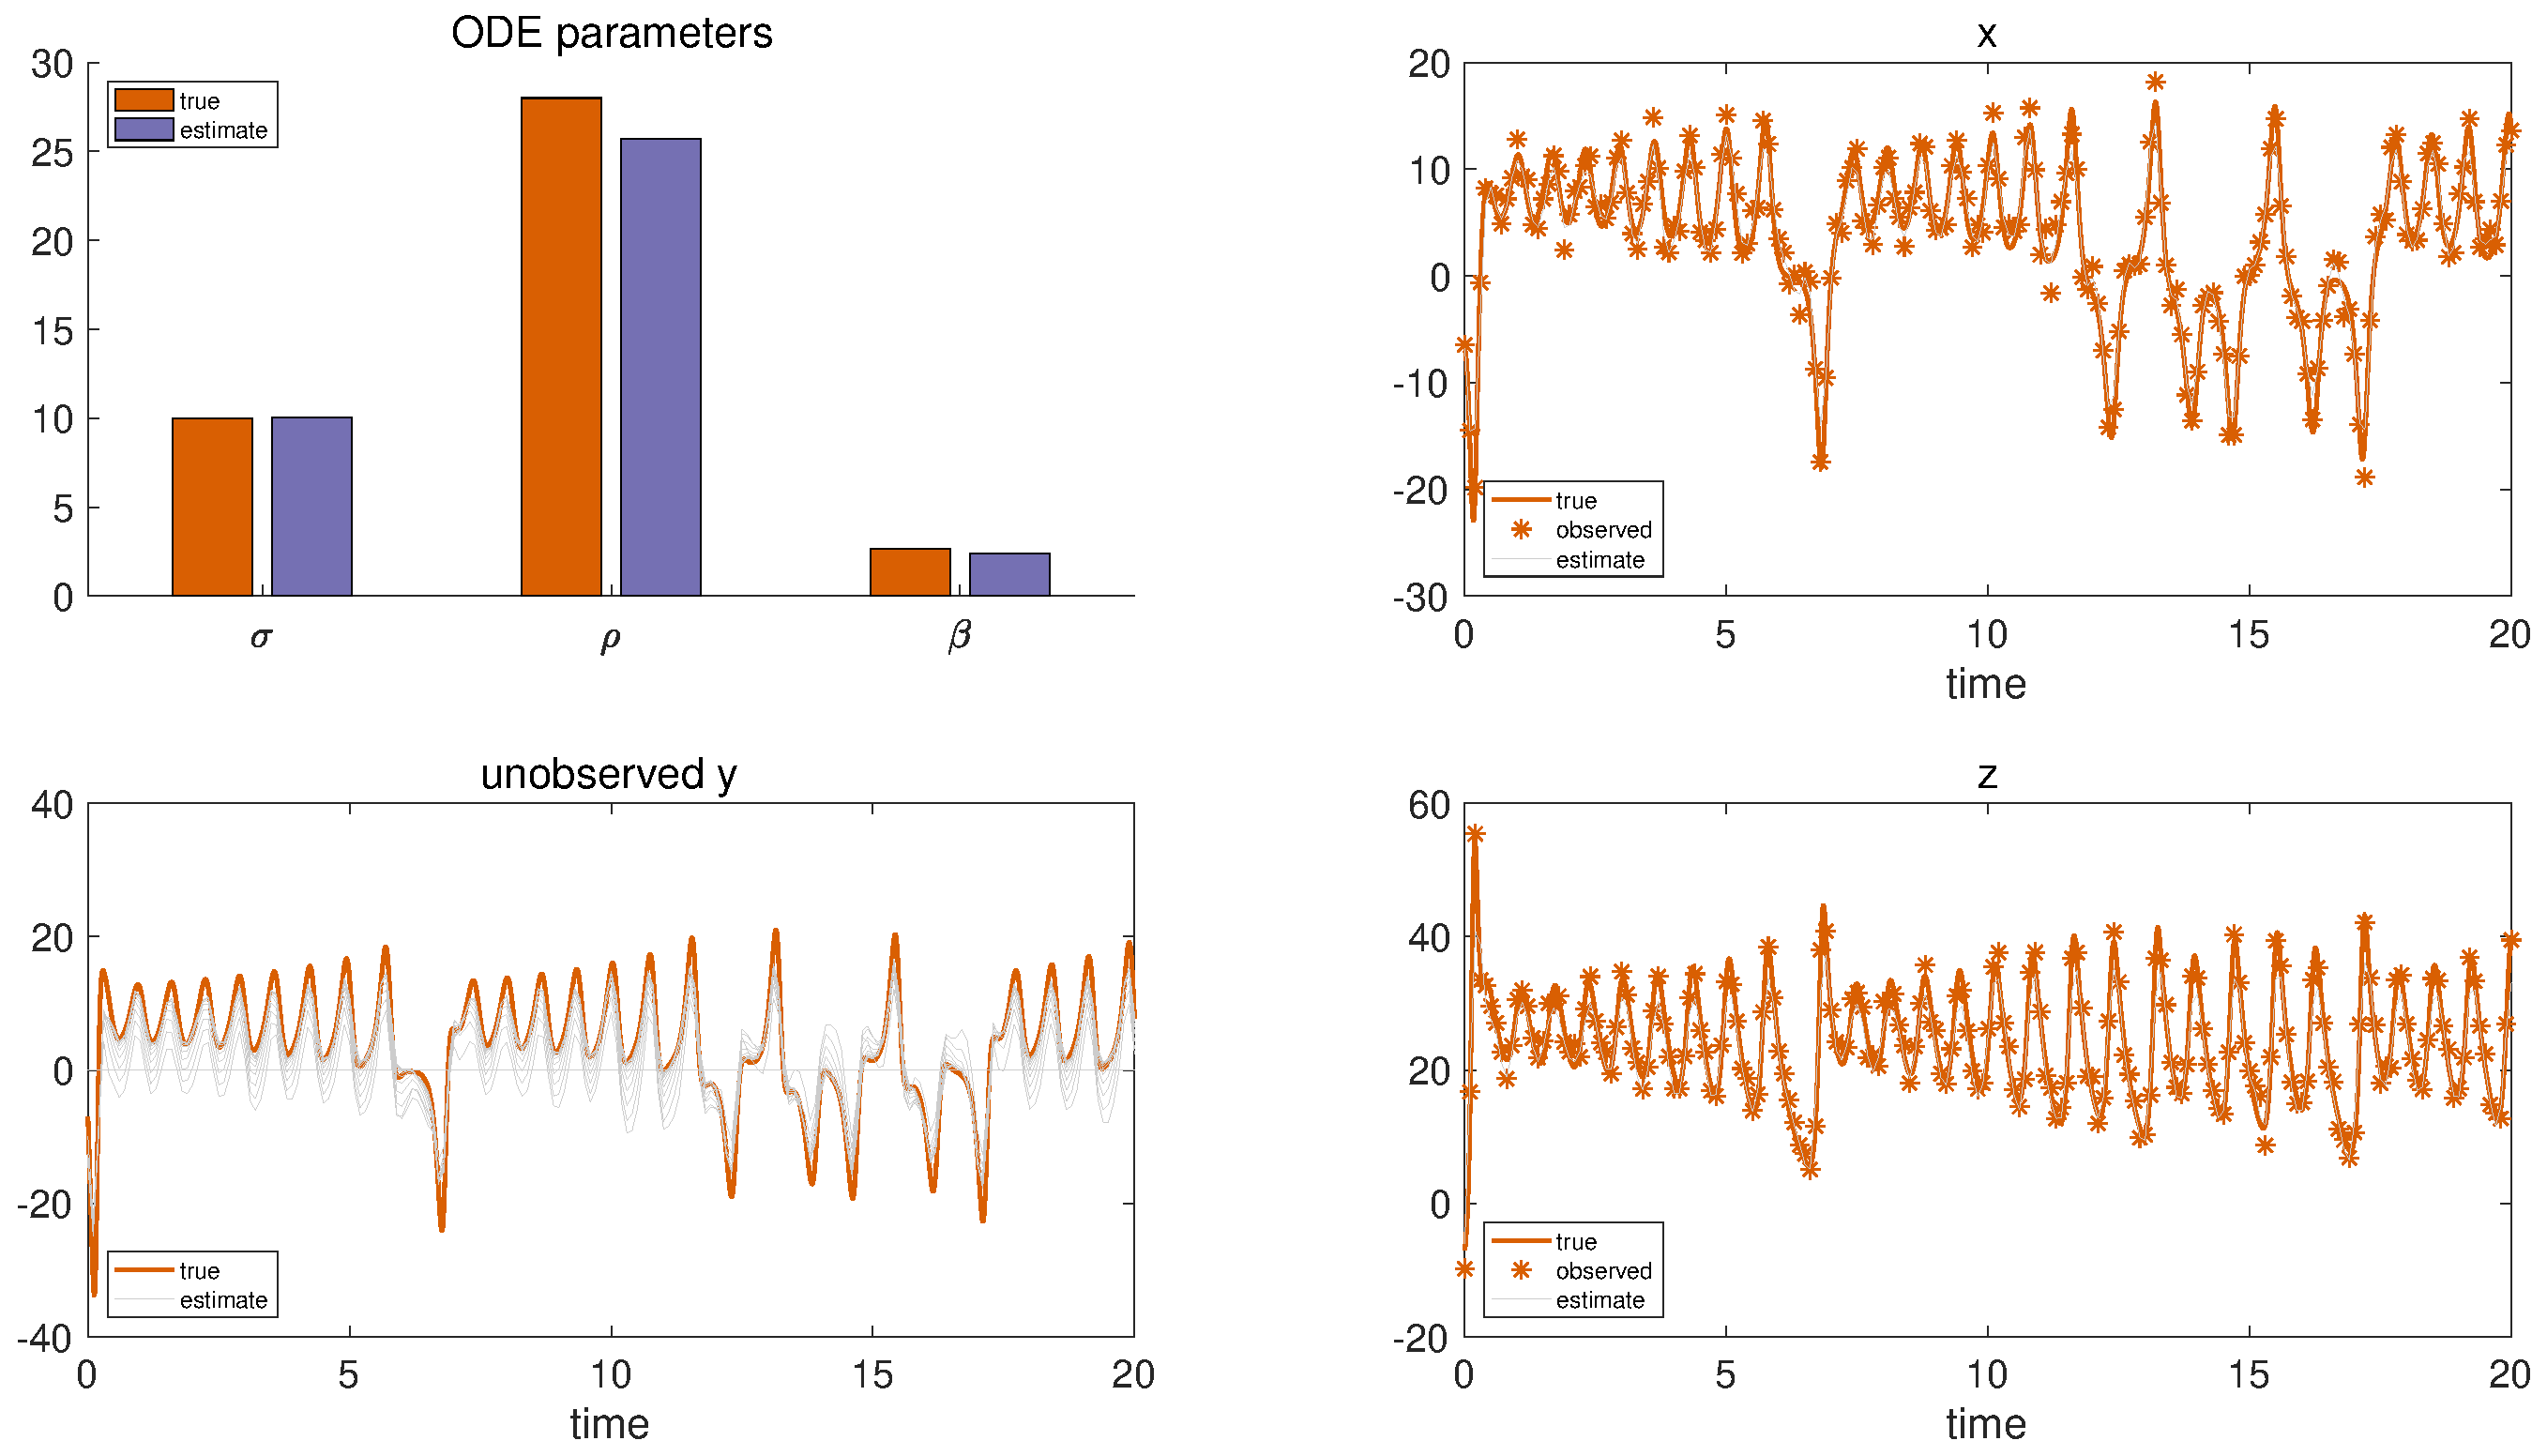
\includegraphics [width=4in]{Lorenz_attractor_4_41.eps}

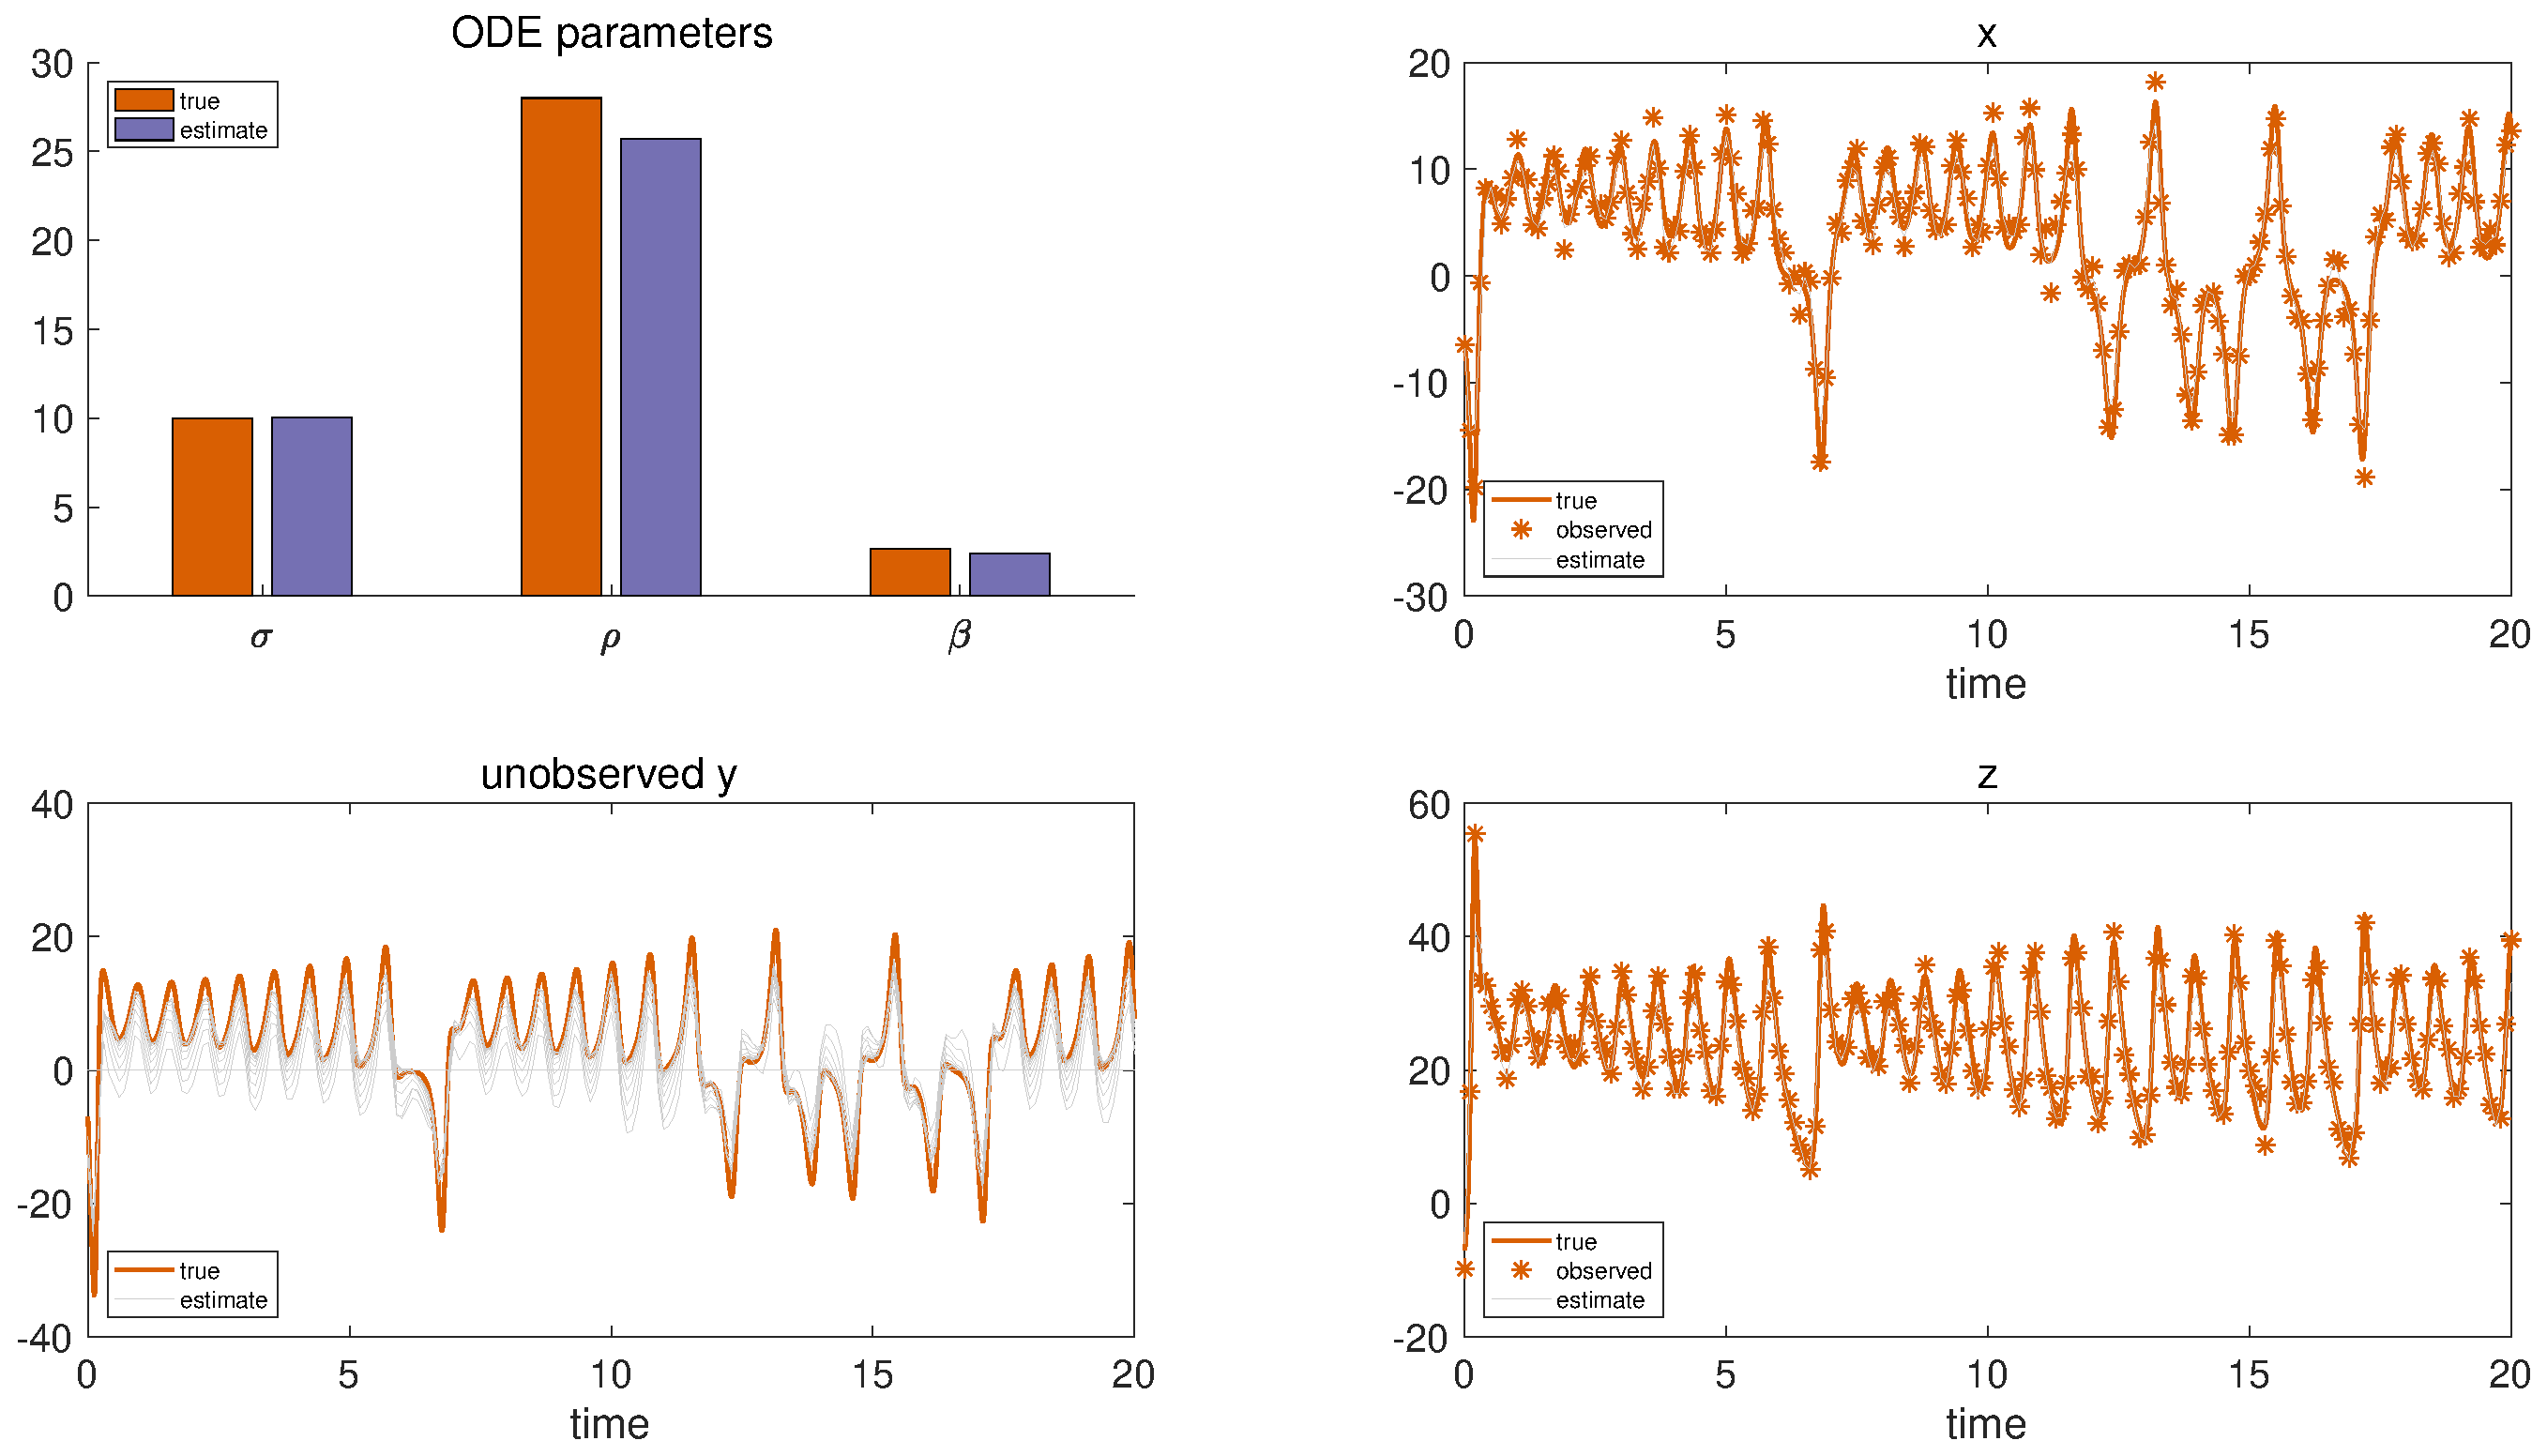
\includegraphics [width=4in]{Lorenz_attractor_4_42.eps}

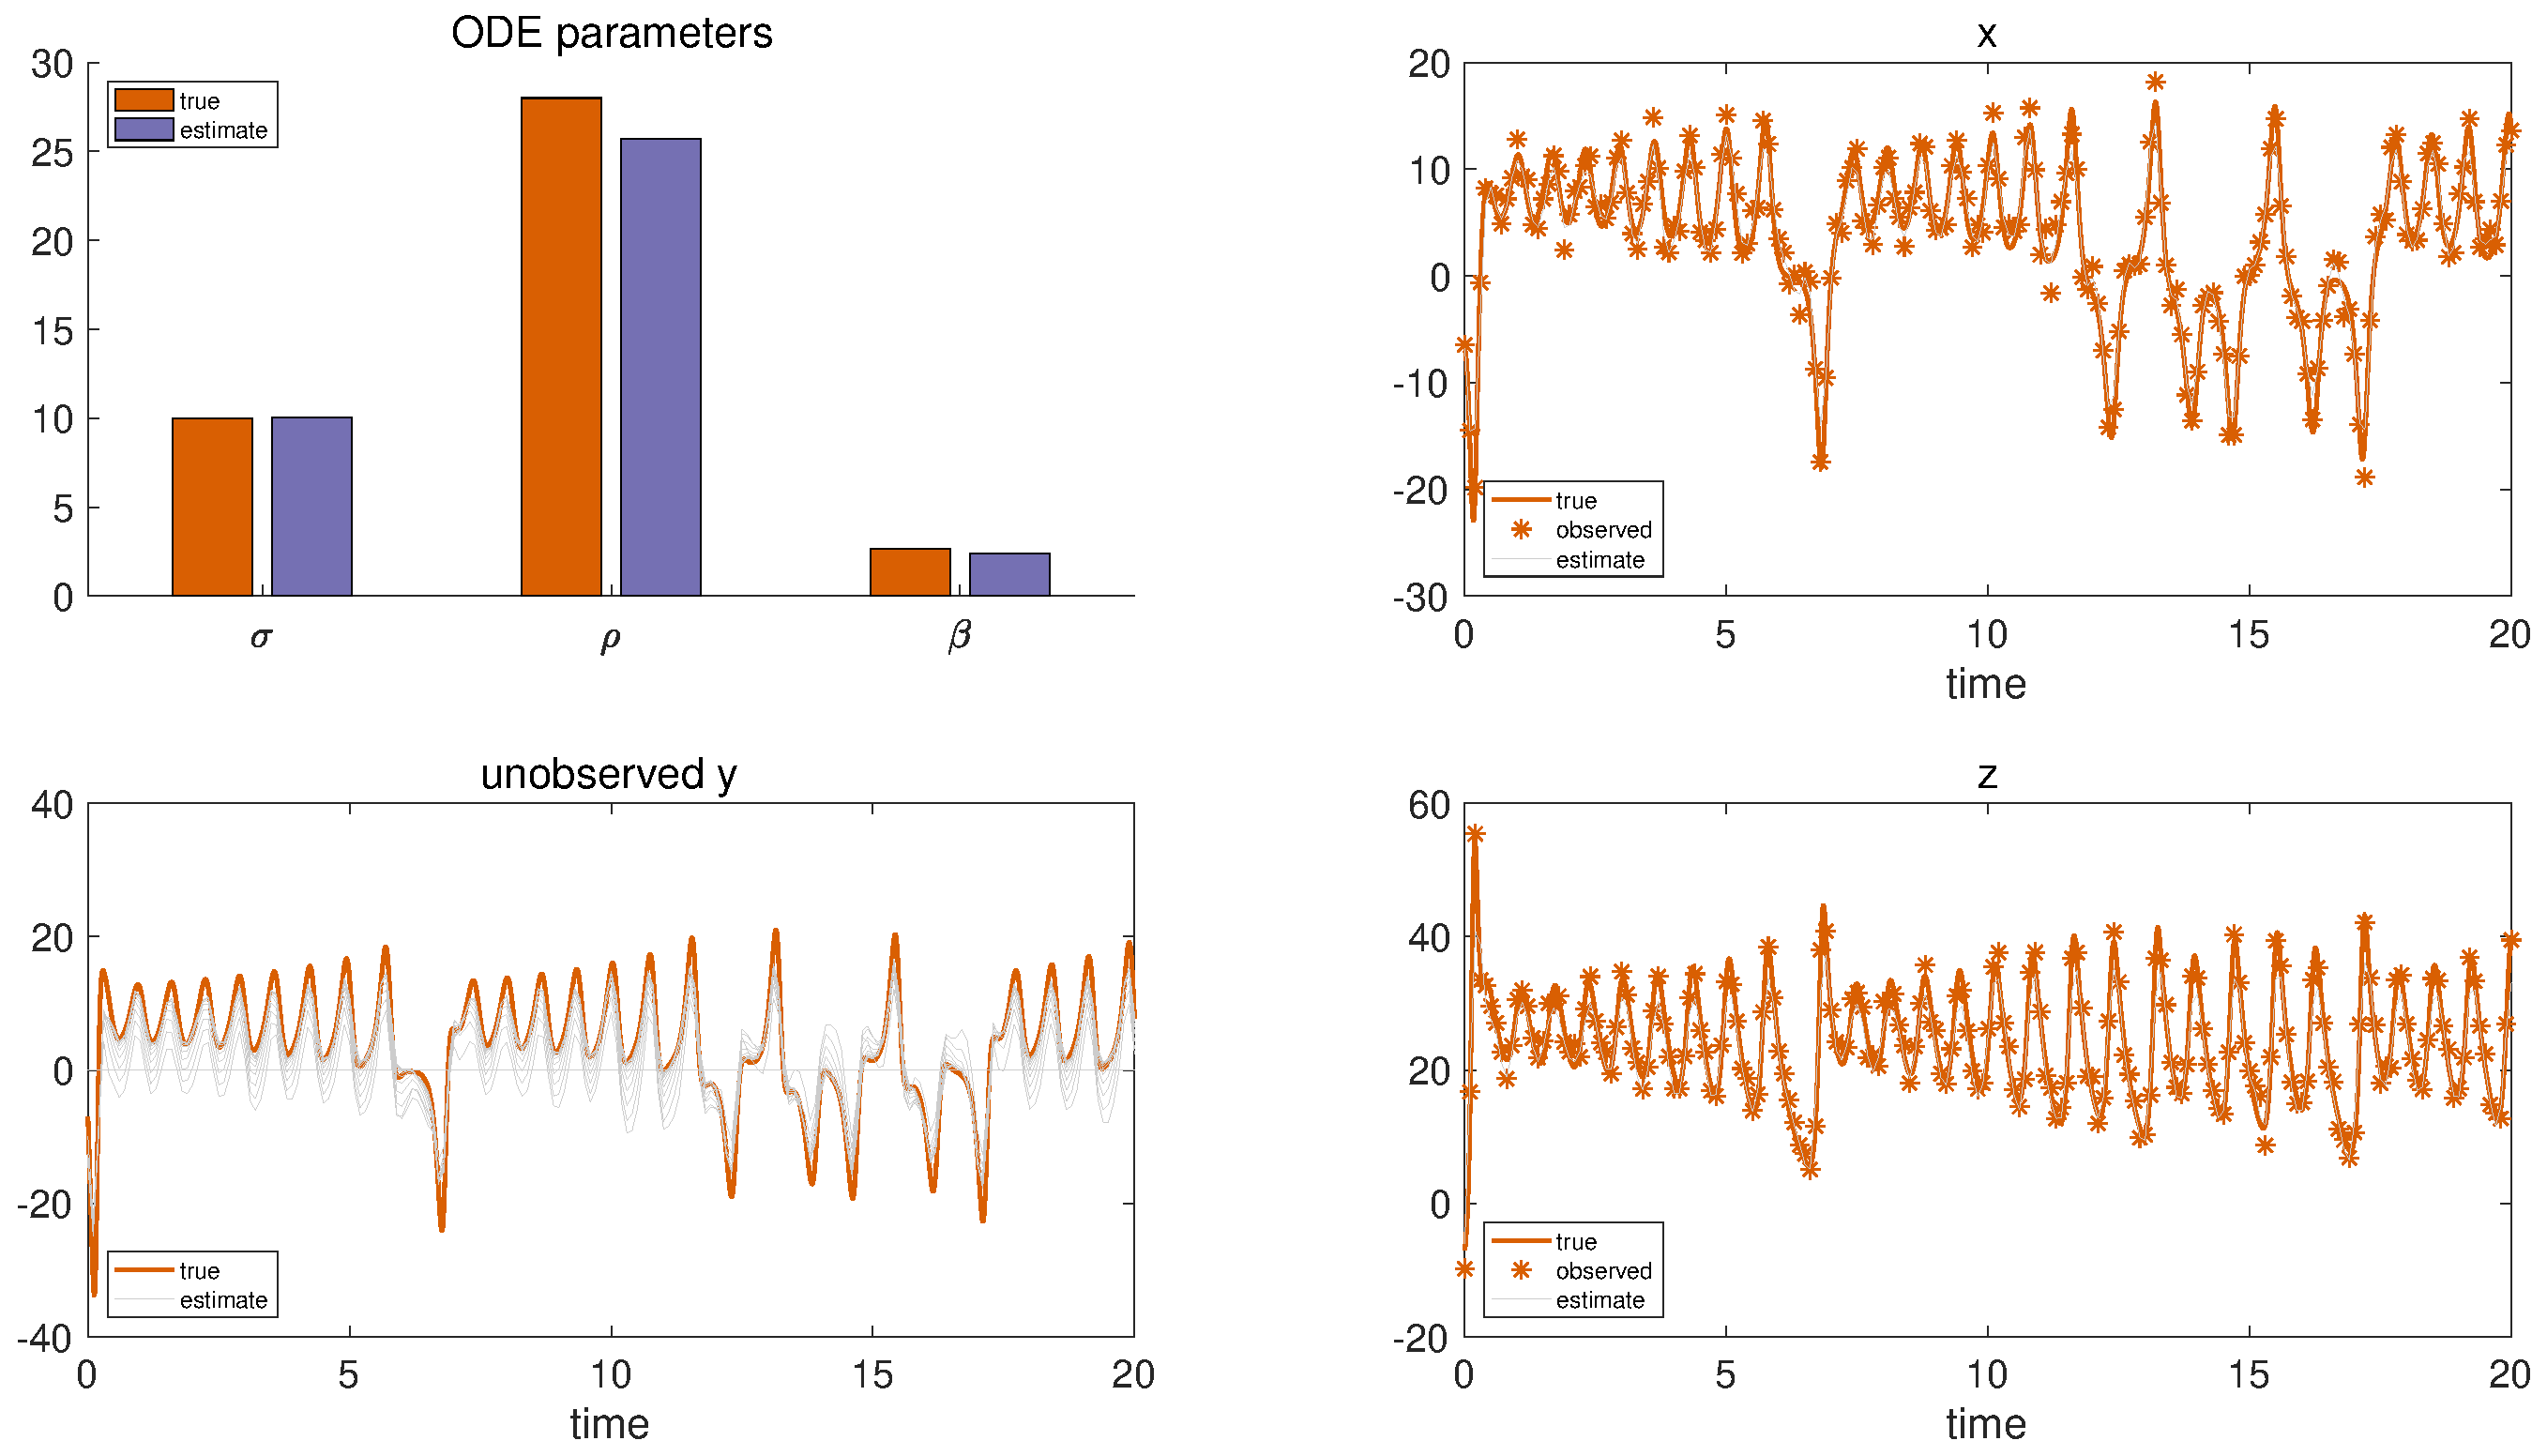
\includegraphics [width=4in]{Lorenz_attractor_4_43.eps}

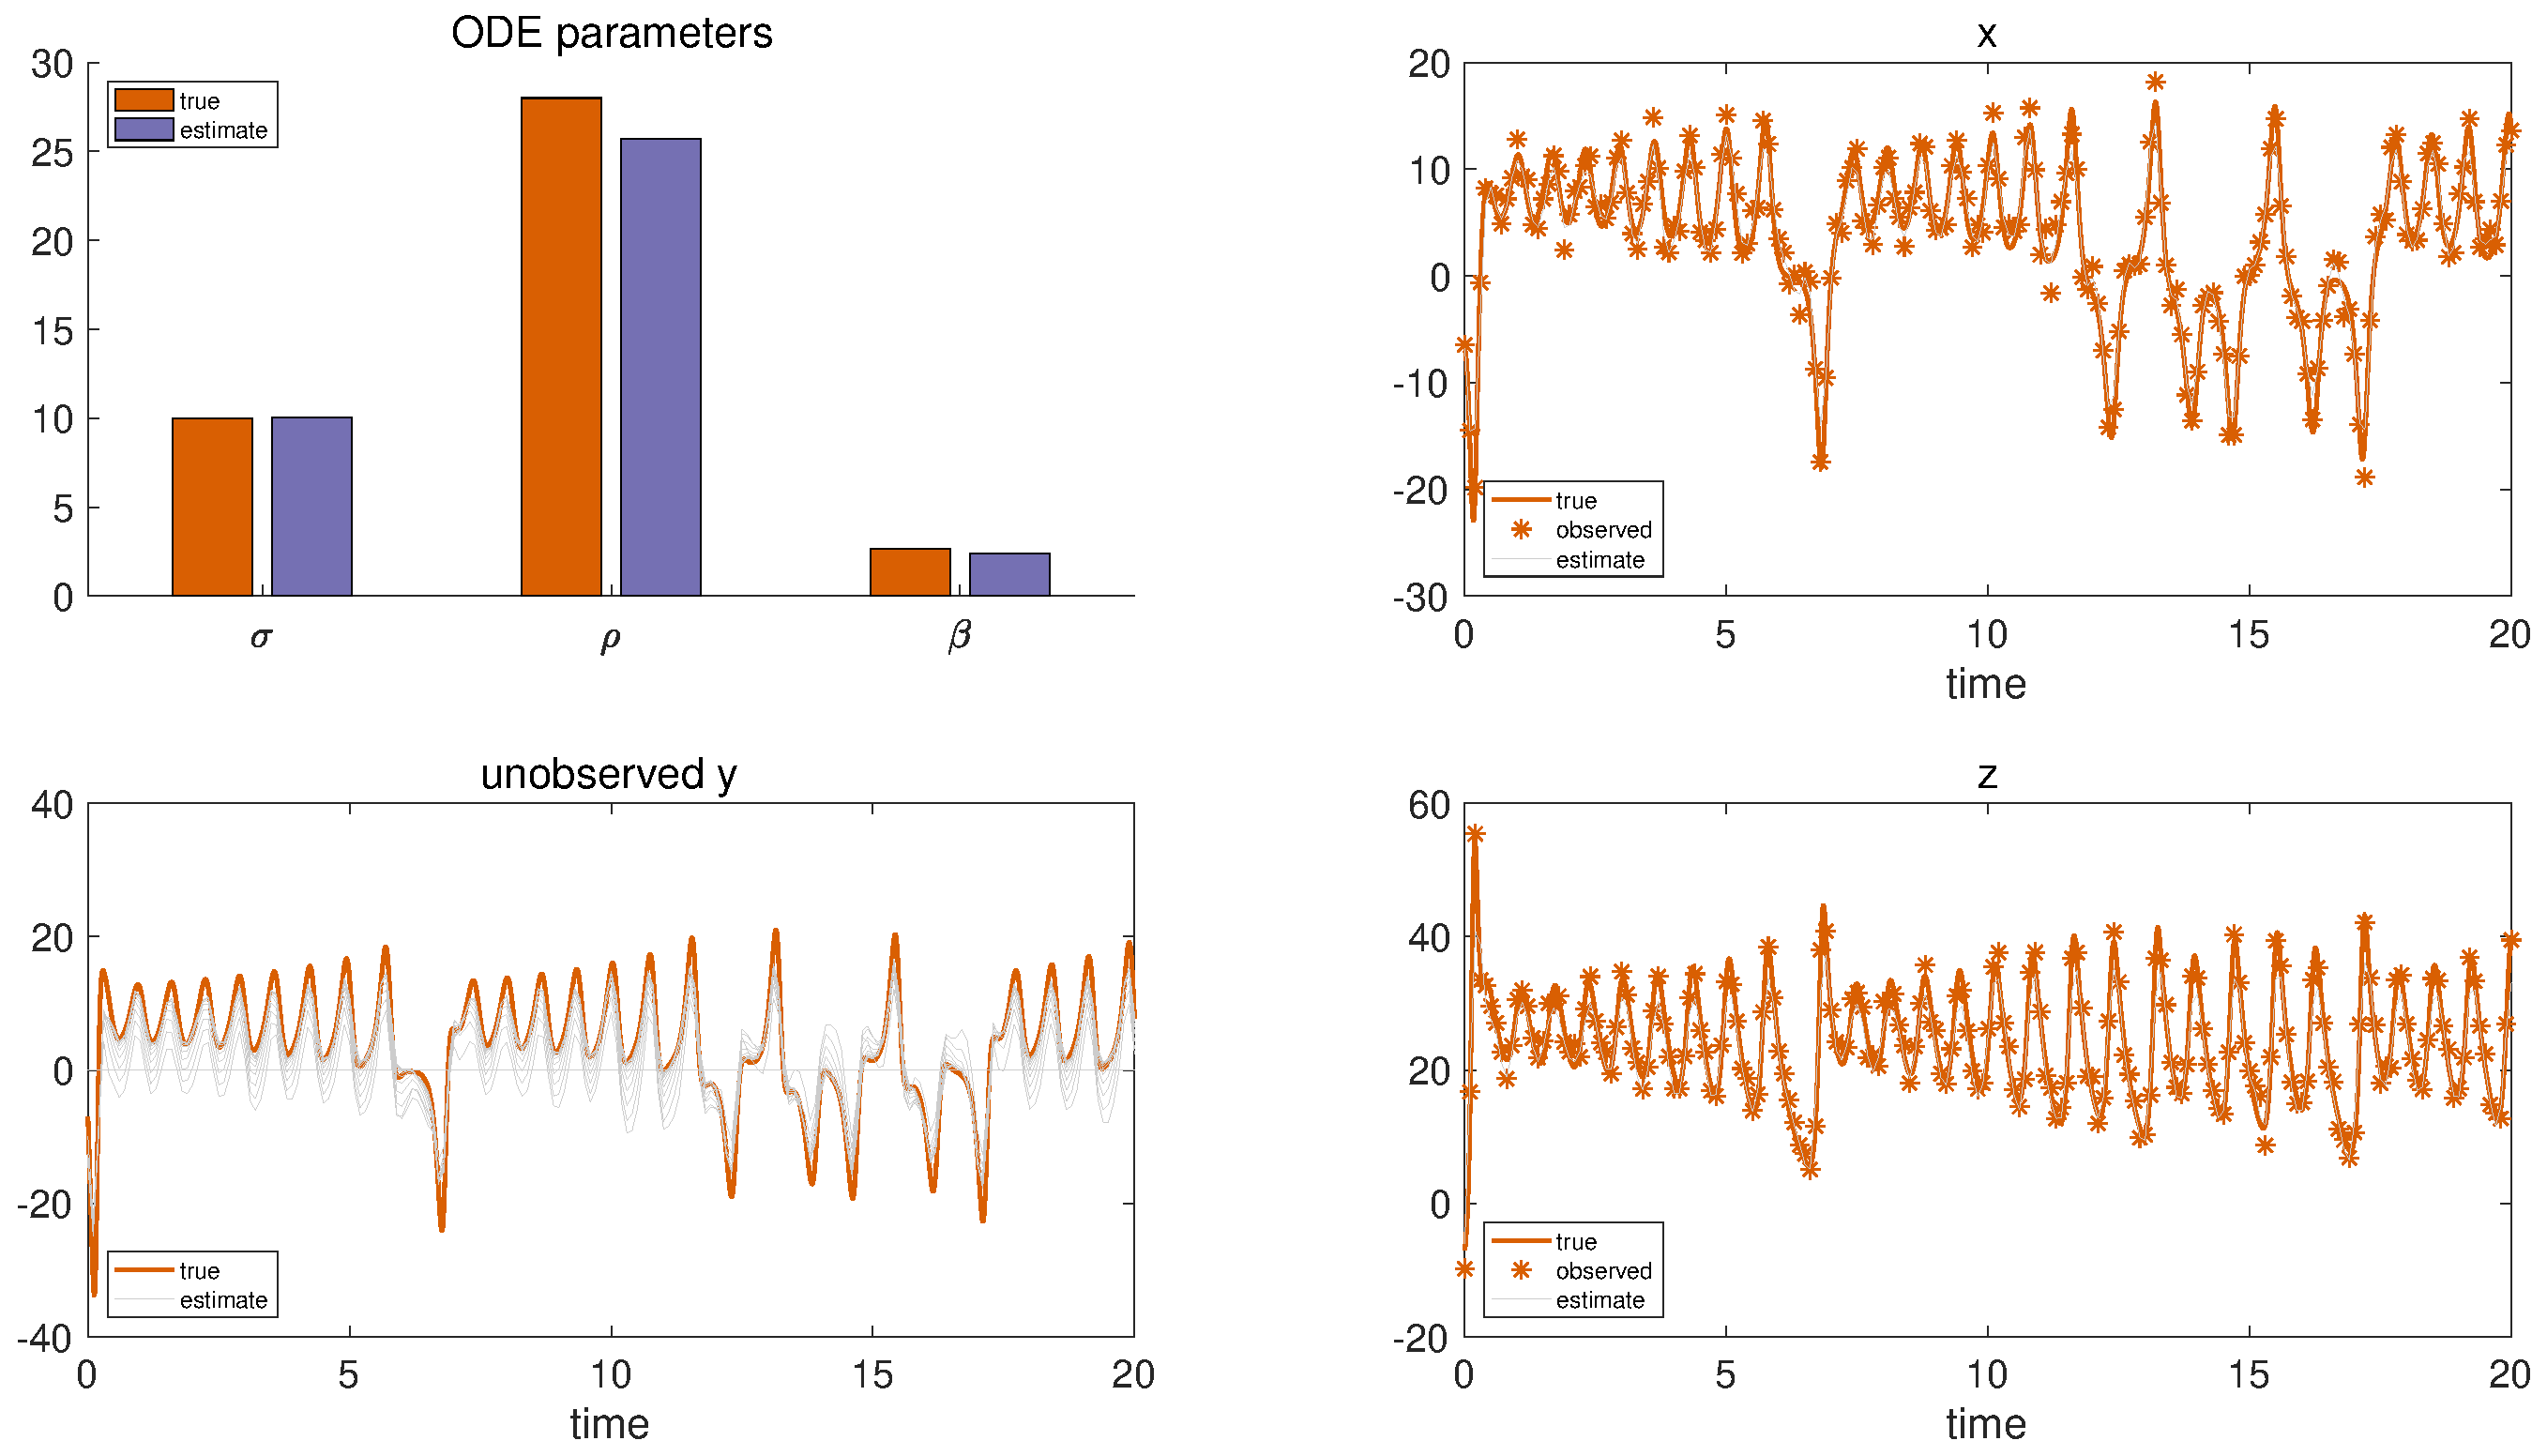
\includegraphics [width=4in]{Lorenz_attractor_4_44.eps}
\begin{par}
\ensuremath{\backslash}subsection\{ Proxy for individual states \}
\end{par} \vspace{1em}
\begin{par}
Expanding the proxy distribution in equation (12) over the individual state $\mathbf{x}_u$:
\end{par} \vspace{1em}
\begin{par}
$\hat{q}(\mathbf{x}_u) \stackrel{(a)}{\propto} \exp \left( ~ E_{Q_{-u}}  \ln ( p(\mathbf{x}_u \mid \theta, \mathbf{X}_{-u},\phi,\gamma) p(\mathbf{x}_u \mid\mathbf{Y},\phi,\sigma) ) ~ \right)$
\end{par} \vspace{1em}
\begin{par}
$\stackrel{(b)}{\propto} \exp\big( ~ E_{Q_{-u}} \ln \mathcal{N}\left(\mathbf{x}_u ; -\mathbf{B}_{u}^+ \mathbf{b}_u, ~\mathbf{B}_u^{+} ~ (\mathbf{A} + \mathbf{I}\gamma) ~ \mathbf{B}_u^{+T} \right) + E_{Q_{-u}} \ln \mathcal{N}\left(\mathbf{x}_u ; \boldmath\mu_u(\mathbf{Y}), \Sigma_u \right) \big)$
\end{par} \vspace{1em}
\begin{par}
$= \exp\big( ~ E_{Q_{-u}} \ln \mathcal{N}\left(\mathbf{x}_u ; \left( \mathbf{B}_{u} \mathbf{B}_{u}^T \right)^{-1} \left( - \sum_k \mathbf{B}_{uk}^T \mathbf{b}_{uk} \right), ~\mathbf{B}_{u}^{+} ~ (\mathbf{A} + \mathbf{I}\gamma) ~ \mathbf{B}_u^{+T} \right) + E_{Q_{-u}} \ln \mathcal{N}\left(\mathbf{x}_u ; \boldmath\mu_u(\mathbf{Y}), \Sigma_u \right) \big)$,
\end{par} \vspace{1em}
\begin{par}
which, once more, can be normalized analytically due to its exponential quadratic form. In (a) we decompose the full conditional into an ODE-informed distribution and a data-informed distribution and in (b) we substitute the ODE-informed distribution $p(\mathbf{x}_u \mid \theta, \mathbf{X}_{-u},\phi,\gamma)$ with its density given by equation (8).
\end{par} \vspace{1em}
\begin{verbatim}
    [state.proxy.mean,state.proxy.inv_cov] = proxy_for_ind_states(state.lin_comb,...
        state.proxy.mean,param_proxy_mean',dC_times_invC,coupling_idx.states,symbols,...
        mu,inv_sigma,simulation.observed_states,A_plus_gamma_inv,opt_settings);
\end{verbatim}
\begin{verbatim}
end
\end{verbatim}
\begin{par}
\ensuremath{\backslash}subsection\{ Final result \}
\end{par} \vspace{1em}
\begin{verbatim}
plot_results(h_states,h_param,state,time,simulation,param_proxy_mean,p,symbols,'final');
\end{verbatim}

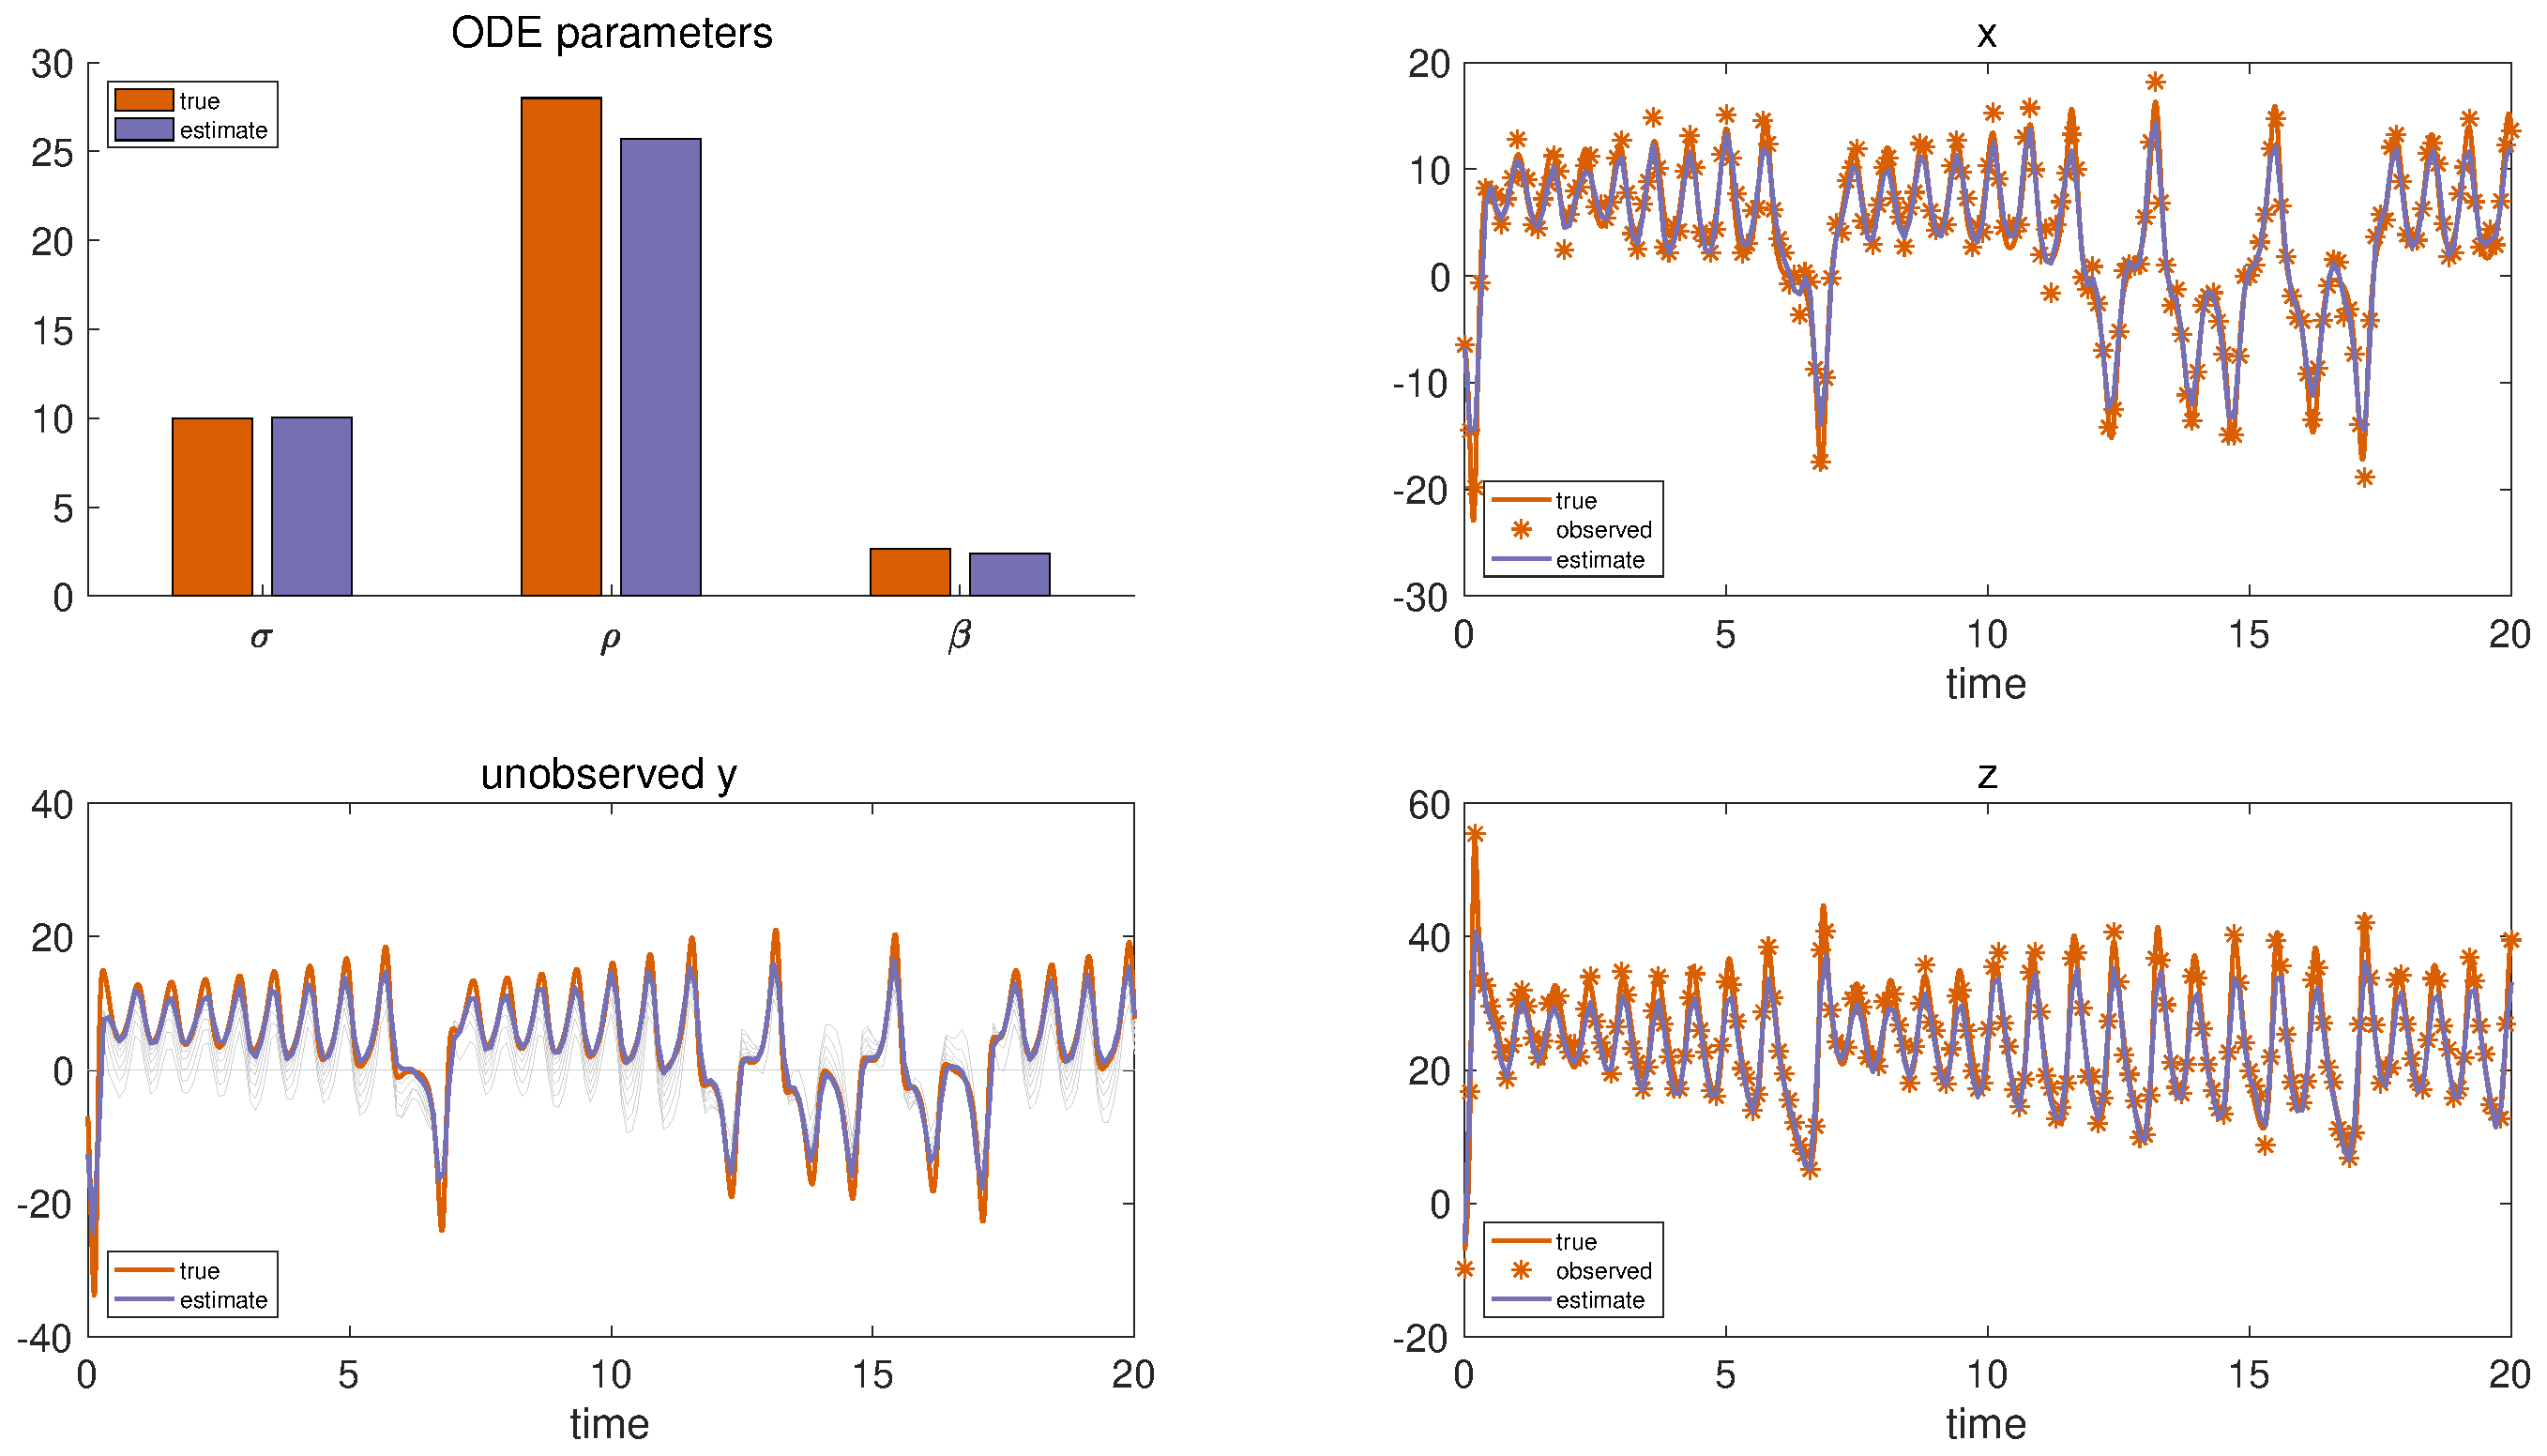
\includegraphics [width=4in]{Lorenz_attractor_4_45.eps}


\subsection*{Time Taken}

\begin{verbatim}
disp(['time taken: ' num2str(toc) ' seconds'])
\end{verbatim}

        \color{lightgray} \begin{verbatim}time taken: 71.0552 seconds
\end{verbatim} \color{black}
    

\subsection*{References}

\begin{itemize}
\setlength{\itemsep}{-1ex}
   \item \textbf{Gorbach, N.S.} , \textbf{Bauer, S.} and Buhmann, J.M., Scalable Variational Inference for Dynamical Systems. 2017a. Neural Information Processing Systems (NIPS). \begin{verbatim}https://papers.nips.cc/paper/7066-scalable-variational-inference-for-dynamical-systems.pdf\end{verbatim}, arxiv: \begin{verbatim}https://arxiv.org/abs/1705.07079\end{verbatim}.
   \item \textbf{Bauer, S.} , \textbf{Gorbach, N.S.} and Buhmann, J.M., Efficient and Flexible Inference for Stochastic Differential Equations. 2017b. Neural Information Processing Systems (NIPS). \begin{verbatim}https://papers.nips.cc/paper/7274-efficient-and-flexible-inference-for-stochastic-systems.pdf\end{verbatim}
   \item Wenk, P., Gotovos, A., Bauer, S., Gorbach, N.S., Krause, A. and Buhmann, J.M., Fast Gaussian Process Based Gradient Matching for Parameters Identification in Systems of Nonlinear ODEs. 2018. In submission to Conference on Uncertainty in Artificial Intelligence (UAI).
   \item Calderhead, B., Girolami, M. and Lawrence. N.D., 2002. Accelerating Bayesian inference over nonlinear differential equation models. \textit{In Advances in Neural Information Processing Systems (NIPS)} . 22.
\end{itemize}
\begin{par}
The authors in bold font have contributed equally to their respective papers.
\end{par} \vspace{1em}


\subsection*{Subroutines}

\begin{par}
\ensuremath{\backslash}subsection\{ Kernel function \}
\end{par} \vspace{1em}
\begin{par}
Gradient matching with Gaussian processes assumes a joint Gaussian process prior on states and their derivatives:
\end{par} \vspace{1em}
\begin{par}
$\left(\begin{array}{c} \mathbf{X} \\ \dot{\mathbf{X}} \end{array}\right)  \sim \mathcal{N} \left( \begin{array}{c} \mathbf{X} \\ \dot{\mathbf{X}} \end{array}; \begin{array}{c}  \mathbf{0} \\ \mathbf{0}  \end{array}, \begin{array}{cc}  \mathbf{C}_{\phi} & \mathbf{C}_{\phi}' \\ '\mathbf{C}_{\phi} &  \mathbf{C}_{\phi}'' \end{array} \right)$,
\end{par} \vspace{1em}
\begin{par}
$\mathrm{cov}(x_k(t), x_k(t)) = C_{\phi_k}(t,t')$
\end{par} \vspace{1em}
\begin{par}
$\mathrm{cov}(\dot{x}_k(t), x_k(t)) = \frac{\partial C_{\phi_k}(t,t') }{\partial t} =: C_{\phi_k}'(t,t')$
\end{par} \vspace{1em}
\begin{par}
$\mathrm{cov}(x_k(t), \dot{x}_k(t)) = \frac{\partial C_{\phi_k}(t,t') }{\partial t'} =: {'C_{\phi_k}(t,t')}$
\end{par} \vspace{1em}
\begin{par}
$\mathrm{cov}(\dot{x}_k(t), \dot{x}_k(t)) = \frac{\partial C_{\phi_k}(t,t') }{\partial t \partial t'} =: C_{\phi_k}''(t,t')$.
\end{par} \vspace{1em}
\begin{verbatim}
function [dC_times_invC,inv_C,A_plus_gamma_inv] = kernel_function(kernel,state,time_est)
\end{verbatim}
\begin{verbatim}
kernel.param_sym = sym('rbf_param%d',[1,2]); assume(kernel.param_sym,'real');
kernel.t1 = sym('time1'); assume(kernel.t1,'real'); kernel.t2 = sym('time2');
assume(kernel.t2,'real');
% RBF kernel
kernel.func = kernel.param_sym(1).*exp(-(kernel.t1-kernel.t2).^2./...
    (kernel.param_sym(2).^2));
kernel.name = 'rbf';
\end{verbatim}
\begin{par}
kernel derivatives
\end{par} \vspace{1em}
\begin{verbatim}
for i = 1:length(kernel)
    kernel.func_d = diff(kernel.func,kernel.t1);
    kernel.func_dd = diff(kernel.func_d,kernel.t2);
    GP.fun = matlabFunction(kernel.func,'Vars',{kernel.t1,kernel.t2,kernel.param_sym});
    GP.fun_d = matlabFunction(kernel.func_d,'Vars',{kernel.t1,kernel.t2,kernel.param_sym});
    GP.fun_dd = matlabFunction(kernel.func_dd,'Vars',{kernel.t1,kernel.t2,...
        kernel.param_sym});
end
\end{verbatim}
\begin{par}
populate GP covariance matrix
\end{par} \vspace{1em}
\begin{verbatim}
for t=1:length(time_est)
    C(t,:)=GP.fun(time_est(t),time_est,kernel.param);
    dC(t,:)=GP.fun_d(time_est(t),time_est,kernel.param);
    Cd(t,:)=GP.fun_d(time_est,time_est(t),kernel.param);
    ddC(t,:)=GP.fun_dd(time_est(t),time_est,kernel.param);
end
\end{verbatim}
\begin{par}
GP covariance scaling
\end{par} \vspace{1em}
\begin{verbatim}
[~,D] = eig(C); perturb = abs(max(diag(D))-min(diag(D))) / 10000;
if any(diag(D)<1e-6)
    C(logical(eye(size(C,1)))) = C(logical(eye(size(C,1)))) + perturb.*rand(size(C,1),1);
end
[~,D] = eig(C);
if any(diag(D)<0)
    error('C has negative eigenvalues!');
elseif any(diag(D)<1e-6)
    warning('C is badly scaled');
end
inv_C = inv_chol(chol(C,'lower'));

dC_times_invC = dC * inv_C;
\end{verbatim}
\begin{par}
plot samples from GP prior
\end{par} \vspace{1em}
\begin{verbatim}
figure(3);
hold on; plot(time_est,mvnrnd(zeros(1,length(time_est)),C(:,:,1),3),'LineWidth',2);
h1 = gca; h1.FontSize = 20; h1.XLabel.String = 'time'; h1.YLabel.String = 'state value';
h1.Title.String = [kernel.name ' kernel'];
\end{verbatim}

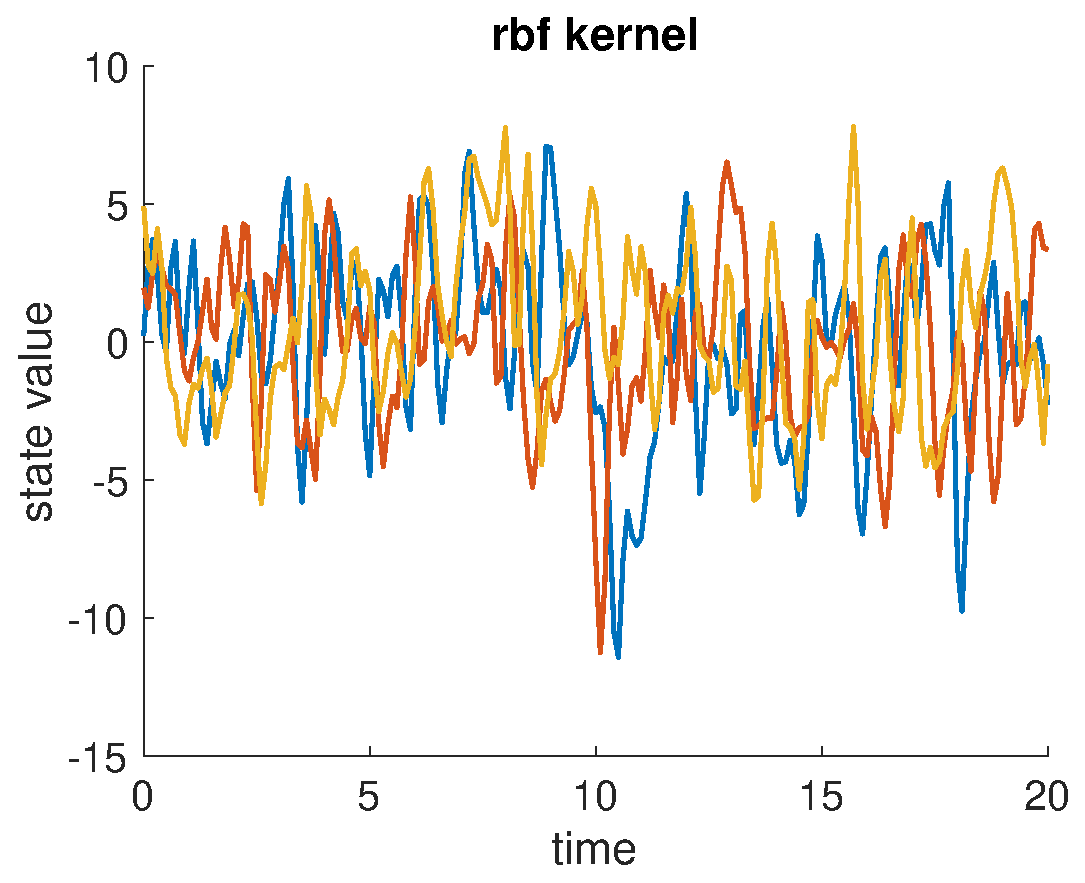
\includegraphics [width=4in]{Lorenz_attractor_4_04.eps}
\begin{par}
determine $\mathbf{A} + \mathbf{I}\gamma$:
\end{par} \vspace{1em}
\begin{verbatim}
A = ddC - dC_times_invC * Cd;
A_plus_gamma = A + state.derivative_variance(1) .* eye(size(A));
A_plus_gamma = 0.5.*(A_plus_gamma+A_plus_gamma');  % ensure that A plus gamma is symmetric
A_plus_gamma_inv = inv_chol(chol(A_plus_gamma,'lower'));
\end{verbatim}
\begin{verbatim}
end
\end{verbatim}
\begin{par}
\ensuremath{\backslash}subsection\{ Fitting state observations \}
\end{par} \vspace{1em}
\begin{par}
We fit the observations of state trajectories by standard GP regression.
\end{par} \vspace{1em}
\begin{par}
$p(\mathbf{X} \mid \mathbf{Y}, \phi,\gamma) = \prod_k \mathcal{N}(\mathbf{x}_k ; \boldmath\mu_k(\mathbf{y}_k),\boldmath\Sigma_k)$,
\end{par} \vspace{1em}
\begin{par}
where $\boldmath\mu_k(\mathbf{y}_k) := \sigma_k^{-2} \left(\sigma_k^{-2} \mathbf{I} + \mathbf{C}_{\boldmath\phi_k}^{-1} \right)^{-1} \mathbf{y}_k$ and $\boldmath\Sigma_k ^{-1}:=\sigma_k^{-2} \mathbf{I} + \mathbf{C}_{\boldmath\phi_k}^{-1}$.
\end{par} \vspace{1em}
\begin{verbatim}
function [mu_u,inv_sigma_u,state] = fitting_state_observations(state,inv_C,...
    obs_to_state_relation,simulation)
\end{verbatim}
\begin{par}
Dimensions
\end{par} \vspace{1em}
\begin{verbatim}
numb_states = size(state.sym.mean,2);
numb_time_points = size(state.sym.mean,1);
\end{verbatim}
\begin{par}
Variance of state observations
\end{par} \vspace{1em}
\begin{verbatim}
state_obs_variance = simulation.state_obs_variance(state.obs);
\end{verbatim}
\begin{par}
Form block-diagonal matrix out of $\mathbf{C}_{\boldmath\phi_k}^{-1}$
\end{par} \vspace{1em}
\begin{verbatim}
inv_C_replicas = num2cell(inv_C(:,:,ones(1,numb_states)),[1,2]);
inv_C_blkdiag = sparse(blkdiag(inv_C_replicas{:}));
\end{verbatim}
\begin{par}
GP posterior inverse covariance matrix: $\boldmath\Sigma_k ^{-1}:=\sigma_k^{-2} \mathbf{I} + \mathbf{C}_{\boldmath\phi_k}^{-1}$
\end{par} \vspace{1em}
\begin{verbatim}
dim = size(state_obs_variance,1)*size(state_obs_variance,2);
% covariance matrix of error term (big E):
D = spdiags(reshape(state_obs_variance.^(-1),[],1),0,dim,dim) * speye(dim);
A_times_D_times_A = obs_to_state_relation' * D * obs_to_state_relation;
inv_sigma = A_times_D_times_A + inv_C_blkdiag;
\end{verbatim}
\begin{par}
GP posterior mean: $\boldmath\mu_k(\mathbf{y}_k) := \sigma_k^{-2} \left(\sigma_k^{-2} \mathbf{I} + \mathbf{C}_{\boldmath\phi_k}^{-1} \right)^{-1} \mathbf{y}_k$
\end{par} \vspace{1em}
\begin{verbatim}
mu = inv_sigma \ obs_to_state_relation' * D * reshape(state.obs,[],1);
\end{verbatim}
\begin{par}
Reshape GP mean
\end{par} \vspace{1em}
\begin{verbatim}
mu_u = zeros(numb_time_points,numb_states);
for u = 1:numb_states
    idx = (u-1)*numb_time_points+1:(u-1)*numb_time_points+numb_time_points;
    mu_u(:,u) = mu(idx);
end
\end{verbatim}
\begin{par}
Reshape GP inverse covariance matrix
\end{par} \vspace{1em}
\begin{verbatim}
inv_sigma_u = zeros(numb_time_points,numb_time_points,numb_states);
for i = 1:numb_states
    idx = [(i-1)*numb_time_points+1:(i-1)*numb_time_points+numb_time_points];
    inv_sigma_u(:,:,i) = inv_sigma(idx,idx);
end
\end{verbatim}
\begin{verbatim}
end
\end{verbatim}
\begin{par}
\ensuremath{\backslash}subsection\{ Find state ODE couplings \}
\end{par} \vspace{1em}
\begin{verbatim}
function coupling_idx = find_state_couplings_in_odes(ode,symbols)

state_sym = sym('state%d',[1,length(ode.system)]); assume(state_sym,'real');
for k = 1:length(ode.system)
    tmp_idx = ismember(state_sym,symvar(ode.system_sym(k))); tmp_idx(:,k) = 1;
    ode_couplings_states(k,tmp_idx) = 1;
end

for u = 1:length(symbols.state)
    coupling_idx.states{u} = find(ode_couplings_states(:,u));
end
end
\end{verbatim}
\begin{par}
\ensuremath{\backslash}subsection\{ Rewrite ODEs as linear combination in parameters \}
\end{par} \vspace{1em}
\begin{par}
$\mathbf{B}_{\theta k} \theta + \mathbf{b}_{\theta k} \stackrel{!}{=} \mathbf{f}_k(\mathbf{X},\theta)$,
\end{par} \vspace{1em}
\begin{par}
where matrices $\mathbf{B}_{\theta k}$ and $\mathbf{b}_{\theta k}$ are defined such that the ODEs $\mathbf{f}_k(\mathbf{X},\theta)$ are expressed as a linear combination in $\theta$.
\end{par} \vspace{1em}
\begin{verbatim}
function [B,b] = rewrite_odes_as_linear_combination_in_parameters(ode,symbols)
\end{verbatim}
\begin{par}
Initialization of symbolic variables
\end{par} \vspace{1em}
\begin{verbatim}
param_sym = sym('param%d',[1,length(symbols.param)]); assume(param_sym,'real');
state_sym = sym('state%d',[1,length(symbols.state)]); assume(state_sym,'real');
state0_sym = sym('state0'); assume(state0_sym,'real');
state_const_sym = sym('state_const'); assume(state_const_sym,'real');
\end{verbatim}
\begin{par}
Rewrite ODEs as linear combinations in parameters (global)
\end{par} \vspace{1em}
\begin{verbatim}
[B_sym,b_sym] = equationsToMatrix(ode.system_sym,param_sym);
b_sym = -b_sym; % See the documentation of the function "equationsToMatrix"
\end{verbatim}
\begin{par}
Operations locally w.r.t. ODEs
\end{par} \vspace{1em}
\begin{verbatim}
for k = 1:length(ode.system)
    B_sym(k,B_sym(k,:)=='0') = state0_sym;
    for i = 1:length(B_sym(k,:))
        sym_var = symvar(B_sym(k,i));
        if isempty(sym_var)
            B_sym(k,i) = B_sym(k,i) + state0_sym;
        end
    end
    B{k} = matlabFunction(B_sym(k,:),'Vars',{state_sym,state0_sym,state_const_sym});
    b{k} = matlabFunction(b_sym(k,:),'Vars',{state_sym,state0_sym,state_const_sym});
end
\end{verbatim}
\begin{verbatim}
end
\end{verbatim}
\begin{par}
\ensuremath{\backslash}subsection\{ Rewrite ODEs as linear combination in individual states \}
\end{par} \vspace{1em}
\begin{par}
$\mathbf{R}_{uk} \mathbf{x}_u + \mathbf{r}_{uk} \stackrel{!}{=} \mathbf{f}_k(\mathbf{X},\theta)$.
\end{par} \vspace{1em}
\begin{par}
where matrices $\mathbf{R}_{uk}$ and $\mathbf{r}_{uk}$ are defined such that the ODEs $\mathbf{f}_k(\mathbf{X},\theta)$ is rewritten as a linear combination in the individual state $\mathbf{x}_u$.
\end{par} \vspace{1em}
\begin{verbatim}
function [R,r] = rewrite_odes_as_linear_combination_in_ind_states(ode,symbols,coupling_idx)
\end{verbatim}
\begin{par}
Initialization of symbolic variables
\end{par} \vspace{1em}
\begin{verbatim}
param_sym = sym('param%d',[1,length(symbols.param)]); assume(param_sym,'real');
state_sym = sym('state%d',[1,length(symbols.state)]); assume(state_sym,'real');
state0_sym = sym('state0'); assume(state0_sym,'real');
state_const_sym = sym('state_const'); assume(state_const_sym,'real');
\end{verbatim}
\begin{par}
Rewrite ODEs as linear combinations in parameters (locally)
\end{par} \vspace{1em}
\begin{verbatim}
for u = 1:length(symbols.state)
    for k = coupling_idx{u}'
        [R_sym,r_sym] = equationsToMatrix(ode.system{k}(state_sym,param_sym'),...
            state_sym(:,u));
        r_sym = -r_sym; % See the documentation of the function "equationsToMatrix"

        R{u,k} = matlabFunction(R_sym,'Vars',{state_sym,param_sym});
        r{u,k} = matlabFunction(r_sym,'Vars',{state_sym,param_sym});
    end
end
\end{verbatim}
\begin{verbatim}
end
\end{verbatim}
\begin{par}
\ensuremath{\backslash}subsection\{ Proxy for ODE parameters \}
\end{par} \vspace{1em}
\begin{par}
$\hat{q}(\theta) {\propto} \exp \bigg( ~E_{Q_{-\theta}}  \ln \mathcal{N}\left(\theta ; \left( \mathbf{B}_{\theta}^T \mathbf{B}_{\theta} \right)^{-1} \left( \sum_k \mathbf{B}_{\theta k}^T ~ \left( {'\mathbf{C}_{\phi k}} \mathbf{C}_{\phi k}^{-1} \mathbf{X}_k - \mathbf{b}_{\theta k} \right) \right), ~ \mathbf{B}_{\theta}^+ ~ (\mathbf{A} + \mathbf{I}\gamma) ~ \mathbf{B}_{\theta}^{+T} \right) ~\bigg)$,
\end{par} \vspace{1em}
\begin{verbatim}
function [param_proxy_mean,param_proxy_inv_cov] = ...
    proxy_for_ode_parameters(state_proxy_mean,dC_times_invC,lin_comb,symbols,...
    A_plus_gamma_inv,opt_settings)
\end{verbatim}
\begin{par}
Initialization
\end{par} \vspace{1em}
\begin{verbatim}
state0 = zeros(size(dC_times_invC,1),1);
param_proxy_inv_cov = zeros(length(symbols.param));
global_scaling = zeros(length(symbols.param));
global_mean = zeros(length(symbols.param),1);
\end{verbatim}
\begin{par}
Iteratate through ODEs
\end{par} \vspace{1em}
\begin{verbatim}
for k = 1:length(symbols.state)
\end{verbatim}
\begin{par}
unpack matrices $\mathbf{B}$ and $\mathbf{b}$
\end{par} \vspace{1em}
\begin{verbatim}
    B = lin_comb.B{k}(state_proxy_mean,state0,ones(size(state_proxy_mean,1),1));
    b = lin_comb.b{k}(state_proxy_mean,state0,ones(size(state_proxy_mean,1),1));
\end{verbatim}
\begin{par}
Local operations
\end{par} \vspace{1em}
\begin{verbatim}
    if strcmp(opt_settings.pseudo_inv_type,'Moore-Penrose')
\end{verbatim}
\begin{par}
The Moore-Penrose inverse of $\mathbf{B}_{\theta}$ is given by: $\mathbf{B}_{\theta}$ is given by: $\mathbf{B}_{\theta}^+ := \left(\mathbf{B}_{\theta}^T \mathbf{B}_{\theta} \right)^{-1} \mathbf{B}_{\theta}^T$
\end{par} \vspace{1em}
\begin{par}
local mean: $\mathbf{B}_{\theta k}^T ~ \left( {'\mathbf{C}_{\phi_k}} \mathbf{C}_{\phi k}^{-1} \mathbf{X}_k - \mathbf{b}_{\theta k} \right)$
\end{par} \vspace{1em}
\begin{verbatim}
        local_mean = B' * (dC_times_invC * state_proxy_mean(:,k) - b);
        local_scaling = B' * B;
        local_inv_cov = B' * A_plus_gamma_inv * B;
\end{verbatim}
\begin{verbatim}
    elseif strcmp(opt_settings.pseudo_inv_type,'modified Moore-Penrose')
\end{verbatim}
\begin{par}
The modified Moore-Penrose inverse of $\mathbf{B}_{\theta}$ is given by: $\mathbf{B}_{\theta}$ is given by: $\mathbf{B}_{\theta}^+ := \left(\mathbf{B}_{\theta}^T (\mathbf{A} + \mathbf{I}\gamma) \mathbf{B}_{\theta} \right)^{-1} \mathbf{B}_{\theta}^T (\mathbf{A} + \mathbf{I}\gamma)$
\end{par} \vspace{1em}
\begin{par}
local mean: $\mathbf{B}_{\theta k}^T (\mathbf{A} + \mathbf{I}\gamma) ~ \left( {'\mathbf{C}_{\phi_k}} \mathbf{C}_{\phi k}^{-1} \mathbf{X}_k - \mathbf{b}_{\theta k} \right)$
\end{par} \vspace{1em}
\begin{verbatim}
        local_mean = B' * A_plus_gamma_inv * (dC_times_invC * state_proxy_mean(:,k) - b);
        local_scaling = B' * A_plus_gamma_inv * B;
        local_inv_cov = local_scaling;
\end{verbatim}
\begin{verbatim}
    end
\end{verbatim}
\begin{par}
Global operations
\end{par} \vspace{1em}
\begin{verbatim}
    global_mean = global_mean + local_mean;
    global_scaling = global_scaling + local_scaling;

    % Inverse covariance of ODE param proxy distribution
    param_proxy_inv_cov = param_proxy_inv_cov + local_inv_cov;
\end{verbatim}
\begin{verbatim}
end
\end{verbatim}
\begin{par}
Check scaling of covariance matrix
\end{par} \vspace{1em}
\begin{verbatim}
[~,D] = eig(param_proxy_inv_cov);
if any(diag(D)<0)
    warning('param_proxy_inv_cov has negative eigenvalues!');
elseif any(diag(D)<1e-3)
    warning('param_proxy_inv_cov is badly scaled')
    disp('perturbing diagonal of param_proxy_inv_cov')
    perturb = abs(max(diag(D))-min(diag(D))) / 10000;
    param_proxy_inv_cov(logical(eye(size(param_proxy_inv_cov,1)))) = ...
        param_proxy_inv_cov(logical(eye(size(param_proxy_inv_cov,1)))) ...
        + perturb.*rand(size(param_proxy_inv_cov,1),1);
end
\end{verbatim}
\begin{par}
Mean of parameter proxy distribution (option: Moore-penrose inverse example):
\end{par} \vspace{1em}
\begin{par}
$\left( \mathbf{B}_{\theta}^T \mathbf{B}_{\theta} \right)^{-1} \left( \sum_k \mathbf{B}_{\theta k}^T ~ \left( {'\mathbf{C}_{\phi k}} \mathbf{C}_{\phi k}^{-1} \mathbf{X}_k - \mathbf{b}_{\theta k} \right) \right)$
\end{par} \vspace{1em}
\begin{verbatim}
param_proxy_mean = global_scaling \ global_mean;
param_proxy_mean = abs(param_proxy_mean);      % mirroring to preserve magnitude
\end{verbatim}
\begin{verbatim}
end
\end{verbatim}
\begin{par}
\ensuremath{\backslash}subsection\{ Proxy for individual states \}
\end{par} \vspace{1em}
\begin{par}
$\hat{q}(\mathbf{x}_u) \propto \exp\big( ~ E_{Q_{-u}} \ln \mathcal{N}\left(\mathbf{x}_u ; \left( \mathbf{B}_{u} \mathbf{B}_{u}^T \right)^{-1} \left( - \sum_k \mathbf{B}_{uk}^T \mathbf{b}_{uk} \right), ~\mathbf{B}_{u}^{+} ~ (\mathbf{A} + \mathbf{I}\gamma) ~ \mathbf{B}_u^{+T} \right)$
\end{par} \vspace{1em}
\begin{par}
$\qquad \qquad \qquad \qquad \qquad + E_{Q_{-u}} \ln \mathcal{N}\left(\mathbf{x}_u ; \boldmath\mu_u(\mathbf{Y}), \Sigma_u \right) \big)$,
\end{par} \vspace{1em}
\begin{verbatim}
function [state_proxy_mean,state_proxy_inv_cov] = proxy_for_ind_states(lin_comb,...
    state_proxy_mean,ode_param,dC_times_invC,coupling_idx,symbols,mu,inv_sigma,...
    observed_states,A_plus_gamma_inv,opt_settings)
\end{verbatim}
\begin{par}
Indices of observed states
\end{par} \vspace{1em}
\begin{verbatim}
tmp = cellfun(@(x) {strcmp(x,observed_states)},symbols.state);
state_obs_idx = cellfun(@(x) any(x),tmp);
\end{verbatim}
\begin{par}
Clamp observed states to GP fit
\end{par} \vspace{1em}
\begin{verbatim}
if opt_settings.clamp_obs_state_to_GP_fit
    state_enumeration = find(~state_obs_idx);
else
    state_enumeration = 1:length(symbols.state);
end
\end{verbatim}
\begin{par}
Iterate through states
\end{par} \vspace{1em}
\begin{verbatim}
for u = state_enumeration
\end{verbatim}
\begin{par}
Initialization
\end{par} \vspace{1em}
\begin{verbatim}
    state_proxy_inv_cov(:,:,u) = zeros(size(dC_times_invC));
    global_scaling = zeros(size(dC_times_invC));
    global_mean = zeros(size(dC_times_invC,1),1);
\end{verbatim}
\begin{par}
Iteratate through ODEs
\end{par} \vspace{1em}
\begin{verbatim}
    for k = coupling_idx{u}'
\end{verbatim}
\begin{par}
unpack matrices $\mathbf{R}$ and $\mathbf{r}$
\end{par} \vspace{1em}
\begin{verbatim}
        R = diag(lin_comb.R{u,k}(state_proxy_mean,ode_param));
        r = lin_comb.r{u,k}(state_proxy_mean,ode_param);
        if size(R,1) == 1; R = R.*eye(size(dC_times_invC,1)); end
        if length(r)==1; r = zeros(length(global_mean),1); end
\end{verbatim}
\begin{par}
Define matrices B and b such that $\mathbf{B}_{uk} \mathbf{x}_u + \mathbf{b}_{uk} \stackrel{!}{=} \mathbf{f}_k(\mathbf{X},\theta) - {'\mathbf{C}}_{\phi_{k}} \mathbf{C}_{\phi_{k}}^{-1} \mathbf{X}$
\end{par} \vspace{1em}
\begin{verbatim}
        if k~=u
            B = R;
            b = r - dC_times_invC * state_proxy_mean(:,k);
        else
            B = R - dC_times_invC;
            b = r;
        end
\end{verbatim}
\begin{par}
Local operations
\end{par} \vspace{1em}
\begin{verbatim}
        if strcmp(opt_settings.pseudo_inv_type,'Moore-Penrose')
            % local mean: $\mathbf{B}_{uk}^T \left(\epsilon_0^{(k)}
            % -\mathbf{b}_{uk}
            local_mean = -B' * b;
            local_scaling = B' * B;
            local_inv_cov = B' * A_plus_gamma_inv * B;
        elseif strcmp(opt_settings.pseudo_inv_type,'modified Moore-Penrose')
            local_mean = -B' * A_plus_gamma_inv * b;
            local_scaling = B' * A_plus_gamma_inv * B;
            local_inv_cov = local_scaling;
        end
\end{verbatim}
\begin{par}
Global operations
\end{par} \vspace{1em}
\begin{verbatim}
        global_mean = global_mean + local_mean;
        global_scaling = global_scaling + local_scaling;
\end{verbatim}
\begin{par}
Inverse covariance for state proxy distribution
\end{par} \vspace{1em}
\begin{verbatim}
        state_proxy_inv_cov(:,:,u) = state_proxy_inv_cov(:,:,u) + local_inv_cov;
\end{verbatim}
\begin{verbatim}
    end
\end{verbatim}
\begin{par}
Mean of state proxy distribution (option: Moore-penrose inverse example): $\left( \mathbf{B}_{u} \mathbf{B}_{u}^T \right)^{-1} \sum_k \mathbf{B}_{uk}^T \left(\epsilon_0^{(k)} -\mathbf{b}_{uk} \right)$
\end{par} \vspace{1em}
\begin{verbatim}
    state_proxy_mean(:,u) = (global_scaling + inv_sigma(:,:,u)) \ (global_mean + ...
        (inv_sigma(:,:,u) * mu(:,u)));
\end{verbatim}
\begin{verbatim}
end
\end{verbatim}
\begin{verbatim}
end
\end{verbatim}
\begin{par}

\end{par} \vspace{1em}
\begin{verbatim}
function generate_Lorenz96_ODEs(numb_odes)

for i = 1:numb_odes
    state{i} = ['[x_' num2str(i) ']'];
end
param = '[\theta]';

ode{1} = ['(' state{2} ' - ' state{end-1} ') .* ' state{end} ' - ' state{1} ' + ' param];
ode{2} = ['(' state{3} ' - ' state{end} ') .* ' state{1} ' - ' state{2} ' + ' param];
for i = 3:numb_odes-1
    ode{i} = [ '(' state{i+1} ' - ' state{i-2} ') .* ' state{i-1} ' - ' state{i} ' + ' param];
end
ode{numb_odes} = ['(' state{1} ' - ' state{end-2} ') .* ' state{end-1} ' - ' state{end} ' + ' param];

dlmwrite('Lorenz96_ODEs.txt',[])

for i = 1:numb_odes
    dlmwrite('Lorenz96_ODEs.txt',char(ode{i}),'delimiter','','-append')
end
end
\end{verbatim}
\begin{par}
\ensuremath{\backslash}subsection\{ Import ODEs \}
\end{par} \vspace{1em}
\begin{verbatim}
function ode = import_odes(symbols,odes_path)
\end{verbatim}
\begin{par}
Import ODEs expressions
\end{par} \vspace{1em}
\begin{verbatim}
ode.raw = importdata(odes_path);
ode.refined = ode.raw;
\end{verbatim}
\begin{par}
Refine ODEs
\end{par} \vspace{1em}
\begin{verbatim}
for k = 1:length(ode.refined)
for u = 1:length(symbols.state)
    ode.refined{k} = strrep(ode.refined{k},[symbols.state{u}],['state(:,' num2str(u) ')']);
end
for j = 1:length(symbols.param)
    ode.refined{k} = strrep(ode.refined{k},symbols.param{j},['param(' num2str(j) ')']);
end
end
for k = 1:length(ode.refined)
    ode.system{k} = str2func(['@(state,param)(' ode.refined{k} ')']);
end
\end{verbatim}
\begin{verbatim}
end
\end{verbatim}
\begin{par}
\ensuremath{\backslash}subsection\{ Generate ground truth \}
\end{par} \vspace{1em}
\begin{verbatim}
function [state,time,ode] = generate_ground_truth(time,state,ode,symbols,simulation,...
    odes_path)
\end{verbatim}
\begin{par}
Integration times
\end{par} \vspace{1em}
\begin{verbatim}
time.true=0:simulation.int_interval:simulation.final_time;   % true times
TTT=length(simulation.time_samp);    % number of sampled points
% Index of sample time in the true time
itrue=round(simulation.time_samp./simulation.int_interval+ones(1,TTT));
\end{verbatim}
\begin{par}
Symbolic computations
\end{par} \vspace{1em}
\begin{verbatim}
param_sym = sym('param%d',[1,length(symbols.param)]); assume(param_sym,'real');
state_sym = sym('state%d',[1,length(symbols.state)]); assume(state_sym,'real');
for i = 1:length(ode.system)
    ode.system_sym(i) = ode.system{i}(state_sym,param_sym);
end
\end{verbatim}
\begin{par}
Fourth order Runge-Kutta (numerical) integration
\end{par} \vspace{1em}
\begin{verbatim}
if ~strcmp(odes_path,'Lorenz96_ODEs.txt')
    ode_system_mat = matlabFunction(ode.system_sym','Vars',{state_sym',param_sym'});
    [~,OutX_solver]=ode45(@(t,x) ode_system_mat(x,simulation.ode_param'), time.true, ...
        simulation.init_val);
else
    OutX_solver = create_Lorenz96(min(time.true),max(time.true),time.true(2)-time.true(1),...
        state.derivative_variance',[simulation.ode_param, length(state_sym)])';ToutX = time.true';
end
state.true_all=OutX_solver;
state.true=state.true_all(itrue,:);
\end{verbatim}
\begin{verbatim}
end
\end{verbatim}
\begin{par}
\ensuremath{\backslash}subsection\{ Generate observations of states \}
\end{par} \vspace{1em}
\begin{verbatim}
function [state,time,obs_to_state_relation] = generate_state_obs(state,time,simulation,...
    symbols)
\end{verbatim}
\begin{verbatim}
tmp = cellfun(@(x) {strcmp(x,simulation.observed_states)},symbols.state);
state_obs_idx = cellfun(@(x) any(x),tmp);
\end{verbatim}
\begin{par}
State observations
\end{par} \vspace{1em}
\begin{verbatim}
state_obs_variance = simulation.state_obs_variance(state.true(:,state_obs_idx));
state.obs = state.true(:,state_obs_idx) + sqrt(state_obs_variance) .* ...
    randn(size(state.true(:,state_obs_idx)));
\end{verbatim}
\begin{par}
Mapping between states and observations
\end{par} \vspace{1em}
\begin{verbatim}
if length(simulation.time_samp) < length(time.est)
    time.idx = munkres(pdist2(simulation.time_samp',time.est'));
    time.ind = sub2ind([length(simulation.time_samp),length(time.est)],...
        1:length(simulation.time_samp),time.idx);
else
    time.idx = munkres(pdist2(time.est',simulation.time_samp'));
    time.ind = sub2ind([length(time.est),length(simulation.time_samp)],...
        1:length(time.est),time.idx);
end
time.obs_time_to_state_time_relation = zeros(length(simulation.time_samp),...
    length(time.est));
time.obs_time_to_state_time_relation(time.ind) = 1;
state_mat = eye(size(state.true,2));
state_mat(~state_obs_idx,:) = [];
obs_to_state_relation = sparse(kron(state_mat,time.obs_time_to_state_time_relation));
time.samp = simulation.time_samp;
\end{verbatim}
\begin{verbatim}
end
\end{verbatim}
\begin{par}
\ensuremath{\backslash}subsection\{ Setup plots \}
\end{par} \vspace{1em}
\begin{verbatim}
function [h_states,h_param,p] = setup_plots(state,time,simulation,symbols,plot_settings)
\end{verbatim}
\begin{par}
Indices of observed states
\end{par} \vspace{1em}
\begin{verbatim}
tmp = cellfun(@(x) {strcmp(x,simulation.observed_states)},symbols.state);
state_obs_idx = cellfun(@(x) any(x),tmp);
obs_ind = find(state_obs_idx);
\end{verbatim}
\begin{par}
Refine ODE parameter symbols
\end{par} \vspace{1em}
\begin{verbatim}
for i = 1:length(symbols.param); symbols.param{i} = symbols.param{i}(2:end-1); end
\end{verbatim}
\begin{par}
Figure size and position setup
\end{par} \vspace{1em}
\begin{verbatim}
figure(1); set(1,'Position',[0,200,plot_settings.size(1),plot_settings.size(2)]);
\end{verbatim}

\includegraphics [width=4in]{Lorenz_attractor_4_01.eps}
\begin{par}
ODE parameters
\end{par} \vspace{1em}
\begin{verbatim}
h_param = subplot(plot_settings.layout(1),plot_settings.layout(2),1);
h_param.FontSize = 20; h_param.Title.String = 'ODE parameters';
h_param.Title.FontWeight = 'Normal';
set(gca,'XTick',[1:length(symbols.param)]); set(gca,'XTickLabel',symbols.param);
hold on; drawnow

nStates_plot=length(symbols.state);if nStates_plot > 8; nStates_plot = 8; end
\end{verbatim}

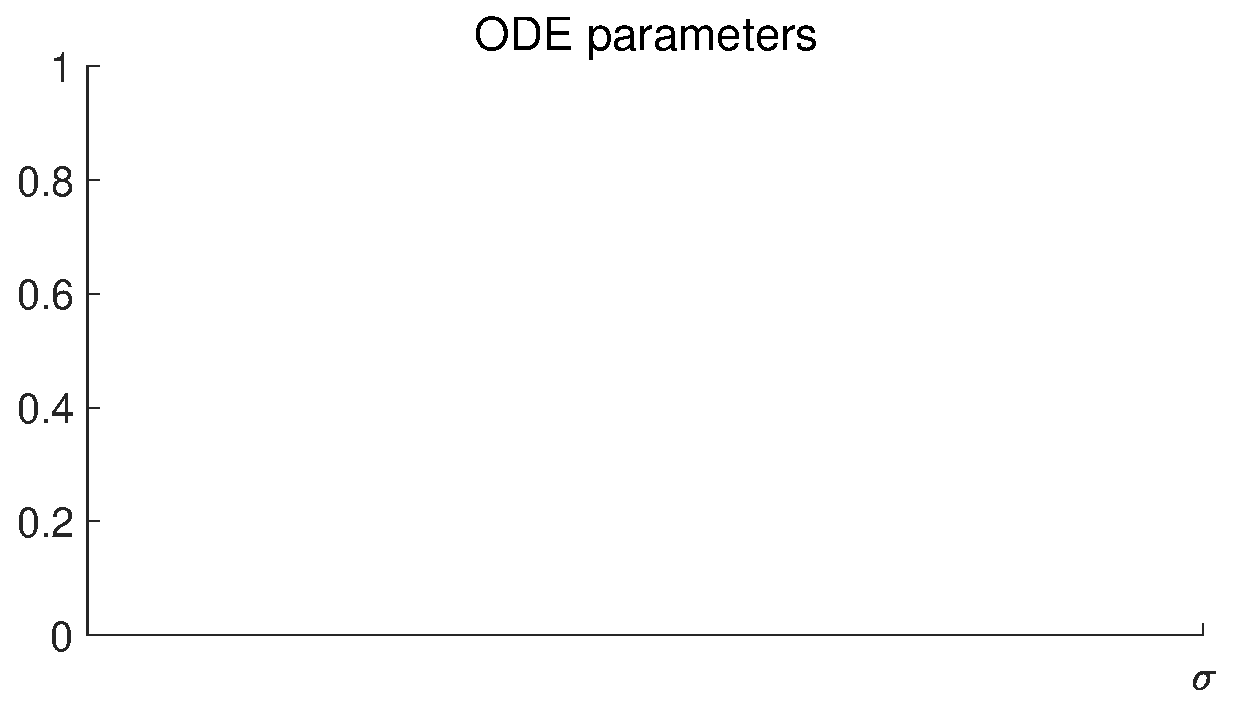
\includegraphics [width=4in]{Lorenz_attractor_4_02.eps}
\begin{par}
States
\end{par} \vspace{1em}
\begin{verbatim}
u2=0;
for u = 1:nStates_plot
    h_states{u} = subplot(plot_settings.layout(1),plot_settings.layout(2),u+1); cla;
    p.true = plot(time.true,state.true_all(:,u),'LineWidth',2,'Color',[217,95,2]./255);
    h_states{u}.Title.String = symbols.state{u}(2:end-1);
    hold on;
    if any(obs_ind==u)
        u2=u2+1;
        p.obs = plot(simulation.time_samp,state.obs(:,u2),'*','Color',...
            [217,95,2]./255,'MarkerSize',10);
    end
    h_states{u}.FontSize = 20;
    if any(obs_ind==u)
        h_states{u}.Title.String = symbols.state{u}(2:end-1);
    else
        h_states{u}.Title.String = ['unobserved ' symbols.state{u}(2:end-1)];
    end
    h_states{u}.Title.FontWeight = 'Normal';
    h_states{u}.XLim = [min(time.est),max(time.est)];
    h_states{u}.XLabel.String = 'time'; hold on;
end
\end{verbatim}

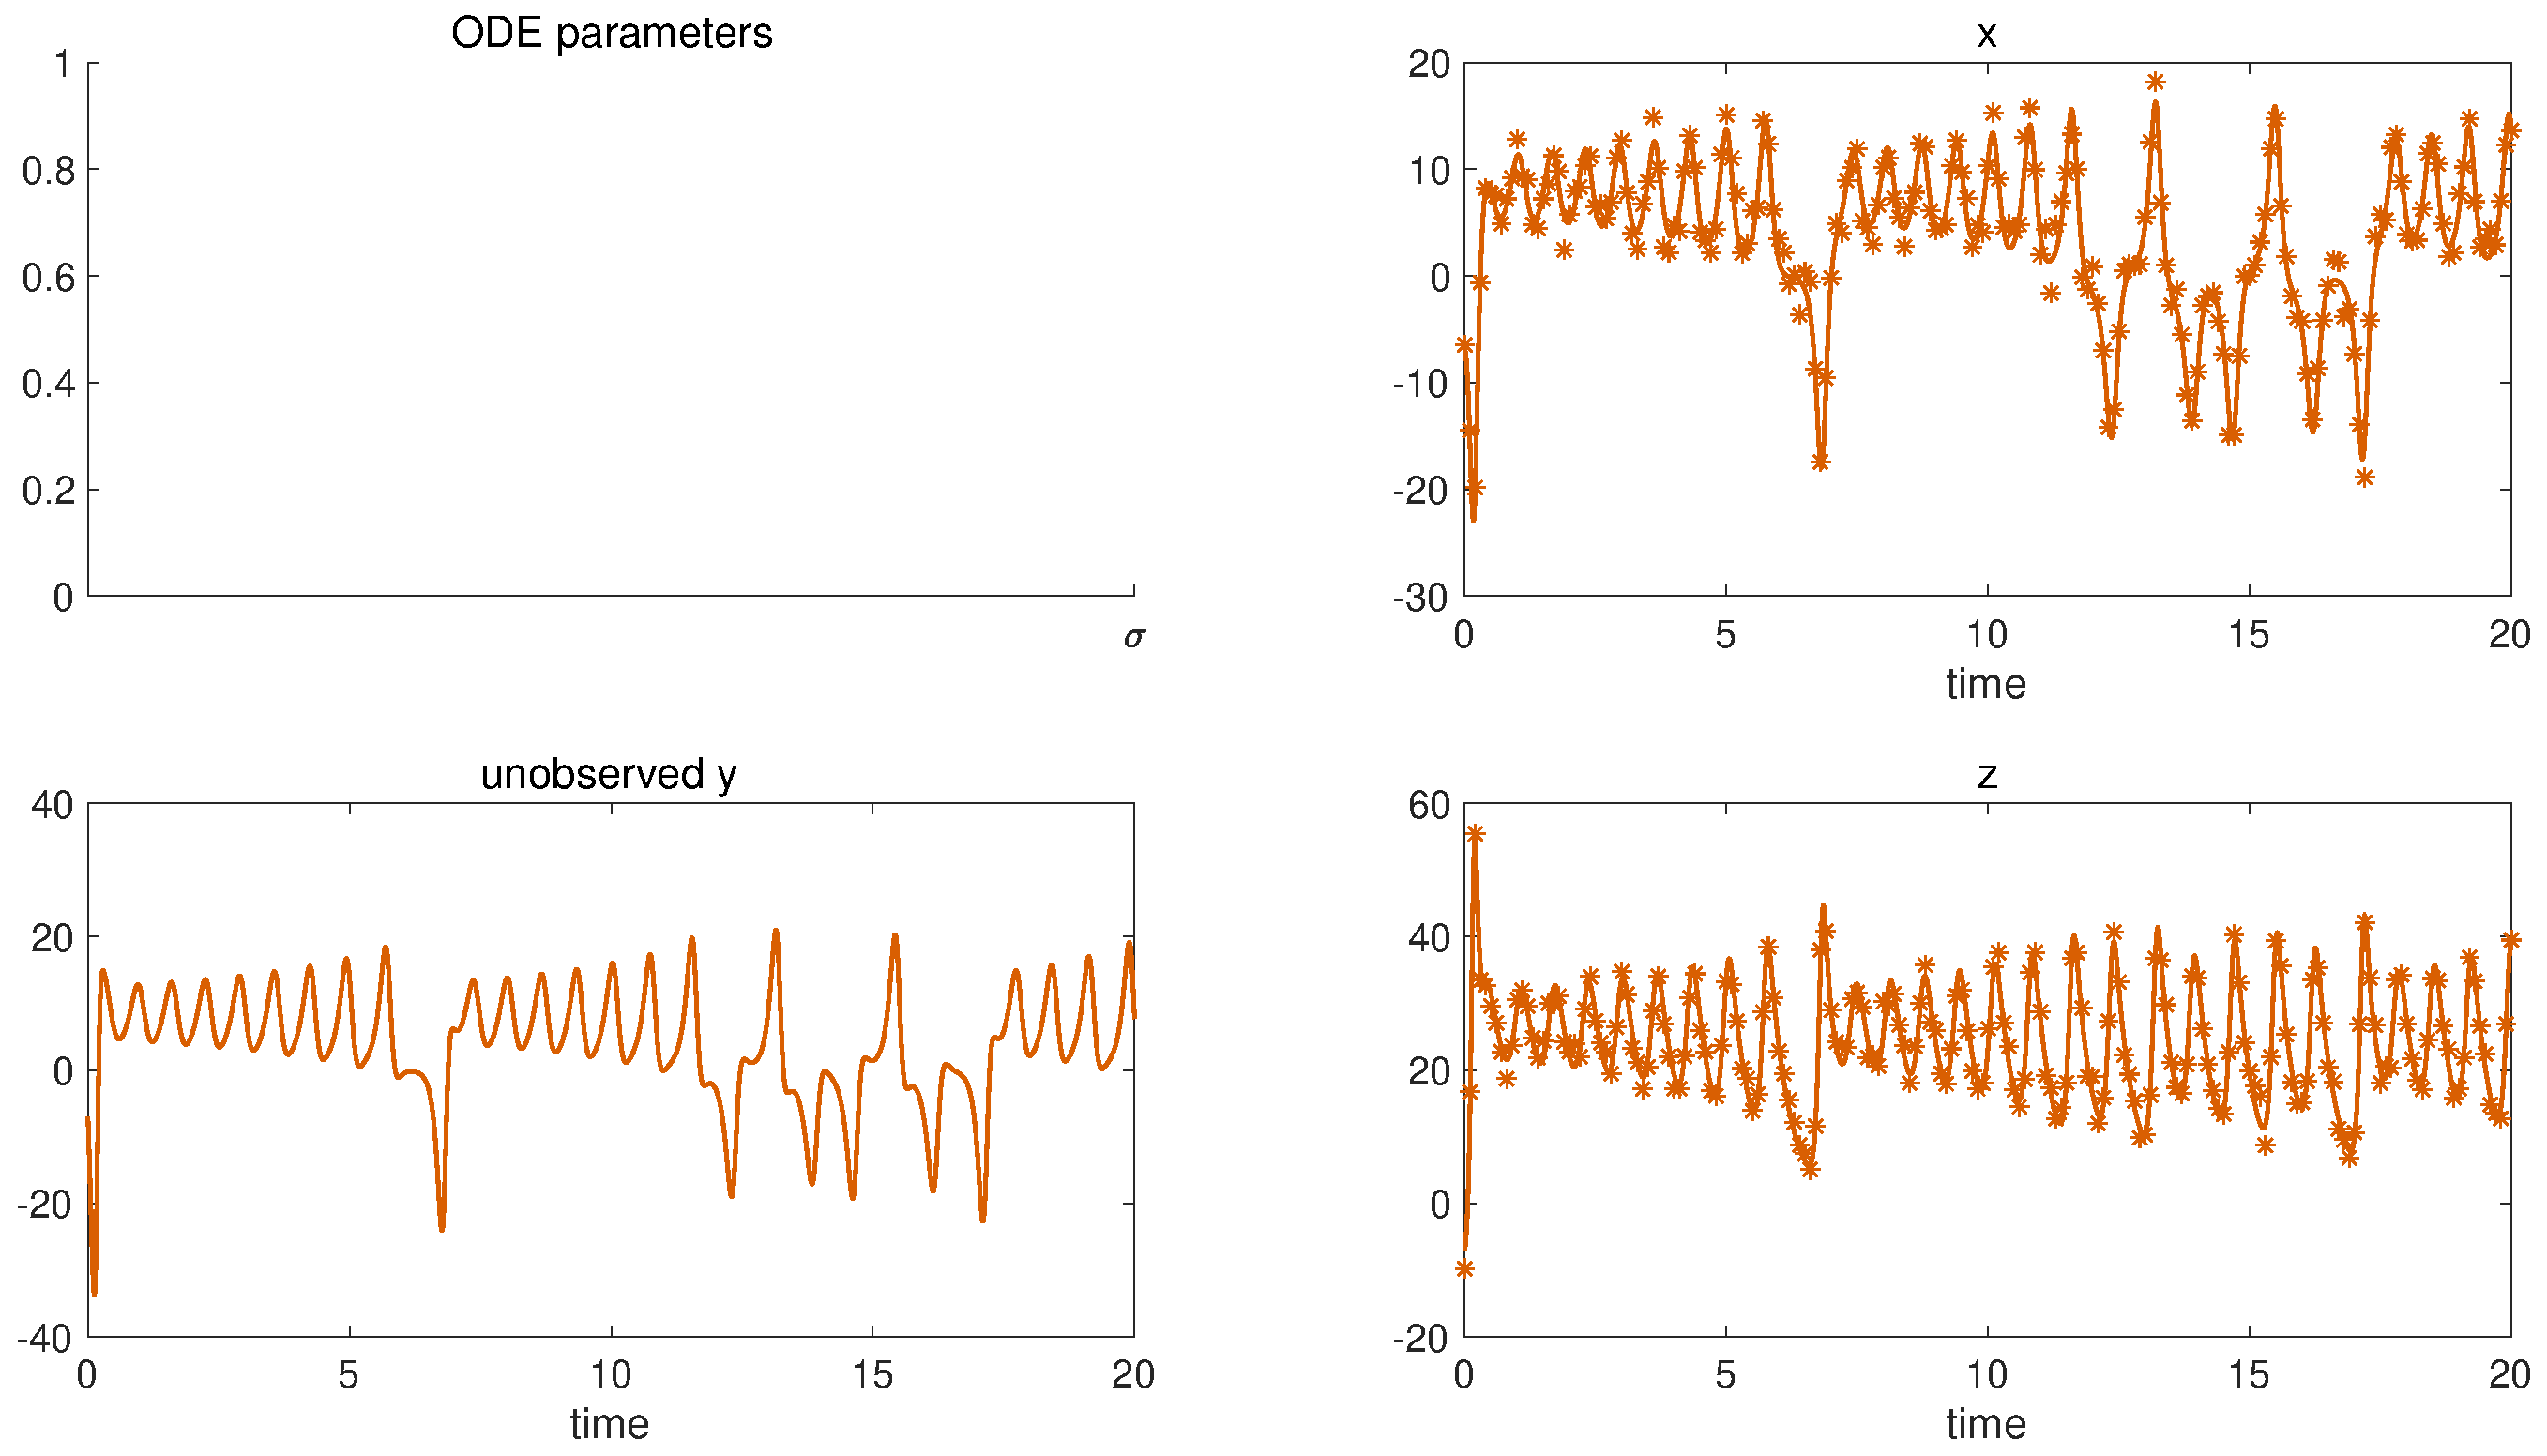
\includegraphics [width=4in]{Lorenz_attractor_4_03.eps}
\begin{verbatim}
end
\end{verbatim}
\begin{par}
\ensuremath{\backslash}subsection\{ Plot results \}
\end{par} \vspace{1em}
\begin{verbatim}
function plot_results(h_states,h_param,state,time,simulation,param_proxy_mean,p,...
    symbols,plot_type)

% Indices of observed states
tmp = cellfun(@(x) {strcmp(x,simulation.observed_states)},symbols.state);
state_obs_idx = cellfun(@(x) any(x),tmp);
obs_ind = find(state_obs_idx);

nStates_plot=length(symbols.state);if nStates_plot > 8; nStates_plot = 8; end

u2=0;
for u = 1:nStates_plot
    if strcmp(plot_type,'final')

        % State proxy variance
        if ~any(obs_ind==u)
            state_proxy_variance = diag(state.proxy.inv_cov(:,:,u)^(-1));
            shaded_region = [state.proxy.mean(:,u)+1*sqrt(state_proxy_variance);
                flip(state.proxy.mean(:,u)-1*sqrt(state_proxy_variance),1)];
            f = fill(h_states{u},[time.est'; flip(time.est',1)], shaded_region,...
                [222,235,247]/255);
            set(f,'EdgeColor','None');
        end

        % Replot true states
        p.true = plot(h_states{u},time.true,state.true_all(:,u),'LineWidth',...
            2,'Color',[217,95,2]./255);

        % Replot state observations
        if any(obs_ind==u)
            u2=u2+1;
            p.obs = plot(h_states{u},simulation.time_samp,state.obs(:,u2),...
                '*','Color',[217,95,2]./255,'MarkerSize',10);
        end

        % State proxy mean (final)
        hold on;
        p.est = plot(h_states{u},time.est,state.proxy.mean(:,u),'Color',...
            [117,112,179]./255,'LineWidth',2);
    else
        % state proxy mean (not final)
        hold on; p.est = plot(h_states{u},time.est,state.proxy.mean(:,u),...
            'LineWidth',0.1,'Color',[0.8,0.8,0.8]);
    end
    % Specify legend entries
    if state_obs_idx(u)
        legend(h_states{u},[p.true,p.obs,p.est],{'true','observed','estimate'},...
            'Location','southwest','FontSize',12);
    else
        legend(h_states{u},[p.true,p.est],{'true','estimate'},'Location',...
            'southwest','FontSize',12);
    end
end

% ODE parameters
cla(h_param);
try
    b = bar(h_param,1:length(param_proxy_mean),[simulation.ode_param',...
        param_proxy_mean]);
catch
    b = bar(h_param,1:length(param_proxy_mean)+1,[[simulation.ode_param';0],...
        [param_proxy_mean;0]]);
end
b(1).FaceColor = [217,95,2]./255; b(2).FaceColor = [117,112,179]./255;
h_param.XLim = [0.5,length(param_proxy_mean)+0.5]; h_param.YLimMode = 'auto';
legend(h_param,{'true','estimate'},'Location','northwest','FontSize',12);
drawnow
end
\end{verbatim}



\end{document}
    
